\documentclass{book}

\usepackage{graphicx}
\usepackage{moreverb}
\usepackage{amsmath}
\usepackage{alltt}
\usepackage{rotating}
\usepackage{subfigure}
\usepackage{toc}
\usepackage{xspace}
\usepackage{makeidx}

\newcommand{\extref}[1]{$\S$\ref*{#1}}   % No hyperlink. For external refs. \extref
\newcommand{\comma}{\> ,}
\newcommand{\period}{\> .}
\newcommand{\wt}{\widetilde}
\newcommand{\grv}{\textasciigrave}
\newcommand{\hyperbf}[1]{\textbf{\hyperpage{#1}}}
\newcommand{\Ss}{\(^*\)}
\newcommand{\Dd}{\(^\dagger\)}

\newcommand{\AND}{&& \hskip -17pt\relax}
\newcommand{\CR}{\\}
\newcommand{\CRNO}{\nonumber \\}
\newcommand{\dstyle}{\displaystyle}

\newcommand{\Begineq}{\begin{equation}}
\newcommand{\Endeq}{\end{equation}}
\newcommand{\NoPrint}[1]{}

\newcommand{\pow}[1]{\cdot 10^{#1}}
\newcommand{\Bf}[1]{{\bf #1}}
\newcommand{\bfr}{\Bf r}

\newcommand{\bmad}{{\sl Bmad}\xspace}
\newcommand{\tao}{{\sl Tao}\xspace}
\newcommand{\mad}{{\sl MAD}\xspace}
\newcommand{\cesr}{{\sl CESR}\xspace}

\newcommand{\sref}[1]{\S\ref{#1}}
\newcommand{\Sref}[1]{Sec.~\sref{#1}}
\newcommand{\cref}[1]{Chapter~\ref{#1}}

\newcommand{\Newline}{\hfil \\ \relax}

\newcommand{\eq}[1]{{(\protect\ref{#1})}}
\newcommand{\Eq}[1]{{Eq.~(\protect\ref{#1})}}
\newcommand{\Eqs}[1]{{Eqs.~(\protect\ref{#1})}}

\newcommand{\vn}{\ttcmd}           % For variable names
\newcommand{\vni}{\ttcmdindx}
\newcommand{\cs}{\ttcmd}           % For code source
\newcommand{\cmd}{\ttcmd}          % For Unix commands
\newcommand{\rn}{\ttcmd}           % For Routine names
\newcommand{\tn}{\ttcmd}           % For Type (structure) names
\newcommand{\bn}[1]{{\bf #1}}       
\newcommand{\toffset}{\vskip 0.01in}
\newcommand{\rot}[1]{\begin{rotate}{-45}#1\end{rotate}}

\newcommand{\data}{{\mbox{data}}}
\newcommand{\reference}{{\mbox{ref}}}
\newcommand{\model}{{\mbox{model}}}
\newcommand{\base}{{\mbox{base}}}
\newcommand{\design}{{\mbox{design}}}
\newcommand{\meas}{{\mbox{meas}}}
\newcommand{\var}{{\mbox{var}}}

\newcommand\ttcmd{\begingroup\catcode`\_=11 \catcode`\%=11 \dottcmd}
\newcommand\dottcmd[1]{\texttt{#1}\endgroup}

\newcommand\ttcmdindx{\begingroup\catcode`\_=11 \catcode`\%=11 \dottcmdindx}
\newcommand\dottcmdindx[1]{\texttt{#1}\endgroup\index{#1}}

\newcommand{\St}{$^{st}$\xspace}
\newcommand{\Nd}{$^{nd}$\xspace}
\newcommand{\Th}{$^{th}$\xspace}
\newcommand{\B}{$\backslash$}
\newcommand{\W}{$^\wedge$}

\newcommand{\cbar}[1]{\overline C_{#1}}

\newlength{\dPar}
\setlength{\dPar}{1.5ex}

\newenvironment{example}
  {\vspace{-3.0ex} \begin{alltt}}
  {\end{alltt} \vspace{-2.5ex}}

\newcommand\Strut{\rule[-2ex]{0mm}{6ex}}

\newenvironment{Itemize}
  {\begin{list}{$\bullet$}
    {\addtolength{\topsep}{-1.5ex} 
     \addtolength{\itemsep}{-1ex}
    }
  }
  {\end{list} \vspace*{1ex}}

\newcommand{\Section}[1]{\section{#1}\indent\vspace{-3ex}}

\newcommand{\SECTION}[1]{\section*{#1}\indent\vspace{-3ex}}

% From pg 64 of The LaTex Companion.

\newenvironment{ventry}[1]
  {\begin{list}{}
    {\renewcommand{\makelabel}[1]{\textsf{##1}\hfil}
     \settowidth{\labelwidth}{\textsf{#1}}
     \addtolength{\itemsep}{-1.5ex}
     \addtolength{\topsep}{-1.0ex} 
     \setlength{\leftmargin}{5em}
    }
  }
  {\end{list}}


\setlength{\textwidth}{6.25in}
\setlength{\hoffset}{0.0in}
\setlength{\oddsidemargin}{0.25in}
\setlength{\evensidemargin}{0.0in}
\setlength{\textheight}{8.5in}
\setlength{\topmargin}{0in}

\makeindex

\begin{document}

\index{Reference orbit|see{Coordinates, reference orbit}}
\index{Global coordinates|see{Coordinates, global}}
\index{Floor coordinates|see{Coordinates, global}}
\index{Phase space|see{Coordinates, phase space}}
\index{FPP|see{PTC/FPP}}
\index{Forest, Etienne|see{PTC/FPP}}
\index{Bmad!lattice format|see{Lattice file format}}
\index{Radiation damping and excitation|see{Synchrotron radiation}}
\index{Coupling|see{Normal mode}}
\index{Variables|see{Lattice file format, variables}}
\index{Taylor map|see{Transfer map, Taylor}}
\index{Transfer map!mat6_calc_method|see{mat6_calc_method}}
\index{Map|see{Transfer map}}
\index{Beam line|see{Line}}
\index{Replacement List|see{List}}
\index{Functions|see{Intrinsic functions}}
\index{Arithmetic expressions!intrinsic functions|see{Intrinsic functions}}
\index{Ring_struct!%param|see{Param_struct}}
\index{Lattice files!XSIF|see{XSIF}}
\index{An|see{Multipole, an}}
\index{Bn|see{Multipole, bn}}
\index{KnL|see{Multipole, knl}}
\index{Tn|see{Multipole, tn}}

%----------------------------------------------------------------
\thispagestyle{empty}

\begin{flushright}
\large
  Revision: 0.3.2 \\
  April 30, 2006 \\
\end{flushright}

\vfill

{
\begin{center}
{\Huge \sf\bf The} \\
\vskip 0.1in
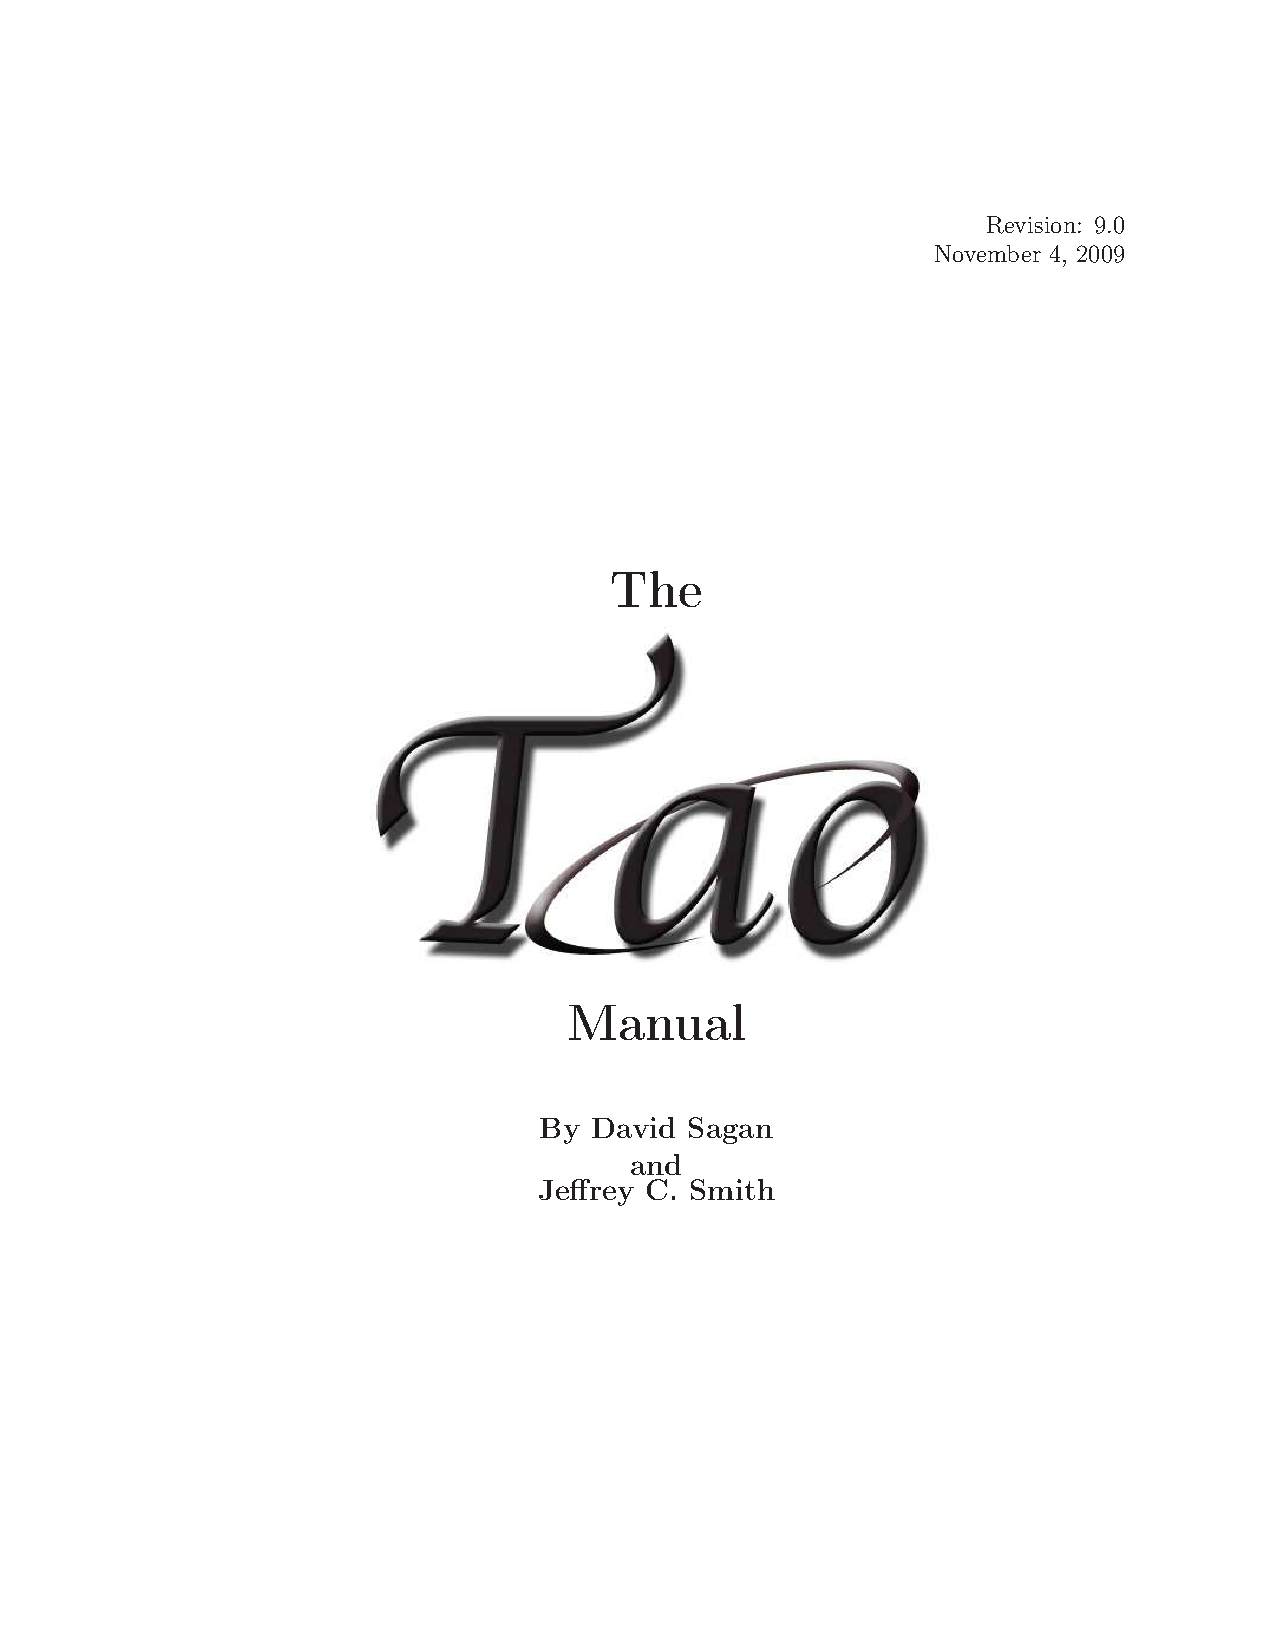
\includegraphics[width=10cm]{tao.psfig} \\
\vskip 0.1in
{\Huge \sf\bf Manual} \\
\vskip 0.4in
{\Large \sf\bf By David Sagan \\ and \\ Jeffrey C. Smith} \\
\end{center}
}

\vskip 1in
\begin{center}
{\Huge \bf *** DRAFT ***}
\end{center}
\vfill
\break


%----------------------------------------------------------------
{
\setlength{\parskip}{\dPar}
\setlength{\parindent}{0ex}
\chapter{Overview: Starting and Running Tao}
\label{c:overview.tao}

%----------------------------------------------------------------
\section{Tao Setup}
\label{s:obtaining}

Instructions for obtaining and for setting up \tao can be found at:
\begin{example}
  www.lepp.cornell.edu/bmad/
\end{example}

%----------------------------------------------------------------
\section{Tao Tutorial}
\label{s:tutorial}

This manual is organized more as a reference guide than as a tutorial so for an introduction
to \tao (and \bmad) there is a link on the web page at:
\begin{example}
  www.lepp.cornell.edu/bmad/tao.html
\end{example}

%-----------------------------------------------------------------
\section{Initialization from the Command Line}
\index{command line}
\label{s:command.line} 

The syntax of the command line for running \tao is:
\begin{example}
  EXE-DIRECTORY/tao \{OPTIONS\}
\end{example}
where \vn{EXE-DIRECTORY} is the directory where the tao executable lives. If this directory is
listed in your \vn{PATH} environmental variable then the directory specification may be omitted.
The optional arguments are:
%
\begin{description}
%
\item[\vn{-beam <beam_file>}] \Newline
Overrides the \vn{beam_file} (\sref{s:init.global}) specified in the
\tao initialization file.
%
  \item[\vn{-beam_all <all_beam_file>}] \Newline
Overrides the \vn{beam_all_file} (\sref{s:beam.init}) specified in the
\vn{tao_beam_init} namelist.
%
\item[\vn{-beam_init_file_name <file_name>}] \Newline
Overrides the \vn{beam_init%file_name} (\sref{s:beam.init}) specified in the
\vn{tao_beam_init} namelist.
%
\item[\vn{-building_wall <wall_file>}] \Newline
Overrides the \vn{building_wall_file} (\sref{s:init.global}) 
specified in the \tao initialization file.
%
\item[\vn{-data <data_file>}] \Newline
Overrides the \vn{data_file} (\sref{s:init.global}) specified in the
\tao initialization file.
%
\item[\vn{-disable_smooth_line_calc}] \Newline
Disable computation of the ``smooth curves'' used in plotting. 
This can be used to speed up \tao as discussed in \sref{s:plot.data}.
%
\item[\vn{-geometry <width>x<height>}] \Newline
Overrides the plot window geometry. \vn{<width>} and \vn{<height>}
are in Points. This is equivalent to setting \vn{plot_page%size}
in the \vn{tao_plot_page} namelist \sref{s:init.plot}.
%
\item[\vn{-hook_init_file}] \Newline
Specifies an input file for customized versions of Tao. Default file
name is \vn{tao_hook.init}.
%
\item[\vn{-init <tao_init_file>}] \Newline
replaces the default \tao initialization file name
(\vn{tao.init}). Note: A \tao initialization file is actually not
needed. If no \tao initialization file is used, the use of the
\vn{-lat} switch is mandatory and \tao will use a set of default plot
templates for plotting.
%
\item[\vn{-lat <bmad_or_xsif_lattice_file>}] \Newline
Overrides the \vn{design_lattice}
lattice file specified in the \tao initialization file
(\sref{s:init.lat}). Example:
\begin{example}
  tao -init my.init -lat slac.xsif
\end{example}
If there is more than one universe and the universes have different
lattices, separate the different lattice names using a "|" character.
Do not put any spaces in between. Example:
\begin{example}
  tao -lat xsif::slac.lat|cesr.bmad
\end{example}
%
\item[\vn{-log_startup}]
If there is a problem with \tao is started, \vn{-log_startup} can be used
to create a log file of the initialization process.
%
\item[\vn{-no_stopping}] \Newline
For debugging purposes. Prevents \tao from stopping where there is a fatal error.
%
\item[\vn{-noinit}] \Newline
Suppresses use of a \tao initialization file. In this case the use of
the \vn{-lat} switch is mandatory and \tao will use a set of default
plot templates for plotting.
%
\item[\vn{-noplot}] \Newline
Suppresses the opening of the plot window.
%
\item[\vn{-plot <plot_file>}] \Newline
Overrides the \vn{plot_file} (\sref{s:init.global}) specified in the
\tao initialization file.
%
\item[\vn{-prompt_color}] \Newline
Sets the prompt string color to Blue. For different colors, use the
\vn{set global prompt_color} command (\sref{s:set}).
%
\item[\vn{-rf_on}]
Leaves \vn{rfcavity} elements on. Normally \tao turns off these elements
since Twiss and dispersion calculations do not make sense with them on.
%
\item[\vn{-slice_lattice <element_list>}]
If present, discard from the lattice all lattice elements that are not in the \vn{<element_list>}.
Overrides the setting of \vn{design_lattice(i)%slice_lattice}.
%
\item[\vn{-startup <startup_command_file>}]
Overrides the \vn{startup_file} (\sref{s:init.global}) specified in the
\tao initialization file.
%
\item[\vn{-var <var_file>}] \Newline
Overrides the \vn{var_file} (\sref{s:init.global}) specified in the
\tao initialization file.

\end{description}

%----------------------------------------------------------------
\section{Initializing Tao}
\index{initializing!files}
\label{s:initializing}

Initialization occurs when \tao is started. Initialization information is stored in one or more
files as discussed in Chapter \sref{c:init}. If no initialization files are found. \tao uses a
default initialization.

%----------------------------------------------------------------
\section{Command Line Mode and Single Mode}
\label{s:modes}

After \tao is initialized, \tao interacts with the user though the command line. \tao has two modes
for this. In \vn{command line} mode, which is the default mode, \tao waits until the the \vn{return}
key is depressed to execute a command. Command line mode is described in Chapter~\sref{c:command}. 

In \vn{single} mode, single keystrokes are interpreted as commands. \tao can be set up so that in
\vn{single mode} the pressing of certain keys increase or decrease variables. While the same effect
can be achieved in the standard \vn{line mode}, \vn{single mode} allows for quick adjustments of
variables. See Chapter~\sref{c:single} for more details.

%-----------------------------------------------------------------
\section{Lattice Calculations}
\index{lattice calculaitons}
\label{s:lat.calc.overview} 

By default \tao recalculates lattice parameters and does tracking of particles after each command.
The exception is for commands that do not change any parameter that would affect such calculations
such as the \vn{show} command. See \sref{s:lat.calc} for more details. If the recalculation takes a
significant amount of time, the recalculation may be suppressed using the \vn{set global
lattice_calc_on} command (\sref{s:set.global}) or the \vn{set universe} command
(\sref{s:set.universe}).

%-----------------------------------------------------------------
\section{Command Files and Aliases}
\index{command files}
\label{s:command.files} 

Typing repetitive commands in command line mode can become tedious. \tao has two constructs to
mitigate this: Aliases and Command Files. 

Aliases are just like aliases in Unix. See Section~\sref{s:alias} for more details.

Command files are like Unix shell scripts. A series of commands are
put in a file and then that file can be called using the \vn{call}
command (\sref{s:call}).

\tao will call a command file at startup. The default name of this startup file is \vn{tao.startup}
but this name can be changed (\sref{s:format}).

Do loops (\sref{s:do}) are allowed with the following syntax:
\begin{example}
  do <var> = <begin>, <end> \{, <step>\} 
    ...
    tao command [[<var>]]
    ...
  enddo
\end{example}
The \vn{<var>} can be used as a variable in the loop body but must be
bracketed ``[[<var>]]''.  The step size can be any integer positive or
negative but not zero.  Nested loops are allowed and command files can
be called within do loops.

\begin{example}
  do i = 1, 100
    call set_quad_misalignment [[i]] ! command file to misalign quadrupoles
    zero_quad 1e-5*2^([[i]]-1) ! Some user supplied command to zero quad number [[i]]
  enddo
\end{example}

To reduce unnecessary calculations, the logicals \vn{global%lattice_calc_on}
and \vn{global%plot_on} can be toggled from within the command file. Example
\begin{example}
  set global lattice_calc_on = F  ! Turn off lattice calculations
  set global plot_on = F          ! Turn off plot calculations
  ... do some stuff ...
  set global plot_on = T          ! Turn back on 
  set global lattice_calc_on = T  ! Turn back on
\end{example}
Additionally, the \vn{global%command_file_print_on} switch controls
whether printing is suppressed when a command file is called.

A \vn{end_file} command (\sref{s:end.file}) can be used to signal the
end of the command file.

The \vn{pause} command (\sref{s:pause}) can be used to temporarily
pause the command file.

%----------------------------------------------------------------
\section{Customizing Tao}
\label{s:cust.tao}

Custom code can be linked with \tao to extend \tao's capabilities. For example, \tao can be extended to
be used as an online model in a control system. See Chapter~\sref{c:custom.tao} for more details.

\section*{Introduction}

The strength of \bmad is that, as a subroutine library, it provides a
flexible framework from which sophisticated simulation programs may
easily be developed.  The weakness of \bmad comes from its strength:
\bmad cannot be used straight out of the box. Someone must put the
pieces together into a program. This means that \bmad is
complementary to a general purpose program like
\MAD\cite{b:maduser,b:madphysics}: If \mad can solve the problem at
hand you don't need \bmad. If there are no programs that do what you
want, or they are too slow, then \bmad is very useful.

As a consequence of \bmad being a software library this manual serves
two masters: The programmer who wants to develop applications and
needs to know about the inner workings of \bmad, and the user who
simply needs to know about the \bmad standard input format and about
the physics behind the various calculations that \bmad performs.

To this end, this manual is divided into three parts. The first two
parts are for both the user and programmer while the third part is
meant just for programmers. Part~I gives the conventions used by
\bmad --- coordinate systems, magnetic field expansions, etc. ---
along with some of the physics behind the calculations. By necessity,
the physics documentation is brief and the reader is assumed to be familiar
with high energy accelerator physics formalism. Part~II discusses the
\bmad lattice input standard.  The \bmad lattice input standard was
developed using the \mad lattice input standard as a starting
point. \mad (Methodical Accelerator Design) is a widely used
stand--alone program developed at CERN by Christoph Iselin for
charged--particle optics calculations. Since it can be convenient
to do simulations with both \mad and \bmad, differences and
similarities between the two input formats are noted. 
Finally, Part~III gives the nitty--gritty details of the \bmad
subroutines and the structures upon which they are based.

More information, including the most up--to--date version of this
manual, can be found at the \bmad web site at
\begin{example}
  http://www.lepp.cornell.edu/~dcs/bmad
\end{example}
\index{Bmad!information}

Errors and omissions are a fact of life for any reference work and
comments from you, dear reader, are therefore most welcome. Please
send any missives (or chocolates, or any other kind of sustenance) to:
\begin{example}
  David Sagan <dcs16@cornell.edu>
\end{example}
\index{Bmad!error reporting}

It is my pleasure to express appreciation to people who have
contributed to this effort: To David Rubin for his support, to Etienne
Forest for use of his remarkable PTC/FPP library not to mention his
patience in explaining everything to me, to Mark Palmer for all his
work porting \bmad to different platforms, to Hans Grote for granting
the adaptation of figures in the \mad manual for use in this one, to
Richard Helms, Kim Moore, Jeremy Urban, Jeff Smith, and Mike Forster
for their help, and last but not least to my wife Flora who put up
with me at 1am in the morning when I was working on \bmad.


}

%----------------------------------------------------------------
\tableofcontents
\listoffigures
\listoftables

%----------------------------------------------------------------
\setlength{\parskip}{\dPar}
\setlength{\parindent}{0ex}
\part{Conventions and Physics}

%----------------------------------------------------------------
\chapter{Coordinates}
\index{coordinates|hyperbf}

%-----------------------------------------------------------------------------
\section{Local Reference Orbit}
\label{s:ref}
\index{reference orbit|hyperbf}

\begin{figure}[!b]
  \centering
  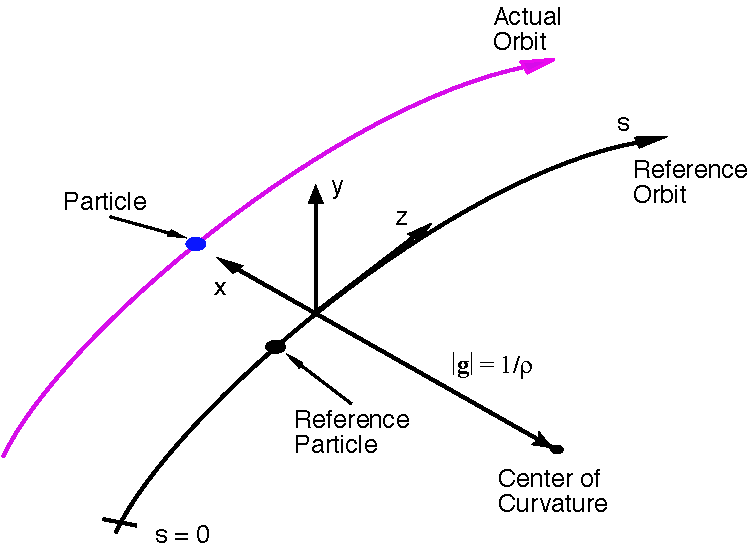
\includegraphics[height=8.4cm]{local-coords.pdf}
  \caption[The local Reference System.]
{The local reference coordinate system. By construction, a particle's
$z$ coordinate is zero.  This is not to be confused with the phase
space $z$ coordinate (\sref{s:phase.space}). The curvature vector
$\bfg$ lies in the $x$-$y$ plane and has a magnitude of $1/\rho$ where
$\rho$ is the bending radius. The $z$-axis will normally be parallel
to the $s$-axis but for reversed elements it will be antiparallel.
}
  \label{f:local.coords}
\end{figure}

The \vn{local reference orbit} is the curved path used to define a
coordinate system for describing a particle's position as shown in
\fig{f:local.coords}. The reference orbit is also used for orientating
lattice elements in space. At a given time $t$, a particle's position
can be described by a point on the reference orbit a distance $s$
relative to the reference orbit's zero position plus a transverse
offset. This point on the reference orbit is used as the origin of the
local $(x, y, z)$ coordinate system with the $z$--axis tangent to the
reference orbit. The $z$--axis will generally be pointing in the
direction of increasing $s$ but, as discussed in detail below, will
point counter to $s$ for elements that are reversed. The $x$ and
$y$--axes are perpendicular to the reference orbit. As will be shown
later, If the lattice has no vertical bends, the $y$--axis is in the
vertical direction and the $x$--axis is in the horizontal
plane. Notice that, by construction, the particle is always at $z =
0$. The coordinate system so constructed is called the \vn{``local
coordinate system''} or sometimes the \vn{``laboratory coordinate
system''} when there is need to distinguish it from the \vn{``element
coordinate system''} (\sref{s:ele.coords}) which is attached to
the physical element.

There is a separate reference orbit for each branch
(\sref{s:branch.def}) of a lattice. When there are multiple branches,
the reference orbit of a branch must not depend upon the configuration
of branches later on in the array of branches in the lattice. As a
consequence, the reference orbits of the branches can be calculated
one at a time starting with the first branch.

\index{x_offset}\index{y_offset}
\index{x_pitch}\index{y_pitch}\index{wiggler}
Notice that, in a \vn{wiggler}, the reference orbit, which is a
straight line, does {\em not} correspond to the orbit that any actual
particle could travel. Typically the physical element is
centered with respect to the reference curve. However, by specifying offsets, 
pitches or a tilt (See \sref{s:offset}), the physical element may be
arbitrarily shifted with respect to its reference curve. Shifting a
physical magnet with respect to its reference curve generally means
that the reference curve does {\em not} correspond to the orbit that
any actual particle could travel.

Do not confuse this reference orbit (which defines the local
coordinate system) with the reference orbit about which the transfer
maps are calculated (\sref{s:twiss}). The former is fixed by the
lattice while the latter can be any arbitrary orbit.

%-----------------------------------------------------------------------------
\section{Reference Orbit Construction}
\label{s:ref.construct}
\index{reference orbit!construction}

%--------------------------------------

  \begin{figure}[tb]
  \centering
  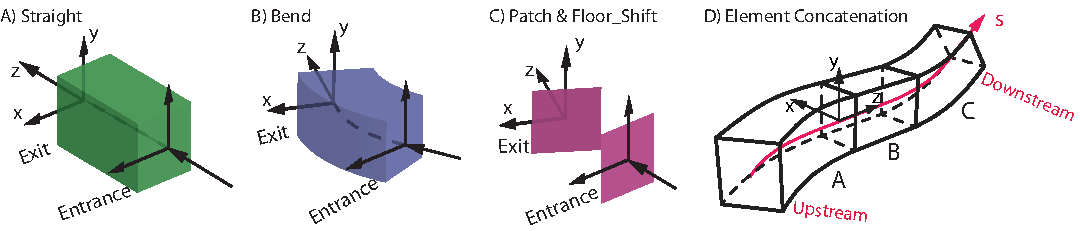
\includegraphics{element-coord-frame.pdf}
\caption[Element LEGO blocks.]{Element reference frame LEGO
blocks. Shown are the blocks along with the entrance and exit
reference frames. The physical element may be displaced in the local
coordinate frame using offsets, tilt, and pitches. A) For straight
line elements the two frames are colinear. B) For bends elements, the
two frames are rotated with respect to each other. C) For \vn{patch}
and \vn{floor_shift} elements the exit frame may be arbitrarily
positioned with respect to the entrance.}
  \label{f:ele.coord.frame}
  \end{figure}

%--------------------------------------

\begin{figure}[tb]
  \centering
  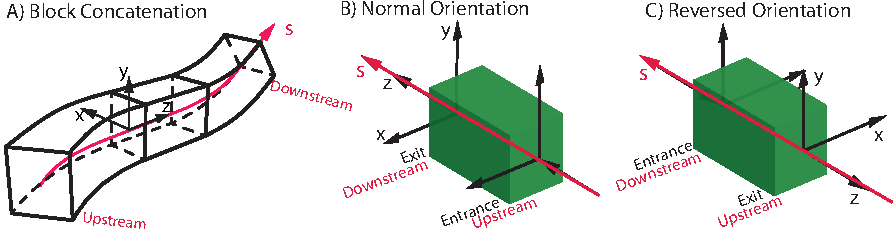
\includegraphics{element-stream.pdf}
  \caption[Element LEGO block concatenation.]{
Element LEGO block concatenation. A) The reference orbit is
constructed by concatenating the LEGO blocks together. B) For normal
(non-reversed) elements the $z$-axis is parallel with the $s$-axis. C)
For reversed elements the $z$-axis is antiparallel with the
$s$-axis. By definition, the ``entrance'' and ``exit'' ends of an
element are fixed relative to the element (relative to the $z$-axis)
while the ``upstream'' and ``downstream'' ends are fixed relative to
the $s$-axis.}
  \label{f:stream}
\end{figure}

%--------------------------------------

\index{sbend}\index{rbend}
\index{crystal}\index{mirror}\index{entrance_end}
\index{exit_end}\index{patch}\index{floor_shift}
Another way of thinking about the reference orbit is to imagine that
each element has assigned to it a local coordinate reference frame
assigned to it in the shape of a LEGO block\footnote{Thanks to Dan
Abell for this analogy.} as shown in \fig{f:ele.coord.frame}.  Every
block has an ``\vn{entrance}'' and an ``\vn{exit}'' reference frame.
For most types of elements, the LEGO block for the element is
``straight'' as shown in \fig{f:ele.coord.frame}A. That is, the
reference curve through the block is a straight line segment and the
length of the block is the length of the element. For a \vn{bend}
(\sref{s:bend}), the reference curve through the block is a segment of
a circular arc as shown in \fig{f:ele.coord.frame}B. With a zero
\vn{ref_tilt}, the rotation axis between the entrance and exit frames of a
bend is the $y$-axis (\sref{s:global}). For \vn{patch}
(\sref{s:patch}), and \vn{floor_shift} (\sref{s:floor.ele}) elements,
the exit face can can arbitrarily oriented with respect to the
entrance end. In this case, the reference orbit between the entrance
and exit faces is not defined.

\index{root branch}
Assuming for the moment that there are no \vn{fiducial} elements
present, the construction of the reference orbit starts at the
beginning element of a branch. If the branch is a \vn{root} branch
(\sref{s:lattice.def}), The orientation of the beginning element can
be set via the appropriate positioning statements
(\sref{s:beginning}). If the branch is not a \vn{root} branch, the
position of the beginning element is determined by the position of the
\vn{fork} or \vn{photon_fork} element from which the branch forks
from.

Once the beginning element in a branch is positioned, succeeding
element LEGO blocks are concatenated together as illustrated in
\fig{f:stream}A. When a block is joined, the end of the block that is
mated to the previous block is called the ``\vn{upstream}'' end and
the other end which will be mated to the following block is called the
``\vn{downstream}'' end.  Normally, the \vn{entrance} end of a block
is used as the \vn{upstream} end the \vn{exit} end is used as the
\vn{downstream} end as shown in \fig{f:stream}B. However, for
\vn{reversed} elements (\sref{s:ele.reverse}), the \vn{upstream} end
is the \vn{exit} end of the block and vice versa. To put it another
way, the \vn{entrance} and \vn{exit} end of the blocks reference the
physical element. Thus, for example, the \vn{e1} edge of a bend
(\sref{s:bend}) is always at the \vn{entrance} face and the \vn{e2} is
always at the \vn{exit}face. Also the field of a wiggler is
(\sref{s:wiggler}) is referenced to $z = 0$ which is at the
\vn{entrance} end. The \vn{upstream} and \vn{downstream} ends, on the
other hand, are referenced to the reference orbit and the
\vn{downstream} end always is at a larger $s$ position relative to the
\vn{upstream} end.

In all cases, when a LEGO block is joined to the previous block, the
coordinate system at the mating end of the block (the \vn{upstream}
end) will be aligned with the mating end of the previous block (the
\vn{downstream} end). The situation where one of the blocks is
reversed and the other one not, and neither is a \vn{patch} nor
\vn{floor_shift} element, does not make physical sense since a
particle which is moving downstream, when it comes to the face joining
the blocks will have to magically reverse direction in order to travel
through the next block. Thus, to have normal and reversed elements in
a branch, \vn{reflection} \vn{patches} must be used in between.
Whether it makes physical sense to put a \vn{patch} element next to
another element is more complicated. This depends upon whether the
other element is reversed or not and whether the \vn{patch} is
reversed, whether the \vn{patch} is \vn{reflecting}, and the sign of
\vn{z_offset} for the \vn{patch}. The basic criterion is that a
particle leaving one block must enter the next. See
Section~\sref{s:ex.patch} for an example.

If there are \vn{fiducial} elements, the local reference frame is
constructed beginning at these elements.

%-----------------------------------------------------------------------------
\section{Global Coordinates}
\label{s:global}
\index{global coordinates|hyperbf}

The Cartesian \vn{global} coordinate system, also called the `floor''
coordinate system, is the coordinate system ``attached to the earth''
that is used to describe the local coordinate system. Following the
\mad\ convention, the \vn{global} coordinate axis are labeled $(X, Y,
Z)$. Conventionally, $Y$ is the ``vertical'' coordinate and $(X, Z)$
are the ``horizontal'' coordinates. To describe how the local
coordinate system is oriented within the global coordinate system,
each point on the $s$-axis of the local coordinate system is
characterized by its $(X, Y, Z)$ position and by three angles $\theta$,
$\phi$, and $\psi$ that describe the orientation of the local coordinate axes
as shown in \fig{f:global.coords}. These three angles are defined as
follows:
\begin{description}
\item[$\theta$ Azimuth angle:] Angle in the $(X, Z)$ plane 
between the $Z$--axis and the projection of the $z$--axis onto the
$(X, Z)$ plane. A positive angle of $\theta = \pi/2$ corresponds to the
projected $z$--axis pointing in the positive $X$ direction.
\item[$\phi$ Pitch (elevation) angle:] Angle between the $z$--axis 
and the $(X,Z)$ plane. A positive angle of $\phi = \pi/2$ corresponds to
the $z$--axis pointing in the positive $Y$ direction.
\item[$\psi$ Roll angle:] Angle of the $x$--axis with respect 
to the line formed by the
intersection of the $(X, Z)$ plane with the $(x, y)$ plane. A
positive $\psi$ forms a right--handed screw with the $z$--axis.
\end{description}

\begin{figure}[tb]
\centering
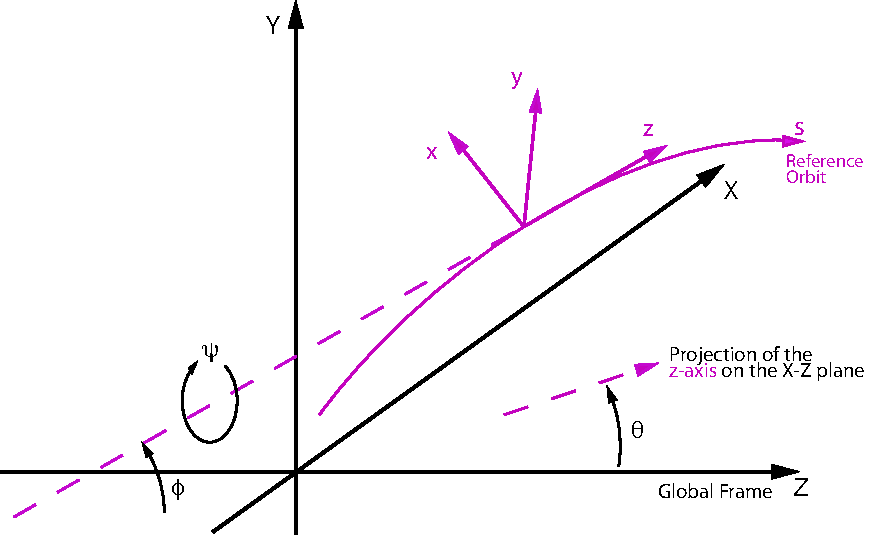
\includegraphics{global-coords.pdf}
\caption[The Global Coordinate System]{The Global Coordinate System.}
\label{f:global.coords}
\end{figure}

\index{beginning statement}
\index{reference orbit!origin in global coordinates}
\index{global coordinates!reference orbit origin}
By default, at $s = 0$, the reference orbit's origin coincides with
the $(X, Y, Z)$ origin and the $x$, $y$, and $z$ axes correspond to
the $X$, $Y$, and $Z$ axes respectively. $\theta$ decreases as one
follows the reference orbit when going through a horizontal bend with
a positive bending angle. This corresponds to $x$ pointing radially
outward. Without any vertical bends, the $Y$ and $y$ axes will
coincide, and $\phi$ and $\psi$ will both be zero. The \vn{beginning}
statement (\sref{s:beginning}) in a lattice file can be use to
override these defaults.

\index{MAD}
Following \mad, the global position of an element is characterized by
a vector $\bfV$ 
\Begineq
  \bfV = 
  \begin{pmatrix}
    X \\ Y \\ Z 
  \end{pmatrix}
\Endeq
The orientation of an element is described by a unitary matrix $\bfW$.
The column vectors of $\bfW$ are the unit vectors spanning the local
coordinate axes in the order $(x, y, z)$. $\bfW$ can be expressed in
terms of the angles $\theta$, $\phi$, and $\psi$ via the formula
\Begineq
  \bfW = \bfW_\Theta \, \bfW_\Phi \, \bfW_\Psi
  \label{wwww}
\Endeq
where
\Begineq
  \bfW_\Theta(\theta) = 
  \begin{pmatrix}
    \cos\theta  & 0 & \sin\theta \\
    0           & 1 & 0          \\
    -\sin\theta & 0 & \cos\theta 
  \end{pmatrix}, \quad
  \bfW_\Phi(\phi) = 
  \begin{pmatrix}
    1 & 0 & 0                \\
    0 & \cos\phi  & \sin\phi \\
    0 & -\sin\phi & \cos\phi 
  \end{pmatrix}, \quad
  \bfW_\Psi(\psi) = 
  \begin{pmatrix}
    \cos\psi & -\sin\psi & 0 \\
    \sin\psi &  \cos\psi & 0 \\
    0        &  0        & 1                
  \end{pmatrix}
  \label{wtt0t}
\Endeq

%-----------------------------------------------------------------------------
\subsection{Lattice Element Positioning}
\label{s:ele.pos}

\index{MAD}
\bmad, again following \mad, computes $\bfV$ and $\bfW$ by starting
at the first element of the lattice and iteratively using the
equations
\begin{align}
  \bfV_i &= \bfW_{i-1} \, \bfL_i + \bfV_{i-1}, 
    \label{vwlv} \\
  \bfW_i &= \bfW_{i-1} \, \bfS_i
    \label{wws}
\end{align}
$\bfL_i$ is the displacement vector for the $i$\Th element and matrix
$\bfS_i$ is the rotation of the local reference system of the exit
end with respect to the entrance end. For clarity, the subscript $i$ in 
the equations below will be dripped. For all elements whose
reference orbit through them is a straight line, the corresponding
$\bfL$ and $\bfS$ are
\Begineq
  \bfL = 
  \begin{pmatrix}
      0 \\ 0 \\ L
  \end{pmatrix},
  \quad
  \bfS = 
  \begin{pmatrix}
      1 & 0 & 0 \\ 
      0 & 1 & 0 \\
      0 & 0 & 1
  \end{pmatrix},
\Endeq
Where $L$ is the length of the element. 

%-----------------------------------------------------------------------

\begin{figure}
\centering 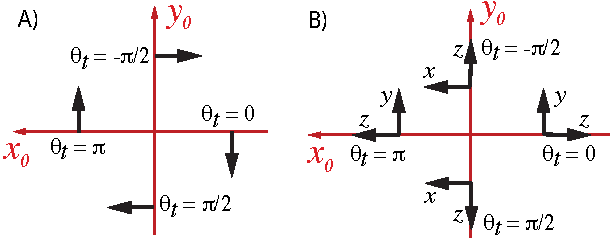
\includegraphics{tilt-bend.pdf} 
\caption[Orientation of a Bend.] 
  {
A) Rotation axes for four different \vn{ref_tilt} angles of $\theta_t$
= 0, $\pm \pi/2$, and $\pi$. $(x_0, y_0, z_0)$ are the local
coordinates at the entrance end of the bend with the $z_0$ axis being
directed into the page. Any rotation axis will be displaced by a
distance of the bend radius \vn{rho} from the origin. B) The $(x, y,
z)$ coordinates at the exit end of the bend for the same four
\vn{ref_tilt} angles. In this case the bend angle is taken to be
$\pi/2$.
  }
  \label{f:tilt.bend}
\end{figure}

%-----------------------------------------------------------------------

\index{rbend}\index{sbend}
\index{rho}\index{tilt}\index{angle}
For a \vn{bend}, the axis of rotation is dependent upon the bend's
\vn{ref_tilt} attribute as shown in \fig{f:tilt.bend}A. The axis of
rotation points in the negative $y_0$ direction for \vn{ref_tilt} = 0
and is offset by the bend radius \vn{rho}. Here $(x_0, y_0, z_0)$ are
the local coordinates at the entrance end of the bend with the $z_0$
axis being directed into the page in the figure.  For a non-zero
\vn{ref_tilt}, the rotation axis is itself rotated about the $z_0$
axis by the value of \vn{ref_tilt}. \fig{f:tilt.bend}B shows the
exit coordinates for four different values of \vn{ref_tilt} and for a
bend angle \vn{angle} of $\pi/2$.

For a bend, $\bfL$ and $\bfS$ are given by
\Begineq
  \bfL = \bfT \, \bftilde L, \quad
  \bfS = \bfT \, \bftilde S \, \bfT^{-1}
  \label{ltl}
\Endeq
where
\Begineq
  \bftilde L = 
  \begin{pmatrix}
    \rho (\cos\alpha_b - 1) \\ 0 \\ \rho \, \sin\alpha_b
  \end{pmatrix}, 
  \quad
  \bftilde S = 
  \begin{pmatrix}
    \cos\alpha_b & 0 & -\sin\alpha_b \\
    0          & 1 & 0           \\
    \sin\alpha_b & 0 & \cos\alpha_b
  \end{pmatrix},
  \quad
  \bfT = 
  \begin{pmatrix}
    \cos\theta_t & -\sin\theta_t & 0 \\
    \sin\theta_t &  \cos\theta_t & 0 \\
    0            &  0            & 1                
  \end{pmatrix}
  \label{lrca1}
\Endeq
with $\rho$ being the bend radius (\vn{rho}), $\alpha_b$ is the bend
\vn{angle} (\sref{s:bend}), and $\theta_t$ is the \vn{ref_tilt} angle
(\sref{s:offset}). Without a \vn{ref_tilt}, $\bfT$ is the unit matrix
resulting in $\bfL = \bftilde L$ and $\bfS = \bftilde
S$. Notice that for a bend in the horizontal $X-Z$ plane, a positive
bend \vn{angle} will result in a decreasing azimuth angle $\theta$.

The bend transformation (\Eq{ltl}) is so constructed that the
transformation is equivalent to rotating the local coordinate system
around an axis that is perpendicular to the plane of the bend. This
rotation axis is invariant under the bend transformation. For example,
for $\theta_t = 0$ (or $\pi$) the $y$-axis is the rotation axis and
the $y$-axis of the local coordinates before the bend will be parallel
to the $y$-axis of the local coordinates after the bend as shown in
\fig{f:tilt.bend}. That is, a lattice with only bends with
$\theta_t = 0$ or $\pi$ will lie in the horizontal plane (this
assuming that the $y$-axis starts out pointing along the $Y$-axis as
it does by default).  For $\theta_t = \pm\pi/2$, the bend axis is the
$x$-axis. A value of $\theta_t = +\pi/2$ represents a downward
pointing bend.

\begin{figure}
  \centering 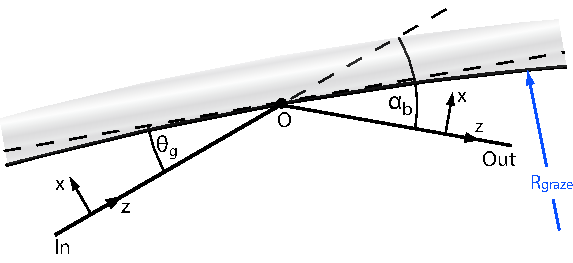
\includegraphics{mirror.pdf} 
\caption[Mirror and crystal geometry] {Mirror and crystal geometry.
The geometry shown here is appropriate for a \vn{ref_tilt} angle of
$\theta_t = 0$.  $\theta_g$ is the bend angle of the incoming
(entrance) ray, and $\alpha_b$ is the total bend
angle of the reference trajectory. A) Geometry for a mirror or a Bragg
crystal. Point $\calO$ is the origin of both the local coordinates
just before and just after the reflection/diffraction. B) Geometry for
a Laue crystal.  Point $\calO_{out}$ is the origin of the coordinates
just after diffraction is displaced from the origin $\calO_{in}$ just
before diffraction due to the finite thickness of the crystal. here
the bend angles are measured with respect to the line that is in
the plane of the entrance and exit coordinates and perpendicular to
the surface. For Laue diffraction, the user has the option of using
the undiffracted beam (shown in red) as the reference trajectory.
  }  
  \label{f:mirror}
\end{figure}

%-----------------------------------------------------------------------------
\subsection{Position Transformation When Transforming Coordinates}
\label{s:pos.trans}

A point $\bfR = (X, Y, Z)$ defined in the global coordinate system,
when expressed in the coordinate system defined by $(\bfV, \bfW)$ is
\Begineq
  \bfR_{VW} = \bfW^{-1} \left( \bfR - \bfV \right)
  \label{rwrv}
\Endeq
This is essentially the inverse of \Eq{vwlv}. That is, vectors
propagate inversely to the propagation of the coordinate system.

Using \Eq{rwrv} with \Eqs{vwlv}, and \eq{wws}, the transformation of a
particle's position $\bfr = (x,y,z)$ and momentum $\bfP = (P_x, P_y,
P_z)$ when the coordinate frame is transformed from frame
$(\bfV_{i-1}, \bfW_{i-1})$ to frame $(\bfV_i, \bfW_i)$ is
\begin{align}
  \bfr_i &= \bfS_i^{-1} \, \left( \bfr_{i-1} - \bfL_i \right), 
    \label{rwlr} \\
  \bfP_i &= \bfS_i^{-1} \, \bfP_{i-1}
    \label{pps}
\end{align}

Notice that since $\bfS$ (and $\bfW$) is the product of orthogonal
rotation matricies, $\bfS$ is itself orthogonal and its inverse is
just the transpose
\Begineq
  \bfS^{-1} = \bfS^T
\Endeq

%-----------------------------------------------------------------------------
\subsection{Crystal and Mirror Element Coordinate Transformation}
\label{s:mirror.coords}

\index{crystal}\index{mirror}\index{ref_tilt}
A \vn{crystal} element (\sref{s:mirror}) diffracts photons and a
\vn{mirror} element (\sref{s:mirror}) reflects them. For a crystal
setup for Bragg diffraction, and for a mirror, the reference orbit is
modeled as a zero length bend with $\bftilde L = (0, 0, 0)$, as shown
in \fig{f:mirror}A. Shown in the figure is the geometry
appropriate for a \vn{ref_tilt} angle of $\theta_t = 0$ (the rotation axis is
here the $y$-axis). Since the mirror or crystal element is modeled to
be of zero length, the origin points (marked $\calO$ in the figure)
of the entrance and exit local coordinates are the same. For Laue
diffraction, the only difference is that $\bftilde L$ is non-zero due
to the finite thickness of the crystal as shown in
\fig{f:mirror}B. This results in a separation between the
entrance coordinate origin $\calO_{in}$ and the exit coordinate
origin $\calO_{out}$.

In all cases, the total bending angle is
\begin{align}
  \alpha_b &= \text{bragg_angle_in} + \text{bragg_angle_out} &\text{! Crystal} \CRNO
  \alpha_b &= 2 \, \text{graze_angle}                        &\text{! Mirror}
  \label{agg}
\end{align}
With a mirror or Bragg diffraction, the bend angles are measured with
respect to the surface plane. With Laue diffraction the bend angles
are measured with respect to the line in the bend plane perpendicular
to the surface.

For Laue diffraction, the user has the option of using the
undiffracted beam (shown in red) as the reference trajectory.

The orientation of the exit coordinates (the local coordinates after
the reflection) are only affected by the element's \vn{ref_tilt} and
bend angle parameters and is independent of all other parameters such
as the radius of curvature of the surface, etc. The local $z$-axis of
the entrance coordinates along with the $z$-axis of the exit
coordinates define a plane which is called the element's \vn{bend
plane}.  For a mirror, the graze angle is a parameter supplied by the
user. For a crystal, the Bragg angles are calculated so that the
reference trajectory is in the middle of the Darwin curve. Calculation
of the Bragg angles for a crystal is given in
Section~\sref{ss:crystal.ref}.

%-----------------------------------------------------------------------------
\subsection{Element Misalignment and Origin Shift Transformation}
\label{s:patch.coords}

The \vn{Element Body} coordinates are the coordinate system attached
to an element. Without any misalignments (Here \vn{``misalignment''}
is {\em defined} to be any offset, pitch or tilt (\sref{s:offset}),
the laboratory and element body coordinates are the same. With
misalignments, the transformation is given by \Eqs{vwlv} and \eq{wws}
where 
\Begineq
  \bfL =  (\text{x_offset}, \, \text{y_offset}, \, \text{z_offset})
  \label{lxyz}
\Endeq
and the $\bfS$ matrix is defined by 
\Begineq
  \bfS = \bfW_\Theta \, \bfW_\Phi \, \bfW_\Psi
  \label{swww}
\Endeq
with
\Begineq
  \Theta = \text{x_pitch},  \qquad \Phi = \text{y_pitch},  \qquad \Psi = \text{tilt}
  \label{txppyp}
\Endeq
The form of \Eq{swww} was chosen to correspond to the form of \Eq{wwww}.

\index{patch}\index{floor_shift}
For \vn{patch} (\sref{s:patch}) and \vn{floor_shift} (\sref{s:floor.ele})
elements, the above equations are also used to calculate the the shift
in the reference coordinates from the entrance end to the exit end of
the element.

\index{rbend}\index{sbend}\index{roll}\index{tilt}
For \vn{rbend} and \vn{sbend} elements the above equations are modified
by using 
\Begineq
  \Psi = 0
\Endeq
This is used since, unlike other elements, the \vn{ref_tilt} attribute of
a bend affects the reference orbit (cf.~\Eq{ltl}). In the place of a
\vn{tilt}, the \vn{roll} attribute can be used (\sref{s:offset}). For
a \vn{roll}, the transformation at the entrance end to go from laboratory
coordinates to element coordinates is
\Begineq
  \bfL = 0, \qquad 
  \bfS = \bfW_\Theta(\text{-angle/2}) \, \bfW_\Psi(\text{roll}) \, \bfW_\Theta(\text{angle/2})
\Endeq
where \vn{angle} is the total bend angle.
The transformation back to the laboratory frame at the exit end of the bend is
\Begineq
  \bfL = 0, \qquad 
  \bfS = \bfW_\Theta(\text{angle/2}) \, \bfW_\Psi(\text{-roll}) \, \bfW_\Theta(\text{-angle/2})
\Endeq
Notice that these transformations are not inverses of one another.

\index{girder}\index{fiducial}
For \vn{fiducial} and \vn{girder} elements the above equations are
used to calculate the alignment of reference coordinates with respect
to ``\vn{origin}'' coordinates. In this case, the vector $\bfL$ is
constructed via
\Begineq
  \bfL = (\text{dx_origin}, \qquad \text{dy_origin}, \qquad \text{dz_origin})
\Endeq
And the attributes use to shift the reference coordinates orientation are:
\Begineq
  \Theta = \text{dtheta_origin}, \qquad \Phi = \text{dphi_origin}, \qquad \Psi = \text{dpsi_origin}
\Endeq

%-----------------------------------------------------------------------------
\subsection{Reflection Patch}
\label{s:reflect.patch}
\index{patch!reflection}

A \vn{Patch} (or a series of patches) that reflects the direction of
the \vn{z}-axis is called a \vn{reflection} \vn{patch}. By ``reflected
direction'' it is meant that the dot product $\Bf z_1 \cdot \Bf z_2$ is
negative where $\Bf z_1$ is the $z$-axis vector at the \vn{entrance}
face and $\Bf z_2$ is the $z$-axis vector at the \vn{exit} face. This
condition is equivalent to the condition on $\bfS$ in \Eq{swww} of
\Begineq
  S(3,3) < 0
  \label{s330}
\Endeq
Using \Eq{swww} gives after some simple algebra
\Begineq
  \cos(\text{x_pitch}) \, \cos(\text{y_pitch}) < 0
\Endeq
When there are a series of patches, The transformations of all the
patches are concatenated together to form an effective $\bfS$ which
can then be used with \Eq{s330}.

%-----------------------------------------------------------------------------
\section{Phase Space Coordinate System}
\label{s:phase.space}
\index{phase space coordinates|hyperbf}

\begin{figure}
\centering 
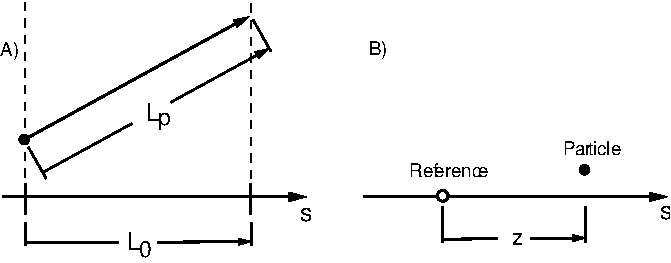
\includegraphics{canonical-z.pdf} 
\caption[Interpreting phase space $z$ at constant velocity.]
{Interpreting phase space $z$ at constant velocity: A) The change in $z$
going through an element of length $L_0$ is $L_0 - L_p$.  B) At
constant time, $z$ is the longitudinal distance between the reference
particle and the particle.}
\label{f:canonical.z}
\end{figure}

\bmad uses the phase space coordinates 
\Begineq
  \Bf r(s) = (x, p_x, y, p_y, z, p_z)
\Endeq
The longitudinal position $s$ is the independent variable instead of
the time. $x$ and $y$, are the transverse coordinates of the particle
as shown in~\fig{f:local.coords}. Note that $x$ and $y$ are independent
of the position of the reference particle.

The phase space momenta $p_x$ and $p_y$ are normalized by the
reference (sometimes called the design) momentum $P_0$
\begin{align}
  p_x = &\frac{P_x}{P_0} \CRNO
  p_y = &\frac{P_y}{P_0}
  \label{ppp}
\end{align}
where $P_x$ and $P_y$ are respectively the $x$ and $y$ momentums.


\index{lcavity}\index{rfcavity}
The phase space $z$ coordinate is 
\begin{align}
  z(s) &= -\beta(s) \, c \, (t(s) - t_0(s)) \CRNO
    &\equiv - \beta(s) \, c \, \Delta t(s)
  \label{zbctt}
\end{align}
$t(s)$ is the time at which the particle is at position $s$, $t_0(s)$
is the time at which the reference particle is at position $s$, and
$\beta$ is $v/c$ with $v$ being the particle velocity (and not the
reference velocity). The reference particle is, by definition,
``synchronized'' with elements whose fields are oscillating and therefore the
actual fields a particle will see when traveling through such an
element will depend upon the particle's phase space $z$. For example,
the energy change of a particle traveling through an \vn{lcavity} or
\vn{rfcavity} are $z$ dependent (See \sref{s:lcav} and \sref{s:rfcav}).

If the particle's velocity is constant, and is
the same as the velocity of the reference particle (for example, at
high energy where $\beta = 1$ for all particles), then $\beta \, c \,
t$ is just the path length. In this case, the change in $z$ going
through an element is
\Begineq
  \Delta z = L_0 - L_p
\Endeq
where, as shown in \fig{f:canonical.z}A, $L_0$ is the path
length of the reference particle (which is just the length of the
element) and $L_p$ is the path length of the particle in traversing
the element.  Another way of interpreting phase space $z$ is that, at
constant $\beta$, and constant time, $z$ is the longitudinal distance
between the particle and the reference particle as shown in
\fig{f:canonical.z}B. with positive $z$ indicating that the
particle is ahead of the reference particle.

Do not confuse the phase space $z$ with the $z$ that is the particle's
longitudinal coordinate in the local reference frame as shown in
\fig{f:local.coords}. By construction, this latter $z$ is
always zero.

Notice that if a particle gets an instantaneous longitudinal kick so
that $\beta$ is discontinuous then, from \Eq{zbctt}, phase space $z$ is
discontinuous even though the particle itself does not move in
space. In general, from \Eq{zbctt}, The value of $z$ for a particle at
$s_2$ is related to the value of $z$ for the particle at $s_1$ by
\Begineq
  z_2 = \frac{\beta_2}{\beta_1} \, z_1 - 
  \beta_2 \, c \, (\Delta t_2 - \Delta t_1)
  \label{zbbzb}
\Endeq
$\Delta t_2 - \Delta t_1$ can be interpreted as the difference in
transit time, between the particle and the reference particle, in going
from $s_1$ to $s_2$.

The longitudinal phase space momentum $p_z$ is given by
\begin{equation}
  p_z = \frac{\Delta P}{P_0} \equiv \frac{P - P_0}{P_0}
  \label{ppppp}
\end{equation}
where $P$ is the momentum of the particle. For ultra--relativistic particles
$p_z$ can be approximated by
\begin{equation}
  p_z = \frac{\Delta E}{E_0}
\end{equation}
\index{lcavity}
where $E_0$ is the reference energy (energy here always refers to the
total energy) and $\Delta E = E - E_0$ is the deviation of the
particle's energy from the reference energy. For an \vn{Lcavity}
element (\sref{s:lcav}) the reference momentum is {\it not} constant
so the tracking for an \vn{Lcavity} is not canonical.

\index{phase space coordinates!MAD convention}
\index{MAD!phase space convention}
\mad uses a different coordinate system where $(z, p_z)$ is
replaced by $(-c\Delta t, p_t)$ where $p_t \equiv \Delta E / P_0
c$. For highly relativistic particles the two coordinate systems are
identical.

\index{paraxial approximation}
\index{bmad_standard!tracking method}
\vn{Bmad_standard} (\sref{c:methods}) tracking and transfer matrix
calculations use the small angle (paraxial) approximation where it is
assumed that $p_x, p_y \ll 1$. With this approximation, the
relationship, between the phase space momenta and the slopes $x' \equiv
dx/ds$ and $y' \equiv dy/ds$ is
\begin{align}
  x' &\approx \frac{p_x}{1 + p_z} (1 + g x) \\
  y' &\approx \frac{p_y}{1 + p_z} (1 + g x) 
  \label{xpa1p}
\end{align}
$g = 1/\rho$ is the curvature function with $\rho$ being the radius of
curvature of the reference orbit and it has been assumed that the
bending is in the $x$--$z$ plane. 

With the paraxial approximation, and in the relativistic limit, the
change in $z$ with position is
\Begineq
  \frac{dz}{ds} = -g \, x - \frac{1}{2} (x'^2 + y'^2)
\Endeq
This shows that in a linac, without any bends, the $z$ of a particle
always decreases.

A particle can also have a spin. The spin is characterized by the
spinor $\Psi = \left( \psi_{1}, \psi_{2} \right)^{T}$ where
$\psi_{1,2}$ are complex numbers (\sref{s:spin.dyn}).

\index{phase space coordinates!PTC convention}
\index{FPP/PTC!phase space convention}
For those programmers using the PTC\index{PTC/FPP}
software package directly (ignore
this if you don't know what is being talked about here), \'Etienne Forest uses,
by default, a different coordinate system. See Chapter~\sref{c:ptc} for more details.

%-----------------------------------------------------------------------------
\section{Photon Phase Space Coordinate System}
\label{s:photon.phase.space}
\index{photon!phase space coordinates|hyperbf}

The phase space coordinates discussed above implicitly assume that
particles are traveling longitudinally in only one direction. That is,
the sign of the $s$ component of the momentum cannot be determined
from the phase space coordinates. This is generally fine for tracking
high energy beams of charged particles but for photon tracking this
would oftentimes be problematical. For photons, therefore, a different
phase space is used:
\Begineq
  (x, \beta_x, y, \beta_y, z, \beta_z)
  \label{xbybzb}
\Endeq
Here $(\beta_x, \beta_y, \beta_z)$ is the normalized photon velocity with
\Begineq
  \beta_x^2 + \beta_y^2 + \beta_z^2 = 1 
  \label{bbb1}
\Endeq
and $(x, y, z)$ are the reference orbit coordinates with $z$ being the
distance from the start of the lattice element the photon is in.

In \bmad, the information associated with a photon include its phase
space coordinates and time along with the photon energy and four
parameters $E_x, \phi_x$, and $E_y, \phi_y$ specifying the intensity
and phase of the field along the $x$ and $y$ axes transverse to the
direction of propagation.  the field in the vicinity of the photon is
\begin{align}
  E_x (\Bf r, t) &\sim E_x \, e^{i (k \, (z - z_0) - \omega \, (t - t_{ref}) + \phi_x)} \CRNO
  E_y (\Bf r, t) &\sim E_y \, e^{i (k \, (z - z_0) - \omega \, (t - t_{ref}) + \phi_y)} 
  \label{ertee}
\end{align}
where $z_0$ is the photon $z$ position and and $t_ref$ is the reference time.

The normalization between field and intensity is dependent upon the
particular parameters of any given simulation and so must be
determined by the program using \bmad.

%-----------------------------------------------------------------------------
\section{Time-based Phase Space Coordinate System}
\label{s:time.phase.space}
\index{time!phase space coordinates|hyperbf}

Some specialized routines use $(x, c p_x, y, c p_y, s, c p_s)_t$ phase
space coordinates with time $t$ as the independent variable. The
positions $x$, $y$, and $s$ are the same as in
\fig{f:local.coords}. The momenta are defined as
\begin{align}
c p_x &\equiv m c^2 \gamma \beta_x \CRNO
c p_y &\equiv m c^2 \gamma \beta_y \\
c p_s &\equiv m c^2 \gamma \beta_s, \nonumber
\end{align}
and internally are stored in units of eV.

%-----------------------------------------------------------------
\section{Relative Verses Absolute Time Tracking}
\label{s:rf.time}

\index{relative time tracking}\index{absolute time tracking}
\index{lcavity}\index{rfcavity}\index{em_field}
Unlike other elements, the kick given a particle going through an
\vn{lcavity}, \vn{rfcavity}, or possibly an \vn{em_field} element
depends upon the time that the particle enters the element relative to
some ``RF clock''. \bmad has two modes for calculating this time
called ``\vn{relative time tracking}'' and ``\vn{absolute time
tracking}''.

With \vn{relative time tracking}, which \bmad uses by default, the RF
clock is determined by the reference particle. That is, the RF phase,
\vn{phi_RF}, seen by a particle is directly related to the particles's
$z$ phase space coordinate (\sref{s:phase.space})
\begin{example}
  phi_RF = phi_particle + phi_ref
  phi_particle = -z * rf_frequency / particle_velocity
\end{example}
where \vn{phi_ref} is a fixed phase offset (generally set in the
lattice file) and independent of the particle coordinates. With
\vn{absolute time tracking}, the RF phase is simply determined by the
absolute time the particle enters the element
\begin{example}
  phi_particle = t_particle * rf_frequency
\end{example}
The switch to set the type of tracking for a lattice is
\vn{parameter[absolute_time_tracking]} (\sref{s:param}).

There are advantages and disadvantages to using either relative or
absolute time tracking. Absolute time tracking is more correct since
RF cavities are in reality synched to some clock. The problem with
absolute time tracking is that the transfer map through the cavity is
now a function of time and cannot be written as a function of $z$
unless the total lattice length is a multiple of the RF wavelength.
This complicates lattice analysis.

With relative time tracking the transfer map problem is swept under
the rug. The penelty for using relative time tracking is that results
can be unphysical. For example, the closed orbit is essentially
independent of the RF frequency. From a different angle this can be
viewed as a good feature since if one is only interested in, say,
calculating the Twiss parameters, it can be an annoyance to have to
worry that the ring one has constructed have the spacing between RF
cavities be multiples of the RF wavelength and it is potentially
confusing to see non-zero closed orbits when one is not expecting it.

The above discussion is limited to the cavity fundamental mode.
Long-range wake fields, on the other hand, cannot be synchronized to
the $z$ coordinate since, in general, their frequencies are not
commensurate with the fundamental mode frequency. For simulating the
long-range wakes, the kick is thus, by necessity, tied to the absolute
time. The exception is that a wake associated with the fundamental
mode (that is, has the same frequency as the fundamental mode) will
always use relative time if the fundamental is using relative time and
vice versa.

Do not confuse absolute time tracking with the \vn{time_runge_kutta}
tracking method (\sref{s:tkm}). The \vn{time_runge_kutta} method uses
time as the independent variable instead of $z$. Absolute time
tracking just means that the RF phase is dependent upon the time
instead of $z$. It is perfectly possible to use absolute time
tracking with code that uses $z$ as the independent variable.

\chapter{Physics}

%-----------------------------------------------------------------
\section{Units}
\label{s:units}
\index{Units|textbf}

\index{MAD!units}
\index{Units!with MAD}
\bmad uses SI (Syst\'eme International) units as shown in
Table~\ref{t:units}.  Note that \mad uses different units. For example,
\mad's unit of Particle Energy is GeV not eV.
\begin{table}[ht]
\centering
\begin{tabular}{|l|l|} \hline
  {\em Quantity}     & {\em Units}       \\ \hline
  Angles             &    radians        \\ 
  Charge             &    Coulombs       \\
  Current            &    Amps           \\ 
  Frequency          &    Hz             \\ 
  Kick               &    radians        \\ 
  Length             &    meters         \\ 
  Magnetic Field     &    Tesla          \\ 
  Particle Energy    &    eV             \\ 
  Phase Angles (RF)  &    radians/2$\pi$ \\ 
  Voltage            &    Volts          \\ \hline
\end{tabular}
\caption{Physical units used by \bmad.}
\label{t:units}
\end{table}


%-----------------------------------------------------------------
\section{Constants}
\label{s:constants}
\index{Constants|textbf}

\index{MAD}
\bmad defines commonly used physical and mathematical constants
shown in Table~\ref{t:constants}.  All symbols use straight SI units
except for \vn{e_mass} and \vn{p_mass} which are provided for
compatibility with \mad.

\begin{table}
\centering
\begin{tabular}{|l|l|l|l|} \hline
  {\em Symbol}  & {\em Value}       & {\em Units} &  {\em Name}     \\ \hline
  pi            & 3.14159265359          &        &                   \\
  twopi         & 2 * pi                 &        &                   \\
  fourpi        & 4 * pi                 &        &                   \\
  sqrt_2        & 1.4142135623731        &        &                   \\
  m_electron    & $0.51099906 \pow{6}$   & eV     & Electron mass     \\
  m_proton      & $0.938271998 \pow{9}$  & eV     & Proton mass       \\
  c_light       & $2.99792458 \pow{8}$   & m/s    & Speed of light    \\
  r_e           & $2.8179380 \pow{-15}$  & m      & Electron radius   \\
  r_p           & $1.5346980 \pow{-18}$  & m      & Proton radius     \\
  e_charge      & $1.6021892 \pow{-19}$  & C      & Electron charge   \\
  h_planck      & $6.626196 \pow{-34}$   & J/Hz   & Planck's constant \\
  h_bar_planck  & $1.054591 \pow{-34}$   & J s    & Planck / $2\pi$   \\
  e_mass        & $0.51099906 \pow{-3}$  & GeV    & Electron mass     \\
  p_mass        & $0.938271998$          & GeV    & Proton mass     \\ \hline
\end{tabular}
\caption{Physical and mathematical constants recognized by \bmad.}
\label{t:constants}
\end{table}


%-----------------------------------------------------------------
\section{Magnetic Fields}
\label{s:fields}
\index{Magnetic fields|textbf}

Start with the assumption that the local magnetic field has no
longitudinal component (obviously this assumption does not work with,
say, a solenoid).  Following \mad, the vertical magnetic field along
the $y = 0$ axis is expanded in a Taylor series
\Begineq
  B_y(x, 0) = \sum_n B_n \, \frac{x^n}{n!}
  \label{byx0b}
\Endeq
This is not the most
general form for the magnetic field. Essentially all of the skew
components have been ignored here. Assuming that the
reference orbit is locally straight (there are correction terms if the
Reference Orbit is locally curved), the field up to $3^{rd}$ order is
\begin{alignat}{5}
  B_x &=           &&B_1 y \plus         &&B_2 \, xy       && \plus && \frac{1}{6} B_3 (3x^2 y - y^3) \plus \ldots \\
  B_y &= B_0 \plus &&B_1 x + \frac{1}{2} &&B_2 (x^2 - y^2) && \plus && \frac{1}{6} B_3 (x^3 - 3x y^2) \plus \ldots
\end{alignat}
The normalized integrated multipole $K_nL$ is used when specifying magnetic
multipole components
\index{Multipole!KnL, Tn|textbf}
\Begineq
  K_nL \equiv \frac{q \, L \, B_n}{P_0}
\Endeq
$L \, B_n$ is the integrated multipole component over a length $L$,
and $P_0$ is the reference momentum. Note that $P_0/q$ is sometimes
written as $B\rho$. This is just an old notation where $\rho$ is the
bending radius of a particle with the reference energy in a field of
strength $B$. The kicks $\Delta p_x$ and $\Delta p_y$ that a
particle experiences going through a multipole field is
\begin{alignat}{5}
  \Delta p_x & = \frac{-q \, L \, B_y}{P_0} \label{pqlbp1} \\
             & = -K_0 L \;-\; 
             && K_1 L \, x \plus 
             \frac{1}{2} && K_2 L (y^2 - x^2) && \plus 
             && \frac{1}{6} K_3 L (3x y^2 - x^3) \plus \ldots 
             \nonumber \\
  \Delta p_y & = \frac{q \, L \, B_x}{P_0} \label{pqlbp2} \\
             & =     
             && K_1 L \, y \plus 
             && K_2 L \, xy && \plus 
             && \frac{1}{6} K_3L (3x^2 y - y^3) \plus \ldots \nonumber 
\end{alignat}
A positive $K_1L$ quadrupole component gives
horizontal focusing and vertical defocusing. The general form is
\begin{align}
  \Delta p_x &= \sum_{n = 0}^{\infty} \frac{K_n L}{n!} 
             \sum_{m = 0}^{\lfloor \frac{n}{2} \rfloor}
             \begin{pmatrix} n \cr 2m \end{pmatrix} \,
             (-1)^{m+1} \, x^{n-2m} \, y^{2m} \\
  \Delta p_y &= \sum_{n = 0}^{\infty} \frac{K_n L}{n!} 
             \sum_{m = 0}^{\lfloor \frac{n-1}{2} \rfloor}
             \begin{pmatrix} n \cr 2m+1 \end{pmatrix} \,
             (-1)^{m} \, x^{n-2m-1} \, y^{2m+1}
\end{align}

\index{Multipole!KnL, Tn|textbf}
So far only the normal components of the field have been
considered. If the fields associated with a particular $B_n$ multipole
component are rotated in the $(x, y)$ plane by an angle $\theta_n$, the
magnetic field at a point $(x,y)$ can be expressed in complex notation
as
\Begineq
  B_y(x,y) + i B_x(x,y) = 
    \frac{1}{n!} B_n e^{-i(n+1)\theta_n} \, e^{i n \theta} \, r^n 
  \label{bib1nb}
\Endeq
where $(r, \theta)$ are the polar coordinates of the point $(x, y)$.

\index{Multipole!an, bn|textbf}
Another representation of the magnetic field used by \bmad divides
the fields into normal $b_n$ and skew $a_n$ components. In terms of
these components the magnetic field for the $n$\Th\ order multipole is
\Begineq
  \frac{q \, L}{P_0} \, (B_y + i B_x) = (b_n + i a_n) \, (x + i y)^n
\Endeq
The conversion between $(a_n, b_n)$ and $(K_nL, \theta_n)$ is
\Begineq
  b_n + i a_n = \frac{1}{n!} \, K_nL \, e^{-i(n+1)\theta_n}
\Endeq
or
\begin{align}
  K_n L &= n! \, \sqrt{a_n^2 + b_n^2} \\
  \tan[(n+1) \theta_n] &= \frac{-a_n}{b_n}
\end{align}
To convert a normal magnet (a magnet with no skew component) into a skew
magnet (a magnet with no normal component) the magnet should be rotated
about its longitudinal axis with a rotation angle of
\Begineq
  (n+1) \theta_n = \frac{\pi}{2}
\Endeq
For example, a normal quadrupole rotated by $45^\circ$ becomes a
skew quadrupole.

\index{AB_Multipole}
\index{Radius}
When the $a_n$ and $b_n$ are associated with a physical element (as
opposed to the $a_n$ and $b_n$ associated with an \vn{AB_Multipole} element),
a measurement radius $r_0$ and a scale factor $F$ are used to scale
the $a_n$ and $b_n$ according to the formula
\Begineq
  \bigl[ a_n (\text{actual}), b_n (\text{actual}) \bigr] =
  \bigl[ a_n (\text{input}), b_n (\text{input}) \bigr] 
  \cdot F \cdot \frac{r_0^{n_\text{ref}}}{r_0^n} 
  \label{ababf}
\Endeq
$a_n(\text{input})$ and $b_n(\text{input})$ are the multipole values as given in the
lattice file. $a_n(\text{actual})$ and $b_n(\text{actual})$ are the multipole values
that are used in any simulation calculations. $r_0$ is set by the
\vn{radius} attribute of an element. $F$ and $n_\text{ref}$ are set
automatically depending upon the type of element as shown in
Table~\ref{t:ab}.

\index{AB_Multipole}
\index{Multipole}
Note that the $n = 0$ component of an \vn{AB_Multipole} or \vn{Multipole}
element rotates the reference orbit essentially acting as a zero length bend.
This is not true for multipoles that are associated with 
non-multipole elements.

\index{Kicker}
\index{Hkicker}
\index{Vkicker}
\index{Rbend}
\index{Sbend}
\index{Elseparator}
\index{Quadrupole}
\index{Solenoid}
\index{Sol_Quad}
\index{Sextupole}
\index{Octupole}
\begin{table}[ht]
\centering
\begin{tabular}{|l|l|l|} \hline
\tt
  {\em Element} & $F$                              & $n_\text{ref}$ \\ \hline
  \vn{Kicker}      & $\sqrt{{\tt Hkick}^2 + {\tt Vkick}^2}$ & 0 \\
  \vn{Hkicker}     & Kick                                   & 0 \\
  \vn{Vkicker}     & Kick                                   & 0 \\
  \vn{Rbend}       & G * L                                  & 0 \\
  \vn{Sbend}       & G * L                                  & 0 \\
  \vn{Elseparator} & $\sqrt{{\tt Hkick}^2 + {\tt Vkick}^2}$ & 0 \\
  \vn{Quadrupole}  & K1 * L                                 & 1 \\
  \vn{Solenoid}    & KS * L                                 & 1 \\
  \vn{Sol_Quad}    & K1 * L                                 & 1 \\
  \vn{Sextupole}   & K2 * L                                 & 2 \\
  \vn{Octupole}    & K3 * L                                 & 3 \\ \hline
\end{tabular}
\caption{$F$ and $n_\text{ref}$ for various elements.}
\label{t:ab}
\end{table}

%-----------------------------------------------------------------
\section{Taylor Maps}
\label{s:taylor_phys}
\index{Taylor map|textbf}

A transport map ${\cal M}: {\cal R}^6 \rightarrow {\cal R}^6$ through
an element or a section of a lattice is a function that maps the
starting phase space coordinates $\Bf r(\In)$ to the ending
coordinates $\Bf r(\Out)$
\begin{equation}
  \Bf r(\Out) = {\cal M} \, \Bf r(\In)
\end{equation}
${\cal M}$ is made up of six functions ${\cal M}_i: {\cal R}^6
 \rightarrow {\cal R}$. Each of these functions maps to one of the $r(\Out)$
coordinates. These functions can be expanded in a Taylor
series and truncated at some order. Each Taylor series is in the form
\Begineq
  r_i(\Out) = \sum_{j = 1}^N \, C_{ij} \, \prod_{k = 1}^6 \, r_k^{e_{ijk}}(\In)
  \label{rcr}
\Endeq
Where the $C_{ij}$ are coefficients and the $e_{ijk}$ are integer exponents.
The order of the map is
\Begineq
  \mbox{order} = \max_{i,j} \left( \sum_{k = 1}^6 e_{ijk} \right)
\Endeq

The standard \bmad routine for printing a Taylor map might produce something 
like this: 
\begin{example}
   Taylor Terms:
    Out     Coef              Exponents           Order        Reference
   ---------------------------------------------------
      1:     -0.600000000000  0  0  0  0  0  0        0       0.200000000
      1:      1.000000000000  1  0  0  0  0  0        1
      1:      0.145000000000  2  0  0  0  0  0        2
   ---------------------------------------------------
      2:     -0.185000000000  0  0  0  0  0  0        0       0.000000000
      2:      1.300000000000  0  1  0  0  0  0        1
      2:      3.800000000000  2  0  0  0  0  1        3
   ---------------------------------------------------
      3:      1.000000000000  0  0  1  0  0  0        1       0.100000000
      3:      1.600000000000  0  0  0  1  0  0        1
      3:    -11.138187077310  1  0  1  0  0  0        2
   ---------------------------------------------------
      4:      1.000000000000  0  0  0  1  0  0        1       0.000000000
   ---------------------------------------------------
      5:      0.000000000000  0  0  0  0  0  0        0       0.000000000
      5:      0.000001480008  0  1  0  0  0  0        1
      5:      1.000000000000  0  0  0  0  1  0        1
      5:      0.000000000003  0  0  0  0  0  1        1
      5:      0.000000000003  2  0  0  0  0  0        2
   ---------------------------------------------------
      6:      1.000000000000  0  0  0  0  0  1        1       0.000000000
\end{example}
Each line in the example represents a single taylor term. The Taylor
terms are grouped into 6 Taylor series, one each output phase space
coordinate.  The first column in the example, labeled ``out'',
(corresponding to the $i$ index in \Eq{rcr}) indicates the Taylor
series: $1 = x(out)$, $2 = p_x(out)$, etc. The 6 exponent columns give
the $e_{ijk}$ of \Eq{rcr}. In this example, the second Taylor series
(\vn{out} = 2), when expressed as a formula, would read:
\Begineq
  p_x(out) = -0.185 + 1.3 \, p_x(in) + 3.8 \, x^2(in) \, p_z(in)
\Endeq

\index{Taylor map!reference coordinates}
The reference column in the above example shows the input coordinates around
which the Taylor map is calculated. In this case, the reference
coordinates where 
\Begineq
  (x, p_x, y, p_y, z, p_z)_{ref} = (0.2, 0, 0.1, 0, 0, 0, 0)
\Endeq
The choice of the reference point will affect the values of the
coefficients of the Taylor map. For example, suppose that the exact
map through an element looks like
\Begineq
  x(out) = A \, \sin(k \, x(in))
\Endeq
Then a Taylor map to 1\St order is
\Begineq
  x(out) = c_0 + c_1 \, x(in)
\Endeq
where
\begin{align}
  c_1 &= A \, k \, \cos(k \, x_{\mbox{ref}}) \\
  c_0 &= A \, \sin(k \, x_{\mbox{ref}}) - c_1 \, x_{\mbox{ref}} \nonumber
\end{align}
Notice that once the coefficient values are determined the reference
point does not play any role when the Taylor map is evaluated to
determine the output coordinates as a function of the input
coordinates.

\index{Taylor map!feed-down}
Of importance in working with Taylor maps is the concept of
\vn{feed-down}.  This is best explained with an example. To keep the
example simple, the discussion is limited to one phase space
dimension so that the Taylor maps are a single Taylor series. Take the
map $M_1$ from point 0 to point 1 to be
\Begineq
  M_1: x_1 = x_0 + 2
  \label{xx2}
\Endeq
and the map $M_2$ from point 1 to point 2 to be
\Begineq
  M_2: x_2 = x_1^2 + 3 \, x_1
  \label{xx3x}
\Endeq
Then concatenating the maps to form the map $M_3$ from point 0 to point 2
gives
\Begineq
  M_3: x_2 = (x_0 + 2)^2 + 3 (x_0 + 2) = x_0^2 + 7 \, x_0 + 10
  \label{xx23x2}
\Endeq
However if we are evaluating our maps to only 1\St order the map $M_2$
becomes
\Begineq
  M_2: x_2 = 3 \, x_1
\Endeq
and concatenating the maps now gives
\Begineq
  M_3: x_2 = 3 (x_0 + 2) = 3 \, x_0 + 6
  \label{x3x23}
\Endeq
Comparing this to \Eq{xx23x2} shows that by neglecting the 2\Nd order
term in \Eq{xx3x} leads to 0\Th and 1\St order errors in
\Eq{x3x23}. These errors can be traced to the finite 0\Th order term in
\Eq{xx2}. This is the principal of feed--down: Given $M_3$ which is a map
produced from the concatenation of two other maps, $M_1$, and $M_2$
\Begineq
  M_3 = M_2(M_1)
\Endeq
Then if $M_1$ and $M_2$ are correct to n\Th order, $M_3$ will also be
correct to n\Th order as long as $M_1$ has no constant (0\Th order)
term. [Notice that a constant term in $M_2$ does not affect the
argument.]  What happens if we know there are constant terms in our
maps? One possibility is to go to a coordinate system where the
constant terms vanish. In the above example that would mean using the
coordinate $\widetilde x_0$ at point 0 given by
\Begineq
  \widetilde x_0 = x_0 + 2
\Endeq
\index{Symplectic integration}
The other possibility is to use symplectic integration. By its nature,
symplectic integration never has problems with feed--down.

The subject of symplectic integration is too large to be covered in
this guide. The reader is referred to the book ``Beam Dynamics: A New
Attitude and Framework'' by Etienne Forest\cite{b:forest}. A brief
synopsis: Symplectic integration uses as input 1) The Hamiltonian that
defines the equations of motion, and 2) a Taylor map $M_1$ from point 0 to
point 1. Symplectic integration from point 1 to point 2 produces a
Taylor map $M_3$ from point 0 to point 2. Symplectic integration can
produce maps to arbitrary order. In any practical application the
order $n$ of the final map is specified and in the integration
procedure all terms of order higher than $n$ are ignored. If one is
just interested in knowing the final coordinates of a particle at
point 2 given the initial coordinates at point 1 then $M_1$ is just
the constant map
\Begineq
  M_1: x_1 = c_i
\Endeq
where $c_i$ is the initial starting point. The order of the
integration is set to 0 so that all non--constant terms are
ignored. The final map is also just a constant map
\Begineq
  M_3: x_2 = c_f
\Endeq
If the map from point 1 to point 2 is desired then the map $M_1$ is
just set to the identity map
\Begineq
  M_1: x_1 = x_0
\Endeq
In general it is impossible to exactly integrate any non--linear
system. In practice, the symplectic integration is achieved by slicing
the interval between point 1 and point 2 into a number of (generally
equally spaced) slices. The integration is performed, slice step by
slice step. This is analogous to integrating a function by evaluating
the function at a number of points. Using more slices gives better
results but slows down the calculation. The speed and accuracy of the
calculation is determined by the number of slices and the \vn{order}
of the integrator. The concept of integrator order can best be
understood by analogy by considering the trapezoidal rule for
integrating a function of one variable:
\Begineq
  \int_{y_a}^{y_b} f(y) \, dy = 
  h \left[ \frac{1}{2} f(y_a) + \frac{1}{2} f(y_b) \right] +
  o(h^3 \, f^{(2)})
\Endeq
In the formula $h = y_b - y_a$ is the slice width. $0(h^3 \, f^{(2)})$
means that the error of the trapezoidal rule scales as the second
derivative of $f$. Since the error scales as $f^{(2)}$ this is an
example of a second order integrator. To integrate a function between
points $y_1$ and $y_N$ we slice the interval at points $y_2 \ldots y_{N-1}$
and apply the trapezoidal rule to each interval. Examples of higher
order integrators can be found, for example, in Numerical
Recipes\cite{b:nr}. The concept of integrator order in symplectic
integration is analogous. 

The optimum number of slices is determined by the smallest number that
gives an acceptable error. Integrators of higher order will generally
need a smaller number of slices to achieve a given accuracy. However,
since integrators of higher order take more time per slice step, and
since it is computation time and not number of slices which is
important, only a measurement of error and calculation time as a
function of slice number and integrator order will unambiguously give
the optimum integrator order and slice width.  In doing a timing test
it must be remembered that since the magnitude of any non-linearities
will depend upon position, the integration error will be dependent
upon the starting map $M_1$. For example, \bmad has integrators of
order 2, 4, and 6. To test them, timing tests were performed for some
wiggler elements (which have strong nonlinearities) and it was found
that in this case the 2\Nd order integrator gave the fastest computation 
time for a given accuracy.

%-----------------------------------------------------------------
\section{Symplectification}
\label{s:symp_method}
\index{Symplectic!symplectification}

If the evolution of a system can be described using a Hamiltonian then
it can be shown that the linear part of any transport map (the Jacobian)
must obey the symplectic condition. If a matrix $\Bf M$ is not symplectic,
Healy\cite{b:healy} has provided an elegant method for finding a symplectic 
matrix that is ``close'' to $\Bf M$. The procedure is as follows:
From $\Bf M$ a matrix $\bV$ is formed via
\begin{equation}
  \bV = \Bf S (\Bf I - \Bf M)(\Bf I + \Bf M)^{-1} 
  \label{e:vsimi}
\end{equation}
where $\Bf S$ is the matrix
\Begineq
  \Bf S = 
  \begin{pmatrix} 
      0 &  1 &  0 &  0 &  0 &  0 \cr
     -1 &  0 &  0 &  0 &  0 &  0 \cr
      0 &  0 &  0 &  1 &  0 &  0 \cr
      0 &  0 & -1 &  0 &  0 &  0 \cr
      0 &  0 &  0 &  0 &  0 & -1 \cr
      0 &  0 &  0 &  0 & -1 &  0 \cr
  \end{pmatrix}
  \label{s0100}
\Endeq
$\bV$ is symmetric if and only if $\Bf M$ is symplectic. In any case,
a symmetric matrix $\Bf W$ near $\bV$ can be
formed via
\begin{equation}
  \Bf W = \frac{\bV + \bV^t}{2}
\end{equation}
A symplectic matrix $\Bf F$ is now obtained by inverting \eq{e:vsimi}
\Begineq
  \Bf F = (\Bf I + \Bf S \Bf W) (\Bf I - \Bf S \Bf W)^{-1}
\Endeq

%-----------------------------------------------------------------
\section{LINAC Accelerating Cavities (Lcavity)}
\label{s:lcav_phys}

The transverse trajectory through an \vn{Lcavity} is modeled using equations
developed by Rosenzweig and Serafini\cite{b:rosenzweig} with
\Begineqs
  b_0 &= 1 \CRNO
  b_{-1} &= 1 \nonumber
\Endeqs
and all other $b_n$ set to zero.

The transport through the body (R\&S Eq.~(9)) has been modified to give the 
correct phase-space area at non ultra-relativistic energies:
\Begineq
  \begin{pmatrix}
    x \\ 
    x'
  \end{pmatrix}_f = 
  \begin{pmatrix}
    m_{11}                      & \beta_i \, m_{12} \\
    \frac{1}{\beta_f} \, m_{21} & \frac{\beta_i}{\beta_f} \, m_{22} 
  \end{pmatrix}
  \,
  \begin{pmatrix}
    x \\ 
    x'
  \end{pmatrix}_i
\Endeq
where the $m_{ij}$ are the matrix elements from R\&S Eq.~(9) and the 
$\beta$ are the standard relativistic factors. With this, the determinate 
of the matrix is $\beta_i \, \gamma_i / \beta_f \, \gamma_f$.

%-----------------------------------------------------------------
\section{Wigglers}
\label{s:wiggler_phys}

\index{Wiggler}
As discussed in \sref{s:wiggler}, \bmad \vn{Wiggler} elements are
split into two classes: map type and periodic type. The map type
\vn{Wigglers} are modeled using the method of Sagan, Crittenden, and
Rubin\cite{b:wiggler}. In this model the magnetic field is written as
a sum of terms $B_i$
\Begineq
  B(x,y,z) = \sum_i B_i(x, y, z; C, k_x, k_y, k_z, \phi_z)
\Endeq 
Each term $B_i$ is specified using five numbers: 
$(C, k_x, k_y, k_z, \phi_z)$. A term can take one of three forms: The first
form is
\begin{alignat}{4}
  B_x &= -&C &\dfrac{k_x}{k_y} & \sin(\kxx) \sinh(\kyy) \cos(\ksss) \CRNEG
  B_y &=  &C &                 & \cos(\kxx) \cosh(\kyy) \cos(\ksss) \CRNEG
  B_s &= -&C &\dfrac{k_s}{k_y} & \cos(\kxx) \sinh(\kyy) \sin(\ksss) \CRneg
  & \makebox[1pt][l]{with $k_y^2 = k_x^2 + k_s^2$ .} &&&  \label{f1}
\end{alignat}
The second form is
\begin{alignat}{4}
  B_x &=  &C &\dfrac{k_x}{k_y} & \sinh(\kxx) \sinh(\kyy) \cos(\ksss) \CRNEG
  B_y &=  &C &                 & \cosh(\kxx) \cosh(\kyy) \cos(\ksss) \CRNEG
  B_s &= -&C &\dfrac{k_s}{k_y} & \cosh(\kxx) \sinh(\kyy) \sin(\ksss) \CRneg
  & \makebox[1pt][l]{with $k_y^2 = k_s^2 - k_x^2$ ,} &&&  \label{f2}
\end{alignat}
The third form is
\begin{alignat}{4}
  B_x &=  &C &\dfrac{k_x}{k_y} & \sinh(\kxx) \sin(\kyy) \cos(\ksss) \CRNEG
  B_y &=  &C &                 & \cosh(\kxx) \cos(\kyy) \cos(\ksss) \CRNEG
  B_s &= -&C &\dfrac{k_s}{k_y} & \cosh(\kxx) \sin(\kyy) \sin(\ksss) \CRneg
  & \makebox[1pt][l]{with $k_y^2 = k_x^2 - k_s^2$ .} &&& \label{f3}
\end{alignat}
The relationship between $k_x$, $k_y$, and $k_z$ ensures that
Maxwell's equations are satisfied. Since the field is given by
analytic equations, Lie algebraic techniques can be use to construct
Taylor maps to arbitrary order.

``Periodic type'' wigglers use a simplified model where the magnetic
field components are
\begin{alignat}{1}
  B_y &= \hphantom{-} B_{\max} \, \cosh(k_z \, y) \, \cos(k_z \, z) \CRNO
  B_z &= -B_{\max} \, \sinh(k_z \, y) \, \sin(k_z \, z) 
\end{alignat}
where $B_{\max}$ is the maximum field on the centerline and $k$ is
given in terms of the pole length (\vn{l_pole}) by
\Begineq
  k_z = \frac{\pi}{l_{\mbox{pole}}}
\Endeq
This type of wiggler has infinitely wide poles. With
\vn{bmad_standard} tracking and transfer matrix calculations the
vertical focusing is assumed small so averaged over a period the
horizontal motion looks like a drift and the vertical motion is
modeled as a combination focusing quadrupole and focusing octupole
giving a kick\cite{b:corbett}
\Begineq
  \frac{dp_y}{ds} = k_1 \left( y + \frac{2}{3} \, k_z^2 \, y^3 \right)
\Endeq
where
\begin{alignat}{1}
  k_1 &= \frac{-1}{2} \, \left( \frac{c \, B_{\max}}{P_0 \, (1 + p_z)} \right)^2 
\end{alignat}
with $k_1$ being the linear focusing constant. For radiation
calculations the true horizontal trajectory with $y = 0$ is needed
\Begineq
  x = \frac{\sqrt{2 \, |k_1|}}{k_z^2} \, \cos (k_z \, z)
\Endeq

%-----------------------------------------------------------------
\section{Synchrotron Radiation Damping and Excitation}
\label{s:radiation}
\index{Synchrotron radiation!damping and excitation|textbf}

Emission of synchrotron radiation by a particle can be decomposed into
two parts. The deterministic average radiation emitted produces damping
while the stochastic fluctuating part produces excitation\cite{b:jowett}.

The treatment of radiation damping by \bmad essentially follows \mad.
The average change in energy $\Delta E$ of a particle going through a
section of magnet due to synchrotron radiation is
\Begineq
  \frac{\Delta E}{E_0} = -k_d \, (1 + p_z)
\Endeq
where
\Begineq
  k_d \equiv \frac{2 \, r_e}{3} \, \gamma_0^3 \, \ave{g_0^2} \, L_p \,  
  (1 + p_z)
  \label{k2r3g}
\Endeq
$r_e$ is the classical electron radius, $L_p$ is the actual path
length, $\gamma_0$ is the energy factor of an on-energy particle, $1/g_0$
is the bending radius of an on--energy particle, and $\ave{g_0^2}$ is an
average of $g_0^2$ over the actual path.

The energy lost is given by
\Begineq
  \frac{\Delta E}{E_0} = -k_f \, (1 + p_z)
\Endeq
where
\Begineq
  k_f \equiv \left( \frac{55 \, r_e \, \hbar \, c}{24 \, \sqrt{3} \, m_e} \, 
  L_p \, \gamma_0^5 \ave{g_0^3} \right)^{1/2} \, (1 + p_z) \, \xi
  \label{k55rh}
\Endeq
$\xi$ is a Gaussian distributed random number with unit sigma and zero mean.

Using \Eqs{k2r3g} and \eq{k55rh} The total change in $p_z$ can be written as
\Begineq
  \Delta p_z = \frac{\Delta E}{E_0} = -k_E \, (1 + p_z)
\Endeq
where
\Begineq
  k_E = k_d + k_f
\Endeq
Since the radiation is emitted in the forward direction the angles
$x'$ and $y'$ are invariant which leads to the following equations for
the changes in $p_x$ and $p_y$
\begin{align}
  \Delta p_x &= -k_E \, p_x \CRNO
  \Delta p_y &= -k_E \, p_y 
\end{align}

The above formalism does not take into account the fact that radiation is 
emitted with a $1/\gamma$ angular distribution. This means that the calculated
vertical emittance for a lattice with
bends only in the horizontal plane and without any coupling elements such as
skew quadrupoles will be zero. Typically, in practice, the vertical emittance
will be dominated by coupling so this approximation is generally a good one.

%-----------------------------------------------------------------
\section{Coupling and Normal Modes}
\label{s:coupling}
\index{Normal Mode!Coupling}

The coupling formalism used by \bmad is taken from the paper of Sagan
and Rubin\cite{b:coupling}. The main equations are reproduced here.  A
one--turn map $\bfT(s)$ for the transverse two--dimensional phase space
$\bfx = (x, x', y, y')$ starting and ending at some point $s$ can be
written as
  \Begineq
    \bfT = \bfV \, \bfU \, \bfV\inv 
    , \label{tvuv}
  \Endeq 
where $\bfV$ is symplectic, and $\bfU$ is of the form
  \Begineq
    \bfU = 
    \begin{pmatrix}
      \bfA & \Bf0 \cr 
      \Bf0 & \bfB \cr
    \end{pmatrix}
    . \label{ua00b}
  \Endeq
\index{Normal Mode!a--mode}
\index{Normal Mode!b--mode}
Since $\bfU$ is uncoupled the standard Twiss analysis can be
performed on the matrices $\bfA$ and $\bfB$. The normal modes
are labeled $a$ and $b$ and if the one--turn matrix $\bfT$ is
uncoupled then $a$ corresponds to the horizontal mode and $b$
corresponds to the vertical mode. 

$\bfV$ is written in the form
  \Begineq
    \bfV = 
    \begin{pmatrix}
        \gamma \bfI & \bfC \cr 
        -\bfC^+     & \gamma \bfI \cr
    \end{pmatrix}
    , \label{vgicc1}
  \Endeq
where the symplectic conjugate is 
\index{Symplectic!conjugate}
  \Begineq
    \bfC^+ = 
    \begin{pmatrix}
       C_{22} & -C_{12} \cr 
      -C_{21} & C_{11} \cr
    \end{pmatrix}
    . \label{ccccc}
  \Endeq
Since we demand that $\bfV$ be symplectic we have the condition
  \Begineq               
    \gamma^2 + \, ||\bfC|| = 1
    , \label{gc1}
  \Endeq
and $\bfV\inv$ is given by
  \Begineq
    \bfV\inv = 
    \begin{pmatrix}
      \gamma \bfI & -\bfC \cr 
      \bfC^+ & \gamma \bfI \cr
    \end{pmatrix}
    . \label{vgicc2}
  \Endeq 
$\bfC$ is a measure of the coupling. 
$\bfT$ is uncoupled if and only if $\bfC = \Bf 0$. 

It is useful to normalize out the $\beta(s)$ variation in the the above
analysis. Normalized quantities being denoted by a bar above them. The
normalized normal mode matrix $\BAR\bfU$ is defined by
  \Begineq
    \BAR\bfU = \bfG \, \bfU \, \bfG\inv
    , \label{ugug}
  \Endeq
Where $\bfG$ is given by 
  \Begineq
    \bfG \equiv 
    \begin{pmatrix}
      \bfG_a & \Bf0 \cr 
      \Bf0 & \bfG_b
    \end{pmatrix}
    , \label{gg00g}
  \Endeq  
with 
  \Begineq
    \Bf G_a = 
    \begin{pmatrix}
      \frac{\tstyle 1}{\tstyle \sqrt{\beta_a}} & 0 \cr
      \frac{\tstyle \alpha_a}{\tstyle \sqrt{\beta_a}} & \sqrt{\beta_a}
    \end{pmatrix}
    , \label{g1b0a} 
  \Endeq
with a similar equation for $\Bf G_b$. With this definition, the corresponding
$\BAR\bfA$ and $\BAR\bfB$ (cf.~\Eq{ua00b}) are just rotation matrices.
The relationship between $\bfT$ and $\BAR\bfU$ is 
  \Begineq
    \bfT = \bfG\inv \, \BAR\bfV \, \BAR\bfU \, \BAR\bfV\inv \, \bfG
    , \label{tgvuv}
  \Endeq
where
  \Begineq
    \BAR\bfV = \bfG \, \bfV \, \bfG\inv
    . \label{vgvg}
  \Endeq
Using \Eq{gg00g}, $\BAR\bfV$ can be written in the form
  \Begineq
    \BAR\bfV = 
    \begin{pmatrix}
      \gamma \bfI & \BAR\bfC \cr -\BAR\bfC^+ & \gamma \bfI
    \end{pmatrix}
    , \label{vgicc3}
  \Endeq
with the normalized matrix $\BAR\bfC$ given by
  \Begineq
    \BAR\bfC = \bfG_a \, \bfC \, \bfG_b\inv
    . \label{cgcg}
  \Endeq

The normal mode coordinates ${\bf a} = (a, a', b, b')$ are related to
the laboratory frame via
  \Begineq
    {\bf a} = \bfV\inv \, {\bf x}
    . \label{avx}
  \Endeq 
In particular the normal mode dispersion $\bfeta_a = (\eta_a,
\eta'_a, \eta_b, \eta'_b)$ is related to the laboratory frame
dispersion $\bfeta_x = (\eta_x, \eta'_x, \eta_y, \eta'_y)$ via
  \Begineq
    {\bfeta_a} = \bfV\inv \, {\bfeta_x}
    . \label{etaavx}
  \Endeq 

%-----------------------------------------------------------------
\section{Dispersion Calculation}
\label{s:dispersion}
\index{Dispersion|textbf}

The dispersion ($\eta$) and the dispersion derivative ($\eta'$) are 
defined by the equations
\begin{align}
  \eta_x &\equiv \frac{dx}{dp_z} \CRNO
  \eta'_x &\equiv \frac{d\eta_x}{ds} = \frac{dx'}{dp_z} \CRNO
  \eta_y &\equiv \frac{dy}{dp_z} \\
  \eta'_y &\equiv \frac{d\eta_y}{ds} = \frac{dy'}{dp_z} \CRNO
  \eta_z &\equiv \frac{dz}{dp_z} \CRNO
\end{align}

The dispersion calculation is as follows: 
Let $\bf r$ be the reference orbit, in canonical coordinates,
around which the dispersion is to be calculated. 
Let $\bf M$ be the transfer matrix between two points labeled 1 and 2, and
let $\bV$ be a vector defined by the equation
\Begineq
  \Bf r_2 = \bM \, \Bf r_1 + \bV
  \label{rmrv}
\Endeq
Define the dispersion vector $\bfeta$ by
\Begineq
  \bfeta = 
  \left( 
    \eta_x, \eta'_x \, (1 + p_z), \eta_y, \eta'_y \, (1 + p_z), \eta_z, 1
  \right)
\Endeq
Then differentiating \Eq{rmrv} with respect to energy, 
the dispersion at point 2 in terms of the dispersion at point 1 is
\Begineq
  \bfeta_2 = \frac{dp_{z1}}{dp_{z2}} \left[ \bM \, \bfeta_1 \right] + \bV_\eta 
\Endeq
where
\Begineq
  \bV_\eta = \frac{dp_{z1}}{dp_{z2}} \, \frac{1}{1 + p_{z1}}
  \begin{array}{c}
    M_{12} \, p_{x1} + M_{14} \, p_{y1} \\
    M_{22} \, p_{x1} + M_{24} \, p_{y1} \\
    M_{32} \, p_{x1} + M_{34} \, p_{y1} \\
    M_{42} \, p_{x1} + M_{44} \, p_{y1} \\
    M_{52} \, p_{x1} + M_{54} \, p_{y1} \\
    M_{62} \, p_{x1} + M_{64} \, p_{y1} \\
  \end{array}
  -
  \begin{array}{c}
    0 \\
    \frac{p_{x2}}{1 + p_{z2}} \\
    0 \\
    \frac{p_{y2}}{1 + p_{z2}} \\
    0 \\
    0 
  \end{array}
\Endeq
The sixth row of the matrix equation gives $dp_{z1}/dp_{z2}$. 
Explicitly
\Begineq
  \left[ \frac{dp_{z1}}{dp_{z2}} \right]^{-1} =
  M_{66} + 
  M_{61} \, \eta_{x1} + M_{62} \, \eta'_{x1} \, (1 + p_{z1}) +
  M_{63} \, \eta_{y1} + M_{64} \, \eta'_{y1} \, (1 + p_{z1}) +
  M_{62} \, p_{x1} + M_{64} \, p_{y1}
\Endeq
For everything except \vn{RFcavity} and \vn{Lcavity} elements, 
$dp_{z1}/dp_{z2}$ is 1.



%-----------------------------------------------------------------
\section{Macroparticles}
\label{s:macro}
\index{Macroparticles|textbf}

A macroparticle\cite{b:transport_appendix} is a bundle of particles
whose distribution is assumed to be Gaussian in shape. A macroparticle
is represented by a centroid position $\bfrbar$ and a $6 \times 6$
$\bfsig$ matrix which defines the shape of the macroparticle in
phase space. $\sigma_i = \sqrt{\bfsig(i,i)}$ is the RMS sigma for the $i$\Th
phase space coordinate. For example $\sigma_z = \sqrt{\bfsig(5,5)}$.

$\bfsig$ is a real, non-negative symmetric matrix. The equation that
defines the ellipsoid at a distance of $n$--sigma from the centroid is
\Begineq
  (\bfr - \bfrbar)^t \bfsig\inv (\bfr - \bfrbar) = n
\Endeq
where the $t$ superscript denotes the transpose. Given the sigma matrix
at some point $s = s_1$, the sigma matrix at a different point $s_2$ is
\Begineq
  \bfsig_2 = \bM_{21} \, \bfsig_1 \, \bM_{21}^t
\Endeq
where $\bM_{21}$ is the Jacobian of the transport map between points
$s_1$ and $s_2$.

\index{dispersion}
The Twiss parameters can be calculated from the sigma matrix. The
dispersion is given by
\begin{align}
  \bfsig(1,6) &= \eta_x \, \bfsig(6,6) \CRNO
  \bfsig(2,6) &= \eta'_x \, \bfsig(6,6) \\
  \bfsig(3,6) &= \eta_y \, \bfsig(6,6) \CRNO
  \bfsig(4,6) &= \eta'_y \, \bfsig(6,6) \nonumber
\end{align}
Ignoring coupling for now the betatron part of the sigma matrix can be
obtained from the linear equations of motion. For example, using
\Begineq
  x = \sqrt{2 \, \beta_x \, \epsilon_x} \cos \phi_x + \eta_x \, p_z
\Endeq
Solving for the first term on the RHS, squaring and averaging over all
particles gives
\Begineq
  \beta_x \, \epsilon_x = \bfsig(1,1) - \frac{\bfsig^2(1,6)}{\bfsig(6,6)}
\Endeq
It is thus convenient to define the betatron part of the sigma matrix
\Begineq
  \bfsigb(i,j) \equiv \bfsig(i,j) - \frac{\bfsig(i,6) \, \bfsig(j,6)}{\bfsig(6,6)}
\Endeq
and in terms of the betatron part the emittance is
\Begineq
  \epsilon_x^2 = \bfsigb(1,1) \, \bfsigb(2,2) - \bfsigb^2(1,2)
\Endeq
and the Twiss parameters are
\Begineq
  \epsilon_x 
  \begin{pmatrix}
    \beta_x   & -\alpha_x \\
    -\alpha_x & \gamma_x
  \end{pmatrix} = 
  \begin{pmatrix}
    \bfsigb(1,1) & \bfsigb(1,2) \\
    \bfsigb(1,2) & \bfsigb(2,2) 
  \end{pmatrix}
\Endeq

If there is coupling the transformation between the $4\times 4$
transverse normal mode sigma matrix $\bfsig_a$ and the $4\times 4$
laboratory matrix $\bfsig_x$ is
\Begineq
  \bfsig_x = \bfV \, \bfsig_a \bfV^t
\Endeq

For tracking a relativistic charged particle bunch is modeled by dividing it
longitudinally into a series of slices. Each slice is made up of a
number of macroparticles. It is assumed that the range of the
longitudinal positions of the macroparticles of a given slice do not
overlap the ranges of the other slices.

\bmad has a routine to initialize macroparticles to mirror the initial
distribution as set--up by the LIAR program\cite{b:liar}. The
initialization is as follows: The center of a
slice will be at a longitudinal position $z_j$ given by
\Begineq
  z_j = z_b + \frac{(n_s - 2 \, j + 1) \, \sigma_z \, N_{\sigma z}}{n_s}
\Endeq
where $z_b$ the overall offset of the bunch, 
$n_s$ is the number of slices, $j = 1, \ldots,
n_s$ is the index of the slice, $\sigma_z$ is the RMS bunch length,
and $N_{\sigma z}$ is the number of $\sigma_z$ the slices go out
to. The width $dz_s$ of each slice is
\Begineq
    dz_s = \frac{2 \, \sigma_z \, N_{\sigma z}}{n_s}
\Endeq
The charge associated with each slice is, within a constant factor,
the charge contained within the region between $z_j - dz_s/2$ and $z_j
+ dz_s/2$ assuming a Gaussian distribution.  The charge of all the
slices are multiplied by a factor so that the total charge of the
slices is equal to the input bunch charge.

The initialization of the macroparticles within a slice gives all the
macroparticles the same centroid position except with differing
centroid energies. 
The sigma matrix is the same for all macroparticles and is
determined by the input Twiss parameters:
\begin{align}
  \bfsig(1,1) &= \epsilon_x \, \beta_x \CRNEG
  \bfsig(1,2) &= -\epsilon_x \alpha_x  \CRNEG
  \bfsig(2,2) &= \epsilon_x \, \gamma_x = 
      \epsilon_x \, (1 + \alpha_x^2) / \beta_x \CRNEG
  \bfsig(3,3) &= \epsilon_y \, \beta_y \\
  \bfsig(3,4) &= -\epsilon_y \alpha_b \CRNEG
  \bfsig(3,4) &= \epsilon_y \, \gamma_y = 
      \epsilon_y \, (1 + \alpha_b^2) / \beta_y \CRNEG
  \bfsig(i,j) &= 0 \quad \mbox{otherwise} \nonumber
\end{align}
The centroid energy of the $k$\Th macroparticle is
\Begineq
  E_k = E_b + \frac{(n_{mp} - 2 \, k + 1) \, \sigma_E \, N_{\sigma E}}{n_{mp}}
\Endeq
where $E_b$ is the central energy of the bunch, $n_{mp}$ is the number
of macroparticles per slice, $\sigma_E$ is the energy sigma, and
$N_{\sigma E}$ is the number of sigmas in energy that the range of
macroparticle energies cover. The charge of each macroparticle is,
within a constant factor, the charge contained within the energy
region $E_k - dE_{mp}/2$ to $E_k + dE_{mp}/2$ assuming a Gaussian
distribution where the energy width $dE_{mp}$ is
\Begineq
  dE_{mp} = \frac{2 \, \sigma_E \, N_{\sigma E}}{n_{mp}}
\Endeq
The charge of all the macroparticles is adjusted by a constant factor
so that the total charge of the macroparticles within a slice is equal
to the charge associated with the slice.

%-----------------------------------------------------------------
\section{Wakefields}
\label{s:wakefields}
\index{Wakefields}

%-----------------------------
\subsection{Short--Range Wakes}

Wakefield effects are divided into short--range (within a bunch) and
long--range (between bunches).

Only the transverse dipole and longitudinal monopole components of the
short--range wakefield are modeled. The longitudinal monopole energy
kick $dE$ for the $i$\Th macroparticle is computed from the equation
\Begineq
  \Delta p_z(i) = \frac{-e \, L}{v \, P_0} \, \left(
        \frac{1}{2}\WlS(0) \,  |q_i| +
        \sum_{j \ne i} \tWl(dz_{ij}) \, |q_j| \right)
  \label{delvp}
\Endeq
where $v$ is the particle velocity, $e$ is the charge on an electron,
$q$ is the macroparticle charge, $L$ is the cavity length, $dz_{ij}$
is the longitudinal distance between the $i$\Th and $j$\Th
macroparticles, $\WlS$ is the short--range longitudinal wakefield
function, and $\tWl$ is a modified wakefield function
\Begineq
  \tWl(dz) = 
  \begin{cases}
    \WlS(0) \cdot \frac{dz + \sigma_{zij}}{2\sigma_{zij}} & 
                                    -\sigma_{zij} < dz < \sigma_{zij} \\
    \WlS(dz)                                            & \text{otherwise}
  \end{cases}
\Endeq
$\tWl$ is used instead of $\WlS$ to avoid simulation artifacts 
is due to the discontinuity of $\WlS$ at $dz = 0$. 
$\sigma_{zij}$ is the combined macroparticle length
\Begineq
  \sigma_{zij} = \sigma_{zi} + \sigma_{zj} + \sigma_{z0}
\Endeq
where $\sigma_{zi}$ and $\sigma_{zj}$ are the longitudinal sizes for
the $i$\Th and $j$\Th particles respectively, and $\sigma_{z0}$ is a
small fudge factor needed when $\sigma_{zi} = \sigma_{zj} = 0$.

The transverse kick $\Delta p_x(i)$ for the $i$\Th macroparticle due to the 
dipole short--range transverse wakefield is modeled with the equation
\Begineq
  \Delta p_x(i) = \frac{-e \, L \, \sum_j |q_j| \, x_j \, \WtS(dz_{ij})}
                 {v \, P_0}
  \label{pelqxw}
\Endeq
There is a similar equation for $\Delta p_y(i)$. $\WtS$ is the
transverse short--range wake function. Note that the LIAR
program\cite{b:liar} uses an opposite sign here.

The wakefield functions $\WlS$ and $\WlS$ can be specified in a \bmad
lattice file using a table of wake vs $z$ or by using ``pseudo'' modes
where
\Begineq
  W(z) = \sum_i A_i \, e^{d_i z} \, \sin (k_i \, z + \phi_i)
  \label{wadzk}
\Endeq
The set of mode parameters $(A_i, d_i, k_i, \phi_i)$ are chosen to fit
the calculated wake potential. The advantage of the mode approach is that
the calculation time scales as the number of particles $N$ while the
calculation based upon a table scales as $N^2$. The disadvantage is that
initially there is an extra step in that a fit to the wake potential must
be performed to generate the mode parameter values. Furthermore, since the
transverse wake typically has a form that looks something like $\sqrt{-z}$ 
for small $z$ (small here means small in magnitude, $z$ is always negative)
a set of pseudo modes may not fit the wake function well at small $z$. 
\bmad implements a hybrid scheme where for small $z$ below some cutoff
$z_{\rm{cut}}$ the wake vs $z$ table is used and for larger $z$ the pseudo
modes are used.


%-----------------------------
\subsection{Long--Range Wakes}

Following Chao\cite{b:chao} Eq.~2.88, The long--range wakefields are
characterized by a set of cavity modes. The wake function $W$ for a
mode is given by
\Begineq
  W(z) = c \, \left( \frac{R}{Q} \right) \,\,
  e^{k z/ 2 Q} \, \sin (k \, z)
\Endeq
where the wake number $k$ is related to the mode frequency $\omega$ by
\Begineq
  k = \omega / c
\Endeq
Here $z$ is the distance behind the particle generating the wake. $z$
is negative for all particles affected by the wake so $W(z)$ is a
decaying exponential as expected.

Assuming that the macroparticle generating the wake is offset a
distance $r_w$ along the $x$--axis, A trailing macroparticle will see a kick
\begin{align}
  \Delta {\Bf p}_\perp &= 
    -C \, I_m \, W_m(z) \, m \, r^{m-1} \, \left( 
    {\bf\hat r} \cos m\theta - {\bf\hat\theta} \sin m\theta \right) \\
  &= -C \, I_m \, W_m(z) \, m \, r^{m-1} \, \left( 
    {\bf\hat x} \cos [(m-1) \theta] - 
    {\bf\hat y} \sin [(m-1)\theta] \right) \CRNO
  \Delta p_z &= -C \, I_m \, W'_m(z) \, r^m \, \cos m\theta
\end{align}
where $m$ is the order of the mode,
\Begineq
  C = \frac{e}{v \, P_0}
\Endeq
 and
\Begineq
  I_m = q_w \, r_w^m
\Endeq
with $q_w$ being the charge on the particle. Generalizing the above, a
macroparticle at $(r_w, \theta_w)$ will generate a wake
\begin{align}
  -\Delta p_x + i\Delta p_y &= C \, I_m \, 
    m \, r^{m-1} \, e^{-i m \theta_w} \, e^{i (m-1) \theta} 
    \label{ppcimr} \\
  \Delta p_z &= C \, I_m \, W'(z) \, r^m \, \cos [m(\theta - \theta_w)]
    \label{pciwr}
\end{align}
Comparing \Eq{ppcimr} to \eq{bib1nb} and using the relationship between
kick and field as given by \eq{pqlbp1} and \eq{pqlbp2} shows that
the form of the wakefield transverse kick is the same as for a
multipole of order $n = m - 1$. 

The wakefield felt by a particle is due to the wakefields generated by
all the particles ahead of it. If the wakefield kicks are computed by
summing over all leading particle, trailing particle pairs then the
computation will scale as $N^2$ where $N$ is the number of
particles. This quickly becomes computationally exorbitant. A better
solution is to keep track of the wakes in a cavity. When a particle
comes through, the wake it generates is simply added to the existing
wake. This computation scales as $N$ and makes simulations with large
number of particles practical. 

To add wakes together, the wakes must be decomposed into its
components.  Spatially there are normal and skew components and
temporally there are sin and cosine components. This gives 4
components which will be labeled $a_{\cos}$, $a_{\sin}$, $b_{\cos}$,
and $b_{\sin}$. For a mode of order $m$, a particle passing through at
a distance $z_w$ with respect to the reference particle will produce
wake components
\begin{alignat}{2}
  a_{\cos} &=  &c \, \left( \frac{R}{Q} \right) \,
    e^{-k z_w/ 2 Q} \, \cos (k \, z_w) \, I_m \, \sin(m \theta_w) \CRNO
  a_{\sin} &= -&c \, \left( \frac{R}{Q} \right) \,
    e^{-k z_w/ 2 Q} \, \sin (k \, z_w) \, I_m \, \sin(m \theta_w) 
    \label{ac2rq} \\
  b_{\cos} &= -&c \, \left( \frac{R}{Q} \right) \,
    e^{-k z_w/ 2 Q} \, \cos (k \, z_w) \, I_m \, \cos(m \theta_w) \CRNO
  b_{\sin} &=  &c \, \left( \frac{R}{Q} \right) \,
    e^{-k z_w/ 2 Q} \, \sin (k \, z_w) \, I_m \, \cos(m \theta_w) \nonumber
\end{alignat}
These are added to the existing wake components. To calculate the kick
due to wake the normal and skew components are added together
\begin{align}
  a &= e^{k z/ 2 Q} \, \left( 
    a_{\cos} \, \cos (k \, z) + a_{\sin} \, \sin (k \, z) \right) 
    \label{akz2q} \\
  b &= e^{k z/ 2 Q} \, \left(
    b_{\cos} \, \cos (k \, z) + b_{\sin} \, \sin (k \, z) \right) \nonumber 
\end{align}
Here $z$ is the distance of the particle with respect the
reference particle. In analogy to \Eq{ppcimr} and \eq{pciwr} the kick
is
\begin{align}
  -\Delta p_x + i\Delta p_y &= C \, 
    m \, (b + i a) \, r^{m-1} \, e^{i (m-1) \theta} 
    \label{ppcmbar} \\
  \Delta p_z &= C \, r^m \, \left( 
    (b' + i a') e^{i m\theta} + (b' - i a') e^{-i m\theta} \right)
\end{align}
where $a' \equiv da/dz$ and $b' \equiv db/dz$.

The above equations were developed assuming cylindrical symmetry. With
cylindrical symmetry the cavity modes are actually a pair of
degenerate modes. When symmetry is broken the modes no longer have the
same frequency. In this case one has to consider a mode's polarization
angle $\phi$. Equations \eq{akz2q} and \eq{ppcmbar} are unchanged and
in place of \Eq{ac2rq}, the contribution of a particle to a mode is
\begin{alignat}{2}
  a_{\cos} &=  &c \, \left( \frac{R}{Q} \right) \,
    e^{-k z_w/ 2 Q} \, \cos (k \, z_w) \, I_m \, \left[ 
    \sin(m \theta_w) \, \sin^2(m \phi) + 
    \cos(m \theta_w) \, \sin(m \phi) \, \cos(m\phi) \right]
    \CRNO
  a_{\sin} &= -&c \, \left( \frac{R}{Q} \right) \,
    e^{-k z_w/ 2 Q} \, \sin (k \, z_w) \, I_m \, \left[
    \sin(m \theta_w) \, \sin^2(m \phi) + 
    \cos(m \theta_w) \, \sin(m \phi) \, \cos(m\phi) \right]
    \\
  b_{\cos} &= -&c \, \left( \frac{R}{Q} \right) \,
    e^{-k z_w/ 2 Q} \, \cos (k \, z_w) \, I_m \, \left[
    \cos(m \theta_w) \, \cos^2(m \phi) + 
    \sin(m \theta_w) \, \sin(m \phi) \, \cos(m\phi) \right]
    \CRNO
  b_{\sin} &=  &c \, \left( \frac{R}{Q} \right) \,
    e^{-k z_w/ 2 Q} \, \sin (k \, z_w) \, I_m \, \left[
    \cos(m \theta_w) \, \cos^2(m \phi) + 
    \sin(m \theta_w) \, \sin(m \phi) \, \cos(m\phi) \right]
    \nonumber
\end{alignat}

Each mode is characterized by an $R/Q$, $Q$, $\omega$, and $m$. Notice
that $R/Q$ is defined so that it includes the cavity length. Thus the
long--range wake equations, as opposed to the short--range ones, do
not have any explicit dependence on $L$. 

To make life more interesting different people define $R/Q$
differently. A common practice is to define an $R/Q$ ``at the beam
pipe radius''. In this case the above equations must be modified to
include factors of the beam pipe radius.

%-----------------------------------------------------------------
\section{Synchrotron Integrals}
\label{s:synch_ints}
\index{Synchrotron radiation!integrals}

The standard formulas for the synchrotron integrals used to compute
emittances, the energy spread, etc., for a lattice assume no
coupling between the horizontal and vertical
planes\cite{b:helm,b:jowett}.  With coupling the equations need to be
generalized.

\index{dispersion}
In the general case the curvature function $\Bf G = (G_x, G_y)$, which
points away from the center of curvature of the particle's orbit (see
Figure~\ref{f:local_coords}), does not lie in the horizontal
plane. $\Bf G$ has a magnitude $G = 1/\rho$ and a positive $G_y$
indicates a downward bend in the negative $y$ direction.  Similarly
the dispersion, $\bfeta\two = (\eta_x, \eta_y)$ will not lie in the
horizontal plane. With this notation the synchrotron Integrals for the
$a$ and $b$ normal modes are:
  \Begineqs
    I_1 &=& \oint ds \, \Bf G \cdot \bfeta 
         \equiv \oint ds \, (G_x \, \eta_x + G_y \, \eta_y) \\
    I_2 &=& \oint ds \, G^2 \\
    I_3 &=& \oint ds \, G^3 \\
    I_{4a} &=& \oint ds \, \left[ G^2 \, \Bf G \cdot \bfeta\two_a + 
         \nabla G^2 \cdot \bfeta\two_a \right] \\
    I_{4b} &=& \oint ds \, \left[ G^2 \, \Bf G \cdot \bfeta\two_b + 
         \nabla G^2 \cdot \bfeta\two_b \right] \\
    I_{4z} &=& \oint ds \, \left[ G^2 \, \Bf G \cdot \bfeta\two + 
         \nabla G^2 \cdot \bfeta\two \right] \\
    I_{5a} &=& \oint ds \, G^3 \, \calh_a \\
    I_{5b} &=& \oint ds \, G^3 \, \calh_b
  \Endeqs
where $\calh_a$ is 
  \Begineq
    \calh_a = \gamma_a \, \eta_a^2 + 2 \, \alpha_a \, \eta_a \, \eta_a' + 
      \beta_a \eta_a'^2 
  \Endeq
\index{dispersion}
with a similar equation for $\calh_b$. Here $\bfeta\two_a =
(\eta_{ax}, \eta_{ay})$, and $\bfeta\two_b = (\eta_{bx}, \eta_{by})$
are the dispersion vectors for the $a$ and $b$ modes respectively in
$x$--$y$ space (these 2--vectors are not to be confused with the
dispersion 4--vectors used in the previous section). The position
dependence of the curvature function is:
  \Begineqs
    G_x(x,y) = G_{x} + x \, k_1 + y \, s_1 \CRNO
    G_y(x,y) = G_{y} + x \, s_1 - y \, k_1 
  \Endeqs
where $k_1$ is the quadrupole moment and $s_1$ is the skew--quadrupole moment.
Using this gives on--axis ($x = y = 0$)
  \Begineq
    \nabla G^2 = 2 \left( G_x k_1 + G_y s_1, \, G_x s_1 - G_y k_1 \right)
    \label{g2gkg}
  \Endeq

In a dipole a non--zero $e_1$ or $e_2$ gives a contribution to $I_4$
via the $\nabla G^2 \cdot \bfeta$ term. The edge field is modeled as a
thin quadrupole of length $\delta$ and strength $k = -\tan(e) /
\delta$. It is assumed that $\Bf G$ rises linearly within the edge field
from zero on the outside edge of the edge field to its full value on the inside 
edge of the edge field. 
Using this in \Eq{g2gkg} and integrating over the edge field gives the contribution
to $I_4$ from a non--zero $e_1$ as
  \Begineq
    I_{4z} = -\tan(e_1) \, G^2
    \left( \cos(\theta) \, \eta_x + \sin(\theta) \, \eta_y \right)
    \label{iegct}
  \Endeq
With an analogous equation for a finite $e_2$. The extension to
$I_{4a}$ and $I_{4b}$ involves using $\bfeta\two_a$ and $\bfeta\two_b$
in place of $\bfeta\two$.  In \Eq{iegct} $\theta$ is the \vn{tilt}
angle which is non--zero if the bend is not in the horizontal plane.

The above integrals are invariant under rotation of the $(x,y)$ coordinate
system and reduce to the standard equations when $G_y = 0$ as they should.

There are various parameters that can be expressed in terms of these
integrals.  The $I_1$ integral can be related to the momentum
compaction $\alpha_p$ via
  \Begineq
    I_1 = \alpha_p \, L
  \Endeq
where $L$ is the storage ring circumference. The energy loss per turn is
  \Begineq
    U_0 = \frac{2 \, r_e E_0^4}{3 \, mc^2} I_2
  \Endeq
where $E_0$ is the nominal energy and $r_e$ is the classical electron
radius (electrons are assumed here but the formulas are easily
generalized).

The damping partition numbers are
  \Begineq
    J_a = 1 - \frac{I_{4a}}{I_2} \comma \quad
    J_b = 1 - \frac{I_{4b}}{I_2} \comma \, \mbox{and} \quad \label{j1ii}
    J_z = 2 + \frac{I_{4z}}{I_2} \period
  \Endeq
Since 
  \Begineq          
    \bfeta\two_{a} + \bfeta\two_{b} = \bfeta\two
    \comma \label{eee}
  \Endeq
Robinson's theorem, $J_a + J_b + J_z = 4$, is satisfied.
Alternatively, the exponential damping coefficients per turn are
  \Begineq
    \alpha_a = \frac{U_0 \, J_a}{2 E_0} \comma \quad
    \alpha_b = \frac{U_0 \, J_b}{2 E_0} \comma \, \mbox{and} \quad
    \alpha_z = \frac{U_0 \, J_z}{2 E_0} \period
  \Endeq
The energy spread is given by
  \Begineq
    \sigma_{pz}^2 = \left( \frac{\sigma_E}{E_0} \right)^2 = 
    C_q \gamma_0^2 \frac{I_3}{2I_2 + I_{4z}}
  \Endeq
where $\gamma_0$ is the usual energy factor and 
  \Begineq
    C_q = \frac{55}{32 \, \sqrt{3}} \, \frac{\hbar}{mc} = 
    3.84 \times 10^{-13} \, \mbox{meter for electrons}
  \Endeq
If the synchrotron frequency is not too large the bunch length is given by
  \Begineq
    \sigma_z = \frac{I_1}{M(6,5)} \, \sigma_{pz}
  \Endeq
where $M(6,5)$ is the $(6,5)$ element for the 1--turn transfer matrix
of the storage ring. Finally the emittances are given by
  \Begineqs
    \epsilon_a \AND= C_q \, \gamma_0^2 \frac{I_{5a}}{I_2 - I_{4a}} \CRNO
    \epsilon_b \AND= C_q \, \gamma_0^2 \frac{I_{5b}}{I_2 - I_{4b}}
  \Endeqs

For a linac radiation integrals are still of interest if there are
bends but in this case the appropriate energy factors must be included
to take account the changing energy in the line. $I_1$ is not altered and
the $I_4$ integrals are not relevant. The other integrals become
  \Begineqs
    L_2 &=& \int ds \, G^2 \, \gamma_0^4 \\
    L_3 &=& \int ds \, G^3 \, \gamma_0^7 \\
    L_{5a} &=& \int ds \, G^3 \, \calh_a \, \gamma_0^6 \\
    L_{5b} &=& \int ds \, G^3 \, \calh_b \, \gamma_0^6
  \Endeqs
In terms of these integrals the energy loss through the linac is
  \Begineq
    U_0 = \frac{2 \, r_e \, mc^2}{3} L_2
  \Endeq
The energy spread assuming $\sigma_E$ is zero at the start and neglecting
any damping is
  \Begineq
    \sigma_E^2 = \frac{4}{3} \, C_q \, r_e \, \left( m c^2 \right)^2 \, L_3
  \Endeq
and, again neglecting any initial beam width, the transverse beam size
at the end of the linac is
  \Begineqs
    \epsilon_a \AND= \frac{2}{3} \, C_q \, r_e \, 
    \frac{L_{5a}}{\gamma_f} \CRNO
    \epsilon_b \AND= \frac{2}{3} \, C_q \, r_e \, 
    \frac{L_{5b}}{\gamma_f} 
  \Endeqs
Where $\gamma_f$ is the final gamma

%-----------------------------------------------------------------   
 \section{Spin Dynamics}   
 \label{s:spin_dyn}   
 \index{Spin tracking!Spin dynamics}   
    
 The matrix representation of the observable corresponding to the measurement of   
 spin along the unit vector $\Bf u$ in the ${ |+> = \left(\begin{matrix}1 \\ 0   
 \end{matrix} \right), |-> =  \left(\begin{matrix} 0 \\ 1 \end{matrix} \right) }$ 
basis is   
   \Begineqs   
     S_{\Bf u} &=& \mathbf{S \cdot u} \\   
               &=& \frac{\hbar}{2} \sigma_{x} \sin \theta \cos \phi +   
                   \frac{\hbar}{2} \sigma_{y} \sin \theta \sin \phi +   
                   \frac{\hbar}{2} \sigma_{z} \cos \theta \\   
               &=& \frac{\hbar}{2} \left(   
                    \begin{matrix}   
                      \cos \theta            & \sin \theta e^{- i \phi} \\   
                      \sin \theta e^{i \phi} & - \cos \theta   
                    \end{matrix} \right)   
   \Endeqs   
 where $\theta$ and $\phi$ are the polar angles characterizing the vector $\Bf u$   
 and $\sigma_{x,y,z}$ are the three pauli matrices.   
 The expectation value of this operator representing the spin of a particle   
 satisfies the equation of motion of a classical spin vector in the particle's   
 instantaneous rest frame. The classical spin vector $\Bf s$ is described for   
 time $t$ in the   
 laboratory frame by the Thomas-Bargmann-Michel-Telegdi (T-BMT) equation,   
   \Begineqs   
     \frac{\mathrm{d}}{\mathrm{d}t} \Bf s &=& {\pmb\Omega}_{BMT} (\mathbf{r,p,t})   
     \mathbf{ \times  s}, \\   
             \Omega_{BMT}(\mathbf{r,p,t}) &=& - \frac{q}{m \gamma} \left[\left(1   
             + G \gamma \right) \Bf B - \frac{G \Bf p \cdot \Bf B}{\left( \gamma   
             + 1\right) m^{2} c^{2}} \Bf p - \frac{1}{m c^{2}}\left(G +   
             \frac{1}{1 + \gamma}\right)\mathbf{ p \times  E}\right],   
   \Endeqs   
 where $\Bf E (\Bf r ,t)$ and $\Bf B (\Bf r ,t)$ are the electric and magnetic   
 fields in the laboratory frame, $\Bf p$ and $\gamma$ are the particle's momentum   
 and relativistic gamma factor in the laboratory frame, $q$ and $m$ are the   
 particle's charge and mass, and $G = \frac{\left(g-2\right)}{2}$ is the   
 particle's anaomalous gyro-magnetic g-factor which is $1.793$ for protons and   
 $0.00116$ for electrons and positrons.   
    
 For a distribution of spins the polarization $P$ along the unit vector $\Bf u$ is
 defined as the absolute   
 value of the average expectation value of the spin over all N particles times   
 $\frac{2}{\hbar}$,   
   \Begineqs   
     P &=& \frac{2}{\hbar} \| \frac{1}{N} \sum_{j=1}^{N}<+|S_{\Bf u}|+> \| \\   
       &=& \| \frac{1}{N} \sum_{j=1}^{N} \cos \theta \|.   
   \Endeqs   
    
 It is more efficient to use the SU(2) representation rather than SO(3) when   
 describing rotations of spin. In the SU(2) representation, a spin $\Bf s$ is   
 written as a spinor $\Psi = \left( \psi_{1}, \psi_{2} \right)^{T}$ where   
 $\psi_{1,2}$ are complex numbers and   
   \Begineqs   
                     \Bf s &=& \Psi^{\dagger} \Bf \sigma \Psi \\   
     \leftrightarrow \Psi  &=& \frac{1}{\sqrt{2 \left(s_{3}+1\right)}}   
              \left( \begin{matrix} 1+s_{3} \\ s_{1}+i s_{2} \end{matrix}   
              \right),   
   \Endeqs   
 or in polar coordinates,   
   \Begineqs   
     \Psi &=& \left( \begin{matrix} \psi_{1} \\ \psi_{2} \end{matrix} \right)   
          = e^{i \xi} \left( \begin{matrix} \cos \frac{\phi}{2}\\   
                      \sin \frac{\phi}{2} e^{i \phi}   
                      \end{matrix} \right) \\   
          \leftrightarrow   
     \Bf s &=& \left( \begin{matrix} \sin \theta \cos \phi \\   
                                     \sin \theta \sin \phi \\   
                                     \cos \theta \end{matrix} \right).   
   \Endeqs   
 The $\xi$ being an extra phase factor. Due to the unitarity of the spin vector,   
 $|\psi_{1}|^{2} + |\psi_{2}|^{2} = 1$.   
    
 In spinor notation the T-BMT equation can be written   
   \Begineq   
     \frac{\mathrm{d}}{\mathrm{d} t} \Psi = - \frac{i}{2} \left( \Bf \sigma \cdot   
     {\pmb\Omega} \right) \Psi.   
   \Endeq   
 The solution leads to a rotation of the spin vector by an angle   
 $\alpha$ around a unit vector $\Bf e$ represented as   
   \Begineqs   
     \Psi &=& e^{-i \frac{\alpha}{2} \Bf e \cdot \Bf \sigma} \Psi_{i} \\   
          &=& \left( a_{0} \Bf 1_{2} - i \boldsymbol{a} \cdot \Bf \sigma \right) \Psi_{i} \\   
          &=& \Bf A \Psi_{i}.   
   \Endeqs   
 The SU(2) matrix $\Bf A$ is called a \textit{quaternion} and has the   
 normalization condition $a_{0}^{2} + \boldsymbol{a}^{2} = 1$. The three components   
 $\left(a_{1}, a_{2}, a_{3}\right)$, along with the normalization condition,   
 describes the transport of spin between any two points in an accelerator. 
 
% LocalWords: rcr


%----------------------------------------------------------------
\part{Language Reference}
%----------------------------------------------------------------
\chapter{Lattice File Overview}
\index{lattice files|hyperbf}

\index{Bmad!lattice file format}
A lattice defines
the sequence of elements that a particle will travel
through along with the attributes (length,
strength, orientation, etc.) of the elements. 
A lattice file (or files) is a file that is used to describe an 
accelerator or storage ring. 
The \bmad software library comes with
routines to parse lattice files. There are two input formats
that \bmad understands: The \bmad standard format and
XSIF\cite{b:xsif}. XSIF, developed at SLAC,
has its own documentation and will not be discussed in detail
here except for a few brief notes in Section~(\sref{s:xsif}). 
Throughout this manual, unless explicitly stated otherwise,
the lattice format under discussion will always pertain to the \bmad
standard format. 

While \bmad cannot directlhy read in \mad\cite{b:mad.user} files, 
translation between \mad and \bmad lattice files is possible using
the \vn{Universal Accelerator Parser} as disscused in Section~\sref{s:aml}.

%---------------------------------------------------------------------------
\section{Lattice File Format}
\label{s:lattice.file.formats}

\index{MAD!lattice format}
The syntax that a \bmad standard lattice file must conform to is
modeled after the lattice input format of the \mad program.
Essentially, a \bmad lattice file is similar to a \mad lattice file
except that a \bmad file has no ``action'' commands (action commands
tell the program to calculate the Twiss parameters, do tracking,
etc.).  Since \bmad is a software library, interacting with the user to 
determine what actions a program
should take is left to the program and is not part of \bmad (although
the \bmad library provides the routines to perform many of the standard
calculations). A program is not required to use the \bmad parser
routines but, if it does, the following chapters describe how to
construct a valid lattice file.

%---------------------------------------------------------------------------
\section{File Example and Syntax}
\index{Bmad!statement syntax}

\index{parameter statement}
\index{use statement}
The following (rather silly) example shows some of the features of a
\bmad lattice file:
\begin{example}
  ! This is a comment
  parameter[E_TOT] = 5e9                   ! Parameter definition
  pa1 = sin(3.47 * pi / c_light)                 ! Constant definition
  bend1: sbend, type = "arc bend", l = 2.3,      ! An element definition
      g = 2*pa1, tracking_method = bmad_standard
  bend2: bend1, l = 3.4                          ! Another element def
  bend2[g] = 105 - exp(2.3) / 37.5               ! Redefining an attribute
  ln1: line = (ele1, ele2, ele3)                 ! A line definition
  ln2: line = (ln1, ele4, ele5)                  ! Lines can contain lines
  arg_ln(a, b) = (ele1, a, ele2, b)              ! A line with arguments.
  use, ln2                                       ! Which line to use for the lattice
\end{example}

\index{"! comment symbol}
\index{comment symbol ("!)}
A \bmad lattice file consists of a sequence of statements. An
exclamation mark (!) denotes a comment and the exclamation mark and
everything after the exclamation mark on a line are ignored.  \bmad is
generally case insensitive. All names are converted to uppercase
except strings (\sref{s:var.types}). Exceptions where a name is not
converted include file names and atomic formulas for materials used in
crystal diffraction.

\index{\& continuation symbol}
\index{continuation symbol (\&)}
Normally a statement occupies a single line in the file. Several
statements may be placed on the same line by inserting a semicolon
(``;'') between them. A long statement can occupy multiple lines by
putting an ampersand (``\&'') at the end of each line of the statement
except for the last line. Additionally, lines that end with an
``implicit continuation character''
are automatically continued to the next line. The implicit continuation 
characters are
\begin{example}
  ,   +   -   *   /   (   \{   [   =
\end{example}
Notice
that this is {\em not} like \vn{C/C++}. Thus the following is bad syntax
\begin{example}
  wall = \{
    section = \{s = 0.45     ! BAD SYNTAX. NO CONTINUATION CHARACTER HERE.
    \}                       ! BAD SYNTAX. NO CONTINUATION CHARACTER HERE.
  \}
\end{example}
Correct is:
\begin{example}
  wall = \{
    section = \{s = 0.45\} \}
\end{example}
or even:
\begin{example}
  wall = \{
    section = \{s = 0.45\} \&
  \}
\end{example}

\index{lattice files!name syntax}
Names of constants, elements, lines, etc. are limited to 40
characters. The first character must be a letter (\vn{A} --- \vn{Z}).
The other characters may be a letter, a digit (\vn{0} --- \vn{9}) or
an underscore (\vn{_}). Other characters may appear but should be avoided
since they are used by Bmad for various purposes. For example, the 
backslash (\vn{\B}) character is used to by Bmad when forming the names of
superposition slaves (\sref{s:super}) and dots (\vn{.}) are used by Bmad 
when creating names of \vn{tagged} elements (\sref{s:tag}). Also use of
special characters may make the lattice files less portable to non-Bmad programs.

\index{parameter statement}
\index{parameter statement}
\index{parameter statement}
\index{beginning statement}
The following example constructs a linear lattice with two elements: 
\begin{example}
  parameter[lattice_type] = LINEAR_LATTICE
  parameter[e_tot] =2.7389062E9
  parameter[particle] = POSITRON
  beginning[beta_a] = 14.5011548
  beginning[alpha_a] = -0.53828197
  beginning[beta_b] = 31.3178048
  beginning[alpha_b] = 0.25761815
  q: quadrupole, l = 0.6, b1_gradient = 9.011
  d: drift, l = 2.5
  t: line = (q, d)
  use, t 
\end{example}
here \vn{parameter[lattice_type]} (\sref{s:param}) is set to \vn{LINEAR_LATTICE}
which specifies that the lattice is not circular. In this case, the beginning 
Twiss parameters need to be specified and this is done by the \vn{beginning}
statements (\sref{s:beginning}). A quadrupole named \vn{q}
and a drift element named \vn{d} are specified
and the entire lattice consists of element \vn{q} followed by element \vn{d}.

%----------------------------------------------------------------------------
\section{Digested Files}
\label{s:lattice.files}
\index{digested files}

Normally the \bmad parser routine will create what is called a
``digested file'' after it has parsed a lattice file so that when a
program is run and the same lattice file is to be read in again, to save
time, the digested file can be used to load in the lattice information.
This digested file is in binary format and is not human readable. The
digested file will contain the transfer maps for all the elements. 
Using a digested file can save considerable time if some of the
elements in the lattice need to have Taylor maps computed.
(this occurs typically with map--type wigglers).

\bmad creates the digested file in the same area as the lattice file.
If \bmad is not able to create a digested file (typically because it
does not have write permission in the directory), an error message will
be generated but otherwise program operation will be normal.

\index{ran}
\index{ran_gauss}
Digested files contain the names of the lattice files used to create
them. If a lattice file has been modified since the digested file has
been created then the lattice files will be reread and a new
digested file will be generated. 

Note: If any of the random number functions (\sref{s:functions}) are
used in the process of creating the lattice, the digested file will be
ignored. In this case, each time the lattice is read into a program,
different random numbers will be generated for expressions that use such
random numbers.

Digested files can also be used for easy transport of lattices between
programs or between sessions of a program. For example, using one
program you might read in a lattice, make some adjustments (say to model
shifts in magnet positions) and then write out a digested version of the
lattice. This adjusted lattice can now be read in by another program.

%---------------------------------------------------------------------------
\section{Element Sequence Definition}

\index{line}\index{use statement|hyperbf}
A \vn{line} defines a sequence of elements. \vn{lines} may contain
other \vn{lines} and so a hierarchy may be established. One line is
selected, via a \vn{use} statement, that defines the lattice. For
example:
\begin{example}
  l3: line = (l1, l2)   ! Concatenate two lines
  l1: line = (a, b, c)  ! Line with 3 elements
  l2: line = (a, z)     ! Another line 
  use, l3               ! Use l3 as the lattice definition.
\end{example}
In this case the lattice would be
\begin{example}
  (a, b, c, a, z)
\end{example}
\vn{Lines} can be defined in any order. See \cref{c:sequence} for more
details.

\index{superimpose}
The \vn{superimpose} construct allows elements to be placed in a
lattice at a definite longitudinal position. What happens is that
after a lattice is expanded, there is a reshuffling of the elements to
accommodate any new superimpose elements. See \sref{s:super} for more
details.

%---------------------------------------------------------------------------
\section{Lattice Elements}

The syntax for defining a lattice element roughly follows the
\mad\cite{b:maduser} program:
\begin{example}
  ele_name: keyword [, attributes]
\end{example}
where \vn{ele_name} is the element name, \vn{keyword} is the type of
element, and \vn{attributes} is a list of the elements
attributes. \cref{c:elements} gives a list of elements types with
their attributes.
\vn{Overlay} and \vn{group} type elements have a slightly different syntax:
\begin{example}
  ele_name: keyword = \{ list \}, master-attribute [= value] [, attributes]
\end{example}
and \vn{Girder} elements have the syntax
\begin{example}
  ele_name: keyword = \{ list \} [, attributes]
\end{example}  
For example:
\begin{example}
  q01w: quadrupole, type = "A String", l = 0.6, tilt = pi/2
  h10e: overlay = \{ b08e, b10e \}, hkick
\end{example}


%---------------------------------------------------------------------------
\section{Lattice Element Names}
\label{s:ele.names}
\index{element!names}

\index{element!name}\index{superimpose}\index{multipass}
A valid element name may be up to 40 characters in length. The first
character of the name must be a letter [A-Z]. After that, the rest of
the name can contain only letters, digits [0-9], underscore ``_'',
period ``.'', backslash ``\B'', or a hash mark ``\#''. It is best to
avoid these last three symbols since \bmad uses them to denote
``relationships''.  Periods are used for tagging (\sref{s:tag}), and
backslash and hash marks are used for to compose names for
superposition (\sref{s:super}) and multipass (\sref{s:multipass})
slave elements.

\index{reserved names}
\index{beam}\index{beam_start}\index{beginning}
\index{end}\index{parameter}\index{root}
There is a short list of names that cannot be used as an element name. 
These reserved names are:
\begin{example}
  BEAM
  BEAM_START
  BEGINNING
  END
  PARAMETER
  ROOT
\end{example}

%---------------------------------------------------------------------------
\section{Lattice Element Attributes}
\label{s:lat.attribs}
\index{element attribute|hyperbf}

Any lattice element has various attributes like its name, its length,
its strength, etc. The values of element attributes can be specified
when the element is defined. For example:
\begin{example}
  b01w: sbend, l = 6.0, rho = 89.0 ! Define an element with attributes.
\end{example}
After an element's definition, an individual attribute may be referred
to using the syntax
\begin{example}
  element-name[attribute-name]
\end{example}
Element attributes can be set or used in an algebraic expression:
\begin{example}
  bo1w[roll] = 6.5                  ! Set an attribute value.
  b01w[l] = 6.5                     ! Change an attribute value.
  b01w[l] = b01w[rho] / 12          ! OK to reset an attribute value.
  my_const = b01w[rho] / b01w[l]      ! Use of attribute values in an expression.
\end{example}
Notice that there can be no space between the element name and the
\vn{[} opening bracket.  

When setting an attribute value, if more than one element has the
\vn{element-name} then {\it all} such elements will be set.  When
setting an attribute value, if \vn{element-name} is the name of a type
of element, all elements of that type will be set. For example
\begin{example}
  q_arc[k1] = 0.234                      ! Set all elements named Q_ARC. 
  rfcavity[voltage] = 3.7                ! Set all RFcavity elements.
\end{example}

With element attribute sets, The wild cards \vn{``*''},
and \vn{``\%''} can be used to can be used where \vn{``*''} denotes
any number of characters and \vn{``%''} denotes a single character. Examples:
\begin{example}
  *[tracking_method] = bmad_standard  ! Matches all elements.
  Q*[k1] = 0.234                      ! Matches all elements with names beginning with Q.
  Q%1[k1] = 0.234                     ! Matches to "Q01" but not "Q001".
\end{example}
\index{beginning element}
Note: A name with wild cards will never match to the \vn{BEGINNING} element (\sref{s:use}).

After lattice expansion (\sref{s:expand}), The element index can be
used to in element attribute sets. The element index is 1 for the
first element in the lattice, etc. Example:
\begin{example}
  expand_lattice          ! Expand the lattice.
  97[x_offset] = 0.0023   ! Set x_offset attribute of 97th element
  ... etc ...
\end{example}
Generally using the element index should be avoided but it can be
useful when dealing with a lattice where multiple elements share the
same name.

\cref{c:elements} gives a list of elements with their attributes.

Multiple elements in a lattice may share the same name.  When
branching (\sref{s:branching}) is used, to differentiate elements that
appear in different branches, the ``branch qualified'' element name may be
used. The branch qualified element name is of the form
\begin{example}
  branch_name>>element_name
\end{example}
where \vn{branch_name} is the name of the branch and \vn{element_name}
is the ``regular'' name of the element. Example:
\begin{example}
  root>>q10w
  x_branch>>crystal3
\end{example}

%---------------------------------------------------------------------------
\section{Variable Types}
\label{s:var.types}
\index{arithmetic expressions!variables}

\index{logicals|hyperbf}
There are five types of variables in \bmad: reals, integers, switches,
logicals (booleans), and strings. Acceptable logical values are
\begin{example}
   true    false
   t       f
\end{example}
For example
\begin{example}
  rf1[is_on] = False
\end{example}

\index{strings|hyperbf}
String literals can be quoted using double quotes (") or single quotes ('). 
If there are no
blanks or commas within a string, the quotes can be omitted. For example:
\begin{example}
  Q00W: Quad, type = "My Type", alias = Who_knows, &
                                  descrip = "Only the shadow knows"
\end{example}
Unlike most everything else, strings are not converted to uppercase.

\index{switches|hyperbf}
Switches are variables that take discrete values. For example:
\begin{example}
  parameter[particle] = positron          
  q01w: quad, tracking_method = bmad_standard 
\end{example}
The name ``switch'' can refer to the variable (for example,
\vn{tracking_method}) or to a value that it can take (for example,
\vn{bmad_standard}). The name ``method'' is used interchangeably with switch.

%-----------------------------------------------------------------
\section{Units and Constants}
\label{s:constants}
\index{constants|hyperbf}

\bmad uses SI (Syst\'eme International) units as shown in
Table~\ref{t:units}.

\bmad defines commonly used physical and mathematical constants
shown in Table~\ref{t:constants}.  All symbols use straight SI units
except for \vn{e_mass} and \vn{p_mass} which are provided for
compatibility with \mad.

\begin{table}
\centering
\begin{tabular}{|l|l|l|l|} \hline
  {\em Symbol}  & {\em Value}       & {\em Units} &  {\em Name}       \\ \hline
  pi            & 3.14159265359          &        &                   \\
  twopi         & 2 * pi                 &        &                   \\
  fourpi        & 4 * pi                 &        &                   \\
  e_log         & 2.718281828            &        &                   \\
  sqrt_2        & 1.4142135623731        &        &                   \\
  degrees       & 180 / pi               &        &                   \\
  m_electron    & $0.51099906 \pow{6}$   & eV     & Electron mass     \\
  m_muon        & $0.1056583893 \pow{6}$ & eV     & Muon mass         \\
  m_proton      & $0.938271998 \pow{9}$  & eV     & Proton mass       \\
  c_light       & $2.99792458 \pow{8}$   & m/sec  & Speed of light    \\
  r_e           & $2.8179380 \pow{-15}$  & m      & Electron radius   \\
  r_p           & $1.5346980 \pow{-18}$  & m      & Proton radius     \\
  e_charge      & $1.6021892 \pow{-19}$  & C      & Electron charge   \\
  h_planck      & $4.13566733 \pow{-15}$ & eV*sec & Planck's constant \\
  h_bar_planck  & $6.58211899 \pow{-16}$ & eV*sec & Planck / $2\pi$   \\
  e_mass        & $0.51099906 \pow{-3}$  & GeV    & Electron mass     \\
  p_mass        & $0.938271998$          & GeV    & Proton mass       \\ \hline
\end{tabular}
\caption{Physical and mathematical constants recognized by \bmad.}
\label{t:constants}
\end{table}

%---------------------------------------------------------------------------
\section{Arithmetic Expressions}
\index{arithmetic expressions} 

Arithmetic expressions can be used in a place where a real value is required.
The standard operators are defined: \hfil\break
\hspace*{0.15in}
\begin{tabular}{ll}
  $a + b$           & Addition        \\
  $a - b$           & Subtraction     \\
  $a \, \ast \, b$  & Multiplication  \\
  $a \; / \; b$     & Division        \\
  $a \, \land \, b$ & Exponentiation  \\
\end{tabular}
\hfil\break
\bmad also has a set of intrinsic functions. A list of these is given
in \sref{s:functions}.

\index{arithmetic expressions!constants}
Literal constants can be entered with or without a decimal point. An
exponent is marked with the letter E. For example
\begin{example}
  1, 10.35, 5E3, 314.159E-2
\end{example}
Symbolic constants can be defined using the syntax
\begin{example}
  parameter_name = expression
\end{example}
\index{MAD!syntax compatibility with BMAD}
Alternatively, to be compatible with \mad, using ``:='' instead of ``='' is accepted
\begin{example}
  parameter_name := expression
\end{example}
Examples:
\begin{example}
  my_const = sqrt(10.3) * pi^3
  abc     := my_const * 23
\end{example}
\index{MAD!delayed substitution}
Unlike \mad, \bmad uses immediate substitution so that all constants
in an expression must have been previously defined. For example, the
following is not valid:
\begin{example}
  abc      = my_const * 23      ! No: my_const needs to be defined first.
  my_const = sqrt(10.3) * pi^3
\end{example}
here the value of \vn{my_const} is not known when the line ``\vn{abc}
= $\ldots$'' is parsed. Once
defined, symbolic constants cannot be redefined. For example:
\begin{example}
  my_const = 1
  my_const = 2  ! No: my_const cannot be redefined.
\end{example}

%---------------------------------------------------------------------------
\section{Intrinsic functions}
\label{s:functions}
\index{intrinsic functions}

\index{sqrt}\index{log}\index{exp}\index{sin}\index{cos}\index{tan}
\index{asin}\index{acos}\index{atan}\index{abs}\index{ran}\index{ran_gauss}
The following intrinsic functions are recognized by \bmad: \hfil\break
\hspace*{0.15in}
\begin{tabular}{ll}
  \vn{sqrt}(x)      & Square Root    \\
  \vn{log}(x)       & Logarithm      \\
  \vn{exp}(x)       & Exponential    \\
  \vn{sin}(x)       & Sine           \\
  \vn{cos}(x)       & Cosine         \\
  \vn{tan}(x)       & Tangent        \\
  \vn{asin}(x)      & Arc sine       \\
  \vn{acos}(x)      & Arc cosine     \\
  \vn{atan}(x)      & Arc Tangent    \\
  \vn{abs}(x)       & Absolute Value \\
  \vn{ran}()        & Random number between 0 and 1 \\
  \vn{ran_gauss}()  & Gaussian distributed random number \\
\end{tabular}

\index{ran_seed}
\vn{ran_gauss} is a Gaussian distributed random number with unit RMS. 
Both \vn{ran} and \vn{ran_gauss} use a seeded random number generator. 
To choose the seed set 
\begin{example}
  parameter[ran_seed] = <Integer>
\end{example}
A \vn{value} of zero will set the seed using the system clock so that
different sequences of random numbers will be generated each time a
program is run.  The default behavior if \vn{parameter[ran_seed]} is
not present is to use the system clock for the seed.

\index{expand_lattice}
If an element is used multiple times in a lattice, and if \vn{ran} or
\vn{gauss_ran} is used to set an attribute value of this element, then
to have all instances of the element have different attribute values
the setting of the attribute must be after the lattice has been
expanded (\sref{s:expand}). For example:
\begin{example}
  a: quad 
  a[x_offset] = 0.001*ran_gauss()
  my_line: line = (a, a)
  use, my_line
\end{example}
Here, because \bmad does immediate evaluation, the \vn{x_offset}
values for \vn{a} gets set in line 2 and so both copies of \vn{a} in
the lattice get the same value. This is probably not what is wanted.
On the other hand if the attribute is set after lattice expansion:
\begin{example}
  a: quad 
  my_line: line = (a, a)
  use, my_line
  expand_lattice
  a[x_offset] = 0.001*ran_gauss()
\end{example}
Here the two \vn{a} elements in the lattice get different values for
\vn{x_offset}.

%-----------------------------------------------------------------------------
\section{Title Statement}
\index{title statement|hyperbf}

The \vn{title} statement sets a title string which can be used by a program. 
For consistency with \mad there are two possible syntaxes
\begin{example}
  title, <String>
\end{example}
or the statement can be split into two lines
\begin{example}
  title
  <String>
\end{example}
For example
\begin{example}
  title
  "This is a title"
\end{example}

%--------------------------------------------------------------------------
\section{Call Statement}
\label{s:call}
\index{call statement|hyperbf}

It is frequently convenient to separate the lattice definition into
several files.  Typically there might be a file (or files) that define
the layout of the lattice (something that doesn't change often) and a
file (or files) that define magnet strengths (something that changes
more often).  The \vn{call} is used to read in separated lattice
files. The syntax is
\begin{example}
  call, filename = <String>
\end{example}
Example:
\begin{example}
  call, filename = "../layout/my_layout.bmad"      ! Relative pathname
  call, filename = "/nfs/cesr/lat/my_layout.bmad"  ! Absolute pathname
\end{example}
\bmad will read the called file until a \vn{return} or \vn{end_file}
statement is encountered or the end of the file is reached.

For filenames that are relative, the called file will be searched for in
two different locations:
\begin{example}
  1) Relative to the directory of the calling file.
  2) Relative to the current directory.
\end{example}
The first instance where a file is found is used.
Thus, in the above example, the first call will search for:
\begin{example}
  2) ../layout/my_layout.bmad  (relative to the calling file directory)
  1) ../layout/my_layout.bmad  (relative to the current directory)
\end{example}

\index{no_digested statement}
\index{no_superimpose statement}
\index{parser_debug statement}
An XSIF (\sref{s:lattice.file.formats}) lattice file may be called
from within an \bmad lattice file by prepending \vn{"xsif::"} to the
file name. Example:
\begin{example}
  call, filename = "xsif::my_lattice.xsif"
\end{example}
This statement must be the first statement in the \bmad lattice file
except for any \vn{no_digested}, \vn{parser_debug}, or
\vn{no_superimpose} statements. The XSIF lattice file must define a
complete lattice and cannot contain any \bmad specific statements. The
call to the XSIF file automatically expands the lattice
(\sref{s:expand}) and any additional statements in the \bmad lattice
file operate on the expanded lattice.

%--------------------------------------------------------------------------
\section{Inline Call}
\label{s:call.inline}
\index{call!inline}

Any lattice elements will have a set of attributes that need to be defined.
As a convenience, it is possible to segragate an element attribute or attributes
into a separate file and then ``call'' this file using an
``inline call''. The inline call has three forms. In an element definition,
the inline call has the form
\begin{example}
  <ele_name>: <ele_type>, ..., call::<file_name>, ...
\end{example}
or
\begin{example}
  <ele_name>: <ele_type>, ..., <attribute_name> = call::<file_name>, ...
\end{example}
where \vn{<attribute_name>} is the name of the attribute and
\vn{<file_name>} is the name of the where the attribute structure is
given.  The third form of the inline call occures when an element
attribute is redefined and has the form
\begin{example}
  <ele_name>[<attribute_name>] = call::<file_name>
\end{example}


%Most element attributes are associated with a single real number. Some
%attributes are more complicated and are defined by a ``structure''
%which contain multiple numbers. The \vn{wall} attribute
%(\sref{s:wall}) is an example of an attribute that has a complicated
%structure. 

%--------------------------------------------------------------------------
\section{Return and End_File statements}
\index{return statement|hyperbf}
\index{end_file statement|hyperbf}

\vn{Return} and \vn{end_file} have identical effect and tell \bmad to
ignore anything beyond the \vn{return} or \vn{end_file} statement in
the file.

%----------------------------------------------------------------------------
\section{Expand_lattice Statement}
\label{s:expand}
\index{lattice!expansion|hyperbf}
\index{expand_lattice|hyperbf}

At some point in parsing a lattice file, the ordered sequence of
elements that form a lattice must be constructed. This process is called
\vn{lattice expansion} since the element sequence can be built up from
sub--sequences (\sref{c:sequence}). Normally lattice expansion happens
automatically at the end of the parsing of the lattice file but an
explicit \vn{expand_lattice} statement in a lattice file will cause
immediate expansion. The reason why this can be important is that there
are restrictions, on some types of operations which must come either
before or after lattice expansion:
\begin{Itemize}
\item 
\index{ran}
\index{ran_gauss}
The \vn{ran} and \rn{ran_gauss} functions, when used with elements
that show up multiple times in a lattice, generally need to be used
after lattice expansion. See \sref{s:functions}.
\item 
Some dependent variables may be set as if they are independent
variables but only if done before lattice expansion. See \sref{s:depend}.
\index{multipass}
\item 
Setting the \vn{dphi0} attribute for an 
\vn{Lcavity} or \vn{RFcavity} multipass
slave may only be done after lattice expansion (\sref{s:multipass}).
\item
\index{tags for Lines and Lists}
Setting individual element attributes for tagged elements can only be done
after lattice expansion (\sref{s:tag}).
\item
\index{branching}
Using the full branch-qualified name of an element (\sref{s:branching}).
\end{Itemize}

%--------------------------------------------------------------------------
\section{No_superimpose Statement}
\index{no_superimpose statement}
\label{s:no.superimpose}

The \vn{no_superimpose} statement is used to supress superpositions
(\sref{s:super}). This is useful for debugging purposes.

%--------------------------------------------------------------------------
\section{Debugging Statements}
\index{parser_debug statement}
\index{no_digested statement}
\index{lattice files!parser debugging}

There are two statements, \vn{parser_debug} and \vn{no_digested},
which can help in debugging the \bmad lattice parser
itself.  That is, these statements are generally only used by programmers.

The \vn{no_digested} statement if present, will prevent \bmad from 
creating a digested file. 

The \vn{parser_debug} statement will cause information about the
lattice to be printed out at the terminal. It is recommended that this
statement be used with small test lattices since it can generate a lot
of output. The syntax is
\begin{example}
  parser_debug <switches>
\end{example}
Valid \vn{<switches>} are
\begin{example}
  beam_start          ! Print the beam_start information.
  ele <n1> <n2> ...   ! Print full info on selected elements.
  lattice             ! Print a list of lattice element information.
  lord                ! Print full information on all lord elements.
  seq                 ! Print sequence information.
  slave               ! Print full information on all slave elements.
  var                 ! Print variable information.
\end{example}
Here $<n1>$, $<n2>$, etc. are the index of the selected elements in
the lattice.  Example
\begin{example}
  parser_debug var lat ele 34 78
\end{example}

%---------------------------------------------------------------------------
\section{XSIF Lattice File Format}
\label{s:xsif}
\index{XSIF|hyperbf}
\index{parameter statement!lattice_type}

XSIF, developed at SLAC, stands for 
``Extended Standard Input Format.''
XSIF is essentially a subset of the \mad\cite{b:maduser} input format. 
XSIF has its own documentation which can be found at:
\begin{example}
  http://www-project.slac.stanford.edu/
              lc/ilc/TechNotes/LCCNotes/PDF/LCC-0060%20rev.1.pdf
\end{example}
An XSIF lattice file may be called from within a \bmad lattice
file. See Section~\sref{s:call} for details.

Since XSIF does not have a \vn{parameter[lattice_type]} statement
(\sref{s:param}), the type of the lattice (whether circular or linear)
is determined by the presence or absence of any \vn{lcavity} elements
in the XSIF file. This is independent of whether \vn{lcavity} elements
are actually used in the lattice.

Note: One point that is not covered in the XSIF
documentation is that for a \vn{MATRIX} element, unlike \mad, the
\vn{R$ii$} terms (the diagonal terms of the linear matrix) are not
unity by default. Thus
\index{MAD}
\begin{example}
  m: matrix
\end{example}
in an XSIF file will give a matrix with all elements being zero.

%----------------------------------------------------------------------------
\section{Translation between MAD, Bmad, and XSIF Using the Accelerator Markup Lanuage}
\label{s:aml}
\index{Accelerator Markup Language (AML)}
\index{Universal Accelerator Parser (UAP)}

\index{MAD}
The \vn{Accelerator Markup Language} (\vn{AML}) / \vn{Universal
Accelerator Parser} (\vn{UAP}) project\cite{b:aml} is a collaboratory
effort with the aim of 1) creating a lattice format (the \vn{AML} part)
that can be used to fully describe accelerators and storage rings, and
2) producing software (the \vn{UAP} part) that can parse \vn{AML}
lattice files. A side benefit of this project is that the \vn{UAP} code
has been extended to be able to translate between \vn{AML}, \bmad, \mad-8,
\mad-X, and \vn{XSIF}. See the AML/UAP project home web page for more details.

\chapter{Elements}
\label{c:elements}
\index{element|hyperbf}

A lattice is made up of a collection of elements --- quadrupoles,
bends, etc. This chapter discusses the various types of elements
available in \bmad.

\index{MAD}
Most element types available in \mad are provided in \bmad.
Additionally, \bmad provides a number of element types that are not
available in \mad.  A word of caution: In some cases where both \mad
and \bmad provide the same element type, there will be an overlap of
the attributes available but the two sets of attributes will not be
the same.  The list of element types known to \bmad is shown in
Table~\ref{t:particle.classes}, \ref{t:photon.classes}, and
\ref{t:control.classes}.  Table~\ref{t:particle.classes} lists the
elements suitable for use with relativistic particles,
Table~\ref{t:photon.classes} which lists the elements suitable for use
with photons, and finally Table~\ref{t:control.classes} lists the
\vn{controller} element types that can be used for parameter control
of other elements. Note that some element types are suitable for both
particle and photon use.

\begin{table}[ht]
\centering
{\tt
\begin{tabular}{|l|l||l|l|} \hline
  {\it Element}     & {\it Section}       & {\it Element}      & {\it Section}    \HH
  AB_Multipole      & \ref{s:ab.m}        &  Match             & \ref{s:match}    \HH
  BeamBeam          & \ref{s:bbi}         &  Monitor           & \ref{s:monitor}  \HH 
  Bend_Sol_Quad     & \ref{s:bsq}         &  Multipole         & \ref{s:mult}     \HH
  Branch            & \ref{s:branch}      &  Null_Ele          & \ref{s:null.ele} \HH
  Custom            & \ref{s:custom}      &  Octupole          & \ref{s:oct}      \HH
  Drift             & \ref{s:drift}       &  Patch             & \ref{s:patch}    \HH
  E_Gun             & \ref{s:e.gun}       &  Photon_Branch     & \ref{s:branch}   \HH
  Ecollimator       & \ref{s:col}         &  Pipe              & \ref{s:monitor}  \HH
  ElSeparator       & \ref{s:elsep}       &  Quadrupole        & \ref{s:quad}     \HH
  EM_Field          & \ref{s:em.field}    &  Rbend             & \ref{s:bend}     \HH
  Fiducial          & \ref{s:fiducial}    &  Rcollimator       & \ref{s:col}      \HH
  Floor_Shift       & \ref{s:floor.ele}   &  RFcavity          & \ref{s:rfcav}    \HH
  HKicker           & \ref{s:hvkicker}    &  Sbend             & \ref{s:bend}     \HH
  Hybrid            & \ref{s:hybrid}      &  Sextupole         & \ref{s:sex}      \HH
  Init_Ele          & \ref{s:init.ele}    &  Solenoid          & \ref{s:sol}      \HH
  Instrument        & \ref{s:monitor}     &  Sol_Quad          & \ref{s:sq}       \HH
  Kicker            & \ref{s:kicker}      &  Taylor            & \ref{s:tay}      \HH
  Lcavity           & \ref{s:lcav}        &  VKicker           & \ref{s:hvkicker} \HH  
  Marker            & \ref{s:mark}        &  Wiggler           & \ref{s:wiggler}  \HH
\end{tabular}
}
\caption{Table of element types suitable for use with relativistic particles.}
\label{t:particle.classes}\center
\end{table}

\begin{table}[ht]
\centering
{\tt
\begin{tabular}{|l|l||l|l|} \hline
  {\it Element}      & {\it Section}         & {\it Element}      & {\it Section}      \HH
  Branch             & \ref{s:branch}        &  Marker            & \ref{s:mark}       \HH
  Capillary          & \ref{s:capillary}     &  Match             & \ref{s:match}      \HH
  Crystal            & \ref{s:crystal}       &  Monitor           & \ref{s:monitor}    \HH 
  Custom             & \ref{s:custom}        &  Mirror            & \ref{s:mirror}     \HH
  Drift              & \ref{s:drift}         &  Multilayer_Mirror & \ref{s:multilayer} \HH
  Fiducial           & \ref{s:fiducial}      &  Patch             & \ref{s:patch}      \HH
  Floor_Shift        & \ref{s:floor.ele}     &  Photon_Branch     & \ref{s:branch}     \HH
  Init_Ele           & \ref{s:init.ele}      &  Pipe              & \ref{s:monitor}    \HH
  Instrument         & \ref{s:monitor}       &                    &                    \HH
\end{tabular}
}
\caption{Table of element types suitable for use with photons.}
\label{t:photon.classes}\center
\end{table}

\begin{table}[ht]
\centering
{\tt
\begin{tabular}{|l|l||l|l|} \hline
  {\it Element}  & {\it Section}     & {\it Element}  & {\it Section}    \HH
  Group          & \ref{s:group}     &                &                  \HH
  Girder         & \ref{s:girder}    &   Overlay      & \ref{s:overlay}  \HH
\end{tabular}
}
\caption{Table of controller elements.}
\label{t:control.classes}\center
\end{table}

%-----------------------------------------------------------------
\section{AB_Multipole}
\label{s:ab.m}
\index{ab_multipole|hyperbf}

An \vn{ab_multipole} is a thin multipole lens up to 20th order. The
basic difference between this and a \vn{multipole} (\sref{s:mult} is
the input format. See section~\sref{s:fields} for how the multipole
coefficients are defined.

General \vn{ab_multipole} Attributes are:
\begin{center}
\tt 
\begin{tabular}{|l|l||l|l|} \hline
  {\sl Attribute Class}  & \s              & {\sl Attribute Class}      & \s              \HH
  a$n$, b$n$ multipoles  & \ref{s:multip}  & Offsets and tilt           & \ref{s:offset}  \HH
  Aperture Limits        & \ref{s:limit}   & Length                     & \ref{s:l}       \HH
  Description strings    & \ref{s:alias}  & Is_on                      & \ref{s:is.on}   \HH 
  Reference energy       & \ref{s:energy}  & Tracking \& transfer map   & \ref{c:methods} \HH
\end{tabular}
\end{center}
\toffset

For \vn{a$n$} and \vn{b$n$}, $n$ is in the range 0 through 20.

\index{x_pitch}\index{y_pitch}
The length \vn{l} is a fictitious length that is used for synchrotron
radiation computations and affects the longitudinal position of the
next element but does not affect any tracking or transfer map
calculations.  The \vn{x_pitch} and \vn{y_pitch} attributes are not
used in tracking.

Like a \mad \vn{multipole}, an \vn{ab_multipole} will affect the
reference orbit if there is a dipole component. 

Example:
\begin{example}
  abc: ab_multipole, a2 = 0.034e-2, b3 = 5.7, a11 = 5.6e6/2
\end{example}

%-----------------------------------------------------------------
\section{BeamBeam}
\label{s:bbi}
\index{beambeam|hyperbf}

A \vn{beambeam} element simulates an interaction with an opposing
(``strong'') beam traveling in the opposite direction. The strong beam
is assumed to be Gaussian in shape. In the \vn{bmad_standard}
calculation the beam--beam kick is computed using the
Bassetti--Erskine complex error function formula\cite{b:talman}

General \vn{beambeam} attributes are:
\begin{center} 
\tt
\begin{tabular}{|l|l||l|l|} \hline
  {\sl Attribute Class}  & \s              & {\sl Attribute Class}      & \s              \HH
  Aperture Limits        & \ref{s:limit}   & Offsets, pitches, and tilt & \ref{s:offset}  \HH
  Description strings    & \ref{s:alias}  & Is_on                     & \ref{s:is.on}   \HH 
  Reference energy       & \ref{s:energy}  & Tracking \& transfer map   & \ref{c:methods} \HH
\end{tabular}
\end{center}
\toffset

\index{sig_x}
\index{sig_y}
\index{sig_z}
\index{n_slice}
\index{charge}
\index{bbi_constant}
Attributes specific to a \vn{beambeam} element are:
\begin{example}
  sig_x   = <Real>     ! Horizontal strong beam sigma   
  sig_y   = <Real>     ! Vertical strong beam sigma
  sig_z   = <Real>     ! Strong beam length
  charge  = <Real>     ! Strong beam charge
  n_slice = <Integer>  ! Number of strong beam slices 
  bbi_constant         ! Dependent attribute (\sref{s:depend}).
\end{example}

\index{n_part!in BeamBeam element}
\vn{n_part} is the nominal number of particles of the strong
beam. \vn{n_part} is set using the \vn{parameter} command
(\sref{s:param}) and is thus common to all \vn{beambeam} elements.  To
vary the number of particles in an individual \vn{beambeam} element use the
\vn{charge} attribute. The default is \vn{charge} = -1 which indicates
that the strong beam has the opposite charge of the weak beam.

\index{x_offset}
\index{y_offset}
\vn{sig_x}, \vn{sig_y}, \vn{sig_z} are the strong beam's sigmas. 
\vn{x_offset} and \vn{y_offset} are used to offset the
\vn{BeamBeam} element. Note that in \mad the attributes used to
offset the strong beam are called \vn{xma} and \vn{yma}. Since the
offsets might not be known until run time (they, of course, depend
upon the particular orbits), often \vn{x_offset} and \vn{y_offset}
will be set by a program rather than from the lattice file.

\index{x_pitch}
\index{y_pitch}
\vn{x_pitch} and \vn{y_pitch} gives the beam--beam interaction a
crossing angle. This is the full crossing angle, not the half-angle.
See~\sref{s:beambeam.std} for details on how a \vn{beambeam} element is tracked.

The \vn{bbi_constant} is a measure of the beam--beam interaction
strength.  It is a dependent variable and is calculated from the
equation
\Begineq
  C_{bbi} = N \, m_e \, r_e / (2 \, \pi \, \gamma \, (\sigma_x + \sigma_y))
\Endeq
In the linear region, near $x = y = 0$, the 
beam--beam kick is approximately 
\begin{align}
  k_x &= -4\, \pi \, x \, C_{bbi} / \sigma_x \CRNO
  k_y &= -4\, \pi \, y \, C_{bbi} / \sigma_y 
\end{align}

The beam--beam tune shift is 
\begin{align}
  dQ_x &= C_{bbi} \, \beta_x / \sigma_x \CRNO
  dQ_y &= C_{bbi} \, \beta_y / \sigma_y \CRNO
\end{align}

Example:
\begin{example}
  bbi: beambeam, sig_x = 3e-3, sig_y = 3e-4, x_offset = 0.05
\end{example}

%-----------------------------------------------------------------
\section{Bend_Sol_Quad}
\label{s:bsq}
\index{bend_sol_quad|hyperbf}

A \vn{bend_sol_quad} is a combination bend, solenoid, and quadrupole
with the solenoid strength varying linearly with longitudinal position.
This enables the simulation of solenoid edge fields. 

General \vn{bend_sol_quad} attributes are:
\begin{center}
\tt
\begin{tabular}{|l|l||l|l|} \hline
  {\sl Attribute Class}      & \s                & {\sl Attribute Class}      & \s              \HH
  a$n$, b$n$ multipoles      & \ref{s:multip}    & Integration settings       & \ref{s:integ}   \HH
  Aperture Limits            & \ref{s:limit}     & Is_on                      & \ref{s:is.on}   \HH
  Chamber wall               & \ref{s:wall}      & Length                     & \ref{s:l}       \HH
  Description strings        & \ref{s:alias}     & Offsets, pitches, and tilt & \ref{s:offset}  \HH
  Field table or map         & \ref{s:em.fields} & Reference energy           & \ref{s:energy}  \HH 
  Fringe Fields              & \ref{s:fringe}    & Symplectify                & \ref{s:symp}    \HH
  Hkick \& Vkick             & \ref{s:kick}      & Tracking \& transfer map   & \ref{c:methods} \HH
\end{tabular}
\end{center}
\toffset

\index{x_quad}
\index{y_quad}
\index{quad_tilt}
\index{tilt}
\index{dks_ds}
\index{g}
\index{bend_tilt}
\index{angle}
\index{rho}
\index{k1}
\index{ks}
Attributes specific to a \vn{bend_sol_quad} element are:
\begin{example}
  g         = <Real>    ! Bend strength 1/rho
  angle     = <Real>    ! Bend angle. A settable dependent variable (\sref{s:depend})
  rho       = <Real>    ! Bend radius. A settable dependent variable (\sref{s:depend})
  bend_tilt = <Real>    ! Bend tilt angle. See \sref{s:offset}.
  k1        = <Real>    ! Quad strength.
  x_quad    = <Real>    ! Quad horizontal offset.
  y_quad    = <Real>    ! Quad vertical offset.
  quad_tilt = <Real>    ! Quad tilt. See \sref{s:offset}.
  ks        = <Real>    ! Solenoid strength.
  dks_ds    = <Real>    ! Solenoid field variation.      
  tilt      = <Real>    ! Overall tilt. See \sref{s:offset}
\end{example}

The magnetic
field is:
\begin{alignat}{1}
  \frac{q \, B_x}{P_0} &= -g_y + k_{1n} (y - y_q) - k_{1s} (x - x_q) - \frac{dks/ds}{2} \, x \CRNO
  \frac{q \, B_y}{P_0} &=  g_x + k_{1n} (x - x_q) + k_{1s} (y - y_q) - \frac{dks/ds}{2} \, y \CR
  \frac{q \, B_s}{P_0} &=  k_s + dks/ds                        \nonumber
\end{alignat}
The reference trajectory is along the solenoid centerline. The
quadrupole field is offset from the solenoid by (\vn{x_quad},
\vn{y_quad}). The quadrupole and bend have individual tilts
\vn{quad_tilt} and \vn{bend_tilt} respectively.  \vn{tilt} gives an
overall tilt. Thus the normal and skew quadrupole components $k_{1n}$,
and $k_{1s}$ are given by
\begin{example}
  k_1n = k1 * cos (2*(tilt + quad_tilt))
  k_1s = k1 * sin (2*(tilt + quad_tilt))
\end{example}
and the dipole bend components ($g_x$, $g_y$) are given by
\begin{example}
  g_x = g * cos (tilt + bend_tilt)
  g_y = g * sin (tilt + bend_tilt)
\end{example}
Dipole edge fields have not been implemented since it is not clear where
the entrance and exit faces of the bend should be and how they are aligned
with the solenoid.

To simulate a real solenoid you will need at least three
\vn{bend_sol_quad} elements: The middle element is the body of the
solenoid with the linear solenoid strength \vn{dks_ds} = 0 and the two
end elements have nonzero \vn{dks_ds} to simulate the solenoid edges.

Currently, tracking through a \vn{Bend_Sol_Quad} is via symplectic integration only.
\vn{bmad_standard} tracking is not an option since there is a possibility in
the future to implement tracking via a closed formula. 
Example:
\begin{example}
  bsq: bend_sol_quad, l = 3.7, ks = -2.3, dks_ds = 4.7, g = 1/87
\end{example}


%-----------------------------------------------------------------
\section{Bends: Rbend and Sbend}
\label{s:bend}
\index{sbend|hyperbf}
\index{rbend|hyperbf}

\vn{Rbend}s and \vn{sbend}s are dipole bends. 

General \vn{rbend} and \vn{sbend} attributes are:
\begin{center}
\tt
\begin{tabular}{|l|l||l|l|} \hline
  {\sl Attribute Class}      & \s                & {\sl Attribute Class}      & \s              \HH
  a$n$, b$n$ multipoles      & \ref{s:multip}    & Integration settings       & \ref{s:integ}   \HH
  Aperture Limits            & \ref{s:limit}     & Is_on                      & \ref{s:is.on}   \HH
  Chamber wall               & \ref{s:wall}      & Length                     & \ref{s:l}       \HH
  Description strings        & \ref{s:alias}     & Offsets, pitches, and tilt & \ref{s:offset}  \HH
  Field table or map         & \ref{s:em.fields} & Reference energy           & \ref{s:energy}  \HH 
  Fringe Fields              & \ref{s:fringe}    & Symplectify                & \ref{s:symp}    \HH
  Hkick \& Vkick             & \ref{s:kick}      & Tracking \& transfer map   & \ref{c:methods} \HH
\end{tabular}
\end{center}
\toffset

\index{g}\index{b_field}\index{g_err}\index{b_field_err}\index{angle}
\index{l_chord}\index{angle}\index{h1}\index{h2}
\index{e1}\index{e2}\index{fint}\index{fintx}\index{l_arc}
\index{hgap}\index{hgapx}\index{roll}\index{k1}
Attributes specific to \vn{rbend} and \vn{sbend} elements are:
\begin{example}
  g           = <Real>     ! Design bend strength (= 1/rho).
  g_err       = <Real>     ! Bend strength error (\sref{s:depend}).
  b_field     = <Real>     ! Design field strength (= P_0 g / q) (\sref{s:depend}).
  b_field_err = <Real>     ! Field strength error (\sref{s:depend}).
  angle       = <Real>     ! Design bend angle. A settable dependent variable (\sref{s:depend}).
  rho         = <Real>     ! Design bend radius. A settable dependent variable (\sref{s:depend}).
  e1, e2      = <Real>     ! Face angles.
  exact_bend  = <Logical>  ! Use better edge tracking.
  fint, fintx = <Real>     ! Face field integrals.
  hgap, hgapx = <Real>     ! Pole half gap.
  h1, h2      = <Real>     ! Face curvature.
  roll        = <Real>     ! See \ref{s:offset}.
  k1          = <Real>     ! Quadrupole strength.
  k2          = <Real>     ! Sextupole strength (\sref{s:depend}).
  b1_gradient = <Real>     ! Quadrupole field strength (\sref{s:depend}).
  b2_gradient = <Real>     ! Sextupole field strength (\sref{s:depend}).
  n_ref_pass  = <Int>      ! Multipass reference turn (\sref{s:multipass}).
  l_arc       = <Real>     ! Arc length. For \vn{rbend}s only. 
  l_chord                  ! Chord length. Dependent attribute. See \sref{s:l}.
  ptc_field_geometry 
              = <Switch>   ! 
\end{example}

\index{l}
The difference between \vn{rbend} and \vn{sbend} elements
is the way the \vn{l}, \vn{e1}, and \vn{e2} attributes are interpreted.
To ease the bookkeeping burden, after reading in a lattice, \bmad will
internally convert all \vn{rbend}s into \vn{sbend}s. 
This is done using the following transformation on \vn{rbend}s:
\begin{example}
  l_chord(internal) = l(input)
  l(internal) = 2 * asin(l_chord * g / 2) / g
  e1(internal) = e1(input) + theta / 2
  e2(internal) = e2(input) + theta / 2
\end{example}

\begin{figure}[tb]
  \centering
  \subfigure[rbend]
  {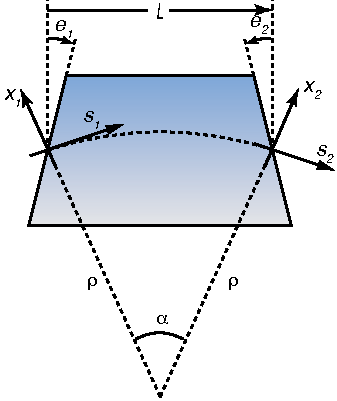
\includegraphics{rbend-coords.pdf}}
  \hspace{1cm}
  \subfigure[sbend]
  {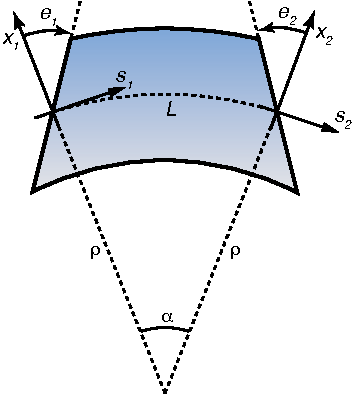
\includegraphics{sbend-coords.pdf}}
  \caption[Coordinate systems for (a) \vn{rbend}\ and (b) \vn{sbend}\ elements.]
{Coordinate systems for (a) \vn{rbend} and (b) \vn{sbend} elements.
For the bends drawn as viewed from ``above'' (viewed from positive $y$),
\vn{g}, \vn{angle}, \vn{rho}, \vn{e1} and \vn{e2} are all positive.}
  \label{f:bend}
\end{figure}

  \begin{description}
  \index{l}\index{l_chord}\index{l_arc}
  \item[l, l_chord]  \Newline
For compatibility with MAD, for an \vn{rbend}, \vn{l} is the chord
length and not the arc length as it is for an \vn{sbend}.  However,
after reading in a lattice, \bmad will internally convert all
\vn{rbend}s into \vn{sbend}s, additionally, the \vn{l_chord} attribute
will be set to the input \vn{l}, and \vn{l} will be set to the true
path length (see above). Alternatively, instead of setting \vn{l}, the
\vn{l_arc} attribute can be set to the true arc length.
  \index{h1}\index{h2}
  \item[h1, h2] \Newline
The attributes \vn{h1} and \vn{h2} are the curvature of the entrance
and exit pole faces. They are present for compatibility with MAD but
are not yet implemented in terms of tracking and other calculations.
  \index{e1}\index{e2}
  \item[e1, e2] \Newline
The rotation angle of the entrance pole face is \vn{e1} and at the
exit face it is \vn{e2}. Zero \vn{e1} and \vn{e2} for an \vn{rbend}
gives a rectangular magnet  (\fig{f:bend}a). Zero \vn{e1} and \vn{e2}
for an \vn{sbend} gives a wedge shaped magnet (\fig{f:bend}b).
An \vn{sbend} with an \vn{e1} = \vn{e2} = \vn{angle}/2 is equivalent 
to an \vn{rbend} with \vn{e1} = \vn{e2} = 0 (see above).
This formula holds for both positive and negative angles.
  \index{angle}
  \item[angle] \Newline
The total design bend angle. A positive \vn{angle} represents a
bend towards negative $x$ values (see \fig{f:local.coords}).
  \index{k1}\index{b1_gradient}
  \item[k1, b1_gradient] \Newline
The normalized and unnormalized quadrupole strength.
  \index{k2}\index{b2_gradient}
  \item[k2, b2_gradient] \Newline
The normalized and unnormalized sextupole strength. 
  \index{g}\index{rho}\index{g_err}
  \item[g, g_err, rho] \Newline
The design bending radius which determines the reference coordinate
system is \vn{rho} (see \sref{s:ref}). \vn{g} = 1/\vn{rho} is
the curvature function and is proportional to the design dipole
magnetic field. The true field strength is given by
\vn{g}~+~\vn{g_err} so changing \vn{g_err} leaves the design orbit
unchanged but varies a particle's orbit.
  \index{fint}\index{fintx}\index{hgapx}\index{hgapx}
  \item[fint, fintx, \Newline hgap, hgapx] \Newline
The field integrals for the entrance and
exit pole faces are give by \vn{fint} and \vn{fintx} respectively
\Begineq
  F_{int} = \int_{pole} \! \! ds \, \frac{B_y(s) (B_{y0} - B_y(s))}
  {2 H_{gap} B_{y0}^2}
\Endeq
with a similar equation for \vn{fintx}. In the equation $B_{y0}$ is
the field in the interior of the dipole and $H_{gap}$ is the pole half
gap.  The parameters \vn{hgap} and \vn{hgapx} are the half gaps at the
entrance and exit faces. If \vn{fint} or \vn{fintx} is given without a
value then a value of 0.5 is used. If \vn{fint} or \vn{fintx} is not
present, the default value of 0 is used. Note: \mad does not have the
\vn{fintx} and \vn{hgapx} attributes. \mad just assumes that the
values are the same for the entrance and exit faces. For compatibility
with \mad, if \vn{fint} is given but \vn{fintx} is not, then
\vn{fintx} is set equal to \vn{fint}. Similarly, \vn{hgapx} will be
set to \vn{hgap} if \vn{hgapx} is not given.

\index{Enge function}
\vn{fint} and \vn{hgap} can be related to the Enge function which is sometimes
used to model the fringe field. The Enge function is of the form
\Begineq
  B_y(s) = \frac{B_{y0}}{1 + \exp[P(s)]}
\Endeq
where
\Begineq
  P(s) = C_0 + C_1 \, s + C_2 \, s^2 + C_3 \, s^3 + \, \ldots
\Endeq
The $C_0$ term simply shifts where the edge of the bend is. If all the $C_n$
are zero except for $C_0$ and $C_1$ then 
\Begineq
  C_1 = \frac{1}{2 \,H_{gap} \, F_{int}}
\Endeq
  \index{tilt}
  \item[tilt] \Newline
The roll angle about the longitudinal axis at the entrance face of the
bend is given by \vn{tilt}.  \vn{tilt} = 0 bends the reference
trajectory in the $-x$ direction.  If the \vn{tilt} attribute is given
without any value then the value $\pi/2$ will be used. This makes for
a \vn{downward} pointing vertical bend. See \fig{f:tilt.bend}.
  \end{description}

The attributes \vn{g}, \vn{angle}, and \vn{l} are mutually dependent. If any two are
specified for an element \bmad will calculate the appropriate value
for the third.  After reading in a lattice, \vn{angle} is considered a
dependent variable (\sref{s:depend}).

Since internally all \vn{rbend}s are converted to \vn{sbend}s, if one wants to
vary the \vn{g} attribute of a bend and still keep the bend rectangular, an
overlay (\sref{s:overlay}) can be constructed to maintain the proper face angles.
For example:
\begin{example}
  l_ch = 0.54
  g_in = 1.52
  l_coef = asin(l_ch * g_in / 2) / g_in
  my_bend: rbend, l = l_ch, g = g_in
  my_overlay: overlay = \{my_bend, my_bend[e1]:l_coef, my_bend[e2]:l_coef\}, g = g_in
\end{example}
Notice that \vn{l_coef} is just \vn{arc_length/2}.

The \vn{n_ref_pass} attribute are only used
when a bend is part of a \vn{multipass} line and is used to set the
reference geometry of the bend. See section~\sref{s:multipass} for
more details.

In the local coordinate system (\sref{s:ref}), looking from ``above''
(bend viewed from positive $y$), and with \vn{tilt} = 0, a positive
\vn{angle} represents a particle rotating clockwise. In this
case. \vn{g} will also be positive. For counterclockwise rotation,
both \vn{angle} and \vn{g} will be negative but the length \vn{l} is
always positive. Also, looking from above, a positive \vn{e1}
represents a clockwise rotation of the entrance face and a positive
\vn{e2} represents a counterclockwise rotation of the exit face. This
is true irregardless of the sign of \vn{angle} and \vn{g}. Also it is
always the case that the pole faces will be parallel when
\begin{example}
  e1 + e2 = angle
\end{example}

\begin{figure}[tb]
  \centering
  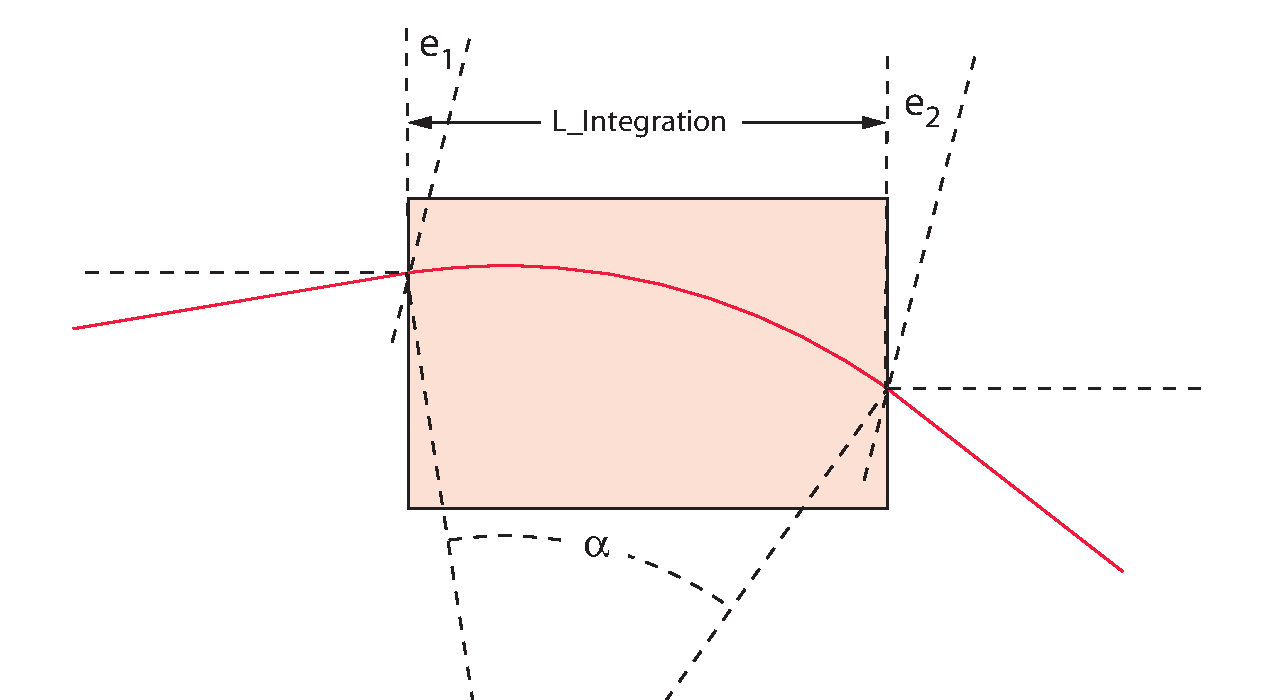
\includegraphics[width=5in]{true-rbend.pdf}
  \caption[True Rbend coordinates]{Coordinate system when \vn{ptc_field_geometry}
is set to \vn{true_rbend}.}
  \label{f:true.rbend}
\end{figure}

Example bend specification:
\begin{example}
  b03w: sbend, l = 0.6, k1 = 0.003, fint  ! gives fint = fintx = 0.5
\end{example}


\vn{ptc_field_geometry} determines how PTC integrates through a bend
if PTC is being used for tracking. Possible values for
\vn{ptc_field_geometry} are:
\begin{example}
  sector      ! Default
  straight
  true_rbend  ! Only valid for rbend elements
\end{example}
For \vn{sector} tracking, the tracking coordinate reference frame is
with respect to the arc of the reference trajectory. For \vn{straight}
tracking the tracking coordinate reference frame is with respect to the
chord line. For a bend where the number of integration steps is large
enough, and where there are no other fields besides the basic dipole
field, the results are the same.  When there are quadrupole or higher
order fields, the fields are expanded about the tracking reference
frame. Since Maxwell's equations must be satisfied, the higher order
fields will differ when tracking with \vn{sector} vs \vn{straight} the
difference in the fields will scale with the inverse of the bending
radius \vn{1/rho}. The above discussion is true for
\vn{ptc_exact_model} set to True, for \vn{ptc_exact_model} set to
False, a simplified sector tracking model is used in all cases.

The \vn{true_rbend} tracking of \vn{ptc_field_geometry} is used only
with \vn{rbend} elements and the entrance and exit faces must be parallel
as shown in \fig{f:true.rbend}. That is
\begin{example}
  e1 + e2 = 0
\end{example}
In this case, the tracking geometry is parallel, to the bend face as
shown in the figure. This can be an advantage in some situations but
Etienne discourages use of \vn{true_rbend} due to complications of how
to handle the reference frames in particular when you have more than
one of them in a row.

%-----------------------------------------------------------------
\section{Branch and Photon_Branch}
\label{s:branch}
\index{branch|hyperbf}
\index{photon_branch|hyperbf}

A \vn{branch} or \vn{photon_branch} element marks the start of an
alternative line for the beam. The only difference between \vn{branch}
and \vn{photon_branch} is that the default particle type for a
\vn{branch} is the same particle type in use at where the branching
occurs. The default particle type for a \vn{photon_branch} element is
a photon. See \sref{s:branching} for more details.

General \vn{branch} and \vn{photon_branch} attributes are:
\begin{center}
\tt
\begin{tabular}{|l|l||l|l|} \hline
  {\sl Attribute Class}  & \s              & {\sl Attribute Class}      & \s              \HH
  Description strings    & \ref{s:alias}   & Offsets                    & \ref{s:offset}  \HH
  Reference energy       & \ref{s:energy}  & Tracking \& transfer map   & \ref{c:methods} \HH
  Aperture Limits        & \ref{s:limit}   & Length                     & \ref{s:l}       \HH
                         &                 & Is_on                      & \ref{s:is.on}   \HH 
\end{tabular}
\end{center}
\toffset

Attributes specific to a \vn{branch} and \vn{photon_branch} elements are:
\begin{example}
  direction    = <+/- 1>      ! Direction of branch.
  to_line      = <LineName>   ! What line to branch to.
  to_element   = <ElementID>  ! What element to in the line to attach to.
  new_branch   = <T/F>        ! Make a new branch from the to_line? Default = True.
\end{example}

Branch lines can themselves have branching elements. A branch line
always starts out tangential to the line it is branching from. The
\vn{direction} attribute of the branch element indicates whether the
branch line is outgoing in the forward direction (\vn{direction} = +1)
or incoming (\vn{direction} = -1). A \vn{patch} element
(\sref{s:patch}) can be used at the beginning of a branch line to
reorient the reference orbit as needed.  For \vn{direction} = -1, the
local coordinate system orientation is ``reversed''
using the transformation (cf.~\fig{f:global.coords})
\begin{equation}
  \theta \longrightarrow \theta + \pi \comma\qquad
  \phi   \longrightarrow -\phi \comma\qquad
  \psi   \longrightarrow -\psi 
\end{equation}
and the particle phase space coordinates are transformed using
\Begineq
  (x, p_x, y, p_y, z, p_z) \longrightarrow (-x, p_x, y, -p_y, -z, p_z)
\Endeq

If the branch line is to transport particles different from the
originating line the particle type and the beginning reference energy
must be set for that line using line parameter statements
(\sref{s:beginning}). This is useful, for example, for a photon branch
that is branching from a storage ring where the photon energy is not
simply related to the particle energy. 

Example showing an injection line branching to a ring branching to two
x-ray lines:
\begin{example}
  inj: line = (..., ring, ...)               ! Define the injection line
  use, inj                                   ! Injection line is the root
  ring_br: branch, to_line = ring, 
          geometry = closed                  ! Branch to the ring
  ring: line = (..., x_br, ..., x_br, ...)   ! Define the ring
  x_br: photon_branch, to_line = x_line 
  x_line: line = (...)                       ! Define the x-ray line
  x_line[E_tot] = 1e3
\end{example}

The \vn{new_branch} attribute is, by default, \vn{True} which means
that the lattice branch created out of the \vn{to_line} line is distinct
from other lattice branches of the same name. Thus, in the above example,
the two lattice branches made from the \vn{x_line}
will be distinct. If \vn{new_branch} is set to \vn{False}, a new lattice
branch will not be created if a lattice branch createda from the same
line already exists. This is useful, for example, when a chicane line
branches off from the main line and then branches back to it.

%-----------------------------------------------------------------
\section{Capillary}
\label{s:capillary}
\index{capillary|hyperbf}

A \vn{capillary} element is a glass tube that is used to focus x-ray
beams.

General \vn{capillary} attributes are:
\begin{center}
\tt
\begin{tabular}{|l|l||l|l|} \hline
  {\sl Attribute Class}  & \s              & {\sl Attribute Class}      & \s              \HH
  Description strings    & \ref{s:alias}  & Offsets                    & \ref{s:offset}  \HH
  Reference energy       & \ref{s:energy}  & Tracking \& transfer map   & \ref{c:methods} \HH
  Aperture Limits        & \ref{s:limit}   & Is_on                      & \ref{s:is.on}   \HH 
  Capillary Wall         & \ref{s:wall}    &                            &                 \HH
\end{tabular}
\end{center}
\toffset

\index{critical_angle_factor|hyperbf}
Attributes specific to a \vn{capillary} element are:
\begin{example}
  critical_angle_factor = <Real>    ! Critical angle * Energy (rad * eV)
\end{example}
The critical angle above which photons striking the capillary surface are
refracted into the capillary material scales as 1/Energy. The
constant of critical angle * energy is given by the \vn{critical_angle_factor}.

The inside wall of a capillary is defined using the same syntax used
to define the chamber wall for other elements (\sref{s:wall}).

%-----------------------------------------------------------------
\section{Collimators: Ecollimator and Rcollimator} 
\label{s:col}
\index{ecollimator|hyperbf}
\index{rcollimator|hyperbf}

An \vn{ecollimator} is a drift with elliptic collimation. An
\vn{rcollimator} is a drift with rectangular collimation.

General \vn{ecollimator} and \vn{rcollimator} attributes are:
\begin{center}
\tt
\begin{tabular}{|l|l||l|l|} \hline
  {\sl Attribute Class}  & \s              & {\sl Attribute Class}      & \s              \HH
  Description strings    & \ref{s:alias}   & Offsets                    & \ref{s:offset}  \HH
  Reference energy       & \ref{s:energy}  & Tracking \& transfer map   & \ref{c:methods} \HH
  Aperture Limits        & \ref{s:limit}   & Length                     & \ref{s:l}       \HH
  Symplectify            & \ref{s:symp}    & Integration settings       & \ref{s:integ}   \HH
  Hkick \& Vkick         & \ref{s:kick}    & Chamber wall               & \ref{s:wall}    \HH
\end{tabular}
\end{center}
\toffset

Note: Collimators are the exception to the rule that the aperture is
independent of any \vn{tilt}s. See \sref{s:limit} for more
details. Example:
\begin{example}
  d21: ecollimator, l = 4.5, x_limit = 0.09/2, y_limit = 0.05/2
\end{example}

%-----------------------------------------------------------------
\section{Crystal}
\label{s:crystal}
\index{crystal|hyperbf}

\begin{figure}[tb]
  \centering
  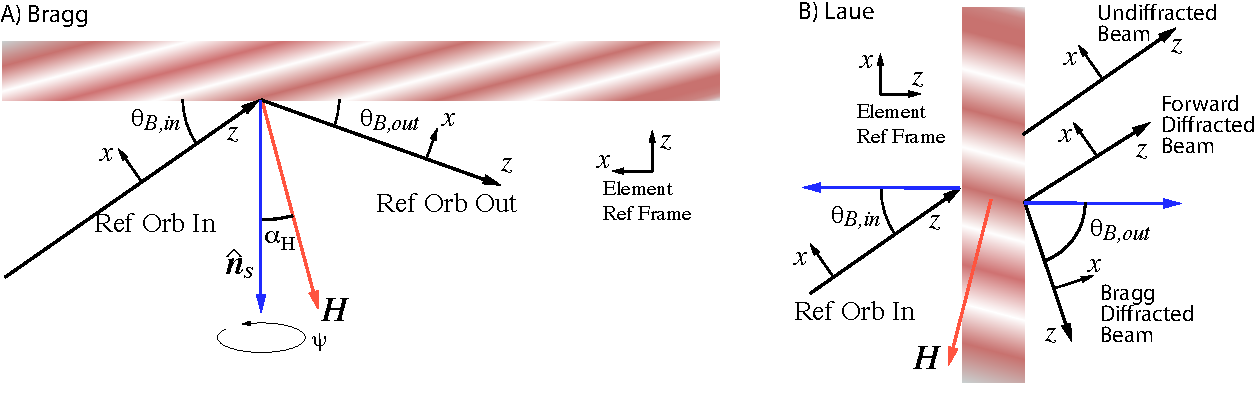
\includegraphics[width=5in]{crystal-ele.pdf}
  \caption[Crystal element geometry.]
{Crystal element geometry for Bragg reflections. 
The geometry shown is appropriate for zero
\vn{tilt} (reference trajectory in the $x$-$z$ plane). The angle
$\alpha_H$ (\vn{alpha_angle}) is the angle of the $\bfH$ vector with
respect to the surface normal $\bfhat n$. For $\psi$ (\vn{psi_angle})
zero, the incoming reference orbit, the outgoing reference orbit,
$\bfhat n$, and $\bfH$ are all coplanar. The element reference coordinates
where $\bfhat x$ is parallel to the surface normal establishes the coordinates
for specifying a rotation of $\bfH$ around the surface normal and specifying
a curvature of the surface.}
  \label{f:crystal}
\end{figure}

A \vn{crystal} element represents a crystal used for photon diffraction.

General \vn{crystal} attributes are:
\begin{center}
\tt
\begin{tabular}{|l|l||l|l|} \hline
  {\sl Attribute Class}  & \s              & {\sl Attribute Class}      & \s              \HH
  Description strings    & \ref{s:alias}  & Offsets                    & \ref{s:offset}  \HH
  Reference energy       & \ref{s:energy}  & Tracking \& transfer map   & \ref{c:methods} \HH
  Aperture Limits        & \ref{s:limit}   & Symplectify                & \ref{s:symp}    \HH
  Chamber Wall           & \ref{s:wall}    & Surface Curvature          & \ref{s:s.curve} \HH
\end{tabular}
\end{center}
\toffset

\index{graze_angle_err}\index{psi_angle}
\index{b_param}\index{bragg_angle}\index{crystal_type}
\index{tilt_err}\index{g_graze}
\index{follow_diffracted_beam}\index{thickness}
Attributes specific to a \vn{crystal} element are:
\begin{example}
  b_param                = <Real>    ! b parameter
  crystal_type           = <String>  ! Crystal material and reflection plane.
  graze_angle_err        = <Real>    ! Error in the graze angle.
  psi_angle              = <Real>    ! Rotation of H-vector about the surface normal.
  tilt_err               = <Real>    ! Error in the tilt angle.
  thickness              = <Real>    ! Thickness of crystal for Laue diffraction.
  follow_diffracted_beam = <Logic>   ! Track the diffracted or undiffracted beam?
  negative_graze_angle  = <Logic>    ! Use negative graze angle? Default is False.
\end{example}

\index{graze_angle_in}\index{graze_angle_out}\index{alpha_angle}
\index{tilt_corr}\index{d_spacing}\index{v_unitcell}\index{f0_re}
\index{f0_im}\index{fh_re}\index{fh_im}\index{ref_wave_length}
\index{c2_curve_tot}\index{c3_curve_tot}\index{c4_curve_tot}
Dependent variables (\sref{s:depend}) specific to a \vn{crystal} element are:
\begin{example}
  alpha_angle      ! Angle of H-vector with respect to the surface normal.
  bragg_angle      ! Nominal Bragg angle at the reference wave length. 
  d_spacing        ! Lattice plane spacing. 
  f0_re            ! Real part of f0
  f0_im            ! Imaginary part of f0
  fh_re            ! Real part of fh
  fh_im            ! Imaginary part of fh
  graze_angle_in   ! Angle between incoming beam and mirror surface.
  graze_angle_out  ! Angle between incoming beam and mirror surface.
  ref_wavelength   ! Reference wavelength
  ref_cap_gamma    ! \(\Gamma\) at the reference wavelength.
  tilt_corr        ! Tilt correction due to a finite psi_angle.
  v_unitcell       ! Unit cell volume. 
\end{example}

The \vn{crystal_type} attribute defines the crystal material and
diffraction lattice plane. The syntax is \vn{"ZZZ(ijk)"} where \vn{ZZZ}
is the atomic formula for the material and \vn{ijk} are the Miller
indices for the diffraction plane. For example, \vn{"Si(111)"}. The
atomic formula is case sensitive so, for example, \vn{SI} is not
acceptable.  Given the \vn{crystal_type} along with the reference
photon energy (\sref{s:energy}), the spacing between lattice planes
(\vn{d_spacing}), the unit cell volume (\vn{v_unitcell}), and the
structure factor\cite{b:batterman} values \vn{f0_re}, \vn{f0_im},
\vn{fh_re}, \vn{fh_im} can be computed.

The \vn{b_param} is the standard asymmetry factor
\Begineq
  b = \frac{\sin(\alpha_H + \theta_B)}{\sin(\alpha_H - \theta_B)} 
\Endeq
where $\theta_B$ is the Bragg angle (\vn{bragg_angle}) 
\Begineq
  \theta_B = \frac{\lambda}{d \, \sin\theta}
\Endeq
and $\alpha_H$ (\vn{alpha_angle}) is the angle of the reciprocal
lattice $\bfH$ vector with respect to the surface normal as shown in
\fig{f:crystal}.  If \vn{b_param} is set to -1 then there is
Bragg reflection and \vn{alpha_H} is zero. If \vn{b_param} is set to 1
then there is Laue diffraction again with \vn{alpha_H} zero. With the
orientation shown in \fig{f:crystal}, \vn{alpha_H} is positive.

The \vn{thickness} parameter is used with Laue diffraction only.

The \vn{follow_diffracted_beam} parameter sets whether the diffracted
beam or the undiffracted beam tracked. This parameter is only relevant
with Laue diffraction.

If \vn{psi_angle} is zero, the incoming reference orbit, the outgoing
reference orbit, $\bfhat n$ and $\bfH$ are all coplanar. A non-zero
\vn{psi_angle} Rotates the $\bfH$ vector around the $+\bfhat x$ axis
of the \vn{Element Reference Frame} (See \fig{f:crystal}).

The reference trajectory for a \vn{crystal} is that of a zero length
bend (\sref{s:mirror.coords}) and hence the length (\vn{l}) parameter
of a crystal is fixed at zero. The orientation of the reference
trajectory with respect to the crystal surface is specified by the
incoming graze angle \vn{graze_angle_in} ($\theta_{g,in}$) and
outgoing graze angle \vn{graze_angle_out} ($\theta_{g,out}$) as shown
in \fig{f:crystal}. These angles are computed from the photon
reference energy and the other crystal parameters such that a photon
with the reference energy traveling along the reference trajectory
will be in the center of the Darwin curve (\sref{s:crystal.tracking}).
If \vn{negative_graze_angle} is set to \vn{True}, 
\vn{graze_angle_in} and \vn{graze_angle_out} will be negative. This is
equivalent to setting \vn{tilt} to \vn{pi}.

The reference trajectory in the global coordinate system
(\sref{s:global}) is determined by the value of the \vn{tilt}
parameter along with the value of \vn{graze_angle_in} +
\vn{graze_angle_out}. A positive \vn{graze_angle_in} +
\vn{graze_angle_out} bends the reference trajectory in the same
direction as a positive \vn{g} for a bend element. The
\vn{graze_angle_err} and \vn{tilt_err} parameters affect the
orientation of the \vn{crystal} in the global reference system but do
not affect the reference trajectory.

A \vn{crystal} may be offset and pitched (\ref{s:offset}). The incoming
local reference coordinates are used for these misalignments. The
\vn{x_pitch} and \vn{y_pitch} parameters can be related to the
\vn{graze_angle_err} and \vn{tilt_err} parameters. For example, with
zero \vn{tilt}, a positive \vn{x_pitch} is equivalent to a negative
\vn{graze_angle_err} of the same magnitude, and a positive
\vn{y_pitch} is equivalent to a negative \vn{tilt_err} of the same
magnitude.

When a crystal is bent (\sref{s:s.curve}), the $\bfH$ vector is
assumed follow the surface curvature. That is, it is assumed that the
lattice planes are curved by the bending.

Example:
\begin{example}
  crystal_ele: crystal, crystal_type = 'Si(111)', b_param = -1
\end{example}

%-----------------------------------------------------------------
\section{Custom}
\label{s:custom}
\index{custom|hyperbf}

A \vn{custom} element is an element whose properties are defined
outside of the standard \bmad subroutine library. That is, to use a
custom element, some programmer must write the appropriate custom
routines which are then linked with the \bmad subroutines into a
program. \bmad will call the custom routines at the appropriate time
to do tracking, transfer matrix calculations, etc. See the programmer
who wrote the custom routines for more details! See
\sref{s:custom.ele} on how to write custom routines.

\index{tracking_method}\index{mat6_calc_method}\index{field_calc}
As an alternative to defining a custom element, standard elements can
be ``customized'' by setting one or more of the following attributes
to \vn{custom}:
\begin{example}
  tracking_method       \sref{s:tkm}
  mat6_calc_method      \sref{s:xfer}
  field_calc            \sref{s:integ}
  aperture_type         \sref{s:limit}
\end{example}
As with a custom element, setting one of these attributes to
\vn{custom} necessitates the use of custom code to implement the
corresponding calculation.

General \vn{custom} attributes are:
\begin{center}
\tt
\begin{tabular}{|l|l||l|l|} \hline
  {\sl Attribute Class}  & \s                & {\sl Attribute Class}      & \s              \HH
  Aperture Limits        & \ref{s:limit}     & Is_on                      & \ref{s:is.on}   \HH
  Chamber wall           & \ref{s:wall}      & Length                     & \ref{s:l}       \HH
  Description strings    & \ref{s:alias}     & Offsets, pitches, and tilt & \ref{s:offset}  \HH
  Field table or map     & \ref{s:em.fields} & Reference energy           & \ref{s:energy}  \HH 
  Fringe fields          & \ref{s:fringe}    & Symplectify                & \ref{s:symp}    \HH
  Integration settings   & \ref{s:integ}     & Tracking \& transfer map   & \ref{c:methods} \HH
\end{tabular}
\end{center}
\toffset

\index{delta_e}
\index{val1,  ..., Val12}
Attributes specific to a \vn{custom} element are
\begin{example}
  val1, ..., val12 = <Real>  ! Custom values 
  delta_e          = <Real>  ! Change in energy.
\end{example}

\vn{delta_e} is the energy gain of the {\it reference} particle
between the starting edge of the element and the ending edge.

Example:
\begin{example}
  c1: custom, l = 3, val4 = 5.6, val12 = 0.9, descrip = 'params.dat'
\end{example}
In this example the \vn{descrip} string is being used to specify a
file that contains parameters for the element.

%-----------------------------------------------------------------
\section{Drift}
\label{s:drift}
\index{drift|hyperbf}

A \vn{drift} element is a space free and clear of any fields.

General \vn{drift} attributes are:
\begin{center}
\tt
\begin{tabular}{|l|l||l|l|} \hline
  {\sl Attribute Class}  & \s              & {\sl Attribute Class}      & \s              \HH
  Aperture Limits        & \ref{s:limit}   & Offsets, pitches, and tilt & \ref{s:offset}  \HH
  Chamber wall           & \ref{s:wall}    & Reference energy           & \ref{s:energy}  \HH 
  Description strings    & \ref{s:alias}   & Symplectify                & \ref{s:symp}    \HH 
  Integration settings   & \ref{s:integ}   & Tracking \& transfer map   & \ref{c:methods} \HH
  Length                 & \ref{s:l}       &                            &                 \HH
\end{tabular}
\end{center}
\toffset

Example:
\begin{example}
  d21: drift, l = 4.5
\end{example}

%-----------------------------------------------------------------
\section{E_Gun}
\label{s:e.gun}
\index{e_gun|hyperbf}

An \vn{e_gun} element is an electron gun.
General \vn{e_gun} attributes are:
\begin{center}
\tt
\begin{tabular}{|l|l||l|l|} \hline
  {\sl Attribute Class}  & \s              & {\sl Attribute Class}      & \s              \HH
  Symplectify            & \ref{s:symp}    & Offsets, pitches, and tilt & \ref{s:offset}  \HH
  Description strings    & \ref{s:alias}  & Is_on                      & \ref{s:is.on}   \HH 
  Reference energy       & \ref{s:energy}  & Tracking \& transfer map   & \ref{c:methods} \HH
  Aperture Limits        & \ref{s:limit}   & Length                     & \ref{s:l}       \HH
  Hkick \& Vkick         & \ref{s:kick}    & a$n$, b$n$ multipoles      & \ref{s:multip}  \HH
  Integration settings   & \ref{s:integ}   & Chamber wall               & \ref{s:wall}    \HH
\end{tabular}
\end{center}
\toffset

The attributes specific to an \vn{e_gun} are 
\index{voltage}\index{voltage_err}
\index{gradient}\index{gradient_err}
\begin{example}
  gradient     = <Real>    ! Gradient.
  gradient_err = <Real>    ! Gradient error.
  voltage      = <Real>    ! Voltage. Dependent attribute (\sref{s:depend}). 
  voltage_err  = <Real>    ! Voltage error. Dependent attribute (\sref{s:depend}). 
\end{example}
The \vn{voltage} is simply related to the \vn{gradient} via the element length \vn{l}:
\begin{example}
  voltage = gradient * l
\end{example}
If the \vn{voltage} is set to a non-zero value, the length \vn{l} must
also be non-zero to keep the gradient finite.

\index{marker}\index{null_ele}
The \vn{e_gun} element is meant to solve the problem of simulating
electrons as they are generated from a cathode. The fact that these
electrons can have zero initial momentum presents a special problem
(\sref{s:energy}). As a result, the use of \vn{e_gun} elements are
restricted and they can only be used in a ``linear''
(non-recirculating) lattice branch. Only one \vn{e_gun} can be present
in a lattice branch and, if it is present, it must be, except for
possibly \vn{marker} or \vn{null_ele} elements, the first element in
any branch.
 
Note: In order to be able to avoid problems with a zero reference
momentum at the beginning of the \vn{e_gun}, the reference momentum
and energy associated with an \vn{e_gun} element is calculated as
outlined in Section~\sref{s:energy}. Additionally, the reference
momentum at the exit end of the \vn{e_gun}, that is \vn{p0c}, must be
non-zero. Thus, for example, if \vn{p0c} is zero at the start of the
lattice, the \vn{e_gun} voltage must be non-zero. 

%-----------------------------------------------------------------
\section{Elseparator}
\label{s:elsep}
\index{elseparator|hyperbf}

An \vn{elseparator} is an electrostatic separator.

General \vn{elseparator} attributes are:
\begin{center}
\tt
\begin{tabular}{|l|l||l|l|} \hline
  {\sl Attribute Class}  & \s              & {\sl Attribute Class}      & \s              \HH
  a$n$, b$n$ multipoles      & \ref{s:multip}    & Integration settings       & \ref{s:integ}   \HH
  Aperture Limits            & \ref{s:limit}     & Is_on                      & \ref{s:is.on}   \HH
  Chamber wall               & \ref{s:wall}      & Length                     & \ref{s:l}       \HH
  Description strings        & \ref{s:alias}     & Offsets, pitches, and tilt & \ref{s:offset}  \HH
  Field table or map         & \ref{s:em.fields} & Reference energy           & \ref{s:energy}  \HH 
  Fringe Fields              & \ref{s:fringe}    & Symplectify                & \ref{s:symp}    \HH
  Hkick \& Vkick             & \ref{s:kick}      & Tracking \& transfer map   & \ref{c:methods} \HH
\end{tabular}
\end{center}
\toffset

\index{gap}
\index{e_field}
\index{voltage}
Attributes specific to an \vn{elseparator} element are:
\begin{example}
  gap = <Real> ! Distance between electrodes
  voltage      ! Voltage between electrodes. This is a dependent variable (\sref{s:depend}).
  e_field      ! Electric field. This is a dependent variable (\sref{s:depend}).
\end{example}

\index{hkick}
\index{vkick}
For an \vn{elseparator}, the kick is determined by \vn{hkick} and
\vn{vkick}. The \vn{gap} for an \vn{Elseparator} is used to compute
the electric field for a given kick. The voltage is a dependent
attribute determined by:
\begin{example}
  e_field (V/m) = sqrt(hkick^2 + vkick^2) * E_TOT / L
  voltage (V) = e_field * gap  
\end{example}

Example:
\begin{example}
  h_sep: elsep, l = 4.5, hkick = 0.003, gap = 0.11
\end{example}

%-----------------------------------------------------------------
\section{EM_Field}
\label{s:em.field}
\index{em_field|hyperbf}

An \vn{em_field} element can contain general electro-magnetic (EM)
fields. Both AC and DC fields are accommodated.  General \vn{em_field}
attributes are:
\begin{center}
\tt
\begin{tabular}{|l|l||l|l|} \hline
  {\sl Attribute Class}  & \s              & {\sl Attribute Class}      & \s              \HH
  Symplectify            & \ref{s:symp}    & Offsets, pitches, and tilt & \ref{s:offset}  \HH
  Description strings    & \ref{s:alias}   & Is_on                      & \ref{s:is.on}   \HH 
  Reference energy       & \ref{s:energy}  & Tracking \& transfer map   & \ref{c:methods} \HH
  Aperture Limits        & \ref{s:limit}   & Length                     & \ref{s:l}       \HH
  Hkick \& Vkick         & \ref{s:kick}    & a$n$, b$n$ multipoles      & \ref{s:multip}  \HH
  Integration settings   & \ref{s:integ}   & Chamber wall               & \ref{s:wall}    \HH
\end{tabular}
\end{center}
\toffset

\vn{em_field} elements will be created when elements are superimposed (\sref{s:super}) and there is
no other suitable element class.

%-----------------------------------------------------------------
\section{Fiducial}
\label{s:fiducial}
\index{fiducial|hyperbf}

A \vn{fiducial} element is used to orient the reference orbit of an entire lattice branch.

General \vn{floor_shift} element attributes are:
\begin{center}
\tt
\begin{tabular}{|l|l||l|l|} \hline
  {\sl Attribute Class}  & \s              & {\sl Attribute Class}      & \s              \HH
  Aperture Limits        & \ref{s:limit}   & Reference energy           & \ref{s:energy}  \HH
  Description strings    & \ref{s:alias}   & Tracking \& transfer map   & \ref{c:methods} \HH
  Is_on                  & \ref{s:is.on}   &                            &                 \HH
\end{tabular}
\end{center}
\toffset

\index{l}\index{x_offset}\index{y_offset}\index{z_offset}\index{tilt}
\index{x_pitch}\index{y_pitch}\index{origin_ele}
\index{x_origin}\index{y_origin}
\index{z_origin}\index{theta_origin}
\index{phi_origin}\index{psi_origin}
Attributes specific to a \vn{floor_shift} elements are:
\begin{example}
  x_origin        = <Real>    ! Absolute Reference x-position
  y_origin        = <Real>    ! Absolute Reference y-position
  z_origin        = <Real>    ! Absolute Reference z-position
  theta_origin    = <Real>    ! Absolute Refernce orientation angle.
  phi_origin      = <Real>    ! Absolute Refernce orientation angle.
  psi_origin      = <Real>    ! Absolute Refernce orientation angle.
  origin_ele      = <Name>    ! Reference element.
  x_offset        = <Real>    ! x offset from reference
  y_offset        = <Real>    ! y offset from reference
  z_offset        = <Real>    ! z offset from reference
  x_pitch         = <Real>    ! rotation in the reference coords.
  y_pitch         = <Real>    ! rotation in the reference coords.
  tilt            = <Real>    ! rotation in the reference coords.
\end{example}

For tracking purposes, the \vn{fiducial} element is considered to be a
zero length marker. That is, the transfer map through a \vn{fiducial}
element is the unit map.

A \vn{fiducial} element sets the reference orbit of itself and of the
elements around it. This can be thought of as a two step process. The
first step is to determine the global coordinates of the \vn{fiducial}
element itself and the second step is to shift the coordinates of the
elements around it.

\index{marker}\index{init_ele}
The floor coordinates of the \vn{fiducial} element are determined
starting with an \vn{origin reference point}. This reference point can
either be specified by specifying an absolute global position using
the attributes \vn{x_origin}, \vn{y_origin}, etc. or by specifying an
\vn{origin_ele} element. If specified, the \vn{origin_ele} element
must be a \vn{marker} or \vn{init_ele} element. If the \vn{origin_ele}
is specified, the alsolute reference position attributes
\vn{x_origin}, etc., are ignored.

Once the origin reference position is determined, the reference
position of the \vn{fiducial} element is calculated using the offset
attributes \vn{x_offset}, \vn{x_pitch} as outlined in \sref{s:patch.coords}.

\index{flexible patch}\index{patch}
Once the position of the \vn{fiducial} element is calculated, all
elements of the lattice branch the \vn{fiducial} element is contained
in, {\em both} the upsteam and downstream elements, are shifted so
that everything is consistant. That is, the \vn{fiducial} element
orients the entire lattice branch. The exception here is that if there
are \vn{flexible} \vn{patch} elements (\sref{s:patch}) in the lattice
branch, the \vn{fiducial} element will only determine the positions up
to the \vn{flexible} \vn{patch} element. 

Example: A lattice branch with elements 0 through 103 has a
\vn{fiducial} element at position 34 and a \vn{flexible} \vn{patch} at
postion 67. In this case the \vn{fiducial} element will determine the
reference orbit for elements 0 through 66.

Rules: 
  \begin{description}
  \item
If a \vn{origin_ele} is specified, the position of this element must
to calculatd before the the position of the \vn{fiducial} element is
calculated (\sref{s:ref}). This means, the \vn{origin_ele} must be in
a prior lattice branch from the branch the \vn{fiducial} element is in
or the \vn{origin_ele} in the same branch as the \vn{fiducial} element
but is positioned upstream from the \vn{fiducial} element and there is
a \vn{flexible} \vn{patch} in between the two elements.
  \item
If a \vn{fiducial} element affets the position of element 0 in the
lattice branch (that is, there are no flexible \vn{branch} elements
inbetween), any positioning of element 0 via \vn{beginning} or
\vn{line parameter} statements (\sref{s:beginning}) are ignored.
  \item
\vn{Fiducial} elements must not over constrain the lattice geometry.
For example, two \vn{fiducial} elements may not appear in the same
lattice branch unless separated by a \vn{flexible} \vn{patch}. 

Another example is that if there are no flexible \vn{patch} elements
in the lattice, and if branch \vn{A} has a \vn{branch} element
connecting to branch \vn{B}, the geometry of branch \vn{A} will be
calculated first and the geometry of branch \vn{B} can then be
calculated from the known coordinates of the \vn{branch} element. If
branch \vn{B} contains a \vn{fiducial} element then this is an error
since the coordinate calculation never backtracks to recalculate the
coordinates of the elements of a branch once the calculation has
finished with that branch.
  \end{description}

Example:
\begin{example}
  f1: fiducial, origin_ele = mark1, x_offset = 0.04
\end{example}

%-----------------------------------------------------------------
\section{Floor_Shift}
\label{s:floor.ele}
\index{floor_shift|hyperbf}

A \vn{floor_shift} element shifts the reference orbit in the global
coordinate system without affecting particle tracking. Also see
\vn{patch} (\sref{s:patch}) and \vn{fiducial} (\sref{s:fiducial})
elements.

General \vn{floor_shift} element attributes are:
\begin{center}
\tt
\begin{tabular}{|l|l||l|l|} \hline
  {\sl Attribute Class}  & \s              & {\sl Attribute Class}      & \s              \HH
  Aperture Limits        & \ref{s:limit}   & Length                     & \ref{s:l}       \HH
  Description strings    & \ref{s:alias}   & Reference energy           & \ref{s:energy}  \HH
  is_on                  & \ref{s:is.on}   & Tracking \& transfer map   & \ref{c:methods} \HH
\end{tabular}
\end{center}
\toffset

\index{l}\index{x_offset}\index{y_offset}
\index{z_offset}\index{tilt}
\index{x_pitch}\index{y_pitch}
Attributes specific to a \vn{floor_shift} elements are:
\begin{example}
  l               = <Real>    ! Length
  x_offset        = <Real>    ! x offset from previous element
  y_offset        = <Real>    ! y offset from previous element
  z_offset        = <Real>    ! z offset from previous element
  x_pitch         = <Real>    ! rotation in the reference coords.
  y_pitch         = <Real>    ! rotation in the reference coords.
  tilt            = <Real>    ! rotation in the reference coords.
\end{example}

The \vn{floor_shift} element shifts the reference orbit relative to the
proceeding element. Unlike the \vn{patch element} \sref{s:patch}, the
transfer map through a \vn{floor_shift} element will be the unit
map. That is, the phase space coordinates of a particle will not
change when tracking through a \vn{floor_shift} element. The reference
position transformation through a \vn{floor_shift} element is given in
Section~\sref{s:patch.coords}.

The \vn{l} attribute can be used to adjust the longitudinal $s$
position.

The \vn{floor_shift} element can be used, for
example, to restore the correct geometry when a section of the lattice
is represented by, say, a \vn{taylor} type element.

PTC does not have an analogous element for the \vn{Floor_shift}
element. When converting to PTC, a \vn{floor_shift} element will be treated
as a \vn{marker} element.

Example: 
\begin{example}
  floor: floor_shift, z_offset = 3.2
\end{example}
This is equivalent to a drift.

%-----------------------------------------------------------------
\section{Girder}
\label{s:girder}
\index{girder|hyperbf}

A \vn{girder} is a support structure that orients the elements that
are attached to it in space.

General \vn{girder} attributes are:
\begin{center}
\tt
\begin{tabular}{|l|l||l|l|} \hline
  {\sl Attribute Class}  & \s              & {\sl Attribute Class}      & \s              \HH
  Description strings    & \ref{s:alias}  & Offsets, pitches, and tilt & \ref{s:offset}  \HH 
\end{tabular}
\end{center}
\toffset

Attributes specific to a \vn{girder} are:
\begin{example}
  girder = \{<List>\}   ! List of elements on the Girder
  s_center              ! Center of the girder
\end{example}

\index{x_offset}\index{y_pitch}\index{tilt}\index{s_center}
When a \vn{girder} overlays an element, then that elements
orientation attributes (\vn{x_offset}, \vn{y_pitch}, \vn{tilt}, etc.) 
give the orientation of
the element with respect to the \vn{girder}. An example will make this clear:
\begin{example}
  q1: quad, l = 2
  q2: quad, l = 4, x_offset = 0.2, x_pitch = 0.01
  d: drift, l = 8
  ib: girder = \{q1, q2\}, x_pitch = 0.1, x_offset = 0.3
  this_line: line = (q1, d, q2)
  use, this_line
\end{example}
\index{overlay}
In this example \vn{ib} supports elements \vn{q1} and \vn{q2}. The
\vn{s_center} of \vn{ib} is at $s = 7$~meters (\vn{ib} starts at $s =
0$ which is the beginning of \vn{q1} and ends at $s = 14$ which is the
end of \vn{q2}). Like other elements, pitch is calculated from the
center of a \vn{girder} element (see Sec.~\ref{s:offset}). The center
of \vn{q2} is at $s = 12$ so the distance between the center of
\vn{ib} and \vn{q2} is $ds = 5$. The pitch of \vn{ib} produces an
offset at the center of \vn{q2} of $0.5 = 0.1 * 5$. This, added to the
offsets of \vn{ib} and \vn{q2}, give the total offset of \vn{q2} to be
$1.0 = 0.5 + 0.3 + 0.2$. The total \vn{x_pitch} of \vn{q2} is $0.11 =
0.1 + 0.01$. From the above example it can be seen that a \vn{girder}
looks similar to an \vn{Overlay} (see Sec.~\ref{s:overlay}). It would,
however, take six \vn{Overlays} to simulate the effect of a single
\vn{girder}.

The \vn{girder} statement syntax is:
\begin{example}
  <element_name>: GIRDER = \{<ele1>, <ele2>, ..., <eleN> \}, ...
\end{example}
A \vn{girder} element will be created for each section of the lattice
where there is a ``consecutive'' sequence of ``slave'' elements
\vn{<ele1>} through \vn{<eleN>}.  This section of the lattice from
\vn{<ele1>} through \vn{<eleN>} is called the ``girder support
region''.  ``Consecutive'' here means there are no other elements in the
girder support region except for possibly \vn{drift} and/or \vn{marker}
elements.  \vn{Drift} elements cannot be controlled by a girder and
should not appear in the girder slave list. If a drift-like element is
desired, use a \vn{pipe} element instead. \vn{Marker} elements present
in a girder support region, but not mentioned in the girder slave
list, are simply ignored.

Wild card characters (\sref{s:lat.attribs}) can be used in any element
name in the girder slave list. Additionally, beam line names
(\sref{s:lines.wo.arg}) can be used. In this case, any \vn{drift} elements
within a beam line will be ignored.

%-----------------------------------------------------------------
\section{Hybrid}
\label{s:hybrid}
\index{hybrid|hyperbf}

A \vn{hybrid} element is an element that is formed by concatenating
other element together. \vn{hybrid} elements are not part of the input
lattice file but are created by a program, usually for speed purposes.

%-----------------------------------------------------------------
\section{Init_Ele}
\label{s:init.ele}
\index{init_ele|hyperbf}

An \vn{init_ele} element, named \vn{BEGINNING}, is placed at the
beginning of every branch (\sref{s:branching}) of a lattice to mark
the start of the branch. The \vn{init_ele} always has element index 0
(\sref{c:lat.concepts}).

\vn{init_ele} attributes are generally set using either \vn{parameter}
(\sref{s:param}) or \vn{beginning} (\sref{s:beginning}) statements.
In particular the initial energy may be set (\sref{s:energy}).

%-----------------------------------------------------------------
\section{Instrument, Monitor, and Pipe}
\label{s:monitor}
\index{instrument|hyperbf}
\index{monitor|hyperbf}
\index{pipe|hyperbf}

Essentially \bmad treats \vn{instrument}, \vn{monitor}, and \vn{pipe}
elements like a \vn{drift}. There is a difference, however, when
superimposing elements (\sref{s:super}). For example, a
\vn{quadrupole} superimposed on top of a \vn{drift} results in a free
\vn{quadrupole} element in the tracking part of the lattice and no
lord elements are created. On the other hand, a \vn{quadrupole}
superimposed on top of a \vn{monitor} results in a \vn{quadrupole}
element in the tracking part of the lattice and this \vn{quadrupole}
element will have two lords: A \vn{quadrupole} superposition lord and
a \vn{monitor} superposition lord.

General \vn{instrument}, \vn{monitor}, and \vn{pipe} attributes are:
\begin{center}
\tt
\begin{tabular}{|l|l||l|l|} \hline
  {\sl Attribute Class}  & \s                  & {\sl Attribute Class}      & \s              \HH
  Symplectify            & \ref{s:symp}        & Offsets, pitches, and tilt & \ref{s:offset}  \HH
  Reference energy       & \ref{s:energy}      & Tracking \& transfer map   & \ref{c:methods} \HH
  Aperture Limits        & \ref{s:limit}       & Length                     & \ref{s:l}       \HH
  Description strings    & \ref{s:alias}      & Is_on                      & \ref{s:is.on}   \HH 
  Integration settings   & \ref{s:integ}       & Hkick \& Vkick             & \ref{s:kick}    \HH
  Instrumental variables & \ref{s:meas.attrib} & Chamber wall               & \ref{s:wall}    \HH
\end{tabular}
\end{center}
\toffset

\index{x_offset}
\index{y_offset}
\index{x_pitch}
\index{y_pitch}
\index{tilt}
The \vn{offset}, \vn{pitch}, and \vn{tilt} attributes are not
used by any \bmad routines. If these attributes are used by a program
they are typically used to simulate such things as measurement
offsets. The \vn{is_on} attribute is also not used by \bmad
proper. Example:
\begin{example}
  d21: instrum, l = 4.5
\end{example}

%-----------------------------------------------------------------
\section{Kickers Horizontal and Vertical: Hkicker and Vkicker}
\label{s:hvkicker}
\index{hkicker|hyperbf}
\index{vkicker|hyperbf}

An \vn{hkicker} gives a beam a horizontal kick and a \vn{vkicker} gives a 
beam a vertical kick. Also see the \vn{kicker} (\sref{s:kicker}) element.

General \vn{hkicker} \vn{vkicker} attributes are:
\begin{center}
\tt
\begin{tabular}{|l|l||l|l|} \hline
  {\sl Attribute Class}  & \s              & {\sl Attribute Class}      & \s              \HH
  a$n$, b$n$ multipoles      & \ref{s:multip}    & Integration settings       & \ref{s:integ}   \HH
  Aperture Limits            & \ref{s:limit}     & Is_on                      & \ref{s:is.on}   \HH
  Chamber wall               & \ref{s:wall}      & Length                     & \ref{s:l}       \HH
  Description strings        & \ref{s:alias}     & Offsets, pitches, and tilt & \ref{s:offset}  \HH
  Field table or map         & \ref{s:em.fields} & Reference energy           & \ref{s:energy}  \HH 
  Fringe Fields              & \ref{s:fringe}    & Symplectify                & \ref{s:symp}    \HH
  Hkick \& Vkick             & \ref{s:kick}      & Tracking \& transfer map   & \ref{c:methods} \HH
\end{tabular}
\end{center}
\toffset

\index{kick}
\index{hkick}
\index{vkick}
Note that \vn{hkicker} and \vn{vkicker} elements use the
\vn{kick} attribute while a \vn{kicker} uses the \vn{hkick} and \vn{vkick} 
attributes. Example:
\begin{example}
  h_kick: hkicker, l = 4.5, kick = 0.003
\end{example}

%-----------------------------------------------------------------
\section{Kicker}
\label{s:kicker}
\index{kicker|hyperbf}

\index{hkick}
\index{vkick}
\index{h_displace}
\index{v_displace}
A \vn{kicker} can deflect a beam in both planes. Note that a
\vn{kicker} uses the \vn{hkick} and \vn{vkick} attributes while
\vn{hkicker} and \vn{vkicker} elements use the \vn{kick} attribute. 
In addition, a \vn{kicker} can apply a displacement to a particle
using the \vn{h_displace} and \vn{v_displace} attributes.

General \vn{kicker} attributes are:
\begin{center}
\tt
\begin{tabular}{|l|l||l|l|} \hline
  {\sl Attribute Class}      & \s              & {\sl Attribute Class}        & \s              \HH
  a$n$, b$n$ multipoles      & \ref{s:multip}    & Integration settings       & \ref{s:integ}   \HH
  Aperture Limits            & \ref{s:limit}     & Is_on                      & \ref{s:is.on}   \HH
  Chamber wall               & \ref{s:wall}      & Length                     & \ref{s:l}       \HH
  Description strings        & \ref{s:alias}     & Offsets, pitches, and tilt & \ref{s:offset}  \HH
  Field table or map         & \ref{s:em.fields} & Reference energy           & \ref{s:energy}  \HH 
  Fringe Fields              & \ref{s:fringe}    & Symplectify                & \ref{s:symp}    \HH
  Hkick \& Vkick             & \ref{s:kick}      & Tracking \& transfer map   & \ref{c:methods} \HH
\end{tabular}
\end{center}
\toffset

Example:
\begin{example}
  a_kick: kicker, l = 4.5, hkick = 0.003
\end{example}

%-----------------------------------------------------------------
\section{Lcavity}
\label{s:lcav}
\index{lcavity|hyperbf}

An \vn{lcavity} is a LINAC accelerating cavity.
The main difference between an \vn{rfcavity} and an
\vn{lcavity} is that, unlike an \vn{rfcavity}, the reference energy
(\sref{s:phase.space}) through an \vn{lcavity} is not constant.

General \vn{lcavity} attributes are:
\begin{center}
\tt
\begin{tabular}{|l|l||l|l|} \hline
  {\sl Attribute Class}      & \s                & {\sl Attribute Class}      & \s                 \HH
  Aperture Limits            & \ref{s:limit}     & Length                     & \ref{s:l}          \HH
  Chamber wall               & \ref{s:wall}      & Offsets, pitches, and tilt & \ref{s:offset}     \HH
  Description strings        & \ref{s:alias}     & Reference energy           & \ref{s:energy}     \HH 
  Field table or map         & \ref{s:em.fields} & RF Couplers                & \ref{s:rf.coupler} \HH
  Fringe Fields              & \ref{s:fringe}    & RF Wakes                   & \ref{s:rf.wakes}   \HH
  Hkick \& Vkick             & \ref{s:kick}      & Symplectify                & \ref{s:symp}       \HH
  Integration settings       & \ref{s:integ}     & Tracking \& transfer map   & \ref{c:methods}    \HH
  Is_on                      & \ref{s:is.on}     &                            &                    \HH
\end{tabular}
\end{center}
\toffset

The attributes specific to an \vn{lcavity} are 
\index{gradient}\index{phi0}\index{n_cell}
\index{dphi0}\index{e_loss}
\index{rf_frequency}\index{voltage}
\begin{example}
  gradient       = <Real>    ! Accelerating gradient (V/m).
  gradient_err   = <Real>    ! Accelerating gradient error (V/m).
  phi0           = <Real>    ! Phase (rad/2\(\pi\)) of the reference particle with 
                             !   respect to the RF. phi0 = 0 is on crest.
  dphi0          = <Real>    ! Phase with respect to a multipass lord (rad/2\(\pi\)).
  phi0_err       = <Real>    ! Phase error (rad/2\(\pi\))
  dphi0_ref      = <Real>    ! Phase offset used to deal with absolute time tracking
                             !  and other issues (see below).
  e_loss         = <Real>    ! Loss parameter for short range wake fields (V/Coul).
  rf_frequency   = <Real>    ! Rf frequency (Hz).
  voltage                    ! Cavity voltage. Dependent attribute (\sref{s:depend}).
  n_cell         = <Integer> ! Number of cavity cells. Default is 1.
\end{example}
The dependent variable \vn{voltage} attribute can be used in place of
\vn{gradient} as discussed in \sref{s:depend}.  \vn{voltage} is a
dependent attribute and is defined to be
\begin{example}
  voltage = gradient * L
\end{example}

The energy kick felt by a particle is 
\begin{example}
  dE = gradient_tot * L * cos(twopi * (phi_particle + phi_ref))
\end{example}
\index{multipass}
where the total gradient is
\begin{example}
  gradient_tot = gradient + gradient_err
\end{example}
the phase \vn{phi_ref} is
\begin{example}
  phi_ref = phi0 + dphi0 + phi0_err + dphi0_ref
\end{example}
and \vn{phi_particle} is
\begin{example}
  phi_particle = -z * rf_frequency / velocity  ! With relative time tracking (\sref{s:rf.time})
               =  t_particle * rf_frequency    ! With absolute time tracking
\end{example}
With \vn{relative time tracking}, the phase, \vn{phi_particle}, of the
particle with respect to the cavity's internal clock is proportional
to \vn{z} -- the particles' phase space coordinate
(\sref{s:phase.space}). With \vn{absolute time tracking},
\vn{phi_particle} is proportional to the absolute time the particle
reaches the cavity. See section~\sref{s:rf.time} for a discussion on
relative verses absolute time tracking. The
\vn{parameter[absolute_time_tracking]} switch (\sref{s:param}) sets
the type of tracking for a lattice.

\vn{dphi0} is only to be used to shift the phase with respect to a
\vn{multipass} lord. See \sref{s:multipass}.

\vn{dphi0_ref} is a phase calculated by \bmad's RF auto-phase module
(\sref{s:em.fields}).

The energy change of the reference particle is just the energy change for a 
particle with $z = 0$ and no phase or gradient errors. Thus
\begin{example}
  dE(reference) = gradient * L * cos(twopi * phi_ref)
\end{example}

The energy kick for a \bmad \vn{lcavity} is consistent with MAD. 
Note: The MAD8 documentation for an \vn{lcavity} has a wrong
sign. Essentially the MAD8 documentation gives
\begin{example}
  dE = gradient * L * cos(twopi * (phi_ref - phi(z))) ! WRONG
\end{example}
This is incorrect. 

When short-range wake fields are being simulated, with
\vn{bmad_com%sr_wakes_on = True} (\sref{s:bmad.params}), the
\vn{e_loss} attribute can be used to modify the gradient in order to
maintain a constant average energy gain. That is, \vn{e_loss} can be
used to simulate the effect of a feedback circuit that attempts to
maintain the average energy of the bunch after the element constant.
The energy kick is then
\begin{example}
  dE(with wake) = dE + e_loss * n_part * e_charge 
\end{example}
\vn{n_part} is set using the \vn{parameter} statement (\sref{s:param})
and represents the number of particles in a bunch. \vn{e_charge} is
the charge on an electron (Table~\ref{t:constants}). Notice that the
\vn{e_loss} term is independent of the sign of the charge of the particle.

The transverse trajectory through an \vn{lcavity} is modeled using
equations developed by Rosenzweig and Serafini\cite{b:rosenzweig}
modified to give the correct phase-space area at non
ultra-relativistic energies.  See Section \sref{s:lcav.phys} for more
details.  Note: The transfer matrix for an \vn{lcavity} with finite
\vn{gradient} is never symplectic. See \sref{s:phase.space}. In
addition, couplers (\sref{s:rf.coupler}) and HOM wakes
(\sref{s:rf.wakes}) can be modeled.

When using \vn{boris} or \vn{runge_kutta}, tracking (\sref{s:tkm})
through a field map (\sref{s:em.fields}), the \vn{bmad_standard} field
is \vn{n_cell} half wave resonators.

Example:
\begin{example}
  lwf: lcavity, l = 2.3, rf_frequency = 500e6, voltage = 20e6
\end{example}

%-----------------------------------------------------------------
\section{Marker}
\label{s:mark}
\index{marker|hyperbf}

A \vn{marker} is a zero length element meant to mark a position. 

General \vn{marker} attributes are:
\begin{center} 
\tt
\begin{tabular}{|l|l||l|l|} \hline
  {\sl Attribute Class}  & \s                  & {\sl Attribute Class}      & \s              \HH
  Description strings    & \ref{s:alias}      & Is_on                      & \ref{s:is.on}   \HH 
  Reference energy       & \ref{s:energy}      & Offsets and tilt           & \ref{s:offset}  \HH
  Aperture Limits        & \ref{s:limit}       & Tracking \& transfer map   & \ref{c:methods} \HH
  Instrumental variables & \ref{s:meas.attrib} &                            &                 \HH
\end{tabular}
\end{center}
\toffset

\index{x_ray_line_len}
Attributes specific to a \vn{marker} element are:
\begin{example}
  x_ray_line_len = <Real>
\end{example}
\vn{x_ray_line_len} is the length of an associated x-ray synchrotron
light line measured from the marker element. This is used for
machine geometry calculations and is irrelevant for lattice
computations.

\index{x_offset}\index{y_offset}
\index{tilt}\index{is_on}
The \vn{x_offset}, \vn{y_offset} and \vn{tilt} attributes are not used
by any \bmad routines. Typically, if these attributes are used by a
program, they are used to simulate things like BPM offsets. The
\vn{is_on} attribute is also not used by \bmad proper. 

Example:
\begin{example}
  mm: mark, type = "BPM"
\end{example}

%-----------------------------------------------------------------
\section{Match}
\label{s:match}
\index{match|hyperbf}

A \vn{match} element is used to match the Twiss parameters between two
points. 

General \vn{match} attributes are:
\begin{center} 
\tt
\begin{tabular}{|l|l||l|l|} \hline
  {\sl Attribute Class}  & \s              & {\sl Attribute Class}      & \s              \HH
  Description strings    & \ref{s:alias}  & Is_on                      & \ref{s:is.on}   \HH 
  Aperture Limits        & \ref{s:limit}   & Length                     & \ref{s:l}       \HH
  Reference energy       & \ref{s:energy}  & Integration settings       & \ref{s:integ}   \HH
\end{tabular}
\end{center}
\toffset

Attributes specific to a \vn{match} element are:
\begin{example}
  beta_a0   = <Real>,  beta_b0  = <Real>   ! Beginning betas
  beta_a1   = <Real>,  beta_b1  = <Real>   ! Ending betas
  alpha_a0  = <Real>,  alpha_b0 = <Real>   ! Beginning alphas
  alpha_a1  = <Real>,  alpha_b1 = <Real>   ! Ending alphas
  eta_x0    = <Real>,  eta_y0   = <Real>   ! Beginning etas 
  eta_x1    = <Real>,  eta_y1   = <Real>   ! Ending etas 
  etap_x0   = <Real>,  etap_y0  = <Real>   ! Beginning eta' 
  etap_x1   = <Real>,  etap_y1  = <Real>   ! Ending eta'
  dphi_a    = <Real>,  dphi_b   = <Real>   ! Phase advances
  match_end = <Logic>                      ! See below. Default is False.
  x0, px0, y0, py0, z0, pz0 = <Real>       ! Beginning coordinates
  x1, px1, y1, py1, z1, pz1 = <Real>       ! Ending coordinates
  match_end_orbit = <Logic>                ! See below. Default is False.
\end{example}

\index{beta_a0}\index{beta_b0}
\index{beta_a1}\index{beta_b1}
\index{eta_x0}\index{etap_x0}
\index{eta_y0}\index{etap_y0}
\index{dphi_a}\index{dphi_b}
The transfer map for a \vn{match} element, which is just a
linear matrix, is calculated such that if the Twiss parameters at the
exit end of the element preceding the \vn{match} element are given by
\vn{beta_a0}, \vn{beta_b0}, etc., then the computed Twiss parameters
at the exit end of the \vn{match} element will be \vn{beta_a1},
\vn{beta_b1}, etc., and the phase advances (in radians) will be \vn{dphi_a} and \vn{dphi_b}.

\index{x0}\index{px0}\index{y0}\index{py0}\index{z0}\index{pz0}
\index{x1}\index{px1}\index{y1}\index{py1}\index{z1}\index{pz1}
The coordinate parameters (\vn{x0}, \vn{x1}, etc.) add a constant term
(a ``kick'') to the transfer map through a \vn{match} element:
\Begineq
  r_1 = \Bf M \, r_0 + \Bf V 
\Endeq
where $r_1$ is the output coordinates, $r_0$ are the input
coordinates, $\Bf M$ is the transfer matrix determined by the settings
of the beginning and ending twiss and dispersion attributes, and the
kick term, $\Bf V$ is given by
\Begineq
  \Bf V = 
    \begin{pmatrix} 
    \mbox{x1} \\ \mbox{px1} \\ \mbox{y1} \\ \mbox{py1} \\ \mbox{z1} \\ \mbox{pz1} 
    \end{pmatrix} -
    \Bf M \, \begin{pmatrix} 
    \mbox{x0} \\ \mbox{px0} \\ \mbox{y0} \\ \mbox{py0} \\ \mbox{z0} \\ \mbox{pz0} 
    \end{pmatrix}
\Endeq

\index{l}
The attribute \vn{l} is not used in the transfer matrix
calculation. It is sometimes needed by a program for other
computations. For example, to compute the time it takes to go through
a match element.

Example:
\begin{example}
  mm: match, beta_a0 = 12.5, beta_b0 = 3.4, eta_x0 = 1.0, ...
\end{example}

  \begin{description} 
  \index{open}
  \index{match_end}
  \item[Match_end] \Newline
The \vn{match_end} attribute is used for setting the beginning Twiss
attributes (\vn{beta_a0}, \vn{alpha_a0}, etc.) from within a
program. If the \vn{match_end} attribute is set to True, the beginning
Twiss attributes are set to be equal to the Twiss parameters from the
exit end of the previous element. That is, when the Twiss parameters
are calculated, the calculated Twiss parameters at the exit end of the
match element will be the exit Twiss attributes (\vn{beta_a1},
\vn{alpha_a1}, etc.) as set in the \vn{match} element. The
\vn{match_end} attribute may only be used with \vn{open}
lattices (\sref{s:param}) since, for a \vn{closed}, it is
not possible to calculate the Twiss parameters at the previous element
independently of the exit Twiss attributes at the \vn{match} element.

When running a program, if a \vn{match} element initially has it's
\vn{match_end} attribute is set to True, the \bmad bookkeeping
routines will ensure that the \vn{match} element's beginning Twiss
attributes are appropriately set as explained above. If \vn{match_end}
is now toggled to False, the beginning Twiss attribute values, and
hence the transfer matrix for the \vn{match} element, will be
frozen. Variation now of any parameter in the lattice that
affects the calculated Twiss parameters through the \vn{match}
element will not affect the \vn{match} element's transfer matrix.

  \index{match_end_orbit}
  \item[match_end_orbit]
The \vn{match_end_orbit} attribute is similar to the \vn{match_end}
attribute.  When running a program, if \vn{match_end_orbit} is set to
True, when any particle is tracked through the \vn{match} element, the
\vn{match} element's starting coordinate attributes, \vn{(x0, px0, y0,
py0, z0, pz0)}, will be set to the particle's coordinates at the exit
end of the previous element. That is, the particle will always have
coordinates equal to \vn{(x1, px1, y1, py1, z1, pz1)} at the end of
the \vn{match} element.  If \vn{match_end_orbit} is now toggled to
False, the ending coordinate attributes, and hence the $\Bf V$ vector,
will become fixed. As with the \vn{match_end} attribute, the
\vn{match_end_orbit} attribute may only be used with \vn{open}
lattices (\sref{s:param}).


\end{description}

%-----------------------------------------------------------------
\section{Mirror}
\label{s:mirror}
\index{mirror|hyperbf}

A \vn{mirror} reflects photons. 

General \vn{mirror} attributes are:
\begin{center}
\tt 
\begin{tabular}{|l|l||l|l|} \hline
  {\sl Attribute Class}  & \s              & {\sl Attribute Class}      & \s              \HH
  Description strings    & \ref{s:alias}  & Offsets, pitches, and tilt & \ref{s:offset}  \HH
  Reference energy       & \ref{s:energy}  & Tracking \& transfer map   & \ref{c:methods} \HH
  Aperture Limits        & \ref{s:limit}   & Chamber wall               & \ref{s:wall}    \HH
  Surface Curvature      & \ref{s:s.curve} &                            &                 \HH
\end{tabular}
\end{center}
\toffset

Attributes specific to a \vn{mirror} element are:
\begin{example}
  graze_angle     = <Real>    ! Angle between incoming beam and mirror surface.
  graze_angle_err = <Real>    ! Error in the graze angle.
  critical_angle  = <Real>    ! Critical angle.
  tilt_err        = <Real>    ! Error in the tilt angle.
\end{example}

The reference trajectory for a
\vn{mirror} is that of a zero length bend (\sref{s:mirror.coords}) and
hence the length (\vn{l}) parameter of a mirror is fixed at zero. The
reference trajectory is determined by the values of the
\vn{graze_angle} and \vn{tilt} parameters. A positive \vn{graze_angle}
bends the reference trajectory in the same direction as a positive
\vn{g} for a bend element. The \vn{graze_angle_err} and \vn{tilt_err}
parameters affect the orientation of the \vn{mirror} in the global
reference system but do not affect the reference trajectory.

A \vn{mirror} may be offset and pitched (\ref{s:offset}). The incoming
local reference coordinates are used for these misalignments. The
\vn{x_pitch} and \vn{y_pitch} parameters can be related to the
\vn{graze_angle_err} and \vn{tilt_err} parameters. For example, with
zero \vn{tilt}, a positive \vn{x_pitch} is equivalent to a negative
\vn{graze_angle_err} of the same magnitude, and a positive
\vn{y_pitch} is equivalent to a negative \vn{tilt_err} of the same
magnitude.

%-----------------------------------------------------------------
\section{Multipole}
\label{s:mult}
\index{multipole|hyperbf}

A \vn{multipole} is a thin multipole lens up to 20th order. The basic
difference between this and an \vn{ab_multipole} is the input
format. See section~\sref{s:fields} for how the multipole coefficients
are defined.

General \vn{multipole} attributes are:
\begin{center}
\tt 
\begin{tabular}{|l|l||l|l|} \hline
  {\sl Attribute Class}  & \s              & {\sl Attribute Class}      & \s              \HH
  K$n$L, T$n$ multipoles & \ref{s:multip}  & Offsets, pitches, and tilt & \ref{s:offset}  \HH
  Description strings    & \ref{s:alias}  & Is_on                      & \ref{s:is.on}   \HH 
  Reference energy       & \ref{s:energy}  & Tracking \& transfer map   & \ref{c:methods} \HH
  Aperture Limits        & \ref{s:limit}   &                            &                 \HH
\end{tabular}
\end{center}
\toffset

\index{l}
The length \vn{l} is a fictitious length that is used for synchrotron
radiation computations and affects the longitudinal position of the
next element but does not affect any tracking or transfer map
calculations.

Like a \mad \vn{multipole}, a \bmad \vn{multipole} will affect the
reference orbit if there is a dipole component. 
Example:
\begin{example}
  m1: multipole, k1l = 0.034e-2, t1, k3l = 4.5, t3 = 0.31*pi
\end{example}

%-----------------------------------------------------------------
\section{Multilayer_mirror}
\label{s:multilayer}
\index{multilayer_mirror|hyperbf}

A \vn{multilayer_mirror} is a substrate upon which multiple layers
of alternating substances have been deposited. The idea is similar to crystal
diffraction: light reflected at each interface constructively interferes 
with light reflected from other interfaces. The amplified reflection offsets 
losses due to absorption. 

General \vn{crystal} attributes are:
\begin{center}
\tt
\begin{tabular}{|l|l||l|l|} \hline
  {\sl Attribute Class}  & \s              & {\sl Attribute Class}      & \s              \HH
  Description strings    & \ref{s:alias}  & Offsets                    & \ref{s:offset}  \HH
  Reference energy       & \ref{s:energy}  & Tracking \& transfer map   & \ref{c:methods} \HH
  Aperture Limits        & \ref{s:limit}   & Symplectify                & \ref{s:symp}    \HH
  Chamber Wall           & \ref{s:wall}    & Surface Curvature          & \ref{s:s.curve} \HH
\end{tabular}
\end{center}
\toffset

\index{crystal_type}\index{graze_angle_err}
\index{d1_thickness}\index{d2_thickness}
\index{n_cell}\index{tilt_err}
\index{c2_curve}\index{c3_curve}
\index{c4_curve}\index{d_detec}
\index{d_source}\index{g_trans}
\index{tilt_err}\index{negative_graze_angle}
The attributes specific to a \vn{multilayer_mirror} are 
\begin{example}
  crystal_type         = <String>  ! Materials in each layer.
  graze_angle_err      = <Real>    ! Error in the graze angle.
  d1_thickness         = <Real>    ! Thickness of layer 1
  d2_thickness         = <Real>    ! Thickness of layer 2
  n_cell               = <Integer> ! Number of cells (= Number of layers / 2)
  tilt_err             = <Real>    ! Error in the tilt angle.
  tilt_err             = <Real>    ! Error in the tilt angle.
  negative_graze_angle = <Logic>   ! Use negative graze angle? Default is False.
\end{example}

\index{graze_angle}\index{c2_curve_tot}
\index{c3_curve_tot}\index{c4_curve_tot}
\index{f0_re1}\index{f0_im1}
\index{f0_re2}\index{f0_im2}
\index{v1_unitcell}\index{v2_unitcell}
Dependent attributes (\sref{s:depend}) are
\begin{example}
  graze_angle      ! Angle between incoming beam and mirror surface.
  f0_re1           ! Real part of f0 for layer 1
  f0_im1           ! Imaginary part of f0 for layer 1
  f0_re2           ! Real part of f0 for layer 2
  f0_im2           ! Imaginary part of f0 for layer 2
  v1_unitcell      ! Unit cell volume for layer 1
  v2_unitcell      ! Unit cell volume for layer 2 
\end{example}

A \vn{multilayer_mirror} is constructed of a number of ``cells''. The
number of cells is set by \vn{n_cell}. Each cell consists of two
layers of dielectric material. The materials used is given by
the \vn{crystal_type} attribute. The format for this is
\begin{example}
  crystal_type = "<material_1>:<material_2>"
\end{example}
where \vn{<material_1>} and \vn{<material_2>} are the material names
for the first and second layers of the cell respectively. The first
layer is the bottom layer and the second layer is the top layer of the cell.
Material names are case sensitive. So ``FE'' cannot be used in place of ``Fe''


If \vn{negative_graze_angle} is set to \vn{True}, \vn{graze_angle}
will be negative. This is equivalent to setting \vn{tilt} to \vn{pi}.

Example:
\begin{example}
  mm: multilayer_mirror, crystal_type = 'W:B4C', n_cell = 100, &
            d1_thickness = 1e-9, d2_thickness = 1.5e-9
\end{example}

%-----------------------------------------------------------------
\section{Null_Ele}
\label{s:null.ele}
\index{null_ele|hyperbf}

A \vn{null_ele} is a special type of element. It is like a \vn{marker}
but it has the property that when the lattice is expanded
(\sref{s:lines.wo.arg}) all \vn{null_ele} elements are removed. The
primary use of a \vn{null_ele} is in computer generated lattices where
it can be used to serve as a reference point for element
superpositions (\sref{s:super}). It is not generally useful otherwise.

%-----------------------------------------------------------------
\section{Octupole}
\label{s:oct}
\index{octupole|hyperbf}

An \vn{octupole} is a magnetic element with a cubic field dependence
with transverse offset (\sref{s:fields}).  The \vn{bmad_standard}
calculation treats an octupole using a kick--drift--kick model.

General \vn{octupole} attributes are:
\begin{center}
\tt
\begin{tabular}{|l|l||l|l|} \hline
  {\sl Attribute Class}      & \s                & {\sl Attribute Class}      & \s              \HH
  a$n$, b$n$ multipoles      & \ref{s:multip}    & Integration settings       & \ref{s:integ}   \HH
  Aperture Limits            & \ref{s:limit}     & Is_on                      & \ref{s:is.on}   \HH
  Chamber wall               & \ref{s:wall}      & Length                     & \ref{s:l}       \HH
  Description strings        & \ref{s:alias}     & Offsets, pitches, and tilt & \ref{s:offset}  \HH
  Field table or map         & \ref{s:em.fields} & Reference energy           & \ref{s:energy}  \HH 
  Fringe Fields              & \ref{s:fringe}    & Symplectify                & \ref{s:symp}    \HH
  Hkick \& Vkick             & \ref{s:kick}      & Tracking \& transfer map   & \ref{c:methods} \HH
\end{tabular}
\end{center}
\toffset

\index{k3}
\index{b3_gradient}
Attributes specific to an \vn{octupole} element are:
\begin{example}
  k3          = <Real>   ! Octupole strength.
  b3_gradient = <Real>   ! Field strength. (\sref{s:depend}).
\end{example}

\index{tilt}
If the \vn{tilt} attribute is present without a value then a value of 
$\pi/8$ is used.
Example:
\begin{example}
  oct1: octupole, l = 4.5, k3 = 0.003, tilt ! same as tilt = pi/8
\end{example}

%-----------------------------------------------------------------
\section{Patch}
\label{s:patch}
\index{patch|hyperbf}

A \vn{patch} element shifts the reference orbit. Also see
\vn{floor_shift} (\sref{s:floor.ele}) and \vn{fiducial}
(\sref{s:fiducial}) elements.

General \vn{patch} element attributes are:
\begin{center}
\tt
\begin{tabular}{|l|l||l|l|} \hline
  {\sl Attribute Class}  & \s              & {\sl Attribute Class}      & \s              \HH
  is_on                  & \ref{s:is.on}   & Offsets, pitches, and tilt & \ref{s:offset}  \HH
  Reference energy       & \ref{s:energy}  & Tracking \& transfer map   & \ref{c:methods} \HH
  Aperture Limits        & \ref{s:limit}   & Description strings        & \ref{s:alias}   \HH 
  Length                 & \ref{s:l}       &                            &                 \HH
\end{tabular}
\end{center}
\toffset

\index{x_offset}\index{y_offset}\index{z_offset}\index{tilt}
\index{x_pitch}\index{y_pitch}\index{pz_offset}\index{t_offset}
Attributes specific to a \vn{patch} elements are:
\begin{example}
  x_offset        = <Real>  
  y_offset        = <Real>  
  z_offset        = <Real>  
  t_offset        = <Real>  
  x_pitch         = <Real>  
  y_pitch         = <Real>  
  tilt            = <Real>        
  e_tot_offset    = <Real>
  flexible        = <Logic>  ! Default: False.
\end{example}
\index{x_offset}

A \vn{patch} element can be thought of as a generalized \vn{drift}
element.  With a \vn{drift} element, the entrance and exit faces are
parallel and displaced by the drift length. With a \vn{patch} element,
the entrance and exit faces can be arbitrarily oriented with respect
to one another (\sref{s:patch.coords}). A particle, starting at
the upstream face of the \vn{patch}, is propagated in a straight line
to the downstream face and the suitable coordinate transformation is
made to translate the particle's coordinates from the upstream coordinate
frame to the downstream coordinate frame (\sref{s:patch.std}).

To have in a branch both normally oriented and reversed elements
(\sref{s:ref.construct}), a \vn{patch}, (or series of \vn{patches}),
which reflects the $z$ direction must be placed in between. Such a
\vn{patch}, (or patches) is called a \vn{reflection}
\vn{patch}. See Section~\sref{s:patch.coords} for more details.

\index{rigid patch}\index{infleible patch}
\index{flexible patch}
With the \vn{flexible} attribute set to \vn{False}, the default, The
exit face of the \vn{patch} will be determined from the offset, tilt
and pitch attributes as described in \sref{s:patch.coords}. This type
of \vn{patch} is called ``rigid'' or ``inflexible'' since the geometry
of the \vn{patch} is solely determined by the \vn{patch}'s attributes
and is independent of everything else.

With \vn{flexible} set to \vn{True}, the exit face is taken to be the
reference frame of the entrance face of the next element in the
lattice. In this case, it must be possible to compute the recerence
coordinates of the next element before the reference coordinates of
the \vn{patch} are computed. A \vn{flexible} \vn{patch} will have the
its offsets, pitches, and tilt as dependent parameters
(\sref{s:depend}) and these parameters will be computed. Here the
\vn{patch} is called ``flexible'' since the geometry of the patch will
depend upon the geometry of the rest of the lattice and, therefore, if
the geometry of the rest of the lattice is modified (is ``flexed''),
the geometry of the \vn{patch} will vary as well. See
Section~\sref{s:ex.erl} for an example.


Example:
\begin{example}
  pt: patch, z_offset = 3.2   ! Equivalent to a drift
\end{example}
This is equivalent to a drift.

%-----------------------------------------------------------------
\section{Quadrupole}
\label{s:quad}
\index{quadrupole|hyperbf}

A \vn{quadrupole} is a magnetic element with a linear field dependence
with transverse offset (\sref{s:fields}).

General \vn{quadrupole} attributes are:
\begin{center}
\tt
\begin{tabular}{|l|l||l|l|} \hline
  {\sl Attribute Class}      & \s                & {\sl Attribute Class}      & \s              \HH
  a$n$, b$n$ multipoles      & \ref{s:multip}    & Integration settings       & \ref{s:integ}   \HH
  Aperture Limits            & \ref{s:limit}     & Is_on                      & \ref{s:is.on}   \HH
  Chamber wall               & \ref{s:wall}      & Length                     & \ref{s:l}       \HH
  Description strings        & \ref{s:alias}     & Offsets, pitches, and tilt & \ref{s:offset}  \HH
  Field table or map         & \ref{s:em.fields} & Reference energy           & \ref{s:energy}  \HH 
  Fringe Fields              & \ref{s:fringe}    & Symplectify                & \ref{s:symp}    \HH
  Hkick \& Vkick             & \ref{s:kick}      & Tracking \& transfer map   & \ref{c:methods} \HH
\end{tabular}
\end{center}
\toffset

\index{k1}
\index{b1_gradient}
Attributes specific to a \vn{quadrupole} element are:
\begin{example}
  k1             = <Real>    ! Quadrupole strength.
  b1_gradient    = <Real>    ! Field strength. (\sref{s:depend}).
 \end{example}

\index{tilt}
If the \vn{tilt} attribute is present without a value then a value of $\pi/4$
is used.

For a quadrupole with zero \vn{tilt} and a positive \vn{k1}, the
quadrupole is horizontally focusing and vertically defocusing
(\sref{s:fields}).

Example:
\begin{example}
  q03w: quad, l = 0.6, k1 = 0.003, tilt  ! same as tilt = pi/4
\end{example}

%-----------------------------------------------------------------
\section{RFcavity}
\label{s:rfcav}
\index{rfcavity|hyperbf}

An \vn{rfcavity} is an RF cavity without acceleration generally used
in a storage ring. The main difference between an \vn{rfcavity} and an
\vn{lcavity} is that, unlike an \vn{lcavity}, the reference energy
(\sref{s:phase.space}) through an \vn{rfcavity} is constant.

General \vn{rfcavity} attributes are:
\begin{center}
\tt
\begin{tabular}{|l|l||l|l|} \hline
  {\sl Attribute Class}      & \s                & {\sl Attribute Class}      & \s                 \HH
  Aperture Limits            & \ref{s:limit}     & Length                     & \ref{s:l}          \HH
  Chamber wall               & \ref{s:wall}      & Offsets, pitches, and tilt & \ref{s:offset}     \HH
  Description strings        & \ref{s:alias}     & Reference energy           & \ref{s:energy}     \HH 
  Field table or map         & \ref{s:em.fields} & RF Couplers                & \ref{s:rf.coupler} \HH
  Fringe Fields              & \ref{s:fringe}    & RF Wakes                   & \ref{s:rf.wakes}   \HH
  Hkick \& Vkick             & \ref{s:kick}      & Symplectify                & \ref{s:symp}       \HH
  Integration settings       & \ref{s:integ}     & Tracking \& transfer map   & \ref{c:methods}    \HH
  Is_on                      & \ref{s:is.on}     &                            &                    \HH
\end{tabular}
\end{center}
\toffset

\index{rf_frequency}\index{harmon}\index{voltage}\index{phi0}\index{dphi0}
Attributes specific to an \vn{rfcavity} are:
\begin{example}
  rf_frequency = <Real>    ! Frequency
  harmon       = <Real>    ! Harmonic number
  voltage      = <Real>    ! Cavity voltage
  phi0         = <Real>    ! Cavity phase
  dphi0        = <Real>    ! Phase variation with multipass
\end{example}

The \vn{phi0} attribute here is identical to the \vn{lag} attribute of
\mad. The energy kick felt by a particle is 
\begin{example}
  dE = -e_charge * voltage * sin(twopi * (phi_particle - phi_ref))
\end{example}
\index{multipass}
where
\begin{example}
  phi_ref = phi0 + dphi0 + dphi0_ref
\end{example}
and
and \vn{phi_particle} is
\begin{example}
  phi_particle = -z * rf_frequency / velocity  ! With relative time tracking (\sref{s:rf.time})
               =  t_particle * rf_frequency    ! With absolute time tracking
\end{example}
With \vn{relative time tracking}, the phase, \vn{phi_particle}, of the
particle with respect to the cavity's internal clock is proportional
to \vn{z} -- the particles' phase space coordinate
(\sref{s:phase.space}). With \vn{absolute time tracking},
\vn{phi_particle} is proportional to the absolute time the particle
reaches the cavity. See section~\sref{s:rf.time} for a discussion on
relative verses absolute time tracking. The
\vn{parameter[absolute_time_tracking]} switch (\sref{s:param}) sets
the type of tracking for a lattice.


\vn{dphi0} is only to be used to shift the phase with respect to a
\vn{multipass} lord. See \sref{s:multipass}. \vn{e_charge} is the
charge on an electron (Table~\ref{t:constants}). Notice that the
energy kick is independent of the sign of the charge of the particle

\vn{dphi0_ref} is a phase calculated by \bmad's RF auto-phase module
(\sref{s:em.fields}).

If \vn{harmon} is non--zero then \vn{rf_frequency} is a dependent
attribute calculated by
\begin{example}
  rf_frequency = harmon * c_light / L_lattice 
\end{example}
where \vn{L_lattice} is the total lattice length.

Couplers (\sref{s:rf.coupler}) and HOM wakes (\sref{s:rf.wakes} can
be modeled. In addition, if a field map is specified
(\sref{s:em.fields}), tracking using an integrator is possible.

\index{RF field map}
\index{runge_kutta!and field maps}\index{adaptive_runge_kutta!and field maps}
\index{boris!and field maps}\index{symp_lie_bmad!and field maps}
If a field map is specified (\sref{s:em.fields}), tracking using an
integrator is possible. A field map is only used for \vn{runge_kutta},
\vn{adaptive_runge_kutta}, \vn{boris} and \vn{symp_lie_bmad} tracking (\sref{s:tkm}).
Only the fundamental mode has an analytical formula for the symplectic
tracking. In the future, the other modes could be used with
\vn{symp_lie_bmad} tracking using a field expansion about the
centerline.

Example:
\begin{example}
  rf1: rfcav, l = 4.5, harmon = 1281, voltage = 5e6
\end{example}

%-----------------------------------------------------------------
\section{Sextupole}
\label{s:sex}
\index{sextupole|hyperbf}

A \vn{sextupole} is a magnetic element with a quadratic field
dependence with transverse offset (\sref{s:fields}).

General \vn{sextupole} attributes are:
\begin{center}
\tt
\begin{tabular}{|l|l||l|l|} \hline
  {\sl Attribute Class}      & \s                & {\sl Attribute Class}      & \s              \HH
  a$n$, b$n$ multipoles      & \ref{s:multip}    & Integration settings       & \ref{s:integ}   \HH
  Aperture Limits            & \ref{s:limit}     & Is_on                      & \ref{s:is.on}   \HH
  Chamber wall               & \ref{s:wall}      & Length                     & \ref{s:l}       \HH
  Description strings        & \ref{s:alias}     & Offsets, pitches, and tilt & \ref{s:offset}  \HH
  Field table or map         & \ref{s:em.fields} & Reference energy           & \ref{s:energy}  \HH 
  Fringe Fields              & \ref{s:fringe}    & Symplectify                & \ref{s:symp}    \HH
  Hkick \& Vkick             & \ref{s:kick}      & Tracking \& transfer map   & \ref{c:methods} \HH
\end{tabular}
\end{center}
\toffset

\index{k2}
\index{b2_gradient}
Attributes specific to an \vn{sextupole} element are:
\begin{example}
  k2          = <Real>   ! Sextupole strength.
  b2_gradient = <Real>   ! Field strength. (\sref{s:depend}).
\end{example}

The \vn{bmad_standard}
calculation treats a sextupole using a kick--drift--kick model.

If the \vn{tilt} attribute is present without a value then a value of 
$\pi/6$ is used.
Example:
\begin{example}
  q03w: sext, l = 0.6, k2 = 0.3, tilt  ! same as tilt = pi/6
\end{example}

%-----------------------------------------------------------------
\section{Solenoid}
\label{s:sol}
\index{solenoid|hyperbf}

A \vn{solenoid} is an element with a longitudinal magnetic field.

General \vn{solenoid} attributes are:
\begin{center}
\tt
\begin{tabular}{|l|l||l|l|} \hline
  {\sl Attribute Class}      & \s                & {\sl Attribute Class}      & \s              \HH
  a$n$, b$n$ multipoles      & \ref{s:multip}    & Integration settings       & \ref{s:integ}   \HH
  Aperture Limits            & \ref{s:limit}     & Is_on                      & \ref{s:is.on}   \HH
  Chamber wall               & \ref{s:wall}      & Length                     & \ref{s:l}       \HH
  Description strings        & \ref{s:alias}     & Offsets, pitches, and tilt & \ref{s:offset}  \HH
  Field table or map         & \ref{s:em.fields} & Reference energy           & \ref{s:energy}  \HH 
  Fringe Fields              & \ref{s:fringe}    & Symplectify                & \ref{s:symp}    \HH
  Hkick \& Vkick             & \ref{s:kick}      & Tracking \& transfer map   & \ref{c:methods} \HH
\end{tabular}
\end{center}
\toffset

\index{ks}
\index{bs_gradient}
Attributes specific to an \vn{solenoid} element are:
\begin{example}
  ks         = <Real>   ! Solenoid strength.
  bs_field   = <Real>   ! Field strength. (\sref{s:depend}).
\end{example}

The \vn{bmad_standard} tracking model (\sref{s:tkm}) uses a ``hard
edge'' model where an impulse kick is applied at the entrance and exit
ends of the element due to the fringe fields there.

Example:
\begin{example}
  cleo_sol: solenoid, l = 2.6, ks = 1.5e-9 * parameter[e_tot]
\end{example}

%-----------------------------------------------------------------
\section{Sol_Quad}
\label{s:sq}
\index{sol_quad|hyperbf}

A \vn{sol_quad} is a combination solenoid/quadrupole.

General \vn{sol_quad} attributes are:
\begin{center}
\tt
\begin{tabular}{|l|l||l|l|} \hline
  {\sl Attribute Class}      & \s                & {\sl Attribute Class}      & \s              \HH
  a$n$, b$n$ multipoles      & \ref{s:multip}    & Integration settings       & \ref{s:integ}   \HH
  Aperture Limits            & \ref{s:limit}     & Is_on                      & \ref{s:is.on}   \HH
  Chamber wall               & \ref{s:wall}      & Length                     & \ref{s:l}       \HH
  Description strings        & \ref{s:alias}     & Offsets, pitches, and tilt & \ref{s:offset}  \HH
  Field table or map         & \ref{s:em.fields} & Reference energy           & \ref{s:energy}  \HH 
  Fringe Fields              & \ref{s:fringe}    & Symplectify                & \ref{s:symp}    \HH
  Hkick \& Vkick             & \ref{s:kick}      & Tracking \& transfer map   & \ref{c:methods} \HH
\end{tabular}
\end{center}
\toffset

\index{k1}\index{ks}\index{bs_field}\index{b1_gradient}
Attributes specific to a \vn{sol_quad} element are:
\begin{example}
  k1          = <Real>    ! Quadrupole strength.
  ks          = <Real>    ! Solenoid strength.
  bs_field    = <Real>    ! Solenoid Field strength.
  b1_gradient = <Real>    ! Quadrupole Field strength.
\end{example}

Example:
\begin{example}
  sq02: sol_quad, l = 2.6, k1 = 0.632, ks = 1.5*beam[energy]
\end{example}

%-----------------------------------------------------------------
\section{Taylor}
\label{s:tay}
\index{taylor|hyperbf}

A \vn{taylor} is a Taylor map (\sref{s:taylor.phys}). This can be used
in place of the \mad \vn{matrix} element.

General \vn{taylor} attributes are:
\begin{center} 
\tt
\begin{tabular}{|l|l||l|l|} \hline
  {\sl Attribute Class}  & \s              & {\sl Attribute Class}      & \s              \HH
  Description strings    & \ref{s:alias}  & Is_on                      & \ref{s:is.on}   \HH 
  Aperture Limits        & \ref{s:limit}   & Symplectify                & \ref{s:symp}    \HH
  Length                 & \ref{s:l}       & Tracking \& transfer map   & \ref{c:methods} \HH
  Reference energy       & \ref{s:energy}  & Offsets and tilt           & \ref{s:offset}  \HH
\end{tabular}
\end{center}
\toffset

Attributes specific to a \vn{taylor} element are:
\begin{example}
  \{<out>: <coef>, <e1> <e2> <e3> <e4> <e5> <e6> \}  ! Taylor coefficient. 
\end{example}

A term in a Taylor map is of the form
\Begineq
  x_j({\rm out}) = C \cdot \Pi_{i = 1}^6 \, x_i^{e_i}({\rm in})
\Endeq
where $\Bf x = (x, p_x, y, p_y, z, p_z)$. For example a term
in a Taylor map that was
\Begineq
  p_y({\rm out}) = 2.73 \cdot y^2({\rm in}) \, p_z({\rm in})
\Endeq
would be written as
\begin{example}
  \{4: 2.73, 0 0 2 0 0 1\}
\end{example}

By default a \vn{taylor} element starts out as the unit map. 
That is, a \vn{taylor} element starts with the following 6 terms
\begin{example}
  \{1: 1.0, 1 0 0 0 0 0\}
  \{2: 1.0, 0 1 0 0 0 0\}
  \{3: 1.0, 0 0 1 0 0 0\}
  \{4: 1.0, 0 0 0 1 0 0\}
  \{5: 1.0, 0 0 0 0 1 0\}
  \{6: 1.0, 0 0 0 0 0 1\}
\end{example}
A term in a \vn{taylor} element will override any previous term
with the same \vn{out} and \vn{e1} through \vn{e6} indexes. For example the term:
\begin{example}
  tt: Taylor, \{1: 4.5, 1 0 0 0 0 0\} 
\end{example}
will override the default \vn{\{1: 1.0, 1 0 0 0 0 0\}} term.

The \vn{l} length attribute is not in any map calculation. \vn{l} can
be used to set the longitudinal $s$ distance between the previous and
next elements and a program can, for example, use \vn{l} to compute
the time it takes to go through the element.

Example \vn{taylor} element definition:
\begin{example}
  tt: Taylor, \{4:  2.73, 0 0 2 0 0 1\}, &
              \{2: .2.73, 2 0 0 0 0 1\}
\end{example}

%-----------------------------------------------------------------
\section{Wiggler} 
\label{s:wiggler}
\index{wiggler|hyperbf} 

A \vn{wiggler} is basically a periodic array of alternating bends.

General \vn{wiggler} attributes are:
\begin{center}
\tt
\begin{tabular}{|l|l||l|l|} \hline
  {\sl Attribute Class}      & \s                & {\sl Attribute Class}      & \s              \HH
  a$n$, b$n$ multipoles      & \ref{s:multip}    & Integration settings       & \ref{s:integ}   \HH
  Aperture Limits            & \ref{s:limit}     & Is_on                      & \ref{s:is.on}   \HH
  Chamber wall               & \ref{s:wall}      & Length                     & \ref{s:l}       \HH
  Description strings        & \ref{s:alias}     & Offsets, pitches, and tilt & \ref{s:offset}  \HH
  Field table or map         & \ref{s:em.fields} & Reference energy           & \ref{s:energy}  \HH 
  Fringe Fields              & \ref{s:fringe}    & Symplectify                & \ref{s:symp}    \HH
  Hkick \& Vkick             & \ref{s:kick}      & Tracking \& transfer map   & \ref{c:methods} \HH
\end{tabular}
\end{center}
\toffset

There are two types of wigglers. Those that that are described using a
magnetic field map (``map type'') and those that are described
assuming a periodic field (``periodic type''). 

%-----------------------------------------------------
\subsection{Map\_Type Wigglers}
\label{s:wiggler.map}

The \vn{map type} wigglers are modeled using the method of Sagan,
Crittenden, and Rubin\cite{b:wiggler}. In this model the magnetic
field is written as a sum of terms $B_i$
\Begineq
  \bfB(x,y,z) = \sum_i \bfB_i(x, y, z; C, k_x, k_y, k_z, \phi_z)
\Endeq 
Each term $B_i$ is specified using five numbers: 
$(C, k_x, k_y, k_z, \phi_z)$. A term can take one of three forms: The first
form is
\begin{alignat}{4}
  B_x &= -&C &\dfrac{k_x}{k_y} & \sin(\kxx) \sinh(\kyy) \cos(\kzzz) \CRNEG
  B_y &=  &C &                 & \cos(\kxx) \cosh(\kyy) \cos(\kzzz) \CRNEG
  B_s &= -&C &\dfrac{k_z}{k_y} & \cos(\kxx) \sinh(\kyy) \sin(\kzzz) \label{f1} \\
  & \makebox[1pt][l]{with $k_y^2 = k_x^2 + k_z^2$ .} &&&  \nonumber
\end{alignat}
The second form is
\begin{alignat}{4}
  B_x &=  &C &\dfrac{k_x}{k_y} & \sinh(\kxx) \sinh(\kyy) \cos(\kzzz) \CRNEG
  B_y &=  &C &                 & \cosh(\kxx) \cosh(\kyy) \cos(\kzzz) \CRNEG
  B_s &= -&C &\dfrac{k_z}{k_y} & \cosh(\kxx) \sinh(\kyy) \sin(\kzzz) \label{f2} \\
  & \makebox[1pt][l]{with $k_y^2 = k_z^2 - k_x^2$ ,} &&&  \nonumber
\end{alignat}
The third form is
\begin{alignat}{4}
  B_x &=  &C &\dfrac{k_x}{k_y} & \sinh(\kxx) \sin(\kyy) \cos(\kzzz) \CRNEG
  B_y &=  &C &                 & \cosh(\kxx) \cos(\kyy) \cos(\kzzz) \CRNEG
  B_s &= -&C &\dfrac{k_z}{k_y} & \cosh(\kxx) \sin(\kyy) \sin(\kzzz) \label{f3} \\
  & \makebox[1pt][l]{with $k_y^2 = k_x^2 - k_z^2$ .} &&& \nonumber
\end{alignat}
The relationship between $k_x$, $k_y$, and $k_z$ ensures that
Maxwell's equations are satisfied.

\index{polarity}
\index{term (for a Wiggler)}
Attributes specific to a \vn{map type} \vn{wiggler} element are:
\begin{example}
  term(i)  = \{<Wig_Term>\} 
  b_max    = <Real>   ! Maximum magnetic field (in T) on the wiggler centerline. 
                      !   Dependent attribute (\sref{s:depend}).
\end{example}

A \vn{<Wig_Term>} is of the form $C, k_x, k_y, k_z, \phi_z$ as
explained in above. \vn{polarity} is used to scale the
magnetic field. By default, \vn{polarity} has a value of 1.0. 
Example:
\begin{example}
  wig1: wiggler, l = 1.6, \&
          term(1) = \{0.03, 3.00, 4.00, 5.00, 0.63\}, \&
          term(2) = ...
  ...
  wig1[polarity] = -1  ! Reverse the polarity of the wiggler
\end{example}

The \vn{b_max} attribute for a \vn{map type} \vn{wiggler} is the
maximum field computed for \vn{polarity} = 1. The actual maximum field
seen in tracking is thus scaled by the \vn{polarity}.

There is no \vn{bmad_standard} tracking for a \vn{map_type}
\vn{wiggler}. \vn{symp_lie_bmad} type tracking is discussed in \sref{s:symp.track}

%-----------------------------------------------------
\subsection{Periodic\_Type Wiggler Element Tracking}
\label{s:wiggler.periodic}

For the \vn{periodic type} wigglers the attributes are: 
\index{b_max}\index{n_pole}
\index{k1}\index{rho}
\begin{example}  
  b_max    = <Real>  ! Maximum magnetic field (in T) on the wiggler centerline. 
  l_pole   = <Real>  ! Wiggler pole length. The period is then 2 * l_pole.
  n_pole   = <Real>  ! The number of poles (L / L_POLE). 
                     !   A settable Dependent attribute (\sref{s:depend}).
\end{example}

Example:
\begin{example}
  wig2: wiggler, l = 1.6, b_max = 2.1, n_pole = 7  ! periodic type wiggler
\end{example}

The type of wiggler is determined by whether there are \vn{term(i)}
terms. If present, the wiggler is classed as a \vn{map type}.

Note: When using Taylor maps and symplectic tracking with a
\vn{periodic} type wiggler, the number of poles must be even.

The horizontal motion looks like a drift with a superimposed
sinusoidal oscillation. It is assumed that there is an integer number
of periods in the oscillation so that the exit horizontal coordinates
can be calculated from the initial coordinates using the equations for
a drift. The vertical motion is a quadratic superimposed with a
octupole. Vertical motion is calculated using a kick-drift-kick model.

\vn{Periodic type} wigglers use a simplified model where the magnetic
field components are
\begin{alignat}{1}
  B_y &= \hphantom{-} B_{\max} \, \cosh(k_z \, y) \, \cos(k_z \, z + \phi_z) \CRNO
  B_z &= -B_{\max} \, \sinh(k_z \, y) \, \sin(k_z \, z + \phi_z) 
  \label{bbkykz}
\end{alignat}
where $B_{\max}$ is the maximum field on the centerline and $k$ is
given in terms of the pole length (\vn{l_pole}) by
\Begineq
  k_z = \frac{\pi}{l_{\mbox{pole}}}
\Endeq
This type of wiggler has infinitely wide poles. With
\vn{bmad_standard} tracking and transfer matrix calculations the
vertical focusing is assumed small so averaged over a period the
horizontal motion looks like a drift and the vertical motion is
modeled as a combination focusing quadrupole and focusing octupole
giving a kick\cite{b:corbett}
\Begineq
  \frac{dp_y}{dz} = k_1 \left( y + \frac{2}{3} \, k_z^2 \, y^3 \right)
\Endeq
where
\begin{alignat}{1}
  k_1 &= \frac{-1}{2} \, \left( \frac{e \, B_{\max}}{P_0 \, (1 + p_z)} \right)^2 
\end{alignat}
with $k_1$ being the linear focusing constant. For radiation
calculations the true horizontal trajectory with $y = 0$ is needed
\Begineq
  x = \frac{\sqrt{2 \, |k_1|}}{k_z^2} \, \cos (k_z \, z)
\Endeq

With \vn{periodic type} wigglers and \vn{bmad_standard} tracking, the
phase $\phi_z$ in \Eqs{bbkykz} is irrelevant. When the tracking
involves Taylor maps and symplectic integration, the phase is
important. Here the phase is chosen so that $B_y$ is symmetric about
the center of the wiggler
\Begineq
  \phi_z = \frac{-k_y \, L}{2}
\Endeq
With this choice, a particle that enters the wiggler on-axis will
leave the wiggler on-axis provided there is an even number of poles.

When using a tracking through a periodic wiggler with a tracking
method that integrates through the magnetic field (\sref{s:integ}),
The magnetic field is approximated using a single wiggler \vn{term} as
if the wiggler were a \vn{map type} wiggler. This wiggler model has
unphysical end effects and will give results that are different from
the results obtained when using the \vn{bmad_standard} tracking
method. 

Example:
\begin{example}
  wig_w: wiggler, l = 2.3, b_max = 2.3, l_pole = 6
\end{example}

%-----------------------------------------------------
\subsection{Common Wiggler Parameters}

Tracking a particle through a wiggler is always done so that
if the particle starts on-axis with no momentum offsets, there is no
change in the $z$ coordinate even though the actual trajectory through
the wiggler does not follow the straight line reference trajectory.

\index{x_ray_line_len}
both types of wigglers have the following attributes:
\begin{example}
  x_ray_line_len = <Real>
  polarity       = <Real> ! Used to scale the field strength.
  k1                      ! Vertical focusing strength. Dependent attribute (\sref{s:depend}).
  rho                     ! Bending radius. Dependent attribute (\sref{s:depend}).
\end{example}
\vn{x_ray_line_len} is the length of an associated x-ray synchrotron
light line measured from the exit end of the element. This is used for
machine geometry calculations and is irrelevant for lattice
computations.

\chapter[Overlays, Groups, Superpositions, and Multipass]
{Control Elements: Overlays, Groups, Superpositions, and Multipass}
\label{c:control}
\index{element!control}
\index{element!lord}
\index{element!slave}

\index{tracking part}
It is possible to have elements controlling the attributes of other
elements. These \vn{lord} elements are meant, for example, to mimic
the effect of changing a knob in the control room. For this purpose
the lattice is split into two sections: The first section is the list
of elements that \bmad uses for any analysis (tracking, Twiss
parameter calculations, etc.). This first part is called the
\vn{tracking} part of the lattice.
Elements in the \vn{tracking} part are either
\vn{slave} elements if they have a controlling lord or \vn{free}
elements if they do not. The second section consists solely of
\vn{lord} elements. \vn{Lord} elements can control other \vn{lord}
elements and a hierarchy of \vn{lord} elements may be established.

There are five types of lord elements: 
\begin{Itemize}
\item 
\index{group}
\vn{Group} lord elements are used to make variations in
attributes. For example, to simulate the action of a control room knob
that changes the beam tune in a storage ring, a \vn{Group} can be used
to vary the strength of selected quads in a specified
manner. \vn{Groups} are covered in \sref{s:group}.
\item
\index{overlay}
An \vn{Overlay} lord is like a \vn{group} except that \vn{overlays}
set the value (not a change in) the attributes they
control. \vn{Overlays} are covered in \sref{s:overlay}.
\item
A \vn{superposition} lord is created when elements are superimposed on
top of other elements. This is covered in \sref{s:super}.
\item
\index{girder}
\vn{Girder} elements mimic the effect of a support girder. This is
covered in \sref{s:girder}.
\item
\index{multipass}
\vn{Multipass} elements are used when the beam recirculates through
the same element multiple times. This is covered in
\sref{s:multipass}.
\end{Itemize}

%-----------------------------------------------------------------------------
\section{Overlay Elements}
\label{s:overlay}

An \vn{overlay} element is used to control the attributes of other elements. 
For example: 
\begin{example}
  over1: overlay = \{a_ele, b_ele:2.0\}, hkick = 0.003
  over2: overlay = \{b_ele\}, hkick
  over2[hkick] = 0.9
  a_ele: quad, hkick = 0.05, ...
  b_ele: rbend, ...
  this_line: line = ( ... a_ele, ... b_ele, ... )
  use, this_line
\end{example}

In the example the overlay \vn{over1} controls the \vn{hkick}
attribute of the "slave" elements \vn{a_ele} and
\vn{b_ele}. \vn{over2} controls the hkick attribute of just
\vn{b_ele}. \vn{over1} has a \vn{hkick} value of 0.003 and \vn{over2}
has been assigned a value for \vn{hkick} of 0.9.

There are coefficients associated with the control of a slave element. 
The default coefficient is 1.0. To specify a coefficient use a vertical colon ":"
after the element name followed by the coefficient. In the above example 
the coefficient for the control of \vn{b_ele} from \vn{over1} is 2.0 
and for the others the default 1.0 is used. thus 
\begin{example}
  a_ele[hkick] = over1[hkick]
               = 0.003
  b_ele[hkick] = over2[hkick] + 2 * over1[hkick] 
               = 0.906
\end{example}
Note: An older notation allowed a slash "/" to be used in place of the
colon ":" for the separator between the slave name and the
coefficient. While the slash is still accepted, its use is
discouraged.

An \vn{overlay} will control all elements of a given name. Thus, in
the above example, if there are multiple elements in \vn{this_line}
with the name \vn{b_ele} then the \vn{over1} and \vn{over2} overlays
will control the hkick attribute of all of them.

Note: Overlays completely determine the value of the attributes that
are controlled by the overlay. in the above example, the hkick of 0.05
assigned directly to \vn{a_ele} is overwritten by the overlay action
of \vn{over1}.

\noindent The default value for an overlay is 0 so for example
\begin{example}
  over3: overlay = \{c_ele\}, k1
\end{example}
will make \vn{c_ele[k1]} = 0. Overlays can also control more than one
type of attribute as the following example shows
\begin{example}
  over4: overlay = \{this_quad[k1]:5.4, this_sextupole[k2], ...\}, hkick
\end{example}


%-----------------------------------------------------------------------------
\section{Group Elements}
\label{s:group}
\index{group}
 
\vn{group} is like \vn{overlay} in that a \vn{group} element controls
the attribute values of other ``slave'' elements. A \vn{group}
element is used to make changes in value. This is unlike an
\vn{overlay} which sets a specific value directly. An example will
make this clear
\begin{example}
  gr: group = \{q1\}, k1 
  gr[command] = 0.34 
  q1, quad, l = ...
  q1[k1] = 0.57
\end{example}
In this example the group \vn{gr} controls the \vn{k1} attribute of
the element \vn{q1}. Unlike overlays, values are assigned to group
elements using the \vn{command} attribute. When a lattice file is
read in then command values for any groups are always applied
last. This is independent of the order that they appear in the file.
Thus in this example the value of q1[k1] would be $0.91 = 0.57 + 0.34$.
When the changes are made to the slave attributes the value of
\vn{command} is stored in the \vn{group}'s \vn{old_command} attribute.
After the lattice is read in a program can change the \vn{gr[command]}
attribute and this change will be added to the value of
\vn{q1[k1]}. The bookkeeping routine that transfers the change from
\vn{gr[command]} to \vn{q1[k1]} doesn't care what the current value of
\vn{q1[k1]} is. It only knows it has to change it by the change in
\vn{gr[command]}.

\index{accordion_edge}
\index{start_edge}
\index{end_edge}
\index{symmetric_edge}
\index{s_offset}
A \vn{group} can be used to control an elements position and length
using the attributes
\begin{example}
  accordion_edge  ! Element grows or shrinks symmetrically
  start_edge      ! Varies element's starting edge s-position
  end_edge        ! Varies element's ending edge s-position
  symmetric_edge  ! Varies element's overall s-position. Constant length.
  s_offset        ! Similar to symmetric_edge
\end{example}
With \vn{accordion_edge}, \vn{start_edge}, \vn{end_edge}, and
\vn{symmetric_edge} the longitudinal position of an elements edges are
varied. This is done by appropriate control of the element's length
and the lengths of the elements to either side. With \vn{s_offset} the
physical element is offset from its reference position
(\sref{s:offset}) and the elements on either side are untouched.
In all cases the total length of the lattice is kept invariant.

As an example, consider \vn{accordion_edge} which varies the edges of
an element so that the center of the element is fixed but the length
varies. With \vn{accordion_edge} a change of, say, 0.1 in a
\vn{group}'s \vn{command} attribute moves both edges of the element by
0.1 meters so that the length of the element changes by 0.2 meters. To
keep the total lattice length invariant the lengths of the elements to
either side are varied accordingly. For example
\begin{example}
  q10: quad, l = ...
  q11: quad, l = ...
  d1: drift, l = ...
  d2: drift, l = ...
  this_line: line = (... d1, q10, d2, q11, ...)
  gr2: group = \{q10\}, start_edge = 0.1
\end{example}
This last line that defines \vn{gr2} is just a shorthand notation for
\begin{example}
  gr2: group = \{q10\}, start_edge 
  gr2[command] = 0.1
\end{example}
The effect will be to lengthen the length of \vn{q10} and shorten the
length of \vn{d1}.

\index{old_command}
\index{command}
\index{coef}
\index{type}
\index{alias}
\index{descrip}
The full list of attributes of a group are
\begin{example}
  command         
  old_command     
  coef            
  type            ! See section \ref{s:string}
  alias           ! See section \ref{s:string}
  descrip         ! See section \ref{s:string}
\end{example}
The \vn{coef} attribute is not used by any \bmad routine. It is
defined for individual programs to store, say, a needed conversion
factor.

Like \vn{overlay}s, coefficients can be specified for the individual
elements under a \vn{group}'s control and \vn{group}s can control more
than one type of attribute. For example
\begin{example}
  gr3: group = \{q1[k1]:-1.0, q2[tilt], oct1:-2.0\}, k3
  gr3[command] = 2.0
  gr3[old_command] = 1.5
\end{example}
In this example \vn{gr3} controls 3 attributes of 3 different
elements. The change in \vn{gr3} when the lattice is read in is $0.5
= 2.0 - 1.5$. this 0.5 change will change \vn{q1[k1]} by $-0.5 = -1
\times 0.5$, \vn{q2[tilt]} will change by 0.5 and \vn{oct1[k3]} will
change by $-1.0 = -2.0 * 0.5$.

%-----------------------------------------------------------------------------
\section{Superposition}
\label{s:super}
\index{superimpose|hyperbf}

In practice the field at a particular point in the lattice may be due
to more than one physical element. A common example is a quadrupole
inside a solenoid. \bmad has a mechanism to handle some of these
cases using what is called ``superposition''. A simple example shows
how this works:
\begin{example}
  Q: quad, l = 10
  D: drift, l = 10
  S: solenoid, l = 6, superimpose, ref = q, ref_end, offset = -1
  lat: line = (Q, D)
  use, lat
\end{example}
The \vn{superimpose} attribute of element \vn{S} superimposes \vn{S}
over the lattice \vn{(Q, D)}. The placement of \vn{S} is such that the
center of \vn{S} is offset -1~meter from the end of \vn{Q} (more on how
superimposed elements get placed later). The tracking part of the
lattice list (the part that one does tracking through) Looks like:
\begin{example}
        Element   Key         Length  Total     
  1)    Q{\#}1       Quadrupole   6        6
  2)    Q{\B}S       Sol_quad     4       10
  3)    S{\#}1       Solenoid     2       12
  4)    D{\#}2       Drift        8       20
\end{example}
What \bmad has done is to split the original elements \vn{(Q, D)} at
the edges of \vn{S}. The first element in the lattice, \vn{Q\#1}, is
the part of \vn{Q} that is outside of \vn{S}. Since this is only part
of \vn{Q}, \bmad has put a \vn{\#1} in the name so that there will be
no confusion. (\vn{\#} has no special meaning other than the fact
that \bmad uses it for mangling names). The next element, \vn{Q{\B}S},
is the part of \vn{Q} that is inside \vn{S}. \vn{Q{\B}S} is a
combination solenoid/quadrupole element as one could
expect. \vn{S{\#}1} is the part of \vn{S} that is outside \vn{Q} so
this element is just a solenoid. Finally, \vn{D\#2} is the rest of the
drift outside \vn{S}.

\begin{figure}[tb]
\centering 
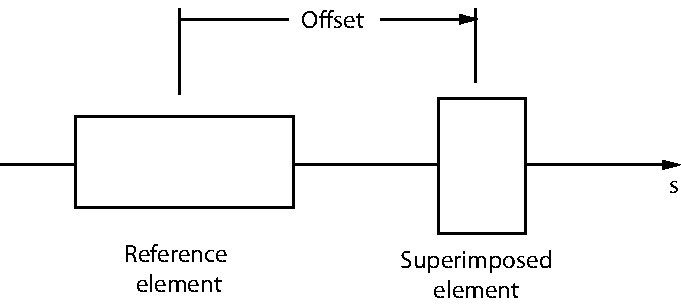
\includegraphics{superimpose.pdf} 
\caption[Superposition Illustration.]
{Illustration of a superposition.}
\label{f:superimpose}
\end{figure}

With the lattice broken up like this \bmad has constructed something
that can be easily analyzed. However, the original elements \vn{Q} and
\vn{S} still exist within the lord section of the lattice. \bmad has
bookkeeping routines so that if a change is made to the \vn{Q} or
\vn{S} elements then these changes can get propagated to the
corresponding slaves. It does not matter which element is
superimposed. Thus, in the above example, \vn{S} could have been put
in the Beam Line (with a drift before it) and \vn{Q} could then have
been superimposed on top and the result would have been the same
(except that the split elements could have different names).

Superpositions are restricted in that \bmad may not have an
appropriate element for the superimposed fields. For example, a
solenoid can not be superimposed over an octupole. If a zero length
element, such as a marker, is superimposed with some other element (or
vice versa) the element is just split in two. For example:
\begin{example}
  Q: quad, l = 10
  M: marker, superimpose, offset = 6
  lat: line = (Q)
  use, lat
\end{example}
The resulting is that the tracking part of the lattice would be
\begin{example}
        Element   Key           Length
  1)    Q{\#}1       Quadrupole    6
  2)    M         Marker        0
  3)    Q{\#}2       Quadrupole    4
\end{example}
and the lord part of the lattice would have the \vn{Q} element.
 
A superposition is illustrated in Figure~\ref{f:superimpose} The
placement of a superimposed element is determined by three factors: A
reference point on the superimposed element, a reference point in the
lattice line, and an offset between the points. The attributes that
determine these three quantities are: 
\index{ref}\index{offset}
\index{ref_beginning}\index{ref_center}\index{ref_end}
\index{ele_beginning}\index{ele_center}\index{ele_end}
\begin{example}
  ref = <element name in lattice>
  offset = <length>      (default = 0)
  ref_beginning
  ref_center             (default)
  ref_end
  ele_beginning
  ele_center             (default)
  ele_end
\end{example}
\vn{ref} sets the reference element. If \vn{ref} is not present then
the start of the lattice is used. \vn{ref_beginning}, \vn{ref_center}
or \vn{ref_end} can be used to indicate where on the reference element
the reference point is. Default is \vn{ref_center}. Similarly,
\vn{ele_beginning}, \vn{ele_center}, or \vn{ele_end} can be used to
indicate the reference point on the superimposed element at the
beginning (entrance) edge, the center, or the end (exit) edge
respectively. If neither of these attributes are given the default is
to use the element center. \vn{offset} is the longitudinal offset
between the reference point on the reference element and the reference
point on the superimposed element. The default if not present is zero.

\index{lattice_type}
\index{linear_lattice}
\index{drift}
\index{overlay}
\index{group}
\index{girder}
Superposition may be done with any element except \vn{Drift},
\vn{Group}, \vn{Overlay}, and \vn{Girder} control elements. A
superimposed element that extends beyond either end of the lattice
will be wrapped around so part of the element will be at the beginning
of the lattice and part of the element will be at the end. For
consistency's sake, this is done even if the \vn{lattice_type} is set
to \vn{linear_lattice} (for example, it is sometimes convenient to
treat a circular lattice as linear). Example:
\begin{example}
  d: drift, l = 10
  q: quad, l = 2, superimpose
  machine: line = (d)
  use, machine
\end{example}
The lattice will have three elements in the tracking section:
\begin{example}
        Element   Key           Length
  3)    Q{\#}2       Quadrupole    1
  2)    D{\#}1       Drift         8
  1)    Q{\#}1       Quadrupole    1
\end{example}
The lord section of the lattice will have the element \vn{Q}. 

When a superposition is made that overlaps a drift the drift, not
being a "real" element, vanishes. That is, it does not get put in the
lord section of the lattice. Thus, it is an error if a second
superposition uses the drift as the reference element. For example
\begin{example}
  dft1: drift, l = 10
  q1: quad, l = 1, superposition, ref = dft1   ! OK 
  q2: quad, l = 2, superposition, ref = dft1   ! ERROR! 
\end{example}
Also note that if aperture limits (\sref{s:limit}) have been assigned
to a drift, the aperture limits can ``disappear'' when the
superposition is done. Explicitly, if the exit end of a drift has been
assigned aperture limits, the limits will disappear if the
superimposed element overlays the exit end of the drift. A similar
situation applies to the entrance end of a drift.

%-----------------------------------------------------------------------------
\subsection{Changing Element Lengths when there is Superposition}
\label{s:super.length}

\index{overlay}
\index{group}
\index{expand_lattice}
When the lattice is constructed, superposition of elements is done
before the addition of any \vn{group} or \vn{overlay} elements. This
is done since \vn{overlay}s and \vn{group}s are allowed to refer
to elements that are superimposed. This can lead to some unexpected
results. For example:
\begin{example}
  q1: quad, l = 10
  q2: quad, l = 10
  lat: line = (q1, q2)
  use, lat
  o: overlay = {q1}, l = 12
  m: marker, superimpose, offset = 15
\end{example} 
In this example, the marker is initially positioned at 15~meters.
The application of the overlay will increase the length of \vn{q1} by
2~meters which will push the marker \vn{m} to 17~meters which is probably 
not what was intended. To avoid this problem, an \vn{expand_lattice} statement
(\sref{s:expand}) can be placed after the overlay, but before the
superimpose, statement
\begin{example}
  ...
  o: overlay = {q1}, l = 12
  expand_lattice
  m: marker, superimpose, offset = 15
\end{example} 

The length of a superimposed element must necessarily be equal to the
sum of the lengths of its slave elements. For example, the element
\vn{S} in the first example of Section~\sref{s:super} has a length of
6~meters which is equal to the sum of the length of \vn{Q{\B}S}
(3~meters) plus the length of \vn{S{\#1}} (also 3~meters).

If a program varies the length of a superimposed element after the
lattice has been parsed, the length of the slaves will be adjusted
accordingly. For example, if element \vn{S} in the first example
of Section~\sref{s:super} is increased from 6~meters to 9~meters, the
lattice would look like
\begin{example}
        Element   Key         Length  Total
  1)    Q{\#}1       Quadrupole   4        4
  2)    Q{\B}S       Sol_quad     6       10
  3)    S{\#}1       Solenoid     3       13
  4)    D{\#}2       Drift        8       21
\end{example}
The length of \vn{Q{\B}S} has been increased from 4~meters to 6~meters
and the length of \vn{S{\#}1} has been increased from 2~meters to
3~meters to give the proper length for \vn{S}. Additionally, to keep
the length of \vn{Q} at 10~meters, the length of \vn{Q{\#}1} has been
decreased to 4~meters. Notice that the overall length of the lattice
has increased by 1~meter. 

Notice that this result is {\em not} what would be obtained if the
length of the element \vn{S} is increased to 9~meters in the lattice
file. The reason for this incompatibility stems from the fact that, in
general, it is a complex problem to have length changes after parsing
mirror what would happen if the lengths were changed in the lattice
file itself. As a result, \bmad chooses to use a relatively simple
algorithm. In practice, lattice layouts can be designed without
superimpose, using the \vn{no_superimpose} command (\sref{s:no.superimpose}), and when the
element lengths are fixed, superposition can be used.


%-----------------------------------------------------------------------------
\section{Multipass}
\label{s:multipass}
\index{multipass|hyperbf}

Some lattices have the beam recirculating through the same element
multiple times. For example, an Energy Recovery Linac (ERL) will
circulate the beam back through the LINAC part to retrieve the energy
in the beam. In \bmad this situation can simulated using the
\vn{multipass} attribute. A simple example shows how this works.
\index{expand_lattice}
\begin{example}
  A: lcavity
  linac_part: line[multipass] = (A, ...)
  my_line: line = (linac_part, ..., linac_part)
  use, my_line
  expand_lattice
  A\B2[dphi0] = 0.5
\end{example}
The tracking part of the lattice consists of two slave elements
\begin{example}
  A\B1, ..., A\B2, ...
\end{example}
Since the two elements are derived from a \vn{multipass} line they are
given unique names by adding a \vn{{\B}n} suffix. In addition there is
a lord element (that doesn't get tracked through) called \vn{A} in the
lord part of the lattice. Changes to attributes of the lord \vn{A}
element will be passed to the slave elements by \bmad's bookkeeping
routines. Assuming \vn{A\B1} is an accelerating cavity, to make
\vn{A\B2} a decelerating cavity the \vn{dphi0} attribute of
\vn{A\B2} is set to 0.5. This is the one attribute that \bmad's
bookkeeping routines will not touch when transferring attribute values
from \vn{A} to its slaves. Notice that the \vn{dphi0} attribute had to
be set after \vn{expand_lattice} (\sref{s:expand})
is used to expand the lattice since
\bmad does immediate evaluation and \vn{A\B2} does not exist before
the lattice is expanded.

Sublines of a multipass line are automatically multipass:
\begin{example}
  a_line: line = (...)
  m_line: line[multipass] = (..., a_line, ...)
\end{example}
In this example \vn{a_line} is implicitly multipass.

Multiple elements of the same name in a multipass line are considered 
physically distinct:
\begin{example}
  m_line: line[multipass] = (A, A, B)
  u_line: line = (m_line, m_line)
  use, u_line
\end{example}
In this example the tracking part of the lattice is
\begin{example}
  A\B1, A\B1, B\B1, A\B2, A\B2, B\B2
\end{example}
In the control section of the lattice there will be two multipass
lords called \vn{A} and one called \vn{B}. The first \vn{A} lord 
controls the 1\St and 4\Th elements in the tracking part of the lattice 
and the second \vn{A} lord controls the 2\Nd and 5\Th elements.

If a multipass line is reversed then the elements are considered to be
transversed backwards:
\begin{example}
  m_line: line[multipass] = (A, A, B)
  u_line: line = (m_line, -m_line)
  use, u_line
\end{example}
In this example the tracking part of the lattice is
\begin{example}
  A\B1, A\B1, B\B1, B\B2, A\B2, A\B2
\end{example}
Here the 1\St and 6\Th elements are connected to a multipass lord and the
2\Nd and 5\Th elements are connected to a different multipass lord.

%-----------------------------------------------------------------------------
\subsection{The Reference Orbit in a Multipass Line}

\index{lcavity}
\index{p0c}\index{e_tot}
If there are \vn{lcavity} elements in the lattice then the reference
energy at a given element may differ from pass to pass. In this case,
the normalized strength (k1, kick, etc.) for magnetic and electric
elements will not be the same from pass to pass. To avoid an
ambiguity, all magnetic and electric elements that are used in a
multipass line must have their magnetic or electric field strength set
as the independent attribute (\sref{s:depend}), {\em or} a reference
energy (\sref{s:energy}) must be defined. A reference energy is
defined by setting \vn{e_tot} or \vn{p0c}, or by setting
\vn{n_ref_pass} as described below. 

\begin{figure}[tb]
\centering 
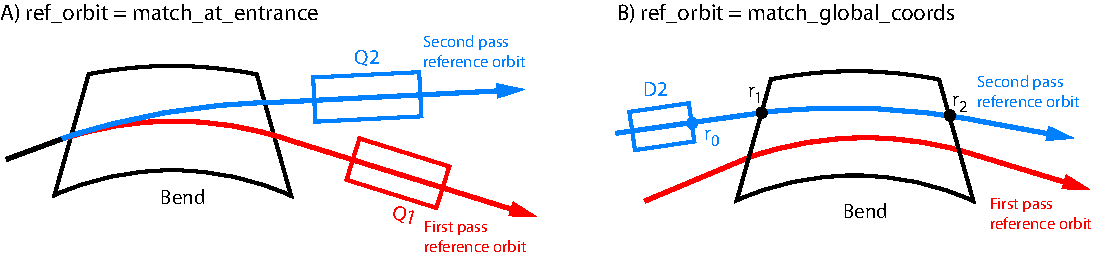
\includegraphics[width=6.2in]{multipass_bend.pdf} 
\caption[The reference orbit with a multipass bend.]  
{A) With \vn{ref_orbit} = \vn{match_at_entrance}, the reference orbits
of different pass will be taken to be the same at the entrance end of
the magnet. If there is a variation of the reference energy through a
bend from pass to pass, the reference orbit through the bend will vary
from pass to pass. B) With \vn{ref_orbit} = \vn{match_global_coords},
the reference orbit on the first pass establishes the position of the
bend in the global coordinate system and the reference orbit on other
passes is calculated with respect to this.}
\label{f:multipass.bend}
\end{figure}

\index{sbend}\index{rbend}\index{patch}
For a bend in a multipass line, there is the added complication of how
to define the reference orbit when the reference energy is different
from pass to pass. If, say, a different reference orbit is used for
each pass there is a problem of how to interpret multipole values
like \vn{k1}. On the other hand, it is sometimes very convenient to be
able to use separate reference orbits. 

A bend element has a \vn{ref_orbit} attribute that, when combined with
the reference energy, define the reference orbit. \vn{ref_orbit} is a
switch that can take the values:
\begin{example}
  single_ref            ! Default. 
  match_global_coords   ! Must be used with n_ref_pass = 1
  match_at_entrance
  match_at_exit
  patch_in              ! Used with patch elements,
  patch_out             !   and must be used with n_ref_pass = 1.
\end{example}
A value of \vn{single_ref} (the default) means that the {\em same}
reference orbit will be used for all passes. The \vn{match_global_coords},
\vn{match_at_entrance} and \vn{match_at_exit} values are used when
{\em separate} reference orbits are desired as described below.

To set the reference energy, one (and only one) of the attributes
\vn{n_ref_pass}, \vn{e_tot} or \vn{p0c} needs to be
set. \vn{n_ref_pass} is an integer indicating which pass is used to
define the reference energy for the lord element. Note: If
\vn{ref_orbit} is set to \vn{match_global_coords}, \vn{n_ref_pass} must be
used and must be set to 1.

An example will make this clear. Consider a bend defined by
\begin{example} 
  B: sbend, l = 1, b_field = 1.0, n_ref_pass = 1, ref_orbit = single_ref
\end{example}
Here the same reference orbit will be used for all passes. Assume that
the reference momentum \vn{p0c} on the first pass is 5~GeV (this is
determined by the reference momentum at the beginning of the lattice
and any \vn{lcavity} elements in the lattice). Since \vn{n_ref_pass}
is one, this fixes the momentum at which the reference orbit is
calculated to be 5~GeV. The bending radius \vn{rho} of the reference
orbit is related to the field and momentum by
\begin{example}
  rho = p0c / (c_light * b_field)
\end{example}
In this case, this translates into a bending radius of 16.7~m. In the
tracking lattice, the first pass element \vn{B\B1} will have a value
for \vn{b_field} of 1~Tesla just like its lord element. Also,
like its lord element, \vn{B\B1} will have an error field,
\vn{b_field_err}, of zero. The total field
\begin{example}
  b_field_tot = b_field + b_field_err
\end{example}
will be 1~Tesla. Additionally, the edge face angles \vn{e1} and
\vn{e2} will be the same as \vn{B}. In this example both are
zero. This is true for all passes.

Now assume that on the second pass, the reference momentum is 10~GeV.
Since, on the second pass, \vn{p0c} is a factor of 2 larger, to keep
the bending radius invariant, the value of \vn{b_field} for the second
pass element \vn{B\B2} will be a factor of 2 larger. That is, it will
be 2~Tesla. However, the total field in the element must be the
same on all passes (\vn{B\B1} and \vn{B\B2} represent the same
physical element after all). Thus, \vn{B\B2} must have a value for
\vn{b_field_err} of -1~Tesla.

Consider the case where the value of
\vn{ref_orbit} is set to \vn{match_at_entrance} and the reference
momentum is set instead of \vn{n_ref_pass}:
\begin{example} 
  B: sbend, l = 1, b_field = 1.0, p0c = 5e9, ref_orbit = match_at_entrance
\end{example}
Here the reference orbit will be different on the two passes. The two
reference orbits will coincide at the entrance edge of the magnet.
This is illustrated in Figure~\ref{f:multipass.bend}A. For both
\vn{B\B1} and \vn{B\B2}, the value of \vn{b_field} will be 1~Tesla
giving bending radii of \vn{16.7}~m and \vn{33.4}~m respectively. With
\vn{B\B2}, the element length will be a slight bit larger than
\vn{B\B1} with a value of \vn{1.0000045}. The entrance face angle
\vn{e1} will always be the same on all passes (zero in this example)
but \vn{e2} will vary. In this case \vn{e2} for \vn{B\B2} will be
\vn{0.003}. With the different reference orbit for the second pass,
there is no good way to handle a non-zero multipole attribute so \bmad
disallows them in this case.

\vn{match_at_exit} is similar to \vn{match_at_entrance} except that
the different reference orbits will coincide at the exit edge of the
magnet. If \vn{match_at_exit} is used with the parameters in the above
example, the only change for \vn{B\B2} is that \vn{e1} will now be
\vn{0.003} and \vn{e2} will be zero.

The \vn{match_at_entrance} value for \vn{ref_orbit} is useful
for simulating a bend at the end of a multipass line that is used to
separate the beams on the various passes. Notice that the next
elements downstream (labeled \vn{Q1} and \vn{Q2} in
Figure~\ref{f:multipass.bend}A) will be physically separated in
space. That is, it does not make sense to use \vn{match_at_entrance}
for a bend that is {\em not} at the end of a multipass
line. Similarly, the \vn{match_at_exit} value is useful for simulating
a bend that combines beams of different energies. Such a bend should
be placed at the beginning of a multipass line.

With \vn{ref_orbit} set to \vn{match_global_coords} the reference
orbit on a given pass is determined by the global coordinates
(\sref{s:global}) of the reference trajectory. Example:
\begin{example} 
  B: sbend, l = 1, b_field = 1.0, n_ref_pass = 1, ref_orbit = match_global_coords
\end{example}
As will be explained, when using \vn{match_global_coords},
\vn{n_ref_pass} must be present and set to 1. With
\vn{match_global_coords}, \vn{B\B1} will have the same parameters as
\vn{B} and this will determine the reference orbit for \vn{B\B1}. See
Figure~\ref{f:multipass.bend}B). For the second pass, the reference
trajectory at the entrance end of the bend is determined as follows:
The calculation starts with the global coordinates of the reference
orbit at the exit end of the element just before \vn{B\B2} (marked
$r_0$ in Figure~\ref{f:multipass.bend}B)). To be physically correct,
this point must lie on the entrance face of \vn{B\B2}. However, it is
possible to have a lattice where this is not so and the calculation
does not demand this. If $r_0$ does not lie on the entrance face, the
reference orbit is extended (either forward or backward) in a straight
line to a point where it intersects the entrance face (marked $r_1$ in
Figure~\ref{f:multipass.bend}B)). The radius of curvature is
calculated by scaling the radius as calculated from the first pass
scaled by the change in reference momentum between the first and
second passes. From the entrance point and the radius of curvature,
the exit point (marked $r_1$ in Figure~\ref{f:multipass.bend}B)) can
be calculated. The curve from $r_1$ to $r_2$ defines the reference
trajectory through \vn{B\B2}. The face angles \vn{e1} and \vn{e2}, and
the path length \vn{l} for \vn{B\B2} can be calculated from the
geometry.

Since the calculation with \vn{match_global_coords} is rather
complicated, the use of \vn{match_global_coords} is restricted to
lattices that lie horizontally in the global $X-Z$ plane. Also, the
restriction to \vn{n_ref_pass = 1} is necessary since the calculation
becomes nondeterministic otherwise. 

Additionally, for a bend, with \vn{ref_orbit} set to
\vn{match_at_entrance}, \vn{match_at_exit} or
\vn{match_global_coords}, the bend must be a pure dipole. That is, no
quadrupole or higher order components. This assumption is
necessary since the reference orbit calculation assumes that the
orbit within the bend is circular for all reference orbits.

%-----------------------------------------------------------------------------
\subsection{Using Patch elements to Vary the Reference Orbit in a Multipass Line}
\label{s:multi.patch}

\begin{figure}[tb]
\centering 
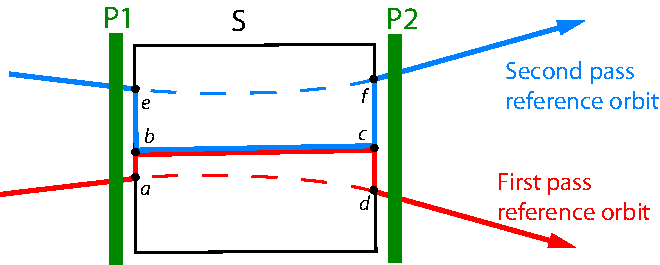
\includegraphics[width=4in]{multipass_patch.pdf} 
\caption[Using patch elements to vary the reference orbit in a multipass line.]
{Using patch elements to vary the reference orbit in a multipass line. 
The gap between \vn{patch} elements \vn{P1} and \vn{P2} and the lattice section 
\vn{S} is for illustration purposes only.
}
\label{f:multipass.patch}
\end{figure}

There exist situations where it is desirable to have a different
reference orbits for each pass through a non-bend elements. Such a
situation is illustrated in Figure~\ref{f:multipass.patch}. In this
example, beams of differing energy pass through an a section of the
lattice labeled \vn{S}. This section may contain one or more
elements. The desired reference orbit for each pass follows the beam
trajectories. This is achieved by placing patch elements, called
\vn{P1} and \vn{P2}, just before and just after \vn{S}. The
corresponding lattice file would look like
\begin{example}
  p1: patch, ref_orbit = patch_in, n_ref_pass = 1, translate_after = True
  p2: patch, ref_orbit = patch_out, n_ref_pass = 1, ref_patch = p1

  m_line: line[multipass] = (p1, S, p2)
  all_line: line = (..., m_line, ..., m_line, ...)
  use, all_line
  
  expand_lattice
  p1\B1[x_offset] = 0.05
  p1\B1[x_pitch] = -0.0034
\end{example}
The \vn{ref_orbit} parameter for \vn{p1} and \vn{p2} indicate whether
the patch is just before (\vn{patch_in}) or just after
(\vn{patch_out}) the section of interest. In this example,
\vn{x_offset} and \vn{x_pitch} parameters for the first pass slave
\vn{p1\B1} are set in the lattice file. This determines the
orientation of the reference orbit through \vn{S} (labeled $b$-$c$ in
the figure) with respect to the incoming first pass reference
orbit. Point $a$ in the figure is the first pass reference orbit just
before \vn{p1\B1} and point $b$ is the reference orbit just after. On
the second pass, \bmad will calculate the patch parameters for
\vn{p1\B2} so that the global coordinates of the reference orbit just
after \vn{p1\B2} is the same as the reference orbit just after
\vn{p1\B1}. That is, point $b$.

The patch parameters for the \vn{p2\B1} first pass slave of \vn{p2},
which has \vn{ref_orbit} set to \vn{patch_out}, the calculation is as
follows: In the definition of \vn{p2} the \vn{ref_patch} parameter is
set to \vn{p1}. \bmad uses this as the starting point for
tracking. \bmad starts with a particle on the reference trajectory
just {\em before} \vn{p1\B1} and tracks it to the end of \vn{S} (curve
$a$-$d$ in the figure). \bmad then sets the parameters of \vn{p2\B1}
so that the reference orbit after the patch (point $d$) coincides
with the particle. The calculation of the second pass slave \vn{p2\B2}
is analogously computed.

The above procedure of defining the reference orbit using patches with
\vn{ref_orbit} set to \vn{patch_in} and \vn{patch_out} is helpful in
designing lattices. However, once a lattice is designed, there will be
a problem for simulations of lattice errors since particle
trajectories, and hence the reference orbit, will be affected by such
errors. To avoid this, once the layout of the lattice has been settled
on, the \vn{patch_in} and \vn{patch_out} patches should be removed and
four new patches, to replace the four multipass slave patches, should
be introduced outside of the multipass section with the patch
parameters set to the appropriate values.

\chapter {Element Attributes}
\label{c:attrib}
\index{element attribute}

%-----------------------------------------------------------------
\section{Dependent and Independent Attributes} 
\label{s:depend} 
\index{element attribute!dependent and independent}

\index{parameter statement}
\index{dependent attribute}
For convenience, \bmad computes the values of some attributes based
upon the values of other attributes. Some of these dependent variables are
listed in Table~\ref{t:dependent}. Also shown in
Table~\ref{t:dependent} are the independent variables they are
calculated from.  In the table \vn{n_part} and \vn{l_lattice} (lattice
length) are lattice attributes, not element attributes. The first two
are set by the \vn{parameter} statement (See
\sref{s:param}). \vn{l_lattice} is calculated when the lattice is read
in.

\index{bbi_constant}\index{charge}\index{sig_x}\index{sig_y}
\index{e_tot}\index{n_part}\index{e_field}\index{voltage}
\index{hkick}\index{vkick}\index{gap}\index{l}
\index{e_tot}\index{e_loss}\index{delta_e}\index{gradient}
\index{l}\index{rho}\index{angle}\index{l_chord}
\index{g}\index{l}\index{k1}\index{rho}\index{num_steps}\index{ds_step}
\index{b_max}\index{e_tot}\index{beambeam}\index{elseparator}
\index{lcavity}\index{rbend}\index{sbend}\index{wiggler}
\begin{table}[ht]
\centering {
\begin{tabular}{|l|l|l|} \hline
 {\em Element}                & {\em Independent Variables}    & {\em Dependent Variables}          \HH
 All elements                 & \vn{ds_step}                   & \vn{num_steps}                     \HH
 \vn{BeamBeam}                & \vn{charge}, \vn{sig_x}, \vn{sig_y}, \vn{e_tot}, \vn{n_part}
                                                               & \vn{bbi_constant}                  \HH
 \vn{Elseparator}             & \vn{hkick}, \vn{vkick}, \vn{gap}, \vn{l}, \vn{e_tot}      
                                                               & \vn{e_field}, \vn{voltage}         \HH
 \vn{Lcavity}                 & \vn{gradient}, \vn{l}          & \vn{e_loss}, \vn{voltage}          \HH
 \vn{Rbend}, \vn{Sbend}       & \vn{g}, \vn{l}                     
                                                               & \vn{rho}, \vn{angle}, \vn{l_chord} \HH

 \vn{Wiggler} (map type)      & \vn{term(i)}                   & \vn{b_max}, \vn{k1}, \vn{rho}      \HH
 \vn{Wiggler} (periodic type) & \vn{b_max}, \vn{e_tot}         & \vn{k1}, \vn{rho}                  \HH
\end{tabular}
}
\caption[Table of dependent variables.]{Partial listing of dependent variables and 
  the independent variables they are calculated from.}
\label{t:dependent}
\end{table}

\index{lattice!expansion}\index{harmon}\index{delta_e}\index{gradient}
\index{rho}\index{g}\index{angle}\index{rf_frequency}
No attempt should be made to set or vary within a program dependent
attributes. It should be remarked that this is not an iron clad rule.
If a program properly bypasses \bmad's attribute bookkeeping routine
then anything is possible. In a lattice file, before lattice expansion
(\sref{s:expand}), \bmad allows the setting of a select group of
dependent attributes if the appropriate independent attributes are
not set. The list of settable dependent variables is given in
Table~\ref{t:dep.except}.  After reading in the lattice \bmad will set
the appropriate independent variable based upon the value of the
dependent variable. \vn{harmon} is the exception in that it will never
be set by the bookkeeping routine.
\index{lcavity}\index{rbend}
\index{sbend}\index{rfcavity}
\begin{table}[ht]
\centering {
\begin{tabular}{|l|l|l|} \hline
{\em Element}                  & {\em Dependent Variable Set}  &  {\em Independent Variables Not Set} \HH
  \vn{Lcavity}                 & \vn{voltage}       & \vn{gradient}      \HH
  \vn{Rbend}, \vn{Sbend}       & \vn{rho}           & \vn{g}             \HH
  \vn{Rbend}, \vn{Sbend}       & \vn{angle}         & \vn{g}, or \vn{l}  \HH
  \vn{RFcavity}                & \vn{rf_frequency}  & \vn{harmon}        \HH
  \vn{Wiggler} (periodic type) & \vn{n_pole}        & \vn{l_pole}        \HH
\end{tabular}
}
\caption {Dependent variables that can be set in a primary lattice file.}
\label{t:dep.except}
\end{table}

\index{g}\index{g_err}\index{b_field}\index{bs_field}\index{b_field_err}
\index{b1_gradient}\index{b2_gradient}\index{b3_gradient}\index{ks}
\index{k1}\index{k2}\index{k3}
\index{bl_kick}\index{bl_hkick}\index{bl_vkick}
\index{kick}\index{hkick}\index{vkick}
The normal attribute used to vary the strength of, say, a
\vn{quadrupole} is \vn{k1}.  It is sometimes convenient to be able to
vary the magnetic field strength directly instead. To do this \bmad
has a rule that if the appropriate field attribute appears in the
primary lattice file then it becomes an independent variable and the
normalized strength attribute (the strength attribute normalized by
the reference energy) becomes a dependent variable as tabulated in
Table~\ref{t:dep.field}.
\index{sbend}\index{rbend}\index{solenoid}\index{quadrupole}
\index{sol_quad}\index{sextupole}\index{octupole}
\begin{table}[ht]
\centering {
\begin{tabular}{|l|l|l|} \hline
  {\em Element} & {\em Normalized Strength} & {\em Field Attribute} \HH
  \vn{Sbend}, \vn{Rbend}     & \vn{g}      &  \vn{b_field}        \HH
  \vn{Sbend}, \vn{Rbend}     & \vn{g_err}  &  \vn{b_field_err}    \HH
  \vn{Solenoid, Sol_quad}    & \vn{ks}     &  \vn{bs_field}       \HH
  \vn{Quadrupole, Sol_quad, Sbend, Rbend}            
                             & \vn{k1}     &  \vn{b1_gradient}    \HH
  \vn{Sextupole, Sbend, Rbend}             
                             & \vn{k2}     &  \vn{b2_gradient}    \HH
  \vn{Octupole}              & \vn{k3}     &  \vn{b3_gradient}    \HH
  \vn{HKicker}, \vn{VKicker} & \vn{kick}   &  \vn{bl_kick}        \HH
  Most                       & \vn{hkick}  &  \vn{bl_hkick}       \HH
  Most                       & \vn{vkick}  &  \vn{bl_vkick}       \HH
\end{tabular}
}
\caption {Field and Strength Attributes.}
\label{t:dep.field}
\end{table}
Using both field strength and normalized strength as the independent
variable for a given element is not permitted. For example, for a quadrupole the 
normalized strengths \vn{k1}, \vn{hkick}, and \vn{vkick} can be used as the
independent variable or the field strengths \vn{b1_gradient}, \vn{bl_hkick} and
\vn{bl_vkick}. but the mixing of the two is not valid
\begin{example}
  Q1: quadrupole, k1 = 0.6, bl_hkick = 37.5  ! NO. Not VALID.
\end{example}
\index{field_master}
To define an element with the field strength as the independent
attribute without setting the strength just set the strength to zero
or, alternatively, the \vn{field_master} logical can be set. For
example
\begin{example}
  Q1: quadrupole, b1_gradient = 0   ! Field strengths now the independent variables
  Q1: quadrupole, field_master = T  ! Same as above
\end{example}
The same effect can be obtained by setting the field or \vn{field_master} attributes
after the element has been defined.
\begin{example}
  q1: quadrupole        ! Define q1.
  q1[b1_gradient] = 0   ! Field strengths now the independent variables.
  q1[field_master] = T  ! Same as above.
\end{example}

%-----------------------------------------------------------------
\section{Type, Alias and Descrip Attributes}
\label{s:alias}
\index{type|hyperbf}
\index{alias|hyperbf}
\index{descrip|hyperbf}

There are three string labels associated with any element:
\begin{example}
  type    = <String>
  alias   = <String>
  descrip = <String>
\end{example}
\bmad routines do not use these labels except when printing element
information. \vn{type} and \vn{alias} can be up to 40 characters in
length and \vn{descrip} can be up to 200 characters. The attribute
strings can be enclosed in double quotation marks ("). The attribute
strings may contain blanks. If the attribute string does not contain a
blank then the quotation marks may be omitted. In this case the first
comma (,) or the end of the line marks the end of the string. Example:
\begin{example}
  Q00W: Quad, type = "My Type", alias = Who_knows, &
                                  descrip = "Only the shadow knows"
\end{example}

%-----------------------------------------------------------------
\section[Energy and Wavelength Attributes]{Energy and Wavelength Attributes: E_tot, P0C, and \\ ref_wavelength }
\label{s:energy}
\index{parameter statement}\index{e_tot}
\index{e_tot_start}\index{p0c_start}
\index{patch}\index{lcavity}\index{p0c}\index{e_gun}
\index{n_ref_pass}\index{ref_wave_length}
The attributes that define the reference energy and momentum at an element are:
\begin{example}
  e_tot  = <Real>  ! Total energy in eV.
  p0c    = <Real>  ! Momentum in eV.
\end{example}
The energy and momentum are defined at the exit end of the element.
For ultra--relativistic particles, and for photons, these two values
are the same (\sref{s:phase.space}). Except for multipass elements
(\sref{s:multipass}), \vn{e_tot} and \vn{p0c} are dependent attributes
and, except for multipass elements, any setting of \vn{e_tot} and
\vn{p0c} in the lattice input file is an error. The value of
\vn{e_tot} and \vn{p0c} for an element is calculated by \bmad to be
the same as the previous element except for \vn{e_gun}, \vn{lcavity} and
\vn{patch} elements. To set the \vn{e_tot} or \vn{p0c} at the start of
the lattice use the \vn{beginning} or \vn{parameter} statements.
See~\sref{s:param}. Since the energy changes from the start to the end
of an \vn{lcavity} or. \vn{em_field}, an \vn{lcavity} or \vn{em_field} has
the dependent attributes
\index{em_field}\index{lcavity}
\begin{example}
  e_tot_start   and
  p0c_start
\end{example}
which are just the reference energy and momentum at the start of the element.

\index{init_ele}
The \vn{init_ele} element (\sref{s:init.ele}) also has associated
\vn{e_tot_start} and \vn{p0c_start} attributes as well as \vn{e_tot}
and \vn{p0c}. Generally, for an \vn{init_ele}, \vn{p0c_start} and
\vn{p0c} are the same and \vn{e_tot_start} and \vn{e_tot} are the same
and the values for these attributes are set in the lattice file with
the appropriate \vn{parameter} (\sref{s:param}) or \vn{beginning}
(\sref{s:beginning}) statement. The exception occurs when there is an
\vn{e_gun} element in the lattice (\sref{s:e.gun}). In this case, the
\vn{p0c_start} and \vn{e_tot_start} attributes of the \vn{init_ele}
are set to the values as set in the lattice file and \vn{e_tot} is set
to
\begin{example}
  e_tot = e_tot_start + voltage
\end{example}
and \vn{p0c} is calculated from \vn{e_tot} and the mass of the
particle being tracked. For example, if the lattice file contained:
\begin{example}
  beginning[p0c] = 0
  gun: e_gun, voltage = 0.5e6
  injector: line = (gun, ...)
\end{example}
Then the following energy values will be set for the beginning \vn{init_ele} element:
\begin{example}
  p0c_start   = 0
  e_tot_start = mc2
  e_tot       = mc2 + 0.5e6
  p0c         = Sqrt(e_tot - mc2^2)
\end{example}
where \vn{mc2} is the particle rest mass.  The reason for using this
convoluted convention is to allow the setting, in the lattice file, of
a zero reference momentum at the start of the lattice, while
avoiding the calculational problems that would occur if the \vn{e_gun}
element truly had a starting reference momentum of zero.
Specifically, the problem with zero reference momentum is that the
phase space momentum would be infinity as can be seen from \Eqs{ppp}.

For \vn{multipass} elements, the reference energy is set by specifying
one of \vn{e_tot}, \vn{p0c}, or \vn{n_ref_pass} as described in
\sref{s:multipass}.

For photons, the reference wavelength, \vn{ref_wavelength} is also a
dependent attribute calculated from the reference energy.

\vfill

%-----------------------------------------------------------------
\section{Orientation: Offset, Pitch, Tilt, and Roll Attributes}
\label{s:offset}
\index{x_offset|hyperbf}
\index{y_offset|hyperbf}\index{z_offset|hyperbf}
\index{x_pitch|hyperbf}\index{y_pitch|hyperbf}
\index{roll|hyperbf}\index{tilt|hyperbf}

By default, an element, like a quadrupole, is aligned in space
coincident with the reference orbit running through it
(\sref{s:ref.construct}). A quadrupole can be displaced in space using
the quadrupole's ``\vn{orientational}'' attributes. For a quadrupole,
the orientational attributes only affect the physical element and not
the reference orbit. However, the orientational attributes of some
other elements, like the \vn{fiducial} element, do affect the
reference orbit. To sort all this out, lattice elements can be divided
into six classes:
  \begin{description}
  \item[\vn{Straight line elements}] \Newline
Straight line elements are elements where the reference orbit is a
straight line. Examples include \vn{quadrupoles}, and \vn{sextupoles}
as well as zero length elements like \vn{markers}.
  \item[\vn{Dipole bends}]  \Newline
Dipole bends are:
\begin{example}
  sbend \& rbend             ! \sref{s:bend}
\end{example}
  \item[\vn{Photon reflecting elements}] \Newline
The reflecting elements are
\begin{example}
  crystal                   ! \sref{s:crystal}
  mirror                    ! \sref{s:mirror}
  multilayer_mirror         ! \sref{s:multilayer}
\end{example}
These elements have a kink in the reference orbit at the nominal
element surface.
  \item[\vn{Reference orbit manipulator elements}] \Newline
Elements that are used to manipulate the reference orbit are
\begin{example}
  branch \& photon_branch    ! \sref{s:branch}
  floor_shift               ! \sref{s:floor.ele}
  patch                     ! \sref{s:patch}
\end{example}
  \item[\vn{Fiducial Element}] \Newline
  \item[\vn{Girder Elements}] \Newline
  \item[\vn{Control Elements}] \Newline
Control elements are elements that control attributes of other
elements. The control elements are:
\begin{example}
  group
  overlay
\end{example}
These elements do not have orientational attributes.
  \end{description}

%-----------------------------------------------------------------
\subsection{Straight Line Element Orientation}

The straight line elements have the following orientational attributes:
\begin{example}
  x_offset = <Real>
  y_offset = <Real>
  z_offset = <Real>
  x_pitch  = <Real>
  y_pitch  = <Real>
  tilt     = <Real>    
\end{example}
For straight line elements the orientational attributes only shift the
physical element and do not affect the reference orbit.

\begin{figure}[tb]
  \centering
  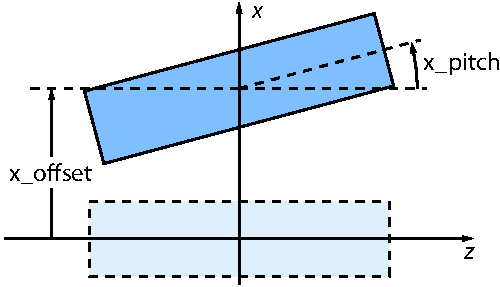
\includegraphics{pitch.pdf}
  \caption{Geometry of Pitch and Offset attributes}
  \label{f:pitch}
\end{figure}

\vn{x_offset} translates an element in the local $x$--direction
as shown in \fig{f:pitch}. Similarly, \vn{y_offset} and 
\vn{z_offset} translate an element along the local $y$ and 
$z$--directions respectively.

The \vn{x_pitch} attribute rotates an element about the element's
center such that the exit face of the element is displaced in the
$+x$--direction as shown in figure~\ref{f:pitch}.  An
\vn{x_pitch} represents a rotation around the positive $y$-axis.

Similarly, the \vn{y_pitch} attribute rotates an element about the
element's center using the negative $x$--axis as the rotation axis so
that the exit face of the element is displaced in the $+y$--direction.

The \vn{x_pitch} and \vn{y_pitch} rotations are about the center of
the element which is in contrast to the \vn{dtheta} and \vn{dphi}
misalignments of \mad which rotate around the entrance point. The
sense of the rotation between \bmad and MAD is:
\index{MAD!element rotation origin}
\begin{example}
  x_pitch (Bmad) =  dtheta (MAD)
  y_pitch (Bmad) = -dphi (MAD)
\end{example}

\begin{figure}[tb]
  \centering
  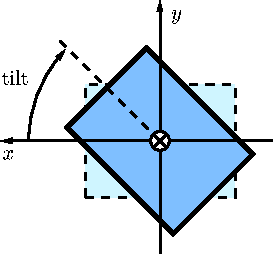
\includegraphics{tilt.pdf}
  \caption{Geometry of a Tilt}
  \label{f:tilt}
\end{figure}

The tilt attribute rotates the element in the $(x, y)$ plane as shown
in figure~\ref{f:tilt}. The rotation axis is the positive
$z$-axis. For example
\begin{example}
  q1: quad, l = 0.6, x_offset = 0.03, y_pitch = 0.001, tilt
\end{example}
\index{sol_quad!tilt default}\index{quadrupole!tilt default}
\index{sextupole!tilt default}\index{octupole!tilt default}
Like MAD, \bmad allows the use of the \vn{tilt} attribute without a
value to designate a skew element. The default tilt is $\pi/(2(n+1))$
where $n$ is the order of the element:
\begin{example}
  sol_quad       n = 1
  quadrupole     n = 1
  sextupole      n = 2
  octupole       n = 3
\end{example}

Note that \vn{hkick} and \vn{vkick} attributes are not affected by
\vn{tilt} except for \vn{kicker} and \vn{elseparator} elements.

%-----------------------------------------------------------------
\subsection{Bend Element Orientation}

\begin{figure}[ht]
  \centering
  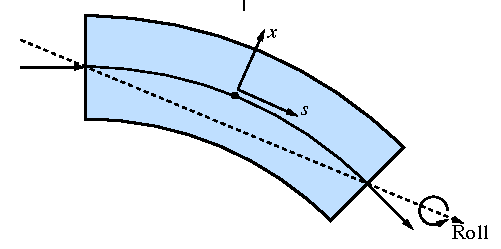
\includegraphics{roll.pdf}
  \caption[Geometry of a Bend]{
Geometry of a Bend. Like straight line elements, offsets and pitches
are calculated with respect to the coordinates at the center of the
bend. The exception is the \vn{roll} attribute which is a rotation
around the axis passing through the entrance and exit points.  Shown
here is the geometry for a bend with \vn{ref_tilt} = 0. That is, the bend
is in the $x-z$ plane.}
  \label{f:roll}
\end{figure}

The orientation attributes for \vn{sbend} and \vn{rbend} elements is
\begin{example}
  x_offset = <Real>
  y_offset = <Real>
  z_offset = <Real>
  x_pitch  = <Real>
  y_pitch  = <Real>
  ref_tilt = <Real>    ! Shifts and reference orbit rotation axis.
  roll     = <Real>    
\end{example}
The geometry for orienting a bend is shown in \fig{f:roll}. Like
straight line elements, the offset and pitch attributes are evaluated
with respect to the center of the element. 

Unlike the straight line elements, bends do not have a \vn{tilt}
attribute. Rather they have a \vn{ref_tilt} and a \vn{roll} attribute.
The \vn{roll} attribute rotates the bend along an axis that runs
through the entrance point and exit point as shown in
figure~\ref{f:roll}. A \vn{roll} attribute, like the offset and pitch
attributes does not affect the reference orbit.
The major effect of a \vn{roll} is to give a vertical
kick to the beam. For a bend with positive bend angle, a positive
\vn{roll} will move the outside portion ($+x$ side) of the bend upward
and the inside portion (-$x$ side) downward. Much like car racetracks
which are typically slanted towards the inside of a turn.

The \vn{ref_tilt} attribute of a bend rotates the bend about the $z$
axis at the upstream end of the bend as shown in \fig{f:roll}. Unlike
\vn{rolls} and \vn{tilts}, \vn{ref_tilt} also shifts the rotation axis
of the reference orbit along with the physical element. A \vn{bend}
with a \vn{ref_tilt} of $\pi/2$ will bend a beam vertically downward
(\sref{s:global}). Note that the \vn{ref_tilt} attribute of \bmad is
the same as the MAD \vn{tilt} attribute.

%-----------------------------------------------------------------
\subsection{Photon Reflecting Element Orientation}

\begin{figure}[ht]
  \centering
  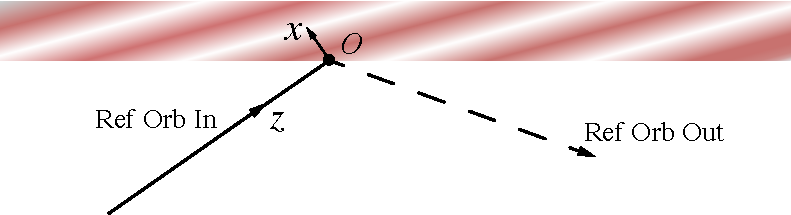
\includegraphics{reflect-orient.pdf}
  \caption[Geometry of a photon reflecting element orientation]{
Geometry of a photon reflecting element orientation.
The reference coordinates used for defining the orientational attribute
is the entrance reference coordinates. 
}
  \label{f:reflect.orient}
\end{figure}

Photon reflecting elements have the following orientational attributes:
\begin{example}
  x_offset = <Real>
  y_offset = <Real>
  z_offset = <Real>
  x_pitch  = <Real>
  y_pitch  = <Real>
  ref_tilt = <Real>    ! Shifts both element and reference orbit.
  tilt     = <Real>    
\end{example}
Roughly, these elements can be viewed as zero length bends except,
since there is no center position, the orientational attributes are
defined with respect to the entrance coordinates as shown in
\fig{f:reflect.orient}. Like bend elements, the \vn{ref_tilt} attribute
rotates both the physical element and the reference coordinates.
The \vn{tilt} attribute rotates just the physical element. Thus
the total rotation of the physical element about the entrance $z$
axis is the sum \vn{tilt} + \vn{ref_tilt}.

%-----------------------------------------------------------------
\subsection{Reference Orbit Manipulator Element Orientation}

The \vn{branch}, \vn{photon_branch}, \vn{floor_shift}, and \vn{patch} elements
use the following attributes to orient their exit edge with respect to their
entrance edge:
\begin{example}
  x_offset = <Real>
  y_offset = <Real>
  z_offset = <Real>
  x_pitch  = <Real>
  y_pitch  = <Real>
  tilt     = <Real>    
\end{example}
Here "exit" edge for \vn{branch} and \vn{photon_branch} elements is defined
to be the start of the line being branched to. [Within the line containing
the branch, the branch is considered to have zero length so the exit face
in the line containing the branch is coincident with the entrance face.]
The placement of the exit edge for these elements defines the reference orbit.
Thus, unlike the corresponding attributes for other elements, 
the orientational attributes here directly control the reference orbit.

%-----------------------------------------------------------------
\subsection{Fiducial Element Orientation}

The \vn{fiducial} element (\sref{s:girder}) uses the 
following attributes to define its position:
\begin{example}
  origin_ele        = <Name>     ! Reference element.
  origin_ele_ref_pt = <location> ! Reference pt on reference ele.
  dx_origin         = <Real>     ! x-position offset
  dy_origin         = <Real>     ! y-position offset
  dz_origin         = <Real>     ! z-position offset
  dtheta_origin     = <Real>     ! orientation angle offset.
  dphi_origin       = <Real>     ! orientation angle offset.
  dpsi_origin       = <Real>     ! orientation angle offset.
\end{example}
See Section~\sref{s:fiducial} for more details.



%-----------------------------------------------------------------
\subsection{Girder Orientation}

A \vn{girder} (\sref{s:girder}) element uses the same attributes as a \vn{fiducial}
element (\sref{s:fiducial}) to orient the reference girder position. In addition,
the following attributes are used to move the girder physically from the reference position: 
\begin{example}
  x_offset = <Real>
  y_offset = <Real>
  z_offset = <Real>
  x_pitch  = <Real>
  y_pitch  = <Real>
  tilt     = <Real>    
\end{example}
Shifting the girder from its reference position shifts all the elements that are
supported by the girder. See Section~\sref{s:girder} for more details.

\index{x_offset_tot|hyperbf}\index{y_offset_tot|hyperbf}\index{z_offset_tot|hyperbf}
\index{x_pitch_tot|hyperbf}\index{y_pitch_tot|hyperbf}
\index{tilt_tot|hyperbf}\index{roll_tot|hyperbf}\index{tilt_err_tot|hyperbf}
If an element is supported by a \vn{girder} element (\sref{s:girder}),
the orientational attributes of the element are with respect to the
orientation of the \vn{girder}. The computed offsets, pitches and tilt with
respect to the local reference coordinates are stored in the dependent attributes
\begin{example}
  x_offset_tot
  y_offset_tot
  z_offset_tot
  x_pitch_tot
  y_pitch_tot
  tilt_tot
  roll_tot
\end{example}
\index{sbend}\index{rbend}
A \vn{*_tot} attribute will only be present if the corresponding non
\vn{*_tot} attribute is present. For example, only \vn{sbend} and
\vn{rbend} elements have a \vn{roll_tot} attribute since only these
elements have a \vn{roll} attribute.

If an element is not supported by a \vn{girder}, the values of the
\vn{*_tot} attributes will be the same value as the values of the
corresponding non \vn{*_tot} attributes.

%-----------------------------------------------------------------
\section{Hkick, Vkick, and Kick Attributes}
\label{s:kick}
\index{hkick|hyperbf}\index{bl_hkick|hyperbf}
\index{vkick|hyperbf}\index{bl_vkick|hyperbf}
\index{kick|hyperbf}\index{bl_kick|hyperbf}


\index{hkicker}
\index{vkicker}
\index{elseparator}
\index{kicker}
The kick attributes that an element may have are:
\begin{example}
  kick,  bl_kick  = <Real>  ! Used only with a Hkicker or Vkicker
  hkick, bl_hkick = <Real>
  vkick, bl_vkick = <Real>
\end{example}
\vn{kick}, \vn{hkick}, and \vn{vkick} attributes are the integrated
kick of an element in radians. \vn{kick} is only used for \vn{hkicker}
and \vn{vkicker} elements. All other elements that can kick use
\vn{hkick} and \vn{vkick}. The \vn{tilt} attribute will only rotate a
kick for \vn{hkicker}, \vn{vkicker}, \vn{elseparator} and \vn{kicker}
elements. This rule was implemented so that, for example, the
\vn{hkick} attribute for a skew quadrupole would represent a
horizontal steering. The \vn{bl_kick}, \vn{bl_hkick}, and
\vn{bl_vkick} attributes are the integrated field kick in
\vn{meters-Tesla}. Normally these are dependent attributes except if
they appear in the lattice file (\sref{s:depend}).

%-----------------------------------------------------------------
\section{Aperture and Limit Attributes}
\label{s:limit}
\index{aperture|hyperbf}
\index{limit|hyperbf}
\index{aperture_at|hyperbf}

\begin{figure}[ht]
  \centering
  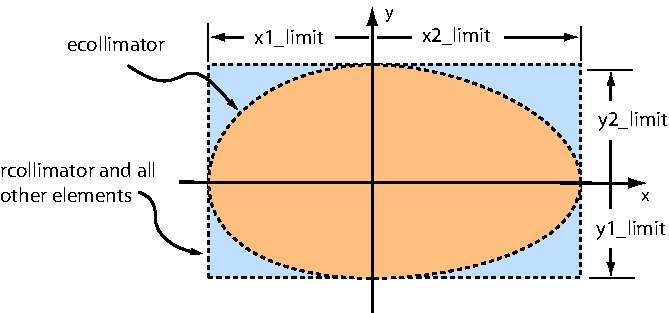
\includegraphics{apertures.pdf}
  \caption[Apertures for ecollimator and rcollimator elements.]
  {Apertures for ecollimator and rcollimator elements. 
  Positive $s$ points up out of the page.}
  \label{f:limit}
\end{figure}

\index{ecollimator}
\index{rcollimator}
\index{x_limit|hyperbf}
\index{y_limit|hyperbf}
\index{x1_limit|hyperbf}
\index{y1_limit|hyperbf}
\index{x2_limit|hyperbf}
\index{y2_limit|hyperbf}
\index{x_offset|hyperbf}
\index{offset_moves_aperture|hyperbf}
\index{aperture_type}
The aperture attributes are:
\begin{example}
  x1_limit      = <Real>      ! Horizontal, negative side, aperture limit
  x2_limit      = <Real>      ! Horizontal, positive side, aperture limit
  y1_limit      = <Real>      ! Vertical, negative side, aperture limit
  y2_limit      = <Real>      ! Vertical, positive side, aperture limit
  x_limit       = <Real>      ! Alternative to specifying x1_limit and x2_limit
  y_limit       = <Real>      ! Alternative to specifying y1_limit and y2_limit
  aperture      = <Real>      ! Alternative to specifying x_limit and y_limit
  aperture_at   = <Switch>    ! What end aperture is at.
  aperture_type = <Switch>    ! What type of aperture it is.
  offset_moves_aperture = <Logical> ! Element offsets affect aperture position
\end{example}
\vn{x1_limit}, \vn{x2_limit}, \vn{y1_limit}, and \vn{y2_limit} specify
the half--width of the aperture of an element as shown in
figure~\ref{f:limit}. A zero \vn{x1_limit}, \vn{x2_limit},
\vn{y1_limit}, or \vn{y2_limit} is interpreted as no aperture in the
appropriate plane.

By default, apertures are assumed to be
rectangular except that an \vn{ecollimator} has a elliptical aperture.
This can be changed by setting the \vn{aperture_type} attribute. The possible 
values of this attribute are:
\begin{example}
  rectangular
  elliptical
  custom
\end{example}
The \vn{custom} setting is used in the case where programs have been
compiled with custom, non-Bmad, code to handle the aperture calculation.

To avoid numerical overflow and other errors in tracking, a particle
will be considered to have hit an aperture in an element, even if
there are no apertures set for that element, if its orbit exceeds 1000
meters. Additionally, there are other situations where a particle will
be considered lost. For example, if a particle's trajectory does
not intersect the output face in a bend.

For convenience, \vn{x_limit} can be used to set \vn{x1_limit} and
\vn{x2_limit} to a common value. Similarly, \vn{y_limit} can be used
to set \vn{y1_limit} and \vn{y2_limit}.  The \vn{aperture} attribute
can be use to set all four \vn{x1_limit}, \vn{x2_limit}, \vn{y1_limit}
and \vn{y2_limit} to a common value. Internally, the \bmad code does {\em not}
store \vn{x_limit}, \vn{y_limit}, or \vn{aperture}. This means that
using \vn{x_limit}, \vn{y_limit} or aperture in arithmetic expressions is
an error:
\begin{example}
  q2: quad, aperture = q1[aperture]   ! THIS IS AN ERROR!
  q2: quad, aperture = q1[x1_limit]   ! Correct
\end{example}

\index{tilt}
\index{x_offset}
\index{y_offset}
\index{x_pitch}
\index{y_pitch}
\index{rcollimator}\index{ecollimator}
\index{multilayer_mirror}\index{mirror}\index{crystal}
Normally, whether a particle hits an aperture or not is evaluated
independent of any element offsets (\sref{s:offset}). This is
equivalent to the situation where a beam pipe containing an aperture
is independent of the placement of the physical element the beam pipe
passes through. That is, the beam pipe does not ``touch'' the physical
element. This can be changed by setting the \vn{offset_moves_aperture}
attribute to \vn{True}. In this case any offsets or pitches will be
considered to have shifted the aperture boundary. The exceptions here
is that the default for the following elements is for
\vn{offset_moves_aperture} to be \vn{True}:
\begin{example}
  rcollimator, 
  ecollimator,
  multilayer_mirror, 
  mirror, and 
  crystal 
\end{example}

Even with \vn{offset_moves_aperture} set to \vn{True}, \vn{tilt}s will
not affect the aperture calculation. This is done, for example, so
that the tilt of a skew quadrupole does not affect the aperture. The
exception here is that tilting an \vn{rcollimator} or \vn{ecollimator}
element will tilt the aperture. Additionally, when the aperture is at
the \vn{surface} (see below), any \vn{tilt} will be used in the
calculation.

\index{both_ends|hyperbf}\index{continuous|hyperbf}
\index{entrance_end|hyperbf}\index{exit_end|hyperbf}
\index{surface|hyperbf}\index{aperture_at}
By default the aperture is evaluated at the exit face only of the
element. This can be changed by setting the \vn{aperture_at} attribute.
Possible settings for \vn{aperture_at} are:
\begin{example}
  entrance_end
  exit_end       ! Default for most elements
  both_ends
  continuous
  surface        ! Default for mirror, multilayer_mirror and crystal
\end{example}
Note that the entrance and exit ends of an element are independent of
which direction particles are tracked through an element. Thus if a
particle is tracked backwards it enters an element at the ``exit end''
and exits at the ``entrance end''. The \vn{continuous} setting
indicates that the aperture is continuous along the length of the
element. This only matters when particle tracking involves stepping
through an element a little bit at a time. For example, as in
Runge-Kutta tracking (\sref{s:tkm}). For tracking where a formula is
used to transform the particle coordinates at the entrance of an
element to the coordinates at the exit end, the aperture is only
checked at the end points so, in this situation, a \vn{continuous}
aperture is equivalent to the \vn{both_ends} setting.

\index{mirror}\index{multilayer_mirror}\index{crystal}
The \vn{surface} setting for \vn{aperture_at} can be only be used for
elements
\begin{example}
  mirror, 
  multilayer_mirror, and 
  crystal
\end{example}
For these elements, the \vn{surface} setting is the default. Due to
the complicated geometry of these elements, to keep things
conceptionally simple, the rule is imposed that, for an aperture at the
surface, the \vn{offset_moves_aperture} setting must be left in its
default state of True. Additionally, For \vn{entrance_end} or
\vn{exit_end} apertures, \vn{offset_moves_aperture} must be set to
False.

Examples:
\begin{example}
  q2: quad, aperture_type = elliptical, aperture_at = continuous
  q1: quad, l = 0.6, x1_limit = 0.045, offset_moves_aperture = T
  q1[y1_limit] = 0.03
  q1[y2_limit] = 0.03
  q1[y_limit] = 0.03  ! equivalent to the proceeding 2 lines.  
  q1[aperture_at] = both_ends
\end{example}

%-----------------------------------------------------------------

\begin{figure}[tb]
  \centering
  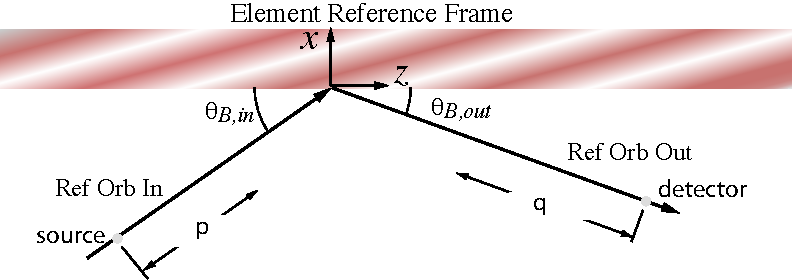
\includegraphics[width=5in]{surface-curvature.pdf}
  \caption[Surface curvature geometry.]
{Surface curvature geometry. The element reference frame used to
describe surface curvature has the $x$ axis pointing towards the
interior of the element, and the $z$ axis along the plane defined by
the entrance and exit reference orbit.}
  \label{f:surface}
\end{figure}

%-----------------------------------------------------------------
\section{Surface Properties for X-Ray elements}
\label{s:s.curve}

The following X-ray elements have a surface which X-rays impinge upon:
\begin{example}
  crystal
  mirror, and
  multilayer_mirror
\end{example}
[There is also the \vn{capillary} element but this element specifies
its surface differently.]

The coordinate system used for characterizing the curvature of a
surface is the element reference frame as shown in
\fig{f:surface}). This coordinate system has the $x$ axis pointing
towards the interior of the element, and the $z$ axis along the plane
defined by the entrance and exit reference orbit. In this coordinate system, 
the surface curvature is parameterized by
a fourth order polynomial in $z$ and $y$
\Begineq
  {-z} = \sum_{2 \le i+j \le 4} c_{ij} \, x^i \, y^j
  \label{xs2ij4}
\Endeq
The coefficients are set in the lattice file by setting the following
element attributes
\index{surface curveture}
\begin{example}
  curvature_xM_yN      = <Real>   
\end{example}
where \vn{M} and \vn{N} are integers in the range 0 through 4 with the restriction
\begin{example}
  2 \(\le\) M + N \(\le\) 4
\end{example}
Example:
\begin{example}
  c2: crystal, curvature_x2_y0 = 37, ...
\end{example}
in this example, \vn{curvature_x2_y0} corresponds to the $c_{20}$ term
in \Eq{xs2ij4}. To get the effect of a nonzero $x^0\, y^0$, $x^1 \,
y^0$, or $x^0 \, y^1$ terms (since corresponding \vn{curvature_xN_yM}
are not permitted), element offsets and pitches can be used
(\sref{s:offset}).

Some useful formulas: Series expansion for a circle of radius $R$:
\Begineq
  {-x} = \frac{x^2}{2 \, R} + \frac{x^4}{8 \, R^3} + \frac{x^6}{16 \, R^5} +
         \frac{y^2}{2 \, R} + \frac{y^4}{8 \, R^3} + \frac{y^6}{16 \, R^5} +
         \frac{x^2 \, y^2}{4 \, R^3} + \frac{3 \, x^4 \, y^2}{16 \, R^5} +
         \frac{3 \, x^2 \, y^4}{16 \, R^5} 
\Endeq
If $p$ is the distance from the source to the crystal, and $q$ is the
distance from the crystal to the detector, the radius of the Rowland
circle $R_s$ in the sagittal plane is given by\cite{b:del.rio}
\Begineq
  \frac{1}{p} + \frac{1}{q} = \frac{\sin\theta_{g,in} + \sin\theta_{g,out}}{R_s}
\Endeq
where $\theta_{g,in}$ and $\theta_{g,out}$ are the entrance and exit
graze angles. In the transverse plane (also called meridional plane),
the radius $R_t$ needed for foucusing is
\Begineq
  \frac{\sin^2\theta_{g,in}}{p} + \frac{\sin^2\theta_{g,out}}{q} = \frac{\sin\theta_{g,in} + \sin\theta_{g,out}}{R_t}
\Endeq

%-----------------------------------------------------------------

\begin{figure}[tb]
  \centering
  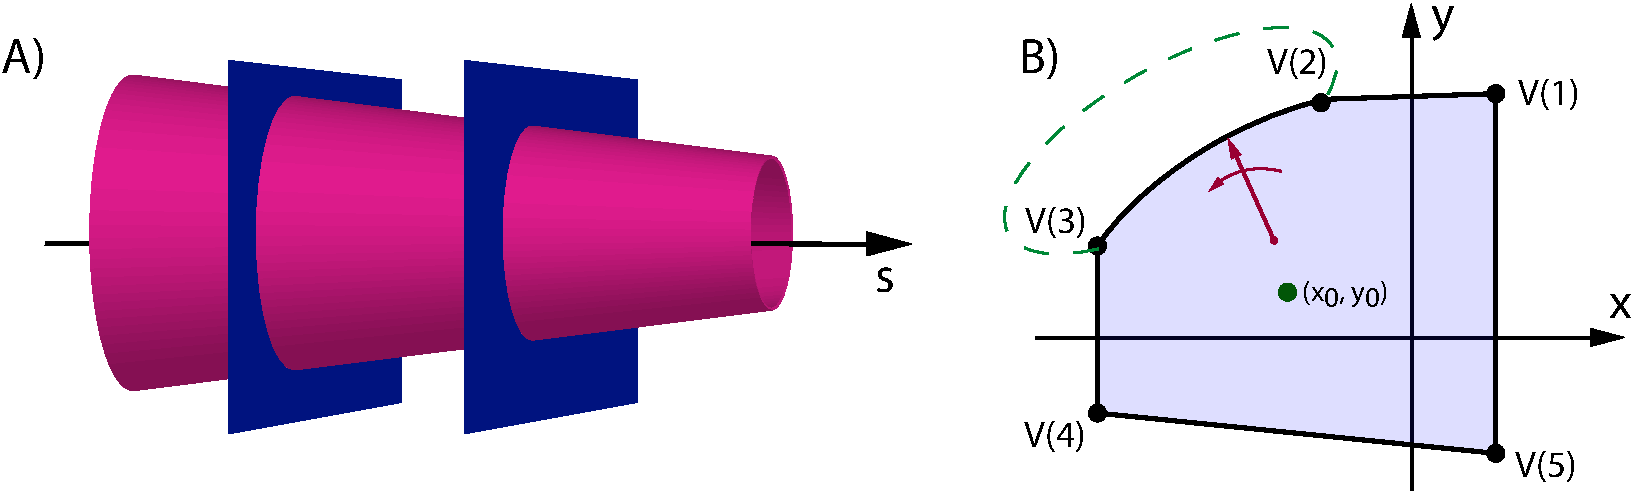
\includegraphics[width=6in]{chamber-wall.pdf}
  \caption[Capillary or vacuum chamber wall.]
{A) The inside wall of a capillary or the vacuum chamber wall of a
non-capillary element is defined by a number of cross-sectional
slices.  B) Each cross-section is made up of a number of vertices. The
segments between the vertices can be either a line segment, the arc of
a circle, or a section of an ellipse.}
  \label{f:chamber.wall}
\end{figure}

%-----------------------------------------------------------------
\section{Chamber and Capillary Wall}
\label{s:wall}

The vacuum chamber wall shape may be defined for an element using the
\vn{wall} attribute as detailed below. For X-ray capillary elements
(\sref{s:capillary}), this construct is used to define the inside wall
of the capillary. Additionally, the \vn{diffraction_plate}
(\sref{s:diff.plate}) element uses a wall construct to define the
geometry of the clear areas on the plate.

The wall is defined by a number of cross-sectional slices as shown in
\fig{f:chamber.wall}A. Each cross-section is defined by a number of
vertices. The verticies are defined with respect to the local sector
origin $(x_0, y_0)$. The arc between each vertex may be either a
straight line, an arc of a circle, or a section of an ellipse. For a
capillary it is mandatory that a cross-section be convex. That is,
given any two points within the cross-section, all points on the line
segment connecting them must be within the cross-section.

\index{wall}\vn{section}\index{s (capillary attribute)}\index{v (capillary attribute)}
\index{dr_ds1}\index{dr_ds1}\index{n_slice_spline}
The \vn{wall} structure defines the capillary wall. The
syntax of the wall structure is:
\begin{example}
  wall = \{
    superimpose = <T/F>,
    section = \{ 
      type = <section_type>,
      s = <longitudinal_position>, 
      x0 = <value>,
      y0 = <value>,
      dr_ds = <value>,
      v(1) = \{<x>, <y>, <radius_x>, <radius_y>, <tilt>\}, 
      v(2) = \{ ... \},
      ...\},
    section = \{
      s = <longitudinal_position>, 
      v(1) = \{... \},
      ... \},
    ... \}
\end{example}
Example:
\begin{example}
  this_cap: capillary, 
    wall = \{   
      section = \{ ! cross-section with top/bottom symmetry
        s = 0, v(1) =  \{0.02, 0.00\}, 
        v(2) = \{0.00, 0.02, 0.02\}, v(3) = \{-0.01, 0.01\} \}, 
      section = \{  ! Cross-section that is a tilted ellipse.
        s = 0.34, 
        v(1) = \{0.003, -0.001, 0.015, 0.008, 0.2*pi\} \} \}
\end{example}
In this example an element called \vn{this_cap} is a \vn{capillary}
whose wall is defined by two cross-sections.

The wall structure begins with ``\vn{wall = \{}'' and ends with a
``\vn{\}}''. In between are a number of individual cross-section
structures. Each individual cross-section begins with ``\vn{section =
\{}'' and ends with a ``\vn{\}}''. The \vn{s} parameter of a
cross-section gives the longitudinal position of the cross-section.

For a capillary, \vn{s} must be zero for the first cross-section and
the length of the capillary is given by the value of \vn{s} of the
last cross-section.

The \vn{v(<j>)} within a cross-section define the vertices for each
cross-section. The vertices are defined with respect to the section
origin given by \vn{x0} and \vn{y0}. Each \vn{v(<j>)} has five
parameters. It is mandatory to specify the first two parameters
\vn{<x>} and \vn{<y>}. Specifying the rest, \vn{<radius_x>},
\vn{<radius_y>}, and \vn{<tilt>}, is optional. The default values, if
not specified, is zero. The point (\vn{<x>}, \vn{<y>}) defines the
position of the vertex. The parameters \vn{<radius_x>},
\vn{<radius_y>}, and \vn{<tilt>} define the shape of the segment of
the cross-section between the given vertex and the preceding one.
\begin{example}
  <radius_x>  = 0, <radius_y>  = 0   --> Straight line segment.
  <radius_x> != 0, <radius_y>  = 0   --> Circular arc with radius = radius_x
  <radius_x>  = 0, <radius_y> != 0   --> Illegal!
  <radius_x> != 0, <radius_y> != 0   --> Ellipse section.
\end{example}
When an ellipse is specified, \vn{<radius_x>}, and \vn{<radius_y>} are
the half width and half height of the semi-major axes and the
\vn{<tilt>} parameter gives the tilt of the ellipse. \vn{<radius_x>}
and \vn{<radius_y>} must not be negative.

In the example above, for the first cross-section, \vn{v(2)}
specifies a non-zero \vn{<radius_x>} and, by default, \vn{<radius_y>}
is zero. Thus the segment of the cross-section between \vn{v(1)} and
\vn{v(2)} is circular in nature with a radius of 0.02. Since \vn{v(3)}
does not specify \vn{<radius_x>} nor \vn{<radius_y>}, the
cross-section between \vn{v(2)} and \vn{v(3)} is a straight line
segment.

The vertex points must be arranged in a ``counter clockwise manner''. 
For vertices \vn{<v(i)>} and \vn{<v(i+1)>} connected by a line segment
this translates to
\Begineq
  0 < \theta_{i+1} - \theta_{i} \pmod{2\pi} < \pi
\Endeq
where $(r_n, \theta_n)$ are the polar coordinates of the $n^{th}$
vertex. For vertices connected by an arc, ``counter clockwise manner''
means that the line segment with one end at the center of the arc and
the other end traversing the arc from \vn{<v(i)>} to \vn{<v(i+1)>}
rotates in counter clockwise as shown in
\fig{f:chamber.wall}B. 

The red line segment with one end at the center of the arc and the
other end traversing the arc from, in this case, $V(2)$ to $V(3)$,
rotates in counter clockwise manner. In general, there are two
solutions for constructing such an arc. For positive radii, the
solution chosen is the one whose center is closest to the section
origin $(x_0, y_0)$. If the radii are negative, the center point will
be the point farthest from the origin (the dashed line between $V(2)$
and $V(3)$ in the figure).

A restriction on cross-sections is that the section origin $(x_0,
y_0)$ must be in the interior of any cross-section and that for any
cross-section a line drawn from the origin at any given angle $\theta$
will intersect the cross-section at exactly one point as shown in
\fig{f:chamber.wall}B. This is an important point in the construction
of the wall between cross-sections as explained below.

The last vertex specified, call it \vn{<v(n)>}, should not have the
same \vn{<x>}, \vn{<y>} values as the first vertex \vn{<v(1)>}. That
is, there will be a segment of the cross-section connecting
\vn{<v(n)>} to \vn{<v(1)>}. The geometry of this segment is determined
by the parameters of \vn{<v(1)>}.

If there is mirror symmetry about the $x$ or $y$ axis for a
cross-section, the ``mirrored'' vertices, on the ``negative'' side of
the mirror plane, do not have to be specified. Thus if all the vertex
points of a cross-section are in the first quadrant, that is, all
\vn{<x>} and \vn{<y>} are zero or positive, mirror symmetry about both the
$x$ and $y$ axes is assumed. If all the \vn{<y>} values are zero or
positive and some \vn{<x>} values are positive and some are negative,
mirror symmetry about the $x$ axis is assumed. Finally, if all the
\vn{<x>} values are zero or positive but some \vn{<y>} values are
positive and some are negative, symmetry about the $y$ axis is
assumed. For example, for the first in the above example, since
all the \vn{<y>} values are non-negative and there are positive and
negative \vn{<x>} values, symmetry about the $x$ axis is assumed.

The one exception to the above rule that (\vn{<x>}, \vn{<y>}) is the
vertex center is when a single vertex \vn{v(1)} is specified for a
cross-section with a non-zero \vn{<radius_x>}. In this case,
(\vn{<x>}, \vn{<y>}) are taken to be the center of the circle or
ellipse. In the example above, the second cross-section is a
tilted ellipse with center at $(0.003, -0.001)$. If a cross-section
has a single vertex and \vn{<radius_x>} is
not specified, the cross-section is a rectangle. For example
\begin{example}
    section = \{ s = 0.34, v(1) = \{0.03, 0.01\} \}
\end{example}

\begin{figure}[tb]
  \centering
  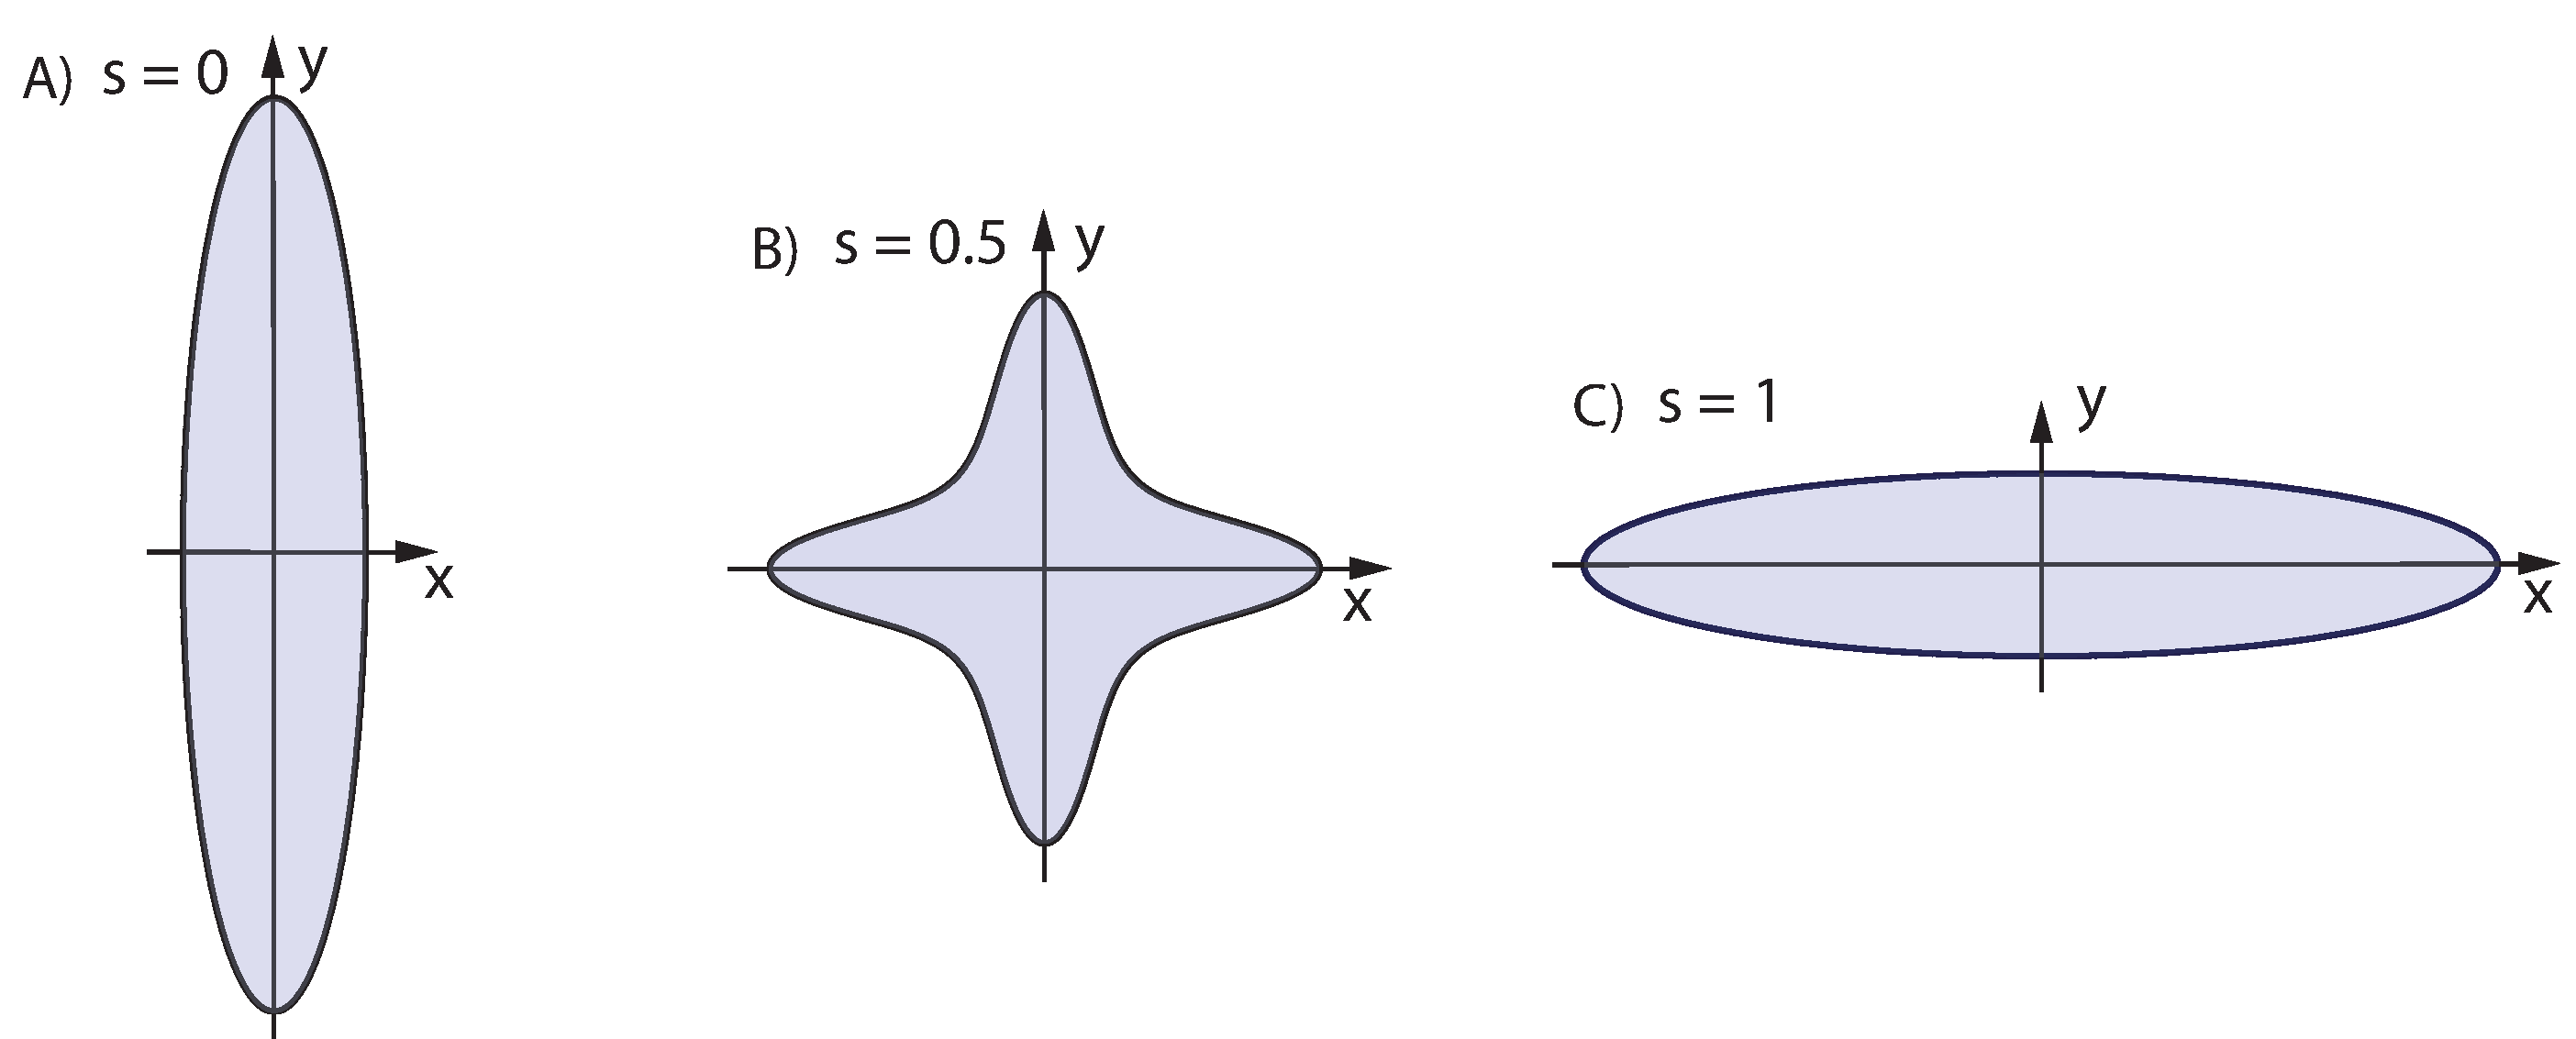
\includegraphics[width=4in]{concave-capillary.pdf}
  \caption[Convex cross-sections do not guarantee a convex volume.]
{Example where convex cross-sections do not produce a convex volume.
Cross-sections (A) and (C) are ellipses with a 5 to 1 aspect ratio.
Half way in between, linear interpolation produces a convex cross-section
as shown in (B).} 
  \label{f:concave.capillary}
\end{figure}

Between cross-sections, the wall is defined by interpolation. Let
$r_{c1}(\theta)$ be the radius of the wall as a function of $\theta$
for a given cross-section defined at $s = s_1$. Let $r_{c2}(\theta)$
be the radius function at the next defined cross-section at $s =
s_2$. The wall $r_c(\theta, s)$ at any point $s$ between $s_1$ and
$s_2$ is defined by the equation
\Begineq
  r_c(\theta, s) = p_1(\stilde) \, r_{c1}(\theta) + p_2(\stilde) \, r_{c2}(\theta)
\Endeq
where 
\Begineq
  \stilde \equiv \frac{s - s_1}{s_2 - s_1}
\Endeq
and $p_1$ and $p_2$ are cubic polynomials parameterized by
\begin{align}
  p_1 &= 1 - \stilde + a_1 \, \stilde + a_2 \, \stilde^2 + a_3 \, \stilde^3 \CRNO
  p_2 &= \stilde + b_1 \, \stilde + b_2 \, \stilde^2 + b_3 \, \stilde^3 
\end{align}
If $a_i = b_i = 0$ for all $i = 1, 2, 3$, the interpolation is linear
and this is the default if either of the parameters \vn{dr_ds1} and
\vn{dr_ds2} are not given in the wall definition. These parameters are
the slopes of the wall with respect to $s$ at the end points
\begin{equation}
  \mbox{dr_ds1} \equiv \left. \frac{d\overline{r}}{ds} \right|_{s = s_1} \comma \qquad
  \mbox{dr_ds2} \equiv \left. \frac{d\overline{r}}{ds} \right|_{s = s_2} 
\end{equation}
where $\overline{r}$ is the average $r$ averaged over all
$\theta$. When {\em both} \vn{dr_ds1} and \vn{dr_ds2} are specified, the $a_i$
and $b_i$ are calculated so that the slopes of the wall match 
the values of \vn{dr_ds1} and \vn{dr_ds2} along with the constraints.
\begin{align}
  p_1(0) &= 1 \comma \qquad p_1(1) = 0 \CRNO
  p_2(0) &= 0 \comma \qquad p_2(1) = 1 \\
  M &\equiv a_1^2 + a_2^2 + a_3^2 + b_1^2 + b_2^2 + b_3^2 \mbox{ is a minimum}
  \nonumber
\end{align}
The last constraint ensures a ``smooth'' transition between the two cross-sections.

For a capillary, in order for \bmad to quickly track photons,
\bmad assumes that the volume between the cross-sections is
convex. The volume will be convex if each cross-section $r_c(\theta,
s)$ at any given $s$ is convex. Note that it is {\em not} sufficient
for $r_c(\theta, s)$ to be convex at the specified cross-sections as
shown in \fig{f:concave.capillary}. Also note that it is perfectly
fine for the total capillary volume to not be convex.

To refer to a cross-section parameters after an element has been
defined, the following syntax is used:
\begin{example}
  ele_name[wall.section(n).v(j).x]   ! x value of j^th vertex of n^th cross-section
\end{example}

%-----------------------------------------------------------------
\subsection{Vacuum Chamber Wall}
\label{s:chamber}

The vacuum chamber wall is independent of the element apertures
(\sref{s:limit}. Unless a program is specifically constructed, the
presence of a vacuum chamber wall will not affect particle tracking.

The vacuum chamber wall defined for an element may be shorter or
longer than the element.  The vacuum chamber wall for a particular
lattice branch is the sum of all the chamber walls of the individual
elements. That is, the chamber wall at any given point is determined
by interpolation of the nearest sections upstream and downstream to
the point.  Thus a given lattice element need not contain a \vn{wall}
component for the chamber wall to be well defined at the element.

The chamber walls of any two elements may not overlap. The exception
is when the \vn{superimpose} attribute for a wall of an element is set
to True. In this case, any other wall cross-sections from any other
elements that overlap the superimposed wall are discarded.

If a branch has a closed geometry (\sref{s:param}), wall sections that
extend beyound the ends of the branch are ``wrapped'' around.

The chamber wall is defined with respect to the local coordinate
system (\sref{s:ref}). That is, in a bend a wall that has a constant
cross section is a section of a torus.

\index{patch!and chamber wall}
\vn{Patch} elements complicate the wall geometry since the coordinate
system at the end of the \vn{patch} may be arbitrarily located
relative to the beginning of the patch. To avoid confusion as to what
coordinate system a wall section belongs to, \vn{patch} elements are
not allowed to define a wall. The wall through a patch is determined
by the closest wall sections of neighboring elements. These wall
sections need to be placed at the edge of the \vn{patch}.

%-----------------------------------------------------------------

\begin{figure}[tb]
  \centering
  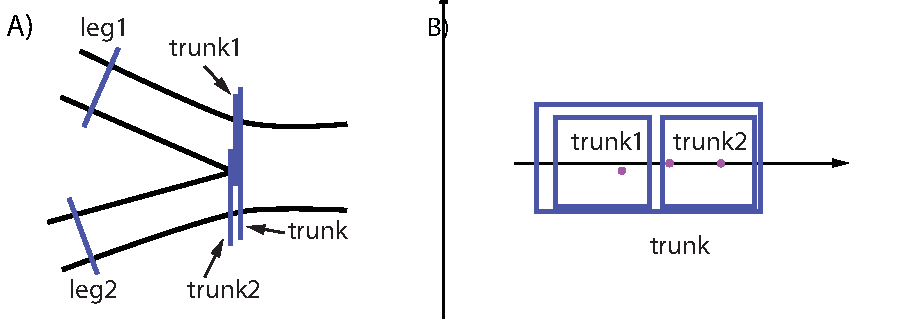
\includegraphics[width=6in]{crotch.pdf}
  \caption[vacuum chamber crotch geometry.]
{A) Crotch geometry: Two pipes labeled ``leg1'' and ``leg2'' merge
into a single pipe called the ``trunk'' pipe. Five wall sections are
used to define the crotch geometry (solid lines). Dashed lines
represent sections not involved in defining the crotch. For purposes
of illustration the three trunk sections are displaced longitudinally
but in reality must have the same longitudinal coordinate.  B) Example
layout of the crotch1, crotch2 and crotch wall sections. $O_1$, $O_2$
and $O$ are the $x_0, y_0$ origins of the sections.}
  \label{f:crotch}
\end{figure}

\index{crotch chamber geometry}
Each section has a \vn{type} attribute. This attribute is not used for 
\vn{capillary} elements. For a vacuum chamber wall, the \vn{type} 
attribute is used to dscribe a ``crotch'' geometry where
two pipes merge into one pipe. The possible values for the \vn{type} 
attribute are:
\begin{example}
  normal     ! default
  leg1
  leg2
  trunk1
  trunk2
  trunk
\end{example}
The geometry of a crotch is shown in \fig{f:crotch}A. Two pipes,
called ``leg1'' and ``leg2'', merge into one pipe called the ``trunk''
pipe.  The trunk pipe can be either upstream or downstream of the leg
pipes.  To describe this situation, five sections are needed: One
section in each leg pipe which need to have their \vn{type} attribute
set to \vn{leg1} and \vn{leg2}, and three sections in the trunk with
one having a a \vn{type} attribute of \vn{trunk1}, another having a
\vn{type} attribute of \vn{trunk2} and the third haveing a \vn{type}
attribute of \vn{trunk}. There can be no sections between the leg
sections and the trunk sections.

All three trunk sections must be associated with the same element and
have the same \vn{s} value. In the list of sections of the element
containing the trunk elements, the \vn{trunk1} and \vn{trunk2}
sections must be listed first if the leg pipes are upstream of the
trunk pipe (the situation shown in the figure) and must be listed last
if the leg pipes are downstream. That is, the \vn{trunk1} and
\vn{trunk2} sections are ``between'' the leg sections and the
\vn{trunk} section. It does not matter if \vn{trunk1} is before or
after \vn{trunk2}.

The \vn{trunk1} and \vn{trunk2} sections must not overlap and the
\vn{trunk} section must be constructed so that its area is the union
of the areas of \vn{trunk1} and \vn{trunk2}. An example is illustrated
in \fig{f:crotch}B. Here the \vn{trunk1} and \vn{trunk2} sections are
squares with origins labeled $O_1$ and $O_2$ in the figure. By
necessity, these origins must be different since each must lie within
the boundaries of their respective areas. The \vn{trunk} section is a
rectagle encomposing the two squares and has an origin labeled $O$.

Between \vn{leg1} and \vn{trunk1} sections the wall is interpolated
using these two section. Similarly for the region between \vn{leg2}
and \vn{trunk2} sections. Away from these regions interpolation is
done as outlined above but these regions need a different
interpolation scheme since, \vn{leg1} and \vn{trunk1}, as well as
\vn{leg2} and \vn{trunk2} sections do not have to be parallel to each
other.

%-----------------------------------------------------------------
\section{Length Attributes}
\label{s:l}

\index{length of elements}
\index{l|hyperbf}
\index{l_chord|hyperbf}
\index{rbend}
\index{sbend}
The length attributes are
\begin{example}
  l       = <Real>  ! 
  l_chord = <Real>  ! Chord length of a bend. Dependent attribute.
\end{example}
The length \vn{l} is the path length of the reference particle. The
one exception is for an \vn{rbend}, the length \vn{l} set in the
lattice file is the chord length (\sref{s:bend}). internally, \bmad
converts all \vn{rbend}s to \vn{sbend}s and stores the chord length
under the \vn{l_chord} attribute.
Example:
\begin{example}
  q: quadrupole, l = 0.6, k1 = 0.3425
\end{example}

\index{wiggler}
Note that for \vn{wiggler}s, the length \vn{l} is not the same as the
path length for a particle with the reference energy starting on the
reference orbit. See~\sref{s:ref}.

\index{patch}
For \vn{patch} elements the \vn{l} length is, by definition, equal to
\vn{z_offset}. For \vn{patch} elements, \vn{l} is a dependent
attribute and will be automatically set to \vn{z_offset} by \bmad.

%-----------------------------------------------------------------
\section{Is_on Attribute}
\label{s:is.on}
\index{is_on|hyperbf}

The \vn{is_on} attribute
\begin{example}
  is_on = <Logical>
\end{example}
is used to turn an element off. Turning
an element off essentially converts it into a drift.
Example
\begin{example}
  q1: quad, l = 0.6, k1 = 0.95
  q1[is_on] = False
\end{example}

\index{aperture}
\index{reference orbit}
\index{reference energy}
\vn{is_on} does not affect any apertures that are set. Additionally,
\vn{is_on} does not affect the reference orbit. Therefore, turning 
off an \vn{lcavity} will not affect the reference energy.

%-----------------------------------------------------------------
\section{Multipole Attributes: An, Bn, KnL, Tn}
\label{s:multip}

\index{multipole!an, bn|hyperbf} 
\index{multipole!knl, tn|hyperbf} 
\index{ab_multipole}
\index{multipole}
\index{radius}
A \vn{multipole} (\sref{s:mult}) element specifies its multipole
components using an Amplitude (\vn{KnL}) and a tilt (\vn{Tn})
\begin{example}
  KnL = <Real>
  Tn  = <Real>  ! Default is $pi$/(2n + 2)
\end{example}
\vn{ab_Multipole} (\sref{s:ab.m}) and all other elements that
have multipole attributes specify the multipoles using normal
(\vn{Bn}) and skew (\vn{An}) components 
\begin{example}
  An = <Real>
  Bn = <Real>
\end{example}
Here \vn{n} ranges from 0
(dipole component) through 20. Example:
\begin{example}
  q1: ab_multipole, b0 = 0.12, a20 = 1e7
\end{example}

Multipole formulas for are given in \sref{s:fields}.  Note that for
\vn{multipole} and \vn{ab_multipole} (but not any other element) a
non-zero dipole component will affect the reference orbit (just like a
normal dipole will).

The \vn{Tn} tilt component without a value takes a default of $pi$/(2n
+ 2) which makes the component \vn{skew}.  Example:
\begin{example}
  m: multipole, k1l = 0.45, t1  ! Skew quadrupole
\end{example}

For everything other than a \vn{multipole} and \vn{ab_multipole}, the
multipole strength is scaled by a factor $F \, r_0^{n_\text{ref}} /
r_0^n$ (cf.~\Eq{ababf}) where $F$ is the strength of the element (for
example $F$ is $K1 \cdot L$ for a quadrupole), and $r_0$ is the
``measurement radius'' and is set by the \vn{radius} attribute. The
default value of $r_0$, if the \vn{radius} is not given, is 1.0.  This
behavior may be turned off by setting the \vn{scale_multipoles}
attribute.  Example:
\begin{example}
  q1: quadrupole, b0 = 0.12, a20 = 1e7, scale_multipoles = F
\end{example}

%-----------------------------------------------------------------
\section{Specifying Electromagnetic Fields Via Tables or Maps}
\label{s:em.fields}

\index{lcavity}\index{rfcavity}\index{em_field}\index{field}
3D Electromagnetic fields can be specified using the \vn{field}
attribute. Fields so specified can be used with, for example,
\vn{runge_kutta} tracking (\sref{s:tkm}), etc. The \vn{field}
attribute can be used with both RF and DC fields however RF fields can
only be associated with \vn{lcavity}, \vn{rfcavity}, and \vn{em_field}
elements.

The syntax for specifying the electromagnetic fields is
\index{m}\index{field}\index{mode}\index{freq}\index{dphi0_ref}
\index{f_damp}\index{field_scale}\index{master_scale}\index{phi0_azimuth}
\index{map}\index{grid}
\begin{example}
  field = \{
    mode = \{
      m             = <Integer>, ! Mode number
      harmonic      = <Integer>, ! Harmonic number 
      dphi0_ref     = <Real>,    ! Phase of oscillations.
      f_damp        = <Real>,    ! Oscillation damping factor. Default = 0.
      field_scale   = <Real>,    ! Scale factor for the E & B fields.
      master_scale  = <Name>,    ! Master scaling parameter for E & B fields.
      phi0_azimuth  = <Real>,    ! Azimuthal orientation.
      map           = <EM_field_map>,        ! EM field map data
      grid          = \{<EM_field_grid>\} \},    ! EM field grid data
    mode = \{...\}\}
\end{example}
The electromagnetic field is specified as a series of \vn{modes}. Each
\vn{mode} has a \vn{harmonic} number which, if non-zero, identifies it
as an RF field. The field associated with a mode can be specified
using a \vn{grid} of data points or by a \vn{map} which specify the
coefficients of an analytical form for the field.

The field is scaled by two values specified by \vn{field_scale} and
\vn{master_scale}. That is
\begin{equation}
  [E, B] (actual) = [E, B] (from map or grid) * field_scale * master_scale_value
\end{equation}
That is, the actual field is the value as determined from the \vn{map}
or \vn{grid} data (see below) scaled by the value of \vn{field_scale}
times the ``master_scale_value''. This master_scale_value is the value
of the element parameter given by \vn{master_scale}. For example, for
a quadrupole element, if \vn{master_scale} is set to "K1" then the
fields are scaled by the quadrupole strength parameter. The purpose of
this \vn{master_scale} is to provide a way to scale the 3D fields with
the element strength parameter (K1 for a quadrupole) and also provide
a way to scale separate \vn{mode}s jointly.

The \vn{map} specification has the form
\begin{example}
  map = \{
    dz        = <Real>,    ! Distance between sampled field points.
    e_coef_re = (<Real>, <Real>, ....),  ! Real part of e.
    e_coef_im = (<Real>, <Real>, ....),  ! Imaginary part of e.
    b_coef_re = (<Real>, <Real>, ....),  ! Real part of b.
    b_coef_im = (<Real>, <Real>, ....),  ! Imaginary part of b.
  \}
\end{example}
For rf fields the basic equations used for the mode decomposition of
the rf fields are given in Section~\sref{s:rf.fields.phys}. 
\vn{e_re} and \vn{e_im} give the real an imaginary part of $e$ and
\vn{b_re} and \vn{b_im} give the real and imaginary part of $b$. All
of these vectors must be present and have the same length. The
exception is with an $m = 0$ mode either the $e$ or $b$ arrays can be
omitted and will default to zero. The number of terms $N$ for the $e$
or $b$ vectors must be a power of $2$ and all modes must have the same
number of terms. The $n$\Th element in the $e$ or $b$ arrays, with $n$
running from 0 to $N-1$, is associated with a wavelength $k_n$
\begin{equation}
  k_n = \begin{cases}
    \frac{2 \, \pi \, n}{N \, dz} & n < \frac{N}{2} \\
    \frac{2 \, \pi \, (n-N)}{N \, dz} & \mbox{otherwise}
  \end{cases}
\end{equation}
This convention follows the convention used by Numerical
Recipes\cite{b:nr}.  

The longitudinal length
of the field is
\begin{equation}
  L_{\mbox{field}} = \frac{N - 1}{dz}
\end{equation}
this may be different from the length \vn{l} specified for the
element. If there is a difference, the field is assumed to be centered
on the element and drifts will be used at the entrance and exit ends
of the element to make up the difference.

Alternatively, a grid of field points may be specified. The general format is:
\begin{example}
  grid = \{ 
    type = <String>,
    r0   = (<Real>, <Real>, <Real>),  ! Grid origin 
    dr   = (<Real>, <Real>, <Real>),  ! Grid spacing
    ele_anchor_pt = <Position>        ! BEGINNING, CENTER, or END
    pt(<Integer>, <Integer>, <Integer>) = ( (<Real>, <Real>), \ldots ),  ! Grid field points
    \ldots \}
\end{example}
Currently the only available value for the grid \vn{type} is 
\begin{example} 
  rotationally_symmetric_rz
\end{example} 
The format for this type of grid is 
\begin{example}
  grid = \{ 
    type = rotationally_symmetric_rz,
    r0   = (<r(0,0)>,  <z(0,0)>),     ! Grid origin 
    dr   = (<delta_r>, <delta_z>),    ! Grid spacing
    pt(i_r, i_z) = ((<Re(E_r)>, <Im(E_r)), (<Re(E_phi)>, <Im(E_phi)>), 
                                             (<Re(E_z)>, <Im(E_z)>))
    \ldots \}
\end{example}

The field of a given mode oscillates as given by Eq.~\ref{eseei}  
\Begineq
  e^{-i \, 2 \, \pi ( f \, t + \theta_0)}
\Endeq
The phase of the oscillation, $\theta_0$ comes from two
sources: the phase \vn{dphi0_ref} set for the mode and an overall phase
\vn{phi_ref} given by
\begin{example}
 phi_ref = phi0 + dphi0
\end{example}
\index{lcavity!reference phase}\index{rfcavity!reference phase}
Unfortunately, to be consistent with \mad, the definition of
\vn{phi_ref} for an \vn{lcavity} (\sref{s:lcav}) differs in sign to
that for an \vn{rfcavity} (\sref{s:rfcav}). This being the case,
$\theta_0$ is
\Begineq
  \theta_0 = 
  \begin{cases}
    \mbox{dphi0_ref} + \dsfrac{f}{f_0} \, (\mbox{phi_ref} + \mbox{phi0_err}) & 
    \mbox{lcavity element} \\
    \mbox{dphi0_ref} - \dsfrac{f}{f_0} \, \mbox{phi_ref} & 
    \mbox{rfcavity element}
  \end{cases}
\Endeq
where $f$ is the mode frequency and $f_0$ is the frequency of the fundamental.

The phase \vn{dphi0_ref} of the fundamental mode is auto-scaled by Bmad
so that a particle with $z = 0$ will go through the cavity on crest
for a \vn{lcavity} and on the zero-crossing for an
\vn{rfcavity}. Additionally, the field of the fundamental mode is
adjusted by an overall factor so that for an \vn{lcavity} the maximal
acceleration is equal to \vn{gradient * L} and for an \vn{rfcavity}
the maximal acceleration is equal to \vn{e * voltage}.

%-----------------------------------------------------------------
\section{RF Couplers}
\label{s:rf.coupler}

\index{lcavity}\index{rfcavity}
\index{coupler_at}\index{coupler_strength}
\index{coupler_angle}\index{coupler_phase}
For \vn{lcavity} and \vn{rfcavity} elements, the attributes that
characterize the dipole transverse kick due to a coupler port are:
\begin{example}
  coupler_at       = <Switch> ! What end the coupler is at
  coupler_strength = <Real>   ! Normalized strength
  coupler_angle    = <Real>   ! Polarization angle (rad/2\(\pi\))
  coupler_phase    = <Real>   ! Phase angle with respect to the RF (rad/2\(\pi\))
\end{example}
The possible \vn{coupler_at} settings are:
\begin{example}
  entrance_end
  exit_end  ! default
  both_ends
\end{example}
The kick due to the coupler is
\begin{example}
  dP_x = amp * cos(phase) * cos(angle) 
  dP_y = amp * cos(phase) * sin(angle)
  dE   = amp * (cos(angle) * x + sin(angle) * y) * sin(phase) * twopi * rf_frequency / c_light 
\end{example}
where \vn{dP_x} and \vn{dP_y} are the transverse momentum kicks, \vn{dE} is an energy kick, and
\begin{example}
  amp   = gradient * coupler_strength 
  phase = twopi * (phi_particle + phi_ref + coupler_phase)         ! For lcavity \sref{s:lcav}
        = pi/2 + twopi * (phi_particle - phi_ref + coupler_phase)  ! For rfcavity \sref{s:lcav}
  angle = twopi * coupler_angle
\end{example}
The energy kick is needed to keep things symplectic. 

Example:
\begin{example}
  rf1: lcav, l = 4.5, gradient = 1.2e6, coupler_at = both_ends, rf
                                                  coupler_strength = 0.037
\end{example}

%-----------------------------------------------------------------
\section{RF Wakes}
\label{s:rf.wakes}

Wake fields can be specified for \vn{lcavity} and \vn{rfcavity} elements.
The attributes that characterize the wakes are:
\index{sr_wake_file}\index{lr_wake_file}\index{lr_freq_spread}
\begin{example}
  sr_wake_file     = <String> ! Short range wake field definition file.
  lr_wake_file     = <String> ! Long range wake field definition file.
  lr_freq_spread   = <Real>   ! Frequency spread of the LR wake fields.
\end{example}

The formulas used to compute the wake field are given in
\sref{s:wake.fields}.  The input file name for the short--range
wake fields is specified using the \vn{sr_wake_file} attribute. The
file gives both monopole longitudinal and dipole transverse
wakes. Comment lines may be included by starting a line with an
exclamation mark (!). Blank lines are also ignored.  An example input
file is:
\begin{example}
  !    z           Wz             Wt
  !   [m]       [V/C/m]       [V/C/m^2]
   0.000E+00  1.61125E+15   0.00000E+00     1 
  -1.000E-05  1.44516E+15  -1.30560E+15     2 
  -2.000E-05  1.38148E+15  -2.50665E+15     3 
  .. etc ..
  -1.970E-03  3.49958E+14  -7.95507E+16   198 
  -1.980E-03  3.48606E+14  -7.97253E+16   199  
  -1.990E-03  3.47263E+14  -7.98989E+16   200
     END_SECTION


  ! Pseudo Wake modes:
  !                      Amp       damp          k      phase
  ! Longitudinal:      [V/C/m]     [1/m]      [1/m]     [rad]  
  ! Transverse:      [V/C/m^2]     [1/m]      [1/m]     [rad]  

  &short_range_modes
    longitudinal(1) = 3.23e14     1.23e3     3.62e3     0.123
    longitudinal(2) = 6.95e13     5.02e2     1.90e3    -1.503
    .. etc ..
    transverse(1) =   4.23e14     2.23e3     5.62e3     0.789
    transverse(2) =   8.40e13     5.94e2     1.92e3     1.455
     .. etc ..
    z_max = -1.3e-3
  /
\end{example}
The file is divided into two sections with a line containing the word
\vn{END_SECTION} marking the division between the sections.  Wakes can
be specified via a table of wake versus longitudinal position $z$
and/or using a set of ``pseudo'' modes (\sref{s:wake.fields}). The
first section gives the wake vs $z$ table, and the second section
gives the longitudinal monopole and transverse dipole pseudo modes.
The range of the table is from $0$ to $z_{cut}$ where $z_{cut}$ is the
$z$ value in the last line of the table. If the longitudinal distance
$dz$ between two particles is within the range of the table then the
table will be used to calculate the wake kick for this pair. If $dz$
is larger than $z_{cut}$ the pseudo modes will be used. The pseudo
modes are valid from $z_{cut}$ to \vn{z_max}. 

In the first section with the table of wake vs. $z$, the first column is the
longitudinal distance $z$. $z$ must start at 0 and must increment by the a
constant amount from row to row. $z$ is negative since the wake extends behind
a particle. The second column is the longitudinal wake function in $V/C/m$. The
third column is the transverse wake in $V/C/m^2$. Any additional columns are
ignored.  Wake field formulas are to be found in \sref{s:wake.fields}.  The
wake field file is only used with macroparticle and particle distribution
tracking.  When the short--range wake field file is used with either of these
the \vn{e_loss} attribute is ignored. However, even in this case, a finite
\vn{e_loss} value will affect the reference energy. Since the quantities like
quadrupole k1 strengths and bend strengths are referenced to the reference
energy, The value of \vn{e_loss} will affect the results even with a
short--range wake field file.

The input file name for the long--range wake fields is specified using
the \vn{lr_wake_file} attribute. The file gives the
wake modes by specifying the frequency (in Hz), R/Q (in
$\Omega$/meter$^{2m}$), Q, and m (order number), and optionally the
polarization angle (in radians/2pi) for each cavity mode. The input
uses Fortran90 namelist syntax: The data begins with the string
\vn{\&long_range_modes} and ends with a \vn{/}. Everything outside is
ignored. Each mode is labeled \vn{lr(i)} where \vn{i} is the mode
index. An example input file is:
\begin{example}
              Freq      R/Q      Q    m   Polar   b_sin  b_cos a_sin  a_cos  t_ref 
                      [Ohm/               Angle 
              [Hz]     m^(2m)]           [Rad/2pi]
  &long_range_modes
    lr(1) = 1.650e9    0.76    7.0e4  1    unpol
    lr(2) = 1.699e9   11.21    5.0e4  1    0.15
    lr(3) =    0       0.57    1.1e6  0    unpol
  /
\end{example}
A frequency of zero is used to designate wakes that are part of the
fundamental accelerating mode. \bmad needs to know if a wake is part
of the fundamental mode due to timing issues as discussed in \sref{s:rf.time}.

If the polarization angle is set to ``\vn{unpolarized}''
the mode is taken to be unpolarized.

\vn{lr_freq_spread} is used to randomly spread out the long range mode
frequencies among different cavities. The spread is Gaussian in shape
with an RMS of \vn{lr_freq_spread} * $F$ where $F$ is the frequency of a
mode.  After the long--range modes have been defined they can be
referenced or redefined using the notation
\begin{example}
  lr(n)%freq      ! Frequency
  lr(n)%r_over_q  ! R/Q
  lr(n)%q         ! Q
  lr(n)%angle     ! Polarization Angle
\end{example}
Example:
\begin{example}
  lcav[lr(2)%freq] = 1.1 * lcav[lr(2)%freq] ! Raise frequency by 10\%
\end{example}

Example:
\begin{example}
  rf1: lcav, l = 4.5, gradient = 1.2e6, sr_wake_file = "sr1.dat"
\end{example}

%-----------------------------------------------------------------
\section{Fringe Fields}
\label{s:fringe}
\index{fringe fields}

\index{fringe_type}\index{kill_fringe}
The tracking through the fringe fields of such elements as bends,
quadrupoles, etc is determined by the following element attributes
\begin{example}
  fringe_type    !  
  kill_fringe
\end{example}

The \vn{kill_fringe} may be set to one of
\begin{example}
  no_end               ! Default
  both_ends
  entrance_end
  exit_end
\end{example}
The \vn{kill_fringe} switch is used for vetoing fringe effects at
either of the faces of the element. This is useful in vetoing the
fringe effect in the interior of split elements.

The \vn{fringe_type} may be set to one of the following
\begin{example}
  none              ! Default for non-bend elements.
  basic_bend        ! Default for sbend and rbend elements
  full_bend
  full_straight
\end{example}
The \vn{none} setting ignores any fringe fields and is the default for
\vn{quadrupoles}, \vn{sextupoles}, etc. The \vn{basic bend} setting,
which is the default for \vn{rbend} and \vn{sbend} elements, is
essentially the basic vertical focusing effect that is present when
there is a finite \vn{e1} or \vn{e2} face angle. With
\vn{bmad_standard} tracking, \vn{basic_bend} also includes second
order terms.  In some cases, for instance in a chicane,
\vn{basic_bend} is not good enough. With \vn{full_bend} or
\vn{full_straight}, higher order effects are taken into account.  The
difference between \vn{full_bend} and \vn{full_straight} is that with
\vn{full_bend} the fringe field is calculated assuming that there is
translational invariance along the horizontal $x$ axis (as one would have 
in a bend) and for \vn{full_straight} the fringe_field i

Example:
\begin{example}
  b1: rbend, angle = pi/4, g = 0.3, fringe_type = full_bend
\end{example}

\index{ptc_max_fringe_order}
When using PTC tracking (\sref{s:ptc.intro}), the
\vn{parameter[ptc_max_fringe_order]} (\sref{s:param}) determines the maximum
order of the calculated fringe fields.

\index{permfringe}\index{bendfringe}
For programmers who deal with PTC directly: The translation between
\vn{fringe_type} on the \bmad side and \vn{permfringe} and \vn{bendfringe} 
on the PTC side is:
\begin{center}
\begin{tabular}{lll} \hline 
{\em fringe_type} & {\em permfringe} & {\em bendfringe} \\ \hline
  none            & False            & False            \\    
  basic_bend      & False            & True             \\    
  full_bend       & True             & True             \\    
  full_straight   & True             & False            \\    
\end{tabular}
\end{center}

%-----------------------------------------------------------------
\section{Instrumental Measurement Attributes}
\label{s:meas.attrib}

\index{instrument}\index{monitor}\index{marker}
\index{x_gain_err}\index{y_gain_err}\index{crunch}\index{noise}
\index{x_gain_calib}\index{y_gain_calib}\index{crunch_calib}
\index{x_offset}\index{y_offset}\index{tilt}
\index{x_offset_calib}\index{y_offset_calib}\index{tilt_calib}
\index{de_eta_meas}\index{n_sample}\index{osc_amplitude}

\vn{instrument}, \vn{monitor}, and \vn{marker} elements have special
attributes to describe orbit, betatron phase, dispersion and coupling
measurements. These attributes are:
\hfill\break
\hspace*{0.1in}
\begin{tabular}{llll}
  {\em Attribute}     &            &! {\em Symbol} (\sref{s:meas.calc}) & \\
  \vn{tilt}           &= <Real>    &! $\theta_t$            & See \sref{s:offset} \\ 
  \vn{x_offset}       &= <Real>    &! $x_{\mss{err}}$       & See \sref{s:offset} \\ 
  \vn{y_offset}       &= <Real>    &! $y_{\mss{err}}$       & See \sref{s:offset} \\ 
  \vn{x_gain_err}     &= <Real>    &! $dg_{x,\mss{err}}$    & Horizontal gain error \\ 
  \vn{y_gain_err}     &= <Real>    &! $dg_{y,\mss{err}}$    & Vertical gain error \\ 
  \vn{crunch}         &= <Real>    &! $\psi_{\mss{err}}$    & Crunch angle \\ 
  \vn{tilt_calib}     &= <Real>    &! $\theta_{\mss{err}}$  & tilt angle calibration \\ 
  \vn{x_offset_calib} &= <Real>    &! $x_{\mss{cal}}$       & Horizontal offset calibration \\ 
  \vn{y_offset_calib} &= <Real>    &! $y_{\mss{cal}}$       & Vertical offset calibration \\ 
  \vn{x_gain_calib}   &= <Real>    &! $dg_{x,\mss{cal}}$    & Horizontal gain calibration \\ 
  \vn{y_gain_calib}   &= <Real>    &! $dg_{y,\mss{cal}}$    & Vertical gain calibration \\ 
  \vn{crunch_calib}   &= <Real>    &! $\psi_{\mss{cal}}$    & Crunch angle calibration \\ 
  \vn{noise}          &= <Real>    &! $n_f$                 & Noise factor \\ 
  \vn{de_eta_meas}    &= <Real>    &! $dE/E$                & Percent change in energy \\ 
  \vn{n_sample}       &= <Real>    &! $N_s$                 & Number of sampling points \\ 
  \vn{osc_amplitude}  &= <Real>    &! $A_{\mss{osc}}$       & Oscillation amplitude \\ 
\end{tabular}
\hfill\break
A program can use these quantities to calculate ``measured'' values from the
``laboratory'' values. Here, ``laboratory'' means as calculated from some model lattice.
See \sref{s:meas.calc} for the conversion formulas.

\chapter{Beam Lines, and Replacement Lists}
\label{c:sequence}

To \bmad a ``lattice''\index{Lattice} is the sequence of physical
elements that is to be studied. The lattice is constructed in the
input lattice file using what are know as Beam Lines and Replacement
Lists. Beam Lines are further subdivided into Lines with and without
replacement arguments. This essentially corresponds to the \MAD
definition of Lines and Lists. There can be multiple Beam Lines and
Replacement Lists defined in a lattice file and Lines and Lists can be
nested inside other Lines and Lists. The particular Line that defines
the lattice to be analyzed by \bmad is selected by the \vn{use}
statement. For example
\begin{example}
  use, my_line
\end{example}
would pick the Line \vn{my_line} for analysis. 
Note that the names of the elements in the
lattice are always converted to upper case.

%-----------------------------------------------------------------------------
\section{Beam Lines without Arguments}
\index{Line|textbf}

A Beam Line without arguments has the format
\begin{example}
  label: LINE = (member1, member2, ...)
\end{example}
where \vn{member1}, \vn{member2}, etc. are either elements, other Beam
Lines or Replacement Lists, or sublines enclosed in parentheses.
Example:
\begin{example}
  line1: line = (a, b, c)
  line2: line = (d, line1, e)
  use, line2
\end{example}
This example shows how an Line member can refer to another Beam Line.
This is helpful if the same sequence of elements appears repeatedly in
the lattice. When \vn{line2} is expanded to form the lattice the
definition of \vn{line1} will be inserted in to produce the following
lattice for analysis
\begin{example}
  (d, a, b, c, e)
\end{example}

A member that is a Line or List can be reflected 
(elements taken in reverse order) if
a negative sign is put in front of it. For example:
\begin{example}
  line1: line = (a, b, c)
  line2: line = (d, -line1, e)
\end{example}
\vn{line2} when expanded gives
\begin{example}
  (d, c, b, a, e)
\end{example}
Reflecting a subline will also reflect any sublines of the subline. For
example:
\begin{example}
  line0: line = (y, z)
  line1: line = (line0, b, c)
  line2: line = (d, -line1, e)
\end{example}
\vn{line2} when expanded gives
\begin{example}
  (d, c, b, z, y, e)
\end{example}

A repetition count, which is an integer followed by an asterisk, 
means that the member is
repeated. For example
\begin{example}
  line1: line = (a, b, c)
  line2: line = (d, 2*line1, e)
\end{example}
\vn{line2} when expanded gives
\begin{example}
  (d, a, b, c, a, b, c, e)
\end{example}
Repetition count can be combined with reflection. For example
\begin{example}
  line1: line = (a, b, c)
  line2: line = (d, -2*line1, e)
\end{example}
\vn{line2} when expanded gives
\begin{example}
  (d, c, b, a, c, b, a, e)
\end{example}
Instead of the name of a Line, subline members can also be given as an explicit 
list using parentheses. For example, the previous example could be rewritten as
\begin{example}
  line2: line = (d, -2*(a, b, c), e)
\end{example}

%-----------------------------------------------------------------------------
\section{Beam Lines with Replaceable Arguments}
\index{Line!with arguments}

Beam lines can have an argument list using the following syntax
\begin{example}
  line_name(dummy_arg1, dummy_arg2, ...): LINE = (member1, member2, ...)
\end{example}
The dummy arguments are replaced by the actual arguments when the Line is used
elsewhere. For example:
\begin{example}
  line1(DA1, DA2): line = (a, DA2, b, DA1)
  line2: line = (h, line1(y, z), g)
\end{example}
When \vn{line2} is expanded the actual arguments of \vn{line1}, in this
case \vn(y, z), replaces the dummy arguments \vn{(DA1, DA2)} to give for
\vn{line2}
\begin{example}
  (h, a, z, b, y, g)
\end{example} 
Unlike \MAD, Beam Line actual arguments can only be elements or Beam Lines. 
Thus the following is not allowed
\begin{example}
  line2: line = (h, line1(2*y, z), g)   ! NO: 2*y NOT allowed as an argument.
\end{example}

%-----------------------------------------------------------------------------
\section{Replacement Lists}
\index{List}

When a lattice is expanded, all the lattice members that correspond to a 
name of a Replacement List 
are replaced successively, by the members
in the Replacement List. The general syntax is
\begin{example}
  label: LIST = (member1, member2, ...)
\end{example}
For example:
\begin{example}
  list1: list = (a, b, c)
  line1: line = (z1, list1, z2, list1, z3, list1, z4, list1)
  use, line1
\end{example}
When the lattice is expanded the first instance of \vn{list1} in
\vn{line1} is replaced by \vn{a} (which is the first element of
\vn{list1}), the second instance of \vn{list1} is replaced by \vn{b},
etc. If there are more instances of \vn{list1} in the lattice then
members of \vn{list1}, the replacement starts at the beginning of
\vn{list1} after the last member of \vn{list1} is used. In this case the
lattice would be
\begin{example}
  (z1, a, z2, b, z3, c, z4, a)
\end{example}
Unlike \MAD members of a replacement list can only be simple elements 
without reflection or repetition count and not other Lines or Lists. 
For example the following is not allowed:
\begin{example}
  list1: list = (2*a, b)  ! NO: No repetition count allowed.
\end{example}

\chapter{Miscellaneous Statements}

This chapter deals with the statements not covered in the previous chapters.

%-----------------------------------------------------------------------------
\section{Parameter Statement}
\label{s:param}
\index{Statement!parameter}


\index{Statement!parameter!lattice}
\index{Statement!parameter!lattice_type}
\index{Statement!parameter!taylor_order}
\index{Statement!parameter!beam_energy}
\index{Statement!parameter!ran_seed}
The \vn{parameter} statement is used to set the \vn{lattice} name and other variables. 
The variables that can be set by \vn{parameter} is
\begin{example}
  parameter[lattice]      = String      ! Lattice name 
  parameter[lattice_type] = Switch      ! 
  parameter[taylor_order] = Integer     ! Default: 3
  parameter[beam_energy]  = Real        ! Total Energy. Default: 0
  parameter[ran_seed]     = Integer     ! Random number generator init.
\end{example}

\noindent
Examples
\begin{example}
  parameter[lattice]      = "L9A19C501.FD93S_4S_15KG"
  parameter[lattice_type] = circular_lattice
  parameter[taylor_order] = 5
  parameter[beam_energy]  = 5.6e9    ! eV
\end{example}

For more information on \vn{parameter[ran_seed]} see Section~\ref{s:functions}.

The \vn{parameter[beam_energy]} is the reference energy at the start of the
lattice.  Each element in a lattice has an individual reference
\vn{beam_energy} which is a dependent parameter. 
The reference energy will only change between \vn{LCavity} or
\vn{Patch} elements. The starting reference energy must always be set.

The \vn{lattice} name is stored by \bmad for use by a program but it does
not otherwise effect any \bmad routines. 
Historically it is possible to set the lattice name using the syntax
\begin{example}
  lattice = String   ! DO NOT USE THIS SYNTAX
\end{example}
This syntax is obsolete since a typographical error is not easily caught.

\noindent
Valid \vn{lattice_type} switches are
\begin{example}
  circular_lattice  ! Default w/o LCavity element present.
  linear_lattice     ! Default if LCavity elements present.
\end{example}
a \vn{circular_lattice} is for a closed ring where one expects a
periodic solution for the Twiss parameters. A \vn{linear_lattice} is
not closed so that the initial Twiss parameters need to be given, not
computed. Although \vn{circular_lattice} is the nominal default, If
there are \vn{Lcavity} elements present, \vn{linear_lattice} will be used
as the default.

The Taylor order (cf.~\ref{s:taylor_phys}) is the maximum order for a
Taylor map.  Historically it is possible to set the Taylor order using
the syntax
\begin{example}
  taylor_order = Integer   ! DO NOT USE THIS SYNTAX
\end{example}
This syntax is obsolete since a typographical error is not easily caught.

%-----------------------------------------------------------------------------
\section{Beam Statement}
\index{Statement!beam}

\index{Statement!beam!energy}
\index{Statement!beam!particle}
\index{Statement!beam!n_part}
The \vn{Beam} statement is provided for compatibility with \MAD. The syntax is
\begin{example}
  beam, energy = GeV, particle = Switch, n_part = Real
\end{example}
For example
\begin{example}
  beam, energy = 5.6  ! Note: Gev to be compatible with \MAD
  beam, particle = electron, n_part = 1.6e10
\end{example}
Setting the reference energy using the \vn{energy} attribute is the same
as using \vn{parameter [beam_energy]}. Valid \vn{particle}
switches are
\begin{example}
  positron  ! default
  electron
\end{example}

%-----------------------------------------------------------------------------
\section{Title Statement}
\index{Statement!title}

The \vn{title} statement sets a title string which can be used by a program. 
For consistency there are two possible syntaxes
\begin{example}
  title, String
\end{example}
or
\begin{example}
  title
  String
\end{example}
For example
\begin{example}
  title
  "This is a title"
\end{example}

%--------------------------------------------------------------------------
\section{Call Statement}
\index{Statement!call}

It is frequently convenient to separate the lattice definition into
several files.  Typically there might be a file (or files) that define
the layout of the lattice (something that doesn't change often) and a
file (or files) that define magnet strengths (something that changes
more often).  The \vn{call} is used to read in separated lattice
files. The syntax is
\begin{example}
  call, filename = String
\end{example}
Example:
\begin{example}
  call, filename = "../layout/my_layout.bmad"
\end{example}
\bmad will read the called file until a \vn{return} or \vn{end_file}
statement is encountered or the end of the file is reached.

The called file will be searched for in multiple directories.
The search path for files without a directory specification in their name is:
\begin{example}
	1) Current directory
	2) directory of the calling file
	3) BMAD_LAYOUT (system logical)
\end{example}
The first instance where a file is found is used.
The search path for files with a directory specification in their name
is relative to the above list. Thus, in the above example, the search
would be
\begin{example}
  1) ../layout/my_layout.bmad  (relative to the current directory)
  2) ../layout/my_layout.bmad  (relative to the calling file directory)
  3) \$BMAD_LAYOUT:../layout/my_layout.bmad 
\end{example}

%--------------------------------------------------------------------------
\section{Return and End\_File statements}
\index{Statement!return}
\index{Statement!end_file}

\vn{Return} and \vn{end_file} have identical effect and tell \bmad to
ignore anything beyond the \vn{return} or \vn{end_file} statement in
the file.

%--------------------------------------------------------------------------
\section{Beginning Statement}
\index{Statement!beginning}

\index{Statement!beginning!beta_x}
\index{Statement!beginning!alpha_x}
\index{Statement!beginning!phi_x}
\index{Statement!beginning!eta_x}
\index{Statement!beginning!etap_x}
\index{Statement!beginning!beta_y}
\index{Statement!beginning!alpha_y}
\index{Statement!beginning!phi_y}
\index{Statement!beginning!eta_y}
\index{Statement!beginning!etap_y}
\index{Statement!beginning!cij}
\index{Statement!beginning!beam_energy}
For non--circular lattices the \vn{beginning} statement can be used to
set the Twiss parameters and beam energy at the beginning of the ring
\begin{example}
  beginning[beta_x]  = Real  ! "a" mode beta
  beginning[alpha_x] = Real  ! "a" mode alpha
  beginning[phi_x]   = Real  ! "a" mode phase
  beginning[eta_x]   = Real  ! "a" mode dispersion
  beginning[etap_x]  = Real  ! "a" mode dispersion derivative.
  beginning[beta_y]  = Real  ! "b" mode beta
  beginning[alpha_y] = Real  ! "b" mode alpha
  beginning[phi_y]   = Real  ! "b" mode phase
  beginning[eta_y]   = Real  ! "b" mode dispersion
  beginning[etap_y]  = Real  ! "b" mode dispersion derivative.
  beginning[cij]     = Real  ! C coupling matrix. i, j = {``1'', or ``2''} 
  beginning[beam_energy] = Real  ! Total energy in eV.
\end{example}
\index{Statement!parameter!beam_energy}
The \vn{gamma_x}, \vn{gamma_y}, and \vn{gamma_c} (the coupling gamma factor) 
will be kept consistent with the values set. If not set the default values are all zero. 
\vn{beginning[energy]} and \vn{parameter[beam_energy]} are equivalent and one or the other
may be set but not both.

\index{Statement!beginning!x_position}
\index{Statement!beginning!y_position}
\index{Statement!beginning!z_position}
\index{Statement!beginning!theta_position}
\index{Statement!beginning!phi_position}
\index{Statement!beginning!psi_position}
For any lattice the \vn{beginning} statement can be used to set the starting floor position 
(see~\ref{s:global}). The syntax is
\begin{example}
  beginning[x_position]     = Real  ! X position
  beginning[y_position]     = Real  ! Y position
  beginning[z_position]     = Real  ! Z position
  beginning[theta_position] = Real  ! Angle on floor
  beginning[phi_position]   = Real  ! Angle of attack
  beginning[psi_position]   = Real  ! Roll angle
\end{example}

%----------------------------------------------------------------------------
\section{Expand\_lattice Statement}
\label{s:lat_expand}
\index{Lattice!expansion|textbf}
\index{Statement!expand_lattice}

At some point in parsing a lattice file, the ordered sequence of
elements that form a lattice must be constructed. This process is
called \vn{lattice expansion} since the element sequence can be built
up from sub--sequences. Normally lattice expansion happens
automatically at the end of parsing the lattice file but an explicit
\vn{expand_lattice} statement will cause immediate expansion. The
reason why this can be important is that there are restrictions, on
some types of operations which must come either before or after
lattice expansion. 
\begin{Itemize}
\item 
\index{Intrinsic functions!ran}
\index{Intrinsic functions!ran_gauss}
The \vn{ran} and \rn{ran_gauss} functions, when used with elements
that show up multiple times in a lattice, generally need to be used
after lattice expansion. See \sref{s:functions}.
\item 
Some dependent variables may be set as if they are independent
variables but only if done before lattice expansion. See
\sref{s:depend}.
\index{Clone}
\item 
Setting \vn{dphi0} for an \vn{Lcavity} or \vn{RFcavity} clone may only
be done after lattice expansion.
\end{Itemize}

%--------------------------------------------------------------------------
\section{Debugging Statements}
\index{Statement!parser_debug}
\index{Statement!no_digested}
\index{Lattice files!parser debugging}

There are two statements, \vn{parser_debug} and \vn{no_digested},
which can help in debugging the \bmad lattice parser
itself.  That is, these statements are generally only used by programmers.

The \vn{no_digested} statement if present, will prevent \bmad from 
creating a digested file. 

The \vn{parser_debug} statement will cause information about the
lattice to be printed out at the terminal. It is recommended that this
statement be used with small test lattices since it can generate a lot
of output. The syntax is
\begin{example}
  parser\_debug \(<\)switches\(>\)
\end{example}
Valid switches are
\begin{example}
  var     ! print variable information.
  seq     ! print sequence information.
  slave   ! print full information on all regular elements.
  lord    ! print full information on all lord elements.
  lattice ! print a list of lattice element names, positions, and lengths.
  ele <n1> <n2> ...  ! print full info on selected elements.
\end{example}
Here $<n1>$, $<n2>$, etc. are the index of the selected elements in
the lattice.  Example
\begin{example}
  parser\_debug var ring ele 34 78
\end{example}





\chapter{Tracking, Spin, and Transfer Matrix Calculation Methods}
\label{c:methods}

\index{element!class}\index{tracking_method}
\index{mat6_calc_method}\index{spin_tracking_method}
\bmad allows for a number of methods that can be use to ``track'' a particle
through a lattice element. Here ``track'' can mean one of three things:
\begin{example}
  1) Calculate a particle's phase space coordinates at the exit 
     end of the element given the coordinates at the entrance end.
  2) Calculate the linear transfer map (Jacobian) through an element
     about a given reference orbit.
  3) Calculate the a particle's spin orientation at the exit end 
     of the element given the coordinates at the beginning.
\end{example}
The different tracking methods that are available have different
advantages and disadvantages in terms of speed, symplecticity, etc.
What tracking method is used, is selected on an element--by--element
basis using the attributes:
\begin{example}
  tracking_method      = <Switch>   ! phase space tracking method.
  mat6_calc_method     = <Switch>   ! 6x6 transfer matrix calculation.
  spin_tracking_method = <Switch>   ! Spin tracking method.
\end{example}
Example:
\begin{example}
  q2: quadrupole, tracking_method = boris
  q2[tracking_method] = boris
  quadrupole[tracking_method] = boris
\end{example}
The first two lines of this example have exactly the same effect in
terms of setting the \vn{tracking_method}. The third line shows how to
set the \vn{tracking_method} for an entire class of elements.

These switches are discussed in more detail in the following sections.

%----------------------------------------------------------------------------
\section{Particle Tracking Methods}
\label{s:tkm}
\index{tracking methods|hyperbf}

The \vn{tracking_method} attribute of an element sets the algorithm
that is used for single particle tracking through that element.
Table~\ref{t:track.methods} gives which methods are available for each
type of element.

A note on terminology: Adaptive step size control used with the
\vn{Runge_Kutta} integrator means that instead of taking fixed step
sizes the integrator chooses the proper step size so that the error in
the tracking is below the maximum allowable error set by \vn{rel_tol}
and \vn{abs_tol} tolerances. The advantage of step size control is
that the integrator uses a smaller step size when needed (the fields
are rapidly varying), but makes larger steps when it can. The
disadvantage is that a step is more computationally intensive since
the error in a step is estimated by repeating a step using two mini
steps. If the fields are rather uniform and you know what a good step
size is you can save time by using a fixed step size.

\begin{description}

\index{boris!tracking_method}
\item[\vn{Boris}]
Second order Boris Integration\cite{b:boris}. Like \vn{Runge_Kutta},
\vn{Boris} does tracking by integrating the equation of
motion. \vn{Boris} handles both electric and magnetic fields and does
not assume that the particle is ultra--relativistic. \vn{Boris} preserves
conserved quantities more accurately than \vn{Runge_Kutta}.

\index{bmad_standard!tracking_method}
\item[\vn{Bmad_Standard}]
Uses formulas for tracking. The formulas generally use the paraxial
approximation.  The emphasis here is on speed. Note: If an element has
non-zero multipole values, \vn{Bmad_Standard} tracking will generally
put half the multipole kick at the beginning of the element and half
at the end. This is generally a good approximation but in it can
result in differences between this and tracking methods like
\vn{Symp_Lie_PTC} which model multipoles as as distributed evenly
throughout an element.

\index{custom!tracking_method}
\item[\vn{Custom}]
This method will call a routine \vn{track1_custom} which must be
supplied by the programmer implementing the custom tracking. The
default \vn{track1_custom} supplied with the \bmad release will print
an error message and stop the program if it is called which probably
indicates a program linking problem. See \vn{s:custom.ele} for more details.

\index{linear!tracking_method}
\item[\vn{Linear}]
Linear just uses the 0th order vector with the 1st order 6x6 transfer
matrix for an element. Very simple.  Depending upon how the transfer
matrix was generated this may or may not be symplectic.

\index{MAD!tracking_method}
\item[\vn{MAD}]
This uses the MAD 2nd order transfer map. This method is not able to
handle element misalignments or kicks, and becomes inacurate as the
particle energy deviates from the reference energy. MAD tracking is
generally only used for testing purposes. Note: Thanks to CERN and
Frank Schmidt for permission to use the MAD tracking code within
\bmad.

\index{runge_kutta!tracking_method}
\item[\vn{runge_kutta}]
This uses a 4\Th order Runge Kutta integration algorithm with adaptive
step size control.  This is essentially the \vn{ODEINT} subroutine
from Numerical Recipes\cite{b:nr}. This may be slow but it should be
accurate. This method is non-symplectic. Warning: When using
\vn{custom} fields, if the fields do not obey Maxwell's equation,
there is the possibility of the \vn{runge_kutta} tracking halting mid
way through an element. See section~\sref{s:integ} for more details.

\index{symp_lie_Bmad!tracking_method}
\item[\vn{Symp_Lie_Bmad}]
Symplectic tracking using a Hamiltonian with Lie operation techniques.
This is similar to \vn{Symp_Lie_PTC} (see below) except this uses a
\bmad routine. By bypassing some of the generality inherent in PTC
(\sref{s:ptc.intro}), \vn{Symp_Lie_Bmad} achieves about a factor of 10
improvement in speed over \vn{Symp_Lie_PTC}.

\index{symp_lie_ptc!tracking_method}
\item[\vn{Symp_Lie_PTC}]
Symplectic tracking using a Hamiltonian with Lie operator techniques.
This uses Etienne Forest's PTC (\sref{s:ptc.intro}) software for the
calculation. This method is symplectic but can be slow.

\index{symp_map!tracking_method}
\item[\vn{Symp_Map}]
This uses a partially inverted, implicit Taylor map. The calculation
uses Etienne Forest's PTC software (\sref{s:ptc.intro}).  Since the map is implicit, a Newton
search method must be used. This will slow things down from the Taylor
method but this is guaranteed symplectic. Note: Due to memory limitations
in PTC, the number of elements using symp_map is limited to be of order 50.

\index{taylor!tracking_method}
\item[\vn{Taylor}]
This uses a Taylor map generated from the PTC (\sref{s:ptc.intro})
package. Generating the map may take time but once you have it it
should be very fast. One possible problem with using a Taylor map is
that you have to worry about the accuracy if you do tracking at points
that are far from the expansion point about which the map was
made. This method is non-symplectic away from the expansion
point. Whether the Taylor map is generated taking into account the
offset an element has is governed by the \vn{taylor_map_includes_offsets}
attribute (\sref{s:mapoff}). \vn{bmad_standard} and \vn{taylor}
tracking methods are identical. Note: Taylor maps for \vn{match}, and
\vn{patch} elements are limited to first order.

\index{time_runge_kutta!tracking_method}
\item[\vn{Time_Runge_Kutta}]
This method uses time as the independent variable instead of
the longitudinal $z$ position. The advantage of this method is that it can
handle particles which reverse direction longitudinally.  One use for
this method is ``dark current'' tracking where low energy particles
generated at the vacuum chamber walls can be found traveling in all
directions. Notice that \vn{time_runge_kutta} is different from using
\vn{absolute time tracking} as explained in \sref{s:rf.time}.

\end{description}

%----------------------------------------------------------------------------

\index{ab_multipole}\index{beambeam}\index{bend_sol_quad}\index{custom}
\index{drift}\index{ecollimator}\index{elseparator}\index{hkicker}
\index{instrument}\index{kicker}\index{lcavity}\index{marker}
\index{match}\index{monitor}\index{multipole}\index{octupole}
\index{patch}\index{quadrupole}\index{rbend}\index{rcollimator}
\index{rfcavity}\index{sbend}\index{sextupole}\index{solenoid}
\index{sol_quad}\index{taylor}\index{vkicker}\index{wiggler}\index{capillary}
\index{element!table of class types}
\begin{table}[pht]
\centering {
\begin{tabular}{lcccccccccccc} \toprule
\rule{0pt}{80pt} 
{\em Element Class} &
\begin{sideways}\vn{Bmad_Standard}\end{sideways} &
\begin{sideways}\vn{Boris}\end{sideways} &
\begin{sideways}\vn{Custom}\end{sideways} &
\begin{sideways}\vn{Linear}\end{sideways} &
\begin{sideways}\vn{MAD}\end{sideways} &
\begin{sideways}\vn{Runge_Kutta}\end{sideways} &
\begin{sideways}\vn{Symp_Lie_Bmad}\end{sideways} &
\begin{sideways}\vn{Symp_Lie_PTC}\end{sideways} &
\begin{sideways}\vn{Symp_Map}\end{sideways} &
\begin{sideways}\vn{Taylor}\end{sideways} &
\begin{sideways}\vn{Time_Runge_Kutta}\end{sideways} &
\\ \midrule
%                               BS   B   C   L   M   RK    SLB   SLP   SM     T   TRK
  \vn{ab_multipole}            & D &   & X & X &   &     &     &  X  &  X  &  X  &    \\  
  \vn{beambeam}                & D &   & X & X &   &     &     &     &     &     &    \\  
  \vn{bend_sol_quad}           &   &   & X &   &   &     &  D  &     &     &     &    \\  
  \vn{capillary}               & D &   & X &   &   &     &     &     &     &     &    \\  
  \vn{crystal}                 & D &   & X &   &   &     &     &     &     &     &    \\  
  \vn{custom}                  &   & X & D & X &   &  X  &     &     &     &     & X  \\  
  \vn{drift}                   & D & X & X & X & X &  X  &     &  X  &  X  &  X  & X  \\  
  \vn{e_gun}                   &   &   & X &   &   &     &     &     &     &     & D  \\  
  \vn{ecollimator}             & D & X & X & X &   &  X  &     &  X  &  X  &  X  & X  \\  
  \vn{elseparator}             & D & X & X & X & X &  X  &     &  X  &  X  &  X  & X  \\  
  \vn{em_field}                &   & X & X &   &   &  D  &     &     &     &     & X  \\  
  \vn{hkicker}                 & D & X & X & X &   &  X  &     &  X  &  X  &  X  & X  \\  
  \vn{instrument}              & D & X & X & X &   &  X  &     &  X  &  X  &  X  & X  \\  
  \vn{kicker}                  & D & X & X & X &   &  X  &     &  X  &  X  &  X  & X  \\  
  \vn{lcavity}                 & D & X & X & X &   &  X  &     &  X  &  X  &  X  & X  \\  
  \vn{marker}                  & D &   & X & X &   &     &     &  X  &  X  &  X  &    \\  
  \vn{match}                   & D &   & X &   &   &     &     &     &     &  *  &    \\ 
  \vn{monitor}                 & D & X & X & X &   &  X  &     &  X  &  X  &  X  & X  \\  
  \vn{mirror}                  & D &   & X &   &   &     &     &     &     &     &    \\  
  \vn{multipole}               & D &   & X & X &   &     &     &  X  &  X  &  X  &    \\  
  \vn{multilayer}              & D &   & X &   &   &     &     &     &     &     &    \\  
  \vn{octupole}                & D & X & X & X &   &  X  &     &  X  &  X  &  X  & X  \\ 
  \vn{patch}                   & D &   & X &   &   &  X  &     &  X  &     &  X  &    \\ 
  \vn{quadrupole}              & D & X & X & X & X &  X  &  X  &  X  &  X  &  X  & X  \\ 
  \vn{rbend}                   & D &   & X & X & X &     &     &  X  &  X  &  X  &    \\ 
  \vn{rcollimator}             & D & X & X & X &   &  X  &     &  X  &  X  &  X  & X  \\ 
  \vn{rfcavity}                & D & X & X & X & X &  X  &     &  X  &  X  &  X  & X  \\ 
  \vn{sad_mult}                & D &   & X & X &   &     &     &  X  &  X  &  X  &    \\
  \vn{sample}                  & D &   & X &   &   &     &     &     &     &     &    \\
  \vn{sbend}                   & D &   & X & X & X &  X  &     &  X  &  X  &  X  & X  \\ 
  \vn{sextupole}               & D & X & X & X & X &  X  &     &  X  &  X  &  X  & X  \\ 
  \vn{solenoid}                & D & X & X & X & X &  X  &  X  &  X  &  X  &  X  & X  \\ 
  \vn{sol_quad}                & D & X & X & X &   &  X  &  X  &  X  &  X  &  X  & X  \\ 
  \vn{taylor}                  & X &   & X & X &   &     &     &     &     &  D  &    \\ 
  \vn{vkicker}                 & D & X & X & X &   &  X  &     &  X  &  X  &  X  & X  \\ 
  \vn{wiggler} (map type)      &   & X & X & X &   &  X  &  X  &  X  &  X  &  X  & X  \\
  \vn{wiggler} (periodic type) & D & X & X & X &   &X$^a$&X$^a$&X$^a$&X$^a$&X$^a$&    \\ \bottomrule
   \multicolumn{12}{l}{$^a$See \sref{s:wiggler.periodic} for more details} \\
\end{tabular}
} 
\caption[Table of available {\bf tracking_method}\ switches for a
given element class.]{Table of available {\bf tracking_method}\
switches for a given element class. ``D'' denotes the default
method. ``X'' denotes an available method. ``*'' denotes that the
Taylor map will only be first order. 
}

\label{t:track.methods}
\end{table}

\vfill \break

%----------------------------------------------------------------------------
\section{Linear Transfer Map Methods}
\label{s:xfer}
\index{mat6_calc_method|hyperbf}

The \vn{mat6_calc_method} attribute sets how the 6x6 Jacobian transfer
matrix for a given element is computed.  Table~\ref{t:mat6.methods}
gives which methods are available for each type of element.

\index{sympliectify}
\index{taylor_map_includes_offsets}
In addition to the \vn{mat6_calc_method} switch, 
two element attributes that can affect the way the transfer matrix is
calculated are \vn{symplectify} and \vn{taylor_map_includes_offsets}. These are
discussed in sections \sref{s:symp} and \sref{s:mapoff} respectively.

For methods that do not necessarily produce a symplectic matrix the
\vn{symplectify} attribute of an element can be set to \vn{True} to
solve the problem. See \sref{s:symp.method}. 

Symplectic integration is like ordinary integration of a function f(x)
but what is integrated here is a Taylor map. Truncating the map to
0\Th order gives the particle trajectory and truncating to 1\St\
order gives the transfer matrix (Jacobian).  The order at which a
Taylor series is truncated at is set by \vn{taylor_order} (see
\sref{s:param}. Like ordinary integration there are various
formulas that one can use to do symplectic integration. In \bmad (or
more precisely in PTC (\sref{s:ptc.intro})) you can use one of 3 methods. This is
set by \vn{integrator_order}.  \vn{integrator_order} = n where $n$ is
allowed by PTC to be 2, 4, or 6. With an integration order of $n$ the
error in an integration step scales as $dz^n$ where $dz$ is step
size. The step size $dz$ is set by the length of the element and the
value of \vn{ds_step}. Remember, as in ordinary integration, higher
integration order does not necessarily imply higher accuracy.

\begin{description}

\index{bmad_standard!mat6_calc_method}
\item[\vn{Bmad_Standard}]
Uses formulas for the calculation. The formulas generally use the
paraxial approximation. The emphasis here is on speed.

\index{custom!mat6_calc_method}
\item[\vn{Custom}]
This method will call a routine \vn{make_mat6_custom} which must be
supplied by the programmer implementing the custom transfer matrix
calculation. The default \vn{make_mat6_custom} supplied with the
\bmad release will print an error message and stop the program if it
is called which probably indicates a program linking problem.
See \vn{s:custom.ele} for more details.

\index{MAD!mat6_calc_method}
\item[\vn{MAD}]
This uses the MAD 2nd transfer map. This method is not able to
handle element misalignments or kicks, and becomes inacurate as the
particle energy deviates from the reference energy. MAD tracking is
generally only used for testing purposes. Thanks must be given
to CERN and Frank Schmidt for permission to use the MAD tracking code
within \bmad.

\index{static!mat6_calc_method}
\item[\vn{Static}]
This prevents the transfer matrix from being recomputed.
Using \vn{Static} in the input file is generally not a good idea since
it prevents the matrix from being computed in the first place.
Typically \vn{Static} is used internally in a program to prevent recomputation.

\index{symp_lie_bmad!mat6_calc_method}
\item[\vn{Symp_Lie_Bmad}]
A Symplectic calculation using a Hamiltonian with Lie operator
techniques.  This is similar to \vn{Symp_Lie_PTC} (see below) except
this uses a \bmad routine. By bypassing some of the generality
inherent in PTC, \vn{Symp_Lie_Bmad} achieves about a factor
of 10 improvement in speed over \vn{Symp_Lie_PTC}. However,
\vn{Symp_Lie_Bmad} cannot generate maps above first order.

\index{symp_lie_ptc!mat6_calc_method}
\item[\vn{Symp_Lie_PTC}]
Symplectic integration using a Hamiltonian and Lie operators.
This uses the PTC (\sref{s:ptc.intro}) software for the calculation.
This method is symplectic but can be slow.

\index{symp_map!tracking_method}
\item[\vn{Symp_Map}]
This uses a partially inverted, implicit Taylor map. The calculation
uses Etienne Forest's PTC software (\sref{s:ptc.intro}).  Since the map is implicit, a Newton
search method must be used. This will slow things down from the Taylor
method but this is guaranteed symplectic. Note: Due to memory limitations
in PTC, the number of elements using symp_map is limited to be of order 50.

\index{taylor!mat6_calc_method}
\item[\vn{Taylor}]
This uses a Taylor map generated from Etienne's PTC
package. Generating the map may take time but once you have it it
should be very fast. One possible problem with using a Taylor map is
that you have to worry about the accuracy if you do a calculation at
points that are far from the expansion point about which the map was
made. This method is non-symplectic away from the expansion
point. Whether the Taylor map is generated taking into account the
offset an element has is governed by the \vn{taylor_map_includes_offsets}
attribute (\sref{s:mapoff}). \vn{bmad_standard} and \vn{taylor}
tracking methods are identical. Note: Taylor maps for \vn{match}, and
\vn{patch} elements are limited to first order.

\index{tracking!mat6_calc_method}
\item[\vn{Tracking}]
This uses the tracking method set by \vn{tracking_method} to track 6
particles around the central orbit. This method is susceptible to inaccuracies
caused by nonlinearities. Furthermore this method
is almost surely slow. While non--symplectic, the advantage of this method
is that it is directly related to any tracking results.

\end{description}

\index{ab_multipole}\index{beambeam}\index{bend_sol_quad}\index{custom}
\index{drift}\index{ecollimator}\index{elseparator}\index{hkicker}
\index{instrument}\index{kicker}\index{lcavity}\index{marker}
\index{match}\index{monitor}\index{multipole}\index{octupole}
\index{patch}\index{quadrupole}\index{rbend}\index{rcollimator}
\index{rfcavity}\index{sbend}\index{sextupole}\index{solenoid}
\index{sol_quad}\index{taylor}\index{vkicker}\index{wiggler}
\index{crystal}\index{capillary}
\begin{table}[pth]
\centering {
\begin{tabular}{lcccccccc} \toprule
\rule{0pt}{80pt} &
\begin{sideways}\vn{Bmad_Standard}\end{sideways} &
\begin{sideways}\vn{Custom}\end{sideways} &
\begin{sideways}\vn{MAD}\end{sideways} &
\begin{sideways}\vn{Static}\end{sideways} &
\begin{sideways}\vn{Symp_Lie_Bmad}\end{sideways} &
\begin{sideways}\vn{Symp_Lie_PTC}\end{sideways} &
\begin{sideways}\vn{Taylor}\end{sideways} &
\begin{sideways}\vn{Tracking}\end{sideways}
\\ \midrule
%                               BS   C   M  Stat SLB   SLP   Tlr  Trk 
  \vn{ab_multipole}            & D & X &   & X &     &  X  &  X  & X \\  
  \vn{beambeam}                & D & X &   & X &     &     &     & X \\  
  \vn{bend_sol_quad}           &   & X &   & X &  D  &     &     & X \\  
  \vn{capillary}               & D & X &   & X &     &     &     & X \\  
  \vn{crystal}                 & D & X &   & X &     &     &     & X \\  
  \vn{custom}                  &   & D &   & X &     &     &     & X \\  
  \vn{drift}                   & D & X & X & X &     &  X  &  X  & X \\  
  \vn{e_gun}                   &   & X &   & X &     &     &     & D \\  
  \vn{ecollimator}             & D & X &   & X &     &  X  &  X  & X \\  
  \vn{elseparator}             & D & X & X & X &     &  X  &  X  & X \\  
  \vn{em_field}                &   & X &   & X &     &     &     & D \\  
  \vn{hkicker}                 & D & X &   & X &     &  X  &  X  & X \\  
  \vn{instrument}              & D & X &   & X &     &  X  &  X  & X \\  
  \vn{kicker}                  & D & X &   & X &     &  X  &  X  & X \\  
  \vn{lcavity}                 & D & X &   & X &     &  X  &  X  & X \\  
  \vn{marker}                  & D & X &   & X &     &  X  &  X  & X \\  
  \vn{match}                   & D & X &   & X &     &     &     & X \\  
  \vn{mirror}                  & D & X &   & X &     &     &     & X \\  
  \vn{monitor}                 & D & X &   & X &     &  X  &  X  & X \\  
  \vn{multipole}               & D & X &   & X &     &  X  &  X  & X \\  
  \vn{multilayer_mirror}       & D & X &   & X &     &     &     & X \\  
  \vn{octupole}                & D & X &   & X &     &  X  &  X  & X \\ 
  \vn{patch}                   & D & X &   & X &     &  X  &  X  & X \\ 
  \vn{quadrupole}              & D & X & X & X &  X  &  X  &  X  & X \\ 
  \vn{rbend}                   & D & X & X & X &     &  X  &  X  & X \\ 
  \vn{rcollimator}             & D & X &   & X &     &  X  &  X  & X \\ 
  \vn{rfcavity}                & D & X & X & X &     &  X  &  X  & X \\ 
  \vn{sad_mult}                & D & X &   & X &     &  X  &  X  & X \\ 
  \vn{sample}                  & D & X &   & X &     &     &     & X \\ 
  \vn{sbend}                   & D & X & X & X &     &  X  &  X  & X \\ 
  \vn{sextupole}               & D & X & X & X &     &  X  &  X  & X \\ 
  \vn{solenoid}                & D & X & X & X &  X  &  X  &  X  & X \\ 
  \vn{sol_quad}                & D & X & X & X &  X  &  X  &  X  & X \\ 
  \vn{taylor}                  & X & X &   & X &     &     &  D  &   \\ 
  \vn{vkicker}                 & D & X &   & X &     &  X  &  X  & X \\ 
  \vn{wiggler}                 & D & X &   & X &X$^a$&X$^a$&X$^a$& X \\ \bottomrule
  \multicolumn{9}{l}{$^a$See \sref{s:wiggler.periodic} for more details} \\
\end{tabular}
}
\caption[Table of available \vn{mat6_calc_method}\ switches for a
given element class.]{Table of available \vn{mat6_calc_method}\
switches for a given element class. ``D'' denotes the default
method. ``X'' denotes an available method.}

\label{t:mat6.methods}
\end{table}

\vfill \break

%----------------------------------------------------------------------------
\section{Spin Tracking Methods}
\label{s:spin.methods}
\index{spin tracking!methods}
\index{spin_tracking_method}

The \vn{spin_tracking_method} attribute of an elements sets the
algorithm that is used for tracking a particle's spin through that
element. Table~\ref{t:spin.methods} gives which methods are available
for each type of element.

Since speed may be an issue, \bmad has an internal global parameter
called \vn{spin_tracking_on} (\sref{s:bmad.params}) that determines
whether spin is tracked or not.  Access to this parameter is
implemented on a program-by-program basis.

\begin{description}

\index{bmad_standard!spin_tracking_method}
\item[\vn{Bmad_Standard}]
Uses formulas for the calculation. The formulas generally use the
paraxial approximation. The emphasis here is on speed.

\index{custom!spin_tracking_method}
\item[\vn{Custom}]
This method will call a routine \vn{track1_spin_custom} which must be
supplied by the programmer implementing the custom spin tracking
calculation. See \vn{s:custom.ele} for more details.

\index{tracking!mat6_calc_method}
\item[\vn{Tracking}]
If \vn{tracking_method} is set to \vn{boris}, or
\vn{runge_kutta} then the spin will be tracked along with the phase
space particle coordinates using the local fields. For all other
\vn{tracking_method}s, the spin will be tracked using the
\vn{bmad_standard} spin tracking method.

\index{symp_lie_ptc!spin_tracking_method}
\item[\vn{Symp_Lie_PTC}]
Symplectic integration using a Hamiltonian and Lie operators.
This uses Etienne's PTC software for the calculation.
This method is symplectic but can be slow.

\end{description}

Example:
\begin{example}
  q: quadrupole, spin_tracking_method = symp_lie_ptc
\end{example}


\index{ab_multipole}\index{beambeam}\index{bend_sol_quad}\index{custom}
\index{drift}\index{ecollimator}\index{elseparator}\index{hkicker}
\index{instrument}\index{kicker}\index{lcavity}\index{marker}
\index{match}\index{monitor}\index{multipole}\index{octupole}
\index{patch}\index{quadrupole}\index{rbend}\index{rcollimator}
\index{rfcavity}\index{sbend}\index{sextupole}\index{solenoid}
\index{sol_quad}\index{taylor}\index{vkicker}\index{wiggler}
\index{crystal}\index{capillary}
\begin{table}[pth]
\centering {
\begin{tabular}{lcccc} \toprule
\rule{0pt}{80pt} &
\begin{sideways}\vn{Bmad_Standard}\end{sideways} &
\begin{sideways}\vn{Custom}\end{sideways} &
\begin{sideways}\vn{Symp_Lie_PTC}\end{sideways} &
\begin{sideways}\vn{Tracking}\end{sideways}
\\ \midrule
%                               BS   C  SLP Trk 
  \vn{ab_multipole}            & D & X &   &   \\  
  \vn{beambeam}                &   & X &   &   \\  
  \vn{bend_sol_quad}           & D & X & X & X \\  
  \vn{capillary}               &   &   &   &   \\  
  \vn{crystal}                 &   &   &   &   \\  
  \vn{custom}                  &   & D &   & X \\  
  \vn{drift}                   & D & X & X & X \\  
  \vn{e_gun}                   &   & X &   & D \\  
  \vn{ecollimator}             & D & X & X & X \\  
  \vn{elseparator}             & D & X & X & X \\  
  \vn{em_field}                &   & X &   & D \\  
  \vn{hkicker}                 & D & X & X & X \\  
  \vn{instrument}              & D & X & X & X \\  
  \vn{kicker}                  & D & X & X & X \\  
  \vn{lcavity}                 & D & X & X & X \\  
  \vn{marker}                  & D & X & X & X \\  
  \vn{match}                   &   & X &   &   \\  
  \vn{mirror}                  &   &   &   &   \\  
  \vn{monitor}                 & D & X & X & X \\  
  \vn{multipole}               & D & X & X &   \\  
  \vn{multilayer}              &   &   &   &   \\  
  \vn{octupole}                & D & X & X & X \\ 
  \vn{patch}                   &   & X & X &   \\ 
  \vn{quadrupole}              & D & X & X & X \\ 
  \vn{rbend}                   & D & X & X & X \\ 
  \vn{rcollimator}             & D & X & X & X \\ 
  \vn{rfcavity}                & D & X & X & X \\ 
  \vn{sad_mult}                &   & X &   &   \\  
  \vn{sample}                  &   &   &   &   \\  
  \vn{sbend}                   & D & X & X & X \\ 
  \vn{sextupole}               & D & X & X & X \\ 
  \vn{solenoid}                & D & X & X & X \\ 
  \vn{sol_quad}                & D & X & X & X \\ 
  \vn{taylor}                  &   &   &   &   \\ 
  \vn{vkicker}                 & D & X & X & X \\ 
  \vn{wiggler}                 & D & X & X & X \\ \bottomrule
\end{tabular}
}

\caption[Table of available \vn{spin_tracking_method}\ switches for a
given element class.]{Table of available \vn{spin_tracking_method}\
switches for a given element class. ``D'' denotes the default
method. ``X'' denotes an available method.}

\label{t:spin.methods}
\end{table}

\vfill \break

%-----------------------------------------------------------------
\section{Integration Methods}
\label{s:integ}
\index{integration methods}

\index{symp_lie_bmad!and Taylor maps}
\index{symp_lie_ptc!and Taylor maps}
\index{taylor!and Taylor maps}
``Integration methods'' are tracking methods that involve integrating
through an element's magnetic and electric fields.  Integration
methods are split into two classes: Those that involve Taylor maps and
those that simply track a particle's position.  The Taylor map methods
are
\begin{example}
  symp_lie_bmad
  symp_lie_ptc    ! Uses PTC
  taylor          ! Uses PTC
\end{example}
See section \sref{s:taylor.phys} for more information on Taylor maps
and symplectic integration. The latter two methods involve using the
PTC library (\sref{s:ptc.intro}).

The methods that do not involve Taylor maps are
\index{boris!and Taylor maps}
\index{runge_kutta!and Taylor maps}
\begin{example}
  boris
  runge_kutta
  time_runge_kutta
\end{example}

\index{ds_step}\index{num_steps}\index{integrator_order}
\index{rel_tol_adaptive_tracking}\index{abs_tol_adaptive_tracking}
\index{field_calc}
there are a number of element attributes that can affect the
calculation. They are
\begin{example}
  ds_step = <Real>              ! Integration step length
  num_steps = <Integer>         ! Number of integration steps.
  integrator_order = <Integer>  ! Integrator order
  field_calc = Switch           ! How the field is calculated
\end{example}

Example:
\begin{example}
  q1: quadrupole, l = 0.6, tracking_method = bmad_standard, &
        mat6_calc_method = symp_lie_ptc, ds_step = 0.2, field_calc = custom
\end{example}

\index{ds_step}\index{num_steps}
\index{taylor}\index{symp_lie_ptc}\index{symp_lie_bmad}
\index{runge_kutta}\index{boris}
One way to create a transfer map through an element is to divide the
element up into slices and then to propagate the transfer map slice by
slice.  There are several ways to do this integration. The \vn{boris}
and \vn{runge_kutta} methods integrate the equations of motion to
give the 0\Th order Taylor map which just represents a particle's
orbit.  Symplectic integration\index{symplectic!integration} using Lie
algebraic techniques, on the other hand, can generate Taylor maps to
any order.  The \vn{ds_step} attribute determines the slice thickness.
Alternatively, \vn{num_steps} attribute can be used in place of
\vn{ds_step} to specify the number of slices.
This is applicable to \vn{Boris}, \vn{symp_lie_bmad}, and
\vn{symp_lie_ptc} integration.

\index{integrator_order}
\index{ds_step}\index{symp_lie_bmad}
\vn{integrator_order} is the order of the integration formula for 
\vn{Symp_Lie_PTC}. Possible values are
\begin{example}
  integrator_order = 2 (default), 4, or 6
\end{example}
Essentially, an integration order of $n$ means that the error in an
integration step scales as $dz^{n+1}$ where $dz$ is the slice
thickness.  For a given number of steps a higher order will give more
accurate results but a higher order integrator will take more time per
step. It turns out that for wigglers, after adjusting \vn{ds_step}
for a given accuracy, the order 2 integrator is the fastest. This is
not surprising given the highly nonlinear nature of a wiggler. Note
that \vn{symp_lie_bmad} always uses an order 2 integrator
independent of the setting of \vn{integrator_order}.

\index{ds_step}
\index{runge_kutta}\index{time_runge_kutta}
The \vn{runge_kutta} and \vn{time_runge_kutta} tracking uses adaptive step
control independent of \vn{ds_step}. These methods use two parameters
from the \bmad global parameters structure (\sref{s:bmad.params}) namely:
\begin{example}
  bmad_com\%rel_tol_adaptive_tracking
  bmad_com\%abs_to_adaptive_tracking
\end{example}
The estimated error of the integration is then bounded by
\begin{example}
  error < abs_tol + |orbit| * rel_tol
\end{example}
lowering the error bounds makes for greater accuracy (as long as round-off 
doesn't hurt) but for slower tracking. 

\index{field_calc}\index{runge_kutta}\index{boris}
The \vn{boris}, and \vn{runge_kutta} tracking all use
as input the electric and magnetic fields of an element. How the EM fields
are calculated is determined by the \vn{field_calc} attribute for an element.
Possible values for \vn{field_calc} are:
\begin{example}
  bmad_standard     ! This is the default
  custom
  grid
  map  
\end{example}
\index{custom}\index{runge_kutta}
\vn{Custom} means that the field calculations are done outside of the
\bmad software. A program doing \vn{custom} field calculations will
need the appropriate custom routine (\sref{s:custom.ele}). Elements
that set \vn{field_calc} to \vn{grid} or \vn{map} need the appropriate
\vn{field} attribute (\sref{s:em.fields}).  

Warning: When tracking a particle through a custom field using
\vn{runge_kutta}, it is important that the field obey Maxwell's
equations. Fields that do not obey Maxwell's Equations may cause the
\vn{runge_kutta} adaptive step size control algorithm to take smaller
and smaller steps until the step size becomes so small the tracking
will stop. What happens is that the step size control algorithm takes
a step and then takes two half steps over the same region and from
this estimates the error in the calculation. If the error is larger
than the allowed tolerance the control algorithm shortens the step and
tries again. A field that does not obey Maxwell's equations can fool
the control algorithm into thinking that the error is always larger
than the allowed tolerance for any finite step size. A typical
situation is where the field has an unphysical step across some
boundary.

\index{boris}
The phase space coordinates used with \vn{boris} tracking are not the
standard \bmad coordinates. Rather what is used is
\begin{example}
    (x, p_x/p_0, y, p_y/p_0, s-ct, dE/(cP_0))
\end{example}
At high energy $s-ct = z$ which is the distance of the particle from
the reference particle and $c \, P_0 = v \, E_0/C = E_0$ so that
$dE/cP_0 = dE/E$ giving the standard \bmad coordinates.

\index{ptc_exact_model}\index{ptc_exact_misalign}
When tracking uses the \vn{PTC} library (\sref{s:ptc.intro}), there are two
global parameters that can be set in the lattice file that affect the
calculation. These are:
\begin{example}
  parameter[ptc_exact_model]        = <Logical>  ! "exact" tracking? Default: False
  parameter[ptc_exact_misalignment] = <Logical>  ! "exactly" misalign elements? 
                                                 !    Default: True
\end{example}
The default for \vn{ptc_exact_model} is \vn{False} and the default for
\vn{ptc_exact_misalignment} is \vn{True}. 

The \vn{ptc_exact_model} parameter sets whether PTC uses an ``exact''
model for tracking. This can be important, for example, for bend
tracking when the bend radius is small.

The \vn{ptc_exact_misalignment} parameter determines whether
misalignments are handled exactly or whether approximations are made
that will speed up the calculation.

In addition to the above parameters, how the Hamiltonian is split when
tracking with \vn{PTC} can be set for individual elements using the
\vn{ptc_integration_type} parameter. Possible settings of this
parameter are
\begin{example}
  drift_kick    ! See Eq.~(125) of \cite{b:geo.int}
  matrix_kick   ! See Eq.~(132) of \cite{b:geo.int}. Default
  ripken_kick   ! See Eq.~(130) of \cite{b:geo.int}
\end{example}
Example:
\begin{example}
  q2: quad, l = 0.6, k1 = 0.34, ptc_integration_type = drift_kick
\end{example}
A discussion of the different types of integration schemes is given by
Forest\cite{b:geo.int}. The equation that shows the appropriate
splitting of the Hamiltonian for each integration type is referenced
in the above list. The \vn{ripken_kick} type is for benchmarking with
the \vn{SixTrack} program and is not otherwise generally useful.

%-----------------------------------------------------------------
\section{Symplectify Attribute}
\label{s:symp}
\index{symplectify|hyperbf}

The \vn{symplectify} attribute
\begin{example}
  symplectify = <Logical>
\end{example}
is used to make the transfer matrix for an element symplectic. The
linear transport matrix may be non--symplectic for a number of
reasons.  For example, the linear matrix that comes from expanding a
Taylor Map around any point that is not the origin of the map is
generally not symplectic. The transfer matrix for an element can be
symplectified by setting the \vn{symplectify} attribute to True. See
section~\sref{s:symp.method} for details on how a matrix is
symplectified. The default value of \vn{symplectify}, if it is not
present, is \vn{False}. If it is present without a value then it
defaults to true. Examples:
\begin{example}
  s1: sextupole, l = 0.34                       ! symplectify = False
  s1: sextupole, symplectify = True, l = 0.34   ! symplectify = True
  s1: sextupole, symplectify, l = 0.34          ! symplectify = True
\end{example}

\label{lcavity} Note that for elements like an \vn{lcavity} where the
reference momentum at the downstream end of the element is different
from the upstream end, the transfer matrix is never symplectic. In
this case, ``symplectification'' involves first transforming the
transfer matrix so that the reference momentum is the same upstream
and downstream, then performing symplectification, and finally back
transforming the reference momentum to their original values.

%-----------------------------------------------------------------
\section{taylor_map_include_offsets Attribute}
\label{s:mapoff}
\index{taylor_map_includes_offsets|hyperbf}

The \vn{taylor_map_includes_offsets} attribute sets whether the Taylor map
generated for an element includes the affect due to the elements
(mis)orientation in space. That is, the affect of any pitches, offsets
or tilt (\sref{s:offset}). The default is \vn{True} which means that
the Taylor map will include such effects. 

How \vn{taylor_map_includes_offsets} is set will not affect the results of
tracking or the Jacobian matrix calculation. What is affected is the
speed of the calculations. With \vn{taylor_map_includes_offsets} set to \vn{True}
the Taylor map will have to be recalculated each time an element is
reoriented in space. On the other hand, with \vn{taylor_map_includes_offsets} set
to \vn{False} each tracking and Jacobian matrix calculation will
include the extra computation involving the effect of the
orientation. Thus if an element's orientation is fixed it is faster to
set \vn{taylor_map_includes_offsets} to \vn{True} and if the orientation is
varying it is faster to set \vn{taylor_map_includes_offsets} to \vn{False}.

If the global parameter \vn{bmad_com%conserve_taylor_maps}
(\sref{s:bmad.params}) is set to True (the default), then, if an
element is offset within a program, and if \vn{taylor_map_include_offsets} is set
to True for that element, \bmad will toggle \vn{taylor_map_include_offsets} to
False to conserve the map.


%----------------------------------------------------------------
\part{Programmer's Guide}
%----------------------------------------------------------------
\chapter{Bmad Programming Overview}
\label{c:programming}

%-----------------------------------------------------------------------------
\section{Manual Notation}
\label{s:component}

\bmad defines a number of structures and these structures may contain
components which are structures, etc. In order to keep the text in
this manual succinct when referring to components, the enclosing
structure name may be dropped. For example, the \vn{lat_struct}
structure looks like
\begin{example}
  type lat_struct
    character(40) name               
    type (mode_info_struct) a, b, z  
    type (lat_param_struct) param    
    type (ele_struct), pointer ::  ele(:)
    type (branch_struct), allocatable :: branch(:)  
    ... etc. ...
  end type
\end{example}
In this example, ``\vn{%a}'' could be used to refer to, the \vn{a}
component of the \vn{lat_struct}.  To make it explicit that this is a
component of a \vn{lat_struct}, ``\vn{lat_struct%a}'' is an alternate
possibility. Since the vast majority of structures have the
``_struct'' suffix, this may be shortened to ``\vn{lat%a}''. A similar
notation works for subcomponents. For example, a \vn{branch_struct}
looks like
\begin{example}
  type branch_struct
    character(40) name
    integer ix_from_ele                  ! Index of branching element
    integer, pointer :: n_ele_track      ! Number of tracking elements
    integer, pointer :: n_ele_max
    type (ele_struct), pointer :: ele(:) ! Element array
    ... etc. ...
  end type
\end{example}
The \vn{ele} component of the \vn{branch} component of the
\vn{lat_struct} can be referred to using ``\vn{lat%branch%ele}'',
``\vn{%branch%ele}'', or ``\vn{%ele}''. Potentially, the last of these
could be confused with the ``\vn{lat%ele}'' component so ``\vn{%ele}''
would only be used if the meaning is unambiguous in the context.
%-----------------------------------------------------------------------
\section {The Bmad Libraries}
\label{s:libs}
\index{Bmad!distribution}

The code that goes into a program based upon \bmad is divided up into a number of libraries. The
\bmad web site has general information on the organization of these libraries including information
on obtaining and compiling programs. The \bmad web site is at:
\hfill\break
\hspace*{0.3in}
\url{https://www.classe.cornell.edu/bmad}

The \bmad libraries are divided into two groups. One group of
libraries contains ``in-house'' developed code. The other
\vn{``package''} libraries consist of ``external'' code that \bmad
relies upon.

The in-house developed code libraries are:
\begin{description}
  \index{sim_utils library}
  \item[bmad] \Newline
The \vn{bmad} library contains the routines for relativistic charged
particle simulation including particle tracking, Twiss calculations,
symplectic integration, etc., etc.
  \item[cpp_bmad_interface]
The \vn{cpp_bmad_interface} library is for interfacing \bmad with C++.  This library
defines a set of C++ classes corresponding to the major \bmad structures. Along
with this, the library contains conversion routines to move information between 
the C++ classes and the corresponding \bmad structures.
  \item[sim_utils] \Newline
The \vn{sim_utils} library contains a set of miscellaneous helper routines. 
Included are routines for string manipulation, file manipulation,
matrix manipulation, spline fitting, Gaussian random number generation, etc. 
\end{description}
%  
The \vn{package} libraries are:
\begin{description}
  \index{PTC/FPP!library}
  \item[forest] \Newline
This is the PTC/FPP (Polymorphic Tracking Code / Fully Polymorphic
Package) library of \'Etienne Forest that handles Taylor maps to any
arbitrary order (this is also known as Truncated Power Series Algebra
(TPSA)). See Chapter~\ref{c:ptc} for more details.  FPP/PTC is a
very general package and \bmad only makes use of a small part of its
features.  For more inform
ation see the FPP/PTC
manual\cite{b:ptc}. The core Differential Algebra (DA) package used
by PTC was developed by Martin Berz\cite{b:berz}.
%
  \index{fftw!library}
  \item[fftw] \Newline
FFTW is a C subroutine library for computing the discrete Fourier
transform in one or more dimensions. FFTW has a Fortran 2003 API.
%
  \index{gsl!library}
  \index{fgsl!library}
  \item[gsl / fgsl] \Newline
The Gnu Scientific Library (GSL), written in C, provides a wide range of mathematical
routines such as random number generators, special functions and least-squares
fitting. There are over 1000 functions in total. The FGSL library provides a Fortran
interface to the GSL library.
%
  \index{hdf5!library}
  \item[hdf5] \Newline
\vn{hdf5} is a library for for storing and managing data\cite{b:hdf5}. In particular, \bmad uses
this library for storing particle position data and field grid data.
%
  \index{lapack!library}
  \index{lapack95!library}
  \item[lapack / lapack95] \Newline
\vn{lapack} is a widely used package of linear algebra routines written in Fortran77. The
\vn{lapack95} library provides a Fortran95 interface to \vn{lapack}.
%
  \index{mad_tpsa!library}
  \item[mad_tpsa] \Newline
\vn{mad_tpsa} is a subset of the MAD-NG (Next Generation MAD) code\cite{b:mad.ng}. Specifically, the
\vn{mad_tpsa} library implements TPSA (Truncated Power Series Algebra). This is similar to the
\vn{FPP} code (see above). There are several advantages to using \vn{mad_tpsa} over \vn{FPP}. For one, using
\vn{mad_tpsa} is independent of \vn{PTC} so \vn{mad_tpsa} can be used along side \vn{PTC}. Another
reason is that \vn{mad_tpsa} is more flexible and better structured.
%
  \index{numerical recipes!library}
  \item[recipes] \Newline
Numerical Recipes is a set of subroutines for doing scientific computing including Runge--Kutta
integration, FFTs, interpolation and extrapolation, etc., etc. The documentation for this library is
the books ``Numerical Recipes, in Fortran, The Art of Scientific Computing'' and ``Numerical Recipes
in Fortran90, the Art of Parallel Scientific Computing''\cite{b:nr}.  The first book explains how
the subroutines work and the second book explains what the argument lists for the Fortran90 version
of the subroutines are. You do need both books if you want to use Numerical Recipes. For \bmad, this
library has been modified to handle double precision reals which is the standard for the other
libraries (See \sref{s:precision}). Additionally, some routines have been modified so that Numerical
Recipes can be built as a shared object library. If you get a compiler complaint about a call to a
Numerical Recipes routine missing a required argument, look in the code for that routine for
documentation.
%
  \index{open_spacecharge!library}
  \item[open_spacecharge] \Newline
The \vn{open_spacecharge} library provides low energy tracking with space charge effects.
%
  \index{pgplot!library}
  \item[PGPLOT] \Newline
The \vn{pgplot} Graphics Subroutine Library is a Fortran or C-callable, device-independent graphics
package for making simple scientific graphs. Documentation including a user's manual may be obtained
from the \vn{pgplot} web site at
\begin{verbatim}
    www.astro.caltech.edu/~tjp/pgplot.
\end{verbatim} 
One disadvantage of \vn{pgplot} for the programmer is that it is not the most user friendly. To
remedy this, there is a set of Fortran90 wrapper subroutines called \vn{quick_plot}.  The
\vn{quick_plot} suite is part of the \vn{sim_utils} library and is documented in
Chapter~\ref{c:quick.plot}.
%
  \index{plplot!library}
  \item[plplot] \Newline
The \vn{plplot} library is an updated version of \vn{pgplot}. The \vn{plplot} library can be used as
a replacement for \vn{pgplot}. The \vn{quick_plot} suite, which is part of the \vn{sim_utils}
library and is documented in Chapter~\ref{c:quick.plot}, provides wrapper routines for \vn{plplot}
to make things more programmer friendly.
%
  \index{xraylib!library}
  \item[xraylib] \Newline
The xraylib library provides routines for obtaining parameters pertinent to the X-ray interaction
with matter. xraylib is developed by Tom Schoonj and is hosted on github\cite{b:xraylib}

\end{description}

%-----------------------------------------------------------------------------
\section{Using getf and listf for Viewing Routine and Structure Documentation}
\label{s:getf}
\index{getf}
\index{listf}

As can be seen from the program example in Chapter~\ref{c:program.info}
there is a lot going on behind the scenes even for this
simple program. This shows that programming with \bmad can be both easy
and hard. Easy in the sense that a lot can be done with just a few
lines. The hard part comes about since there are many details that
have to be kept in mind in order to make sure that the subroutines
are calculating what you really want them to calculate.

To help with the details, all \bmad routines have in their source
files a comment block that explains the arguments needed by the
subroutines and explains what the subroutine does. To help quickly
access these comments, there are two Python scripts that are supplied
with the \bmad distribution that are invoked with the commands
\vn{listf} (``list function'') and \vn{getf} (``get function'').

The \vn{getf} command is used to locate routines and structures, and
to type out information on them.  The form of the command is
\begin{verbatim}
    getf <name>
\end{verbatim}
This searches for any routine or structure with the name
\vn{<name>}. \vn{<name>} may contain the wild--cards ``*'' and ``.'' where
``*'' matches to any number of characters and ``.'' matches to any
single character. For example:
\begin{example}
    getf bmad_parser
    getf lat_struct
    getf twiss_at_.
\end{example}
The third line in this example will match to the routine
\vn{twiss_at_s} but not the routine \vn{twiss_at_start}. You may or
may not have to put quotation marks if you use wild card characters.
As an example, the command \vn{getf twiss_struct} produces:
\begin{example}
  /home/cesrulib/cesr_libs/devel/cvssrc/bmad/modules/twiss_mod.f90
    type twiss_struct
      real(rp) beta, alpha, gamma, phi, eta, etap
      real(rp) sigma, emit
    end type
\end{example}
The first line shows the file where the structure is located (This is
system and user dependent so don't be surprised if you get a different
directory when you use \vn{getf}). The rest of the output shows the
definition of the \vn{twiss_struct} structure.  The result of issuing
the command \vn{getf relative_tracking_charge} is:
\begin{example}
  File: ../../bmad/modules/bmad_utils_mod.f90
  !+
  ! Function relative_tracking_charge (orbit, param) result (rel_charge)
  !
  ! Routine to determine the relative charge/mass of the particle being
  ! tracked relative to the charge of the reference particle.
  !
  ! Input:
  !   orbit -- coord_struct: Particle position structure.
  !   param -- lat_param_struct: Structure holding the reference particle id.
  !
  ! Output:
  !   rel_charge -- real(rp): Relative charge/mass
  !-
  function relative_tracking_charge (orbit, param) result (rel_charge)
\end{example}
The first line again shows in what file the subroutine is located. The rest of the output explains
what the routine does and how it can be called.

The \vn{getf} command can also be used to search for global integer and real parameter constants. For example
\begin{example}
  getf c_light
\end{example}
will give the result:
\begin{example}
  File: ../sim_utils/interfaces/physical_constants.f90
      real(rp), parameter :: c_light = 2.99792458d8              ! speed of light
\end{example}
[Global constants are contants defined in a module that have global scope (defined before the
\vn{contains} statement).] For parameters whose name ends with a dollar sign ``\vn{\$}'' character
(\sref{s:prog.conventions}, the dollar sign suffix may be omitted in the search string. For example
the search
\begin{example}
  getf quadrupole
\end{example}
will give the result
\begin{example}
  File: ../../bmad/modules/bmad_struct.f90
      integer, parameter :: drift$ = 1, sbend$ = 2, quadrupole$ = 3, group$ = 4, ...
\end{example}
Since the dollar sign is a special character for the Python regexp module used by \vn{getf}, to
include a dollar sign in the search string the dollar sign must be prefixed by three back
slashes. Thus the search
\begin{example}
  getf quadrupole\B\B\B$
\end{example}
will also locate the value of \vn{quadrupole\$}.

The \vn{listf} command is like the \vn{getf} command except that only
the file name where a routine or structure is found is printed.
The \vn{listf} command is useful if you
want to just find out where a routine or structure definition lives.
For example, the \vn{listf relative*} command would produce
\begin{example}
  File: ../../bmad/code/relative_mode_flip.f90
      function relative_mode_flip (ele1, ele2) result (rel_mode)

  File: ../../bmad/modules/bmad_utils_mod.f90
      function relative_tracking_charge (orbit, param) result (rel_charge)
\end{example}

The way \vn{getf} and \vn{listf} work is that they search a list of
directories to find the \vn{bmad}, \vn{sim_utils}, and \vn{tao}
libraries. Currently the libraries in the \bmad distribution that were
not developed at Cornell are not searched. This is primarily due to
the fact that, to save time, \vn{getf} and \vn{listf} make assumptions
about how documentation is arranged in a file and the non--Cornell libraries 
do not follow this format.

%-----------------------------------------------------------------------
\section{Precision of Real Variables}
\label{s:precision}
\index{programming!precision (rp)}
\index{rp}


Historically, \bmad come in two flavors: One version where the real
numbers are single precision and a second version with double
precision reals. Which version you are working with is controlled by
the kind parameter \vn{rp}\ (Real Precision) which is defined in the
\vn{precision_def} module. On most platforms, single precision
translates to \vn{rp}\ = 4 and double precision to \vn{rp}\ = 8. The
double precision version is used by default since round-off errors can
be significant in some calculations. Long--term tracking is an example
where the single precision version is not adequate. Changing the
precision means recompiling all the libraries except \vn{PTC} and
\vn{pgplot}.  You cannot mix and match. Either you are using the
single precision version or you are using the double precision
version. Currently, \bmad is always compiled double precision and it
is a near certainty that there would have to be some fixes if there
was ever a need for compiling single precision.

To define floating point variables in Fortran with the correct precision,
 use the syntax {\tt ``real(rp)''}. For example:
\begin{example}
    real(rp) var1, var2, var3
\end{example}
When you want to define a literal constant, for example to pass an
argument to a subroutine, add the suffix \vn{_rp} to the end of the
constant. For example
\begin{example}
   var1 =  2.0_rp * var2
   call my_sub (var1, 1.0e6_rp)
\end{example}
Note that \vn{2_rp} is different from \vn{2.0_rp}. \vn{2_rp} is an
integer of kind \vn{rp}, not a real.

Independent of the setting of \vn{rp}, the parameters \vn{sp} and
\vn{dp} are defined to give single and double precision numbers
respectively.

%-----------------------------------------------------------------------------
\section{Programming Conventions}
\label{s:prog.conventions}
\index{programming!conventions}

\bmad subroutines follow the following conventions:

\begin{description}

\index{\$!character to denote a parameter}
\item[A ``\$'' suffix denotes a parameter:] 
A dollar sign ``\$'' at the end of a name denotes an 
parameter. For example, in the above program, to check
whether an element is a quadrupole one would write:
\begin{verbatim}
  if (lat%ele(i)%key == quadrupole$) ...
\end{verbatim}
Checking the source code one would find in the module \vn{bmad_struct}
\begin{verbatim}
  integer, parameter :: drift$ = 1, sbend$ = 2, quadrupole$ = 3, group$ = 4
\end{verbatim}
One should always use the parameter name instead of the integer it represents.
That is, one should never write
\begin{verbatim}
  if (lat%ele(i)%key == 3) ...  ! DO NOT DO THIS!
\end{verbatim}
For one, using the name makes the code clearer. However, more
importantly, the integer value of the parameters may at times be
shuffled for practical internal reasons. The use of the integer value
could thus lead to disastrous results. 

By convention all names ending in ``\$'' are parameters. And most ``dollar sign'' parameters are
integers but there are exceptions. For example, the parameter \vn{real_garbage\$} is a real number.
To find the value of a dollar sign parameter, the \vn{getf} or \vn{listf} (\sref{s:getf}) commands
can be used.

\index{structures}
\item[Structure names have a ``_struct'' suffix:]
For example: \vn{lat_struct}, \vn{ele_struct}, etc. Structures without a 
\vn{_struct} are usually part of \'Etienne's PTC/FPP package.

\end{description}

%-----------------------------------------------------------------------
%\section {Using Modules}
%\label{s:modules}
%\index{modules}



\chapter{Introduction to Bmad programming}
\label{c:program_info}

To get the general feel for how \bmad works before
getting into the nitty--gritty details in subsequent chapters, this
chapter analyzes a simple test program.

%-----------------------------------------------------------------------------
\section{A First Program}
\index{Programming!example program}

Consider the simple test program shown in Figure~\ref{f:program}.
This program is provided with the \bmad distribution in a file called
\vn{test.f90}. \vn{test.f90} is in the \vn{bmad} library area (to
create a local copy of this area see \sref{s:compile}) in a directory
called \vn{bmad/simple_program}.

\begin{figure}[ht]
\begin{listing}{1}
program test

  use bmad                 ! Define the structures we need to know about.
  implicit none
  type (ring_struct) lattice  ! This structure holds the lattice info
  integer i, ix

! Read in a lattice and calculate the twiss parameters.

  call bmad_parser ("bmad_test.lat", lattice)    ! Read in a lattice.
  call twiss_at_start (lattice)           ! Calculate starting Twiss params.
  call twiss_propagate_all (lattice)      ! Propagate Twiss parameters

! Print info on the first 11 elements

  print *, ' Ix  Name              Ele_type                   S      Beta_x'
  do i = 0, 10
    print '(i4, 2x, a, 2x, a, 2f12.4)', i, lattice%ele_(i)%name, &
                    key_name(lattice%ele_(i)%key), &
                    lattice%ele_(i)%s, lattice%ele_(i)%x%beta
  enddo

! Find the CLEO_SOL element and print information on it.

  call element_locator ('CLEO_SOL', lattice, ix)
  print *
  print *, '!---------------------------------------------------------'
  print *, '! Information on element: CLEO_SOL', ix
  print *
  call type_ele (lattice%ele_(ix), .false., 0, .false., 0, .true., lattice)

end program
\end{listing}
\caption{A simple first program}
\label{f:program}
\end{figure}

\index{Programming!gmake}
\index{Programming!production executable}
\index{Programming!debug executable}
Making \vn{bmad/simple_program} the working directory, the \vn{gmake}
command (\sref{s:compile}) will compiling and link the program.  The
executables, \vn{simple_program} and \vn{simple_program_g}, are to be
found in \vn{../../bin/}. Running the program with the command
\vn{../../bin/simple_program} gives the output as shown in
Figure~\ref{f:output}.

\begin{figure}[ht]
\begin{listing}{1}
  Ix  Name              Ele_type                   S      Beta_x
   0  BEGINNING         INIT_ELEMENT          0.0000      0.9381
   1  IP_L0             MARKER                0.0000      0.9381
   2  CLEO_SOL\3        SOLENOID              0.6223      1.3500
   3  DET_00W           MARKER                0.6223      1.3500
   4  CLEO_SOL\4        SOLENOID              0.6380      1.3710
   5  Q00W\CLEO_SOL     SOL_QUAD              1.7550      7.8619
   6  Q00W\             QUADRUPOLE            2.1628     16.2350
   7  D003              DRIFT                 2.4934     27.4986
   8  DET_01W           MARKER                2.4934     27.4986
   9  D004              DRIFT                 2.9240     46.6018
  10  Q01W              QUADRUPOLE            3.8740     68.1771

 !---------------------------------------------------------
 ! Information on element: CLEO_SOL 871

  Element Name: CLEO_SOL
  Key: SOLENOID
  Attribute values [Only non-zero values shown]:
      1   L                =  3.51000E+00
      7   KS               = -8.50234E-02
     31   BEAM_ENERGY      =  5.28900E+09
     34   B_FIELD          = -1.50000E+00
  S:       1.7550

  Tracking_method:  BMAD_Standard
  Mat6_calc_method: BMAD_Standard
  Field_calc:       BMAD_Standard
  Integrator_order:   2
  Num_steps:          1
  Symplectify:        F

  Control_type: SUPER_LORD
  Slaves: Number:   6
      Name             Lat_index  Attribute       Coefficient
      Q00E\CLEO_SOL          865  --------          3.182E-01
      CLEO_SOL\1             866  --------          4.460E-03
      CLEO_SOL\2             868  --------          1.773E-01
      CLEO_SOL\3               2  --------          1.773E-01
      CLEO_SOL\4               4  --------          4.460E-03
      Q00W\CLEO_SOL            5  --------          3.182E-01
\end{listing}
\caption{Output from a simple first program}
\label{f:output}
\end{figure}

%-----------------------------------------------------------------------------
\section{Explanation of the Simple\_Program}

\index{Ring_struct!example use of}
A line by line explanation of the simple test program follows. 
The \vn{use bmad} statement at line 3
defines the \bmad structures and defines the interfaces
(argument lists) for the \bmad subroutines. In particular, the
\vn{ring_struct} structure (line 5) holds all of the lattice
information: The list of elements, their attributes,
etc. \vnr{bmad_parser} (line 10) is the routine which parses a lattice
file and transfers the information to a
\vn{ring_struct} variable. Note: Despite its name, \bmad does
not make any assumption about whether a \vn{ring_struct} is actually
closed or open like a LINAC. To get a listing of the \vn{ring_struct}
components or to find out more about \vn{bmad_parser} use the \vn{getf}
command as discussed in \sref{s:getf}.

After \vnr{bmad_parser} is called, the program uses the
routine \vnr{twiss_at_start} (line 11) to multiply the transfer
matrices of the individual elements together to form the 1--turn
matrix from the start of the ring back to the start. [Of course,
if the lattice is not closed you would not want the program to do
this.] From this matrix
\vn{twiss_at_start} calculates the Twiss parameters at the start of
the lattice and puts the information into the \vn{ring} variable. The
next call, to \vnr{twiss_propagate_all} (line 12), takes the starting
Twiss parameters and, using the transfer matrices of the individual
elements, calculates the Twiss parameters at all the elements. Again
the results of the calculation are stored in \vn{ring}. 

\index{Ele_struct!%x}
\index{Ele_struct!%key}
\index{Ele_struct!%s}
\index{Ring_struct!%ele_(:)}
The program is now ready to print out the results of the calculation
which it does on lines 16 through 21 of the program and lines 1 through 12
of the output. \vn{ring} has within it an array
\vn{ring%ele_(0:)}.  Each element of the array holds the information
about an individual element as explained in
Chapter~\ref{c:ele_struct}. \vn{ring%ele_(0)} is basically a marker
element to denote the beginning of the array. \vn{ring%ele_(i)%key} is
an integer denoting what type of element (quadrupole, wiggler, etc.)
it is. \vn{key_name} is an array that translates the key of an element
to a string. \vn{ring%ele_(i)%s} is the longitudinal position at the
exit end of the i\Th\ element. \vn{ring%ele_(i)%x%beta} is the
$a$--mode (nearly horizontal mode) beta.

The next section of the program, lines 25 through 30, uses the routine
\vnr{element_locator} to find the index of an
element in the \vn{ring%ele_(:)} array with the name \vn{CLEO_SOL}.
\vnr{type_ele} is used to type out the element's attributes and other
information as shown on lines 14 through 41 of the output (more on this later).

This brings us to the lattice file used for the input to the program.
The name of the lattice file is 
  \begin{example}
  bmad_test.lat
  \end{example} 
if you look at this file you will find a call to another file
  \begin{example}
  call, file=bmad_test.layout
  \end{example}
\index{Line}
It is in this second file
that the layout of the lattice is defined. In particular, the \vn{line} used
to define the element order looks like
\begin{example}
  cesr: line = (IP_L0, d001, DET_00W, d002, Q00W, d003, ...)
  use, cesr
\end{example}
If you compare this to the listing of the elements in
Figure~\ref{f:output} you will find differences. For example, element
\#2 in the program listing is named \vn{CLEO_SOL\B3}. From the
definition of the \vn{cesr} line this should be \vn{d001} which, if
you look up its definition in \vn{bmad_test.layout} is a drift.  The
difference between lattice file and output is due to the presence
the \vn{CLEO_SOL} element which appears in \vn{bmad_test.lat}:
\begin{example}
  ks_solenoid    := -1.0e-9 * clight * solenoid_tesla / beam[energy]
  cleo_sol: solenoid, l = 3.51, ks = ks_solenoid, superimpose 
\end{example}
\index{Superimpose!example}
The solenoid is 3.51 meters long
and it is superimposed upon the lattice with its center at $s = 0$ (this
is the default if the position is not specified). 
When \vn{bmad_parser} constructs the lattice list of elements
the superposition of \vn{IP_L0}, which is a zero--length marker, with the
solenoid does not modify \vn{IP_L0}. The superposition of the
\vn{d001} drift with the solenoid gives a solenoid with the same
length as the drift. Since this is a ``new'' element, \vn{bmad_parser}
makes up a name that reflects that it is basically a section of the
solenoid it came from.  Next, since the \vn{CLEO_SOL} element happens to
only cover
part of the \vn{Q00W} quadrupole, \vn{bmad_parser} breaks the
quadrupole into two pieces. The piece that is inside the solenoid is a
\vn{sol_quad} and the piece outside the solenoid is a regular
quadrupole. See \sref{s:super} for more details. Since the
center of the \vn{CLEO_SOL} is at $s = 0$, half of it extends to
negative $s$. In this situation, \vn{bmad_parser} will wrap this half
back and superimpose it on the elements at the end of the lattice list
near $s = s_{lat}$ where $s_{lat}$ is the length of the lattice.  As
explained in Chapter~\ref{c:ring_struct}, the lattice list that is used
for tracking extends from \vn{ring%ele_(0)} through \vn{ring%ele_(n)}
where \vn{n = ring%n_ele_use}. The \vn{CLEO_SOL} element is put in the
section of \vn{ring%ele_(n)} with \vn{n > ring%n_ele_use} since it is
not an element to be tracked through. The \vn{Q00W} quadrupole also
gets put in this part of the list.  The bookkeeping information that
the \vn{cleo_sol\B3} element is derived from the \vn{cleo_sol} is put
in the \vn{cleo_sol} element as shown in lines 33 through 41 of the
output.  It is now possible in the program to vary, say, the strength
of the \vn{ks} attribute of the \vn{CLEO_SOL} and have the \vn{ks}
attributes of the dependent (``\vn{super_slave}'') elements updated
with one subroutine call. For example, the following code increases the
solenoid strength by 1\%
\begin{example}
  call element_locator ('CLEO_SOL', ring, ix)
  ring%ele_(ix)%value(ks$) = ring%ele_(ix)%value(ks$) * 1.01 
  call control_bookkeeper (ring, ix)
\end{example}
\bmad takes care of the bookkeeping. In fact \vn{control_bookkeeper} is
automatically called when transfer matrices are remade so the direct call
to \vn{control_bookkeeper} may not be necessary.


\chapter{The Ele\_struct}
\label{c:ele_struct}

This chapter describes the \tn{ele_struct} which is the structure that
holds all the information about an individual element: quadrupoles,
separators, wigglers, etc. This structure is somewhat
complicated. However, in practice, a lot of the complexity is
generally hidden  by the \bmad\ bookkeeping routines.

Part of the substructure of the \tn{ele_struct} is shown
in figure~\ref{f:ele_struct} (use \vn{getf} to see the entire structure 
definition). Some of the components of the \vn{ele_struct} like \vn{%name}, 
\vn{%tracking_method}, etc.\ have an obvious correspondence with 
attributes set in the lattice file and will not be discussed further.

\begin{figure}[htb]
\centering
\small
\begin{verbatim}
  type ele_struct
    character(16) name                ! name of element
    character(16) type                ! type name
    character(16) alias               ! Another name
    type (twiss_struct)  x, y, z      ! Twiss parameters at end of element
    type (floor_position_struct) position
    real(rp) value(n_attrib_maxx)     ! attribute values
    real(rp) vec0(6)                  ! 0th order transport vector
    real(rp) mat6(6,6)                ! 1st order transport matrix
    real(rp) c_mat(2,2)               ! 2x2 C coupling matrix
    real(rp) gamma_c                  ! gamma associated with C matrix
    real(rp) s                        ! longitudinal position at the end
    real(rp), pointer :: a(:) => null()  ! skew multipole component
    real(rp), pointer :: b(:) => null()  ! normal multipole component
    type (taylor_struct) :: taylor(6) ! Taylor terms
    type (wake_struct) wake           ! Wakefields
    integer key                       ! key value
    integer sub_key                   ! For wigglers: map_type$, periodic_type$
    integer control_type              ! SUPER_SLAVE$, OVERLAY_LORD$, etc.
    integer mat6_calc_method          ! bmad_standard$, taylor$, etc.
    integer tracking_method           ! bmad_standard$, taylor$, etc.
    integer field_calc                ! Used with integrators (Runge-Kutta et. al)
    integer num_steps                 ! number of slices for DA_maps
    integer integration_ord           ! For Etiennes' PTC: 2, 4, or 6.
    logical symplectify               ! Symplectify mat6 matrices.
    logical exact_rad_int_calc        ! Exact radiation integral calculation?
    logical field_master              ! Calculate strength from the field value?
    logical is_on                     ! For turning element on/off.
  end type
\end{verbatim}
\caption{The \tn{ele\_struct}. Only part of the substructure is shown.}
\label{f:ele_struct}
\end{figure}

%--------------------------------------------------------------------------
\section{Initialization and Element Key}

The \vn{%key} integer component gives the type of element (\vn{quadrupole},
\vn{RFcavity}, etc.). In general to get the correct index for an element type
just add a ``\$'' suffix to the type name. The \vn{key_name} array convets
from integer to the appropriate string. For example
\begin{example}
  type (ele_struct) ele
  call init_ele (ele)                      ! Initialize
  ele%key = wiggler\$                       ! Turn the element into a quadruple
  print *, 'This element: ', key_name(ele%key)  ! Prints: 'WIGGLER'
\end{example}
The call to \vn{init_ele} is needed since this element is being made up
from scratch.  The elements that are part of a \vn{ring_stuct} variable
will get automatically initalized.

%--------------------------------------------------------------------------
\section{Twiss Parameters, etc.}

There are a class of components of the \vn{ele_struct} whose values 
vary along the length of the element. In such a case the value of the 
component will be the value at the exit edge of the element. The 
components are:
\begin{example}
  type (twiss_struct)  x, y, z          ! Twiss parameters
  type (floor_position_struct) position ! Floor position
  real(rp) c_mat(2,2)                   ! Coupling c matrix
  real(rp) gamma_c                      ! Coupling parameter
\end{example}
To get the Twiss parameters, floor position, etc.\ for the beginning
of the element you need to look at the preceding element in the
\vn{ring%ele_(:)} array 
\begin{example}
  ring%ele_(i-1)%x%beta  ! Beta_x at beginning of ith element.
\end{example}
To get the parameters at a position within an element you can use the
routines \vn{twiss_and_track_at_s} or \vn{twiss_and_track_partial}.

The \vn{%x}, \vn{%y}, and \vn{%z} components are themselves
\vn{twiss_struct} structures that hold the Twiss parameters for the
$a$, $b$ and $z$ modes respectively. Yes it is known that the labeling
is misleading. Unfortunately it is a bit entrenched now. The definition of
the \vn{twiss_struct} structure is
\begin{example}
  type twiss_struct
    real(rp) beta, alpha, gamma, phi, eta, etap
    real(rp) eta_lab, etap_lab   ! dispersion along the x or y axis
    real(rp) sigma
  end type 
\end{example} 
The $a$ mode is the ``nearly horizontal'' mode and the $b$ mode is the
``nearly vertical'' mode. Remember: The Twiss parameters are
associated with the normal modes. With coupling there is no Twiss
parameter associated solely with the horizontal axis.  \vn{eta} and
\vn{etap} are also the normal mode dispersion and dispersion derivative.
The true horizontal and vertical dispersions are given by \vn{eta_lab}
and \vn{etap_lab}.

%--------------------------------------------------------------------------
\section{Attribute Values: Dependent and Otherwise}
\label{s:ele_dep}

Most of the real valued attributes of an element are held in the
\vn{%value(:)} array. For example, the value of the \vn{k1} attribute
for a quadrupole element is stored in \vn{%value(k1\$)} where
\vn{k1\$} is an integer parameter. In general to get the correct index
in \vn{%value(:)} for a given attribute just add a ``\$" as a
suffix. To convert from an attribute name to its index in the
\vn{%value} array use the \vn{attribute_index} routine.  To go back
from an index in the \vn{%value} array to a name use the
\vn{attribute_name} routine
\begin{example}
  type (ele_struct) ele
  ele%key = quadrupole$  ! Set element to be a quadrupole
  print *, 'Index for Quad K1:  ', attribute_index(ele, 'K1') ! prints: `4' (= k1\$)
  print *, 'Name for Quad k1\$: ', attrbute_name (ele, k1\$)   ! prints: `K1' 
\end{example}
The list of attributes in the \vn{%value(:)} array for a given element
type is given in the writeup for the different element in
Chapter~\ref{c:elements}. The real valued attribute that are {\em not}
found in the \vn{%value(:)} array are
\begin{example}
  an, bn                                  ! ab_multipole components
  knl tn                                  ! multipole components
  \{out: coef, e1, e2, e3, e4, e5, e6\}     ! taylor term for a Taylor element
  term(i) = Wig_term                      ! Wiggler term
\end{example}

\vn{attribute_bookkeeper} is the routine that makes sure the dependent
variables (See Section~\ref{s:dependent}) of an element are keep
up--to--date. \vn{attribute_bookkeeper} is called behind the scenes
when \vn{make_mat6} is called to make transfer matrices. The general
rule is that elment attributes are changed, and if you don't call
\vn{make_mat6}, \vn{ring_make_mat6}, or \vn{control_bookkeeper}
(Section~\ref{s:ring_control}) then you must call
\vn{attribute_bookkeeper}.

If you are designing a program that will let a user decide what
attribute to vary use the routine \vn{pointer_to_attribute} which will
return an error flag if the attribute to be varied should not be. For
example, trying to vary the strength of a bend by varying the \vn{rho}
attribute is an exercise in futility. An example
\begin{example}
  type (ring_struct) ring
  character(16) attrib_name, ele_name
  real(rp), pointer :: attrib_ptr
  real(rp) set_value
  logical err_flag
  integer ix_attrib, ie
  ...
  write (*, '(a)', advance = 'no') ' Name of element to vary: '
  accept '(a)', ele_name
  write (*, '(a)', advance = 'no') ' Name of attribute to vary: '
  accept '(a)', attrib_name
  write (*, '(a)', advance = 'no') ' Value to set attribute at: '
  accept *, set_value
  do ie = 1, ring%n_ele_max
    if (ring%ele_(ie)%name == ele_name) then
      call pointer_to_attribute (ring%ele_(ie), attrib_name, &
                            .false., attrib_ptr, ix_attrib, err_flag)
      if (err_flag) exit      ! Do nothing on an error
      attrib_ptr = set_value  ! Set the attribute
    endif
  enddo
\end{example}

\vn{%b_field_master} is the logical within appropriate elements that sets 
whether it is the strength or field that is the 
independent variable. See Section~\ref{s:dependent} for more details.

%--------------------------------------------------------------------------
\section{Transfer Maps}

The first order transfer map through a element is stored in \vn{vec0}
and \vn{mat6}. Thus with \vn{Linear} tracking the appropriate formula is
\begin{example}
  orbit_out = %vec0 + %mat6 * orbit_in
\end{example}
The \bmad\ routines that compute \vn{%mat6} (for example \vn{ring_make_mat6})
take a reference orbit as an argument and the resulting \vn{%mat6} matrix
is the Jacobian about the reference orbit.

%--------------------------------------------------------------------------
\section{Taylor Maps}

\vn{taylor_order} is the order of the Taylor map (see section
\ref{s:taylor_phys}). The map itself is stored in
\vn{%taylor(1:6)}. Each \vn{%taylor(i)} is a \vn{taylor_struct}
structure that defines a Taylor series. The structure is defined as
\begin{example}
  type taylor_struct
    real (rp) ref
    type (taylor_term_struct), pointer :: term(:) => null()
  end type
\end{example}
Each Taylor series is an array of \vn{taylor_term_struct} term defined as
\begin{example}
  type taylor_term_struct
    real(rp) :: coef
    integer :: exp(6)
  end type
\end{example}

To see if there is a Taylor map associated with an element you check the
association status of \vn{%taylor(1)%term}.
As an example the following finds the order of a Taylor map.
\begin{example}
  type (ele_struct) ele
  ...
  if (associated(ele%taylor(1)%term) then  ! Taylor map exists
    taylor_order = 0
    do i = 1, 6
      do j = 1, size(ele%taylor(i)%term)
        taylor_order = max(taylor_order, sum(ele%taylor(i)%term(j)%exp)
      enddo
    enddo
  else  ! Taylor map does not exist
    taylor_order = -1  ! flag non-existance
  endif
\end{example}

The Taylor map is made up around some reference phase space point
corresponding to the coordinates at the enntrance of the element.
This reference point is saved in \vn{%taylor(1:6)%ref}.  Once a Taylor map is
made the reference point is not needed in subsequent
calculations. However, The Taylor map itself will depend upon what
reference point is chosen.


%--------------------------------------------------------------------------
\section {Multipoles}

The multipole components of an element (See setion~\ref{s:fields}) are
stored in the pointers \vn{%a(:)} and \vn{%b(:)}. If \vn{%a} and
\vn{%b} are allocated they always have a range \vn{%a(0:n_pole_maxx)}
and \vn{%b(0:n_pole_maxx)}. Currently \vn{n_pole_maxx} = 20. If the
element is a \vn{multipole} then \vn{%a(n)} is taken to be the
integrated multipole strength \vn{KnL}, and \vn{%b(n)} is taken to be
the tilt \vn{Tn}. Routines for manipulating multipoles can be found in
Section~\ref{r:multi}.

%--------------------------------------------------------------------------
\section{General Use Components}

There are three components of an \vn{ele_struct} that are gauranteed
to never be used by any \bmad\ routine and so are available for use by
someone writing a program. These components are
\begin{example}
   real(rp), pointer :: r(:) => null()  ! For general use. Not used by \bmad. 
   integer ix_pointer                   ! For general use. Not used by \bmad.
   logical logic                        ! For general use. Not used by \bmad.
\end{example}

%--------------------------------------------------------------------------
\section{Initialization and Pointers}

Generally most \tn{ele_struct} elements are part of a
\tn{ring_struct} variable so you generally don't have to worry about
allocation/deallocation issues directly. In case you do have a local
\tn{ele_struct} variable within a subroutine then you either have to
deallocate the pointers within it with a call to
\rn{deallocate_ele_pointers} or you use the save attribute.
\begin{example}
  type (ele_struct), save :: ele     ! Either this at the beginning ...
  ...
  call deallocate_ele_pointers (ele) ! ... Or do this at the end.
\end{example}

\noindent
The equal sign in the assignment
\begin{example}
  ele1 = ele2
\end{example}
is overloaded by the routine \vn{ele_equal_ele} to ensure that the
pointers of \vn{ele1} do not point to the same memory locations as the
pointers of \vn{ele2}.


\chapter{The ring\_struct}
\label{c:ring_struct}

The \tn{ring_struct} is the structure that holds of all the information 
about a lattice.   Despite its name, \bmad\
makes no assumption about whether an \tn{ring_struct} is circular as
with a storage ring or open as with a LINAC.

%----------------------------------------------------------------------------
\section{Elements Within the ring\_struct}

\begin{figure}[htb]
\centering
\begin{verbatim}
type ring_struct
  type (mode_info_struct)  x, y, z  ! tunes, etc.
  character*16 name            ! Name in USE statement
  character*40 lattice         ! Lattice name
  character*80 input_file_name ! Lattice input file name
  character*80 title           ! From TITLE statement
  type (param_struct) param    ! parameters
  integer version              ! Version number for digested files
  integer n_ele_ring           ! number of physical ring elements
  integer n_ele_use            ! number of elements used
  integer n_ele_max            ! Index of last element used
  integer n_ele_maxx           ! Index of last element allocated
  integer n_control_array      ! last index used in CONTROL_ array
  integer n_ic_array           ! last index used in IC_ array
  integer input_taylor_order   ! As set in the input file
  integer ic_(n_control_maxx)  ! index to %control_(:)
  type (ele_struct), pointer :: ele_(:)    ! Array of ring elements
  type (ele_struct)  ele_init              ! For use by any program
  type (control_struct)  control_(n_control_maxx)  ! control list
end type
\end{verbatim}
\caption{Definition of the \tn{ring\_struct}.}
\label{f:ring_struct}
\end{figure}

The definition of the \tn{ring_struct} is shown in
Figure~\ref{f:ring_struct}. The array \vn{%ele(:)} holds the elements of
the lattice. This array is always allocated with zero as the lower bound.
\vn{%ele(0)} is a marker element with the name \vn{BEGINNING}.
\vn{%ele(0)%mat6} is always the unit matrix. \vn{%ele(0:)} is divided up
into two parts: A ``physical'' part (also called the ``regular'' part)
and a ``control'' part (also called the ``lord'' part). The physical
part of this array holds the elements that are tracked through. The
control part holds the overlay and group elements, and those elements
that are ``mangled'' when elements are superimposed upon other elements.
The bounds of these two parts is given in Table~\ref{tab:part_extent}.
\begin{table}[htb]
\begin{center}
\begin{tabular}{|l|l|l|}
\hline
              & \multicolumn{2}{c|} {\em index n}         \\ \hline
{\em section} & {\em min}          & {\em max}            \\ \hline
physical      & 0                  & \vn{%n_ele_ring}     \\ \hline
control       & \vn{%n_ele_ring}+1 & \vn{%n_ele_max}      \\ \hline
physical size & 0                  & \vn{%n_ele_maxx}     \\ \hline
\end{tabular} 
\caption{Bounds of the regular and control parts 
of the array \vn{\%ele(:)}.}
\end{center}
\label{tab:part_extent}
\end{table}
Note \vn{%n_ele_use} is identical to \vn{%n_ele_ring}

The \vn{%ele_init} component within the \vn{ring_struct} is not used
by \bmad\ and is available for general program use.

%----------------------------------------------------------------------------
\section{Param\_struct Structure}

The \vn{%param} variable within the \vn{ring_struct} is a
\vn{param_struct} structure whose definition is shown in
Figure~\ref{f:param_struct}
\begin{figure}[htb]
\centering
\begin{verbatim}
  type param_struct
    real(rp) beam_energy        ! beam energy in eV
    real(rp) n_part             ! Particles/bunch (for BeamBeam elements).
    real(rp) charge             ! MacroParticle charge (used by LCavities).
    real(rp) total_length       ! total_length of ring
    real(rp) growth_rate        ! growth rate/turn if not stable
    real(rp) t1_mat6(6,6)       ! Full 1-turn 6x6 matrix
    real(rp) t1_mat4(4,4)       ! Transverse 1-turn 4x4 matrix (RF off).
    integer particle            ! +1 = positrons, -1 = electrons
    integer iy                  ! Not currently used.
    integer ix_lost             ! If lost at what element?
    integer lattice_type        ! linac_lattice$, circular_lattice$, etc...
    integer ixx                 ! Integer for general use
    logical stable              ! is closed ring stable?
    logical aperture_limit_on   ! use apertures in tracking?
    logical lost                ! for use in tracking
  end type
\end{verbatim}
\caption{Definition of the \tn{param\_struct}.}
\label{f:param_struct}
\end{figure}

\vn{%param%n_part} is the number of particles in a bunch and is used
by \vn{BeamBeam} element to determine the strength of the beambeam
interaction. \vn{%param%charge} is the charge of a particle or
macroparticle and is used by \vn{LCavity} elements for wakefield
calculations. The two variables are independent and setting one will not
affect the other. 

\vn{%param%lost} is set by tracking routines to signal if a particle
is lost. \vn{%param%aperture_limit_on} determines is apertures are
checked to begin with. \vn{%param%ix_lost} gives the index of the
element at which a particle is lost.

\vn{%param%t1_mat6} and \vn{%param%t1_mat4} are the 1--turn transfer
matrices from the start of the lattice to the end. \vn{%param%t1_mat6}
is the full transfer matrix with RF on. \vn{%param%t1_mat4} is the
transverse transfer matrix with RF off. \vn{%param%t1_mat4} is used to
compute the Twiss parameters. When computing the Twiss parameters
\vn{%param%stable} is set according to whether the matrix is stable or
not. If the matrix is not stable the Twiss parameters cannot be
computed. If unstable, \vn{%param%growth_rate} will be set to the
growth rate per turn of the unstable mode.  \vn{%param%t1_mat6} and
\vn{%param%t1_mat4} are set by various routines. Other routines use
these matrices as input for calculations.




%----------------------------------------------------------------------------
\section{Elements Controlling Other Elements}
\label{s:ring_control}

Generally a programmer does not have to worry about how the lord
elements in the \vn{%ele(:)} array control other elements. The
bookkeeping routine \vn{control_bookkeeper} takes care of that. This
routine is automatically called when the transfer matrices for the
elements are computed by \vn{ring_make_mat6}. If \vn{ring_make_mat6}
is not called then \vn{control_bookkeeper} needs to be
called. \vn{control_bookkeeper} will call \vn{attribute_bookkeeper} so
the attribute bookkeeping will be taken care of too (see
Section~\ref{s:dependent}).

The element control information is stored in the \vn{%control_(:)} array, 
Each element of this array is a \vn{control_struct} structure 
\begin{example}
  type control_struct
    real(rp) coef                ! control coefficient
    integer ix_lord                ! index to lord element
    integer ix_slave               ! index to slave element
    integer ix_attrib              ! index of attribute controlled
  end type
\end{example}
\vn{%ix_lord} and \vn{%ix_slave} give the indices in the \vn{%ele_(:)}
array of a lord element and an element it controls. A lord element
\vn{%ele_(i_lord)} has assigned to it a block \vn{%control_(:)}
elements.  The following example prints the names and controlled
attributes of the slaves of a particular lord element. If the lord is
an \vn{overlay} or \vn{group} then \vn{%control_(:)%ix_attrib} and 
\vn{%control_(:)%coef} give the attribute index of the controlled
attriube andthe appropriate  coefficient 
\begin{example}
  type (ring_struct) ring
  ...
  ix1 = ring%ele_(i_lord)%ix1_slave  ! start of block
  ix2 = ring%ele_(i_lord)%ix2_slave  ! end of block
  print *, 'Slaves for lord: ', ring%ele_(i_lord)%name
  do i = ix1, ix2
    i_slave = ring%control_(i)%ix_slave
    if (ring%ele_(i_lord)%control_type == super_lord$) then
      print *, '  ', i, '  ', ring%ele_(i_slave)%name
    else   ! must be overlay or slave
      ixa = ring%control_(i)%ix_attrib
      attrib_name = attribute_name (ring%ele_(i_slave), ixa)
      print *, '  ', i, '  ', ring%ele_(i_slave)%name, attrib_name
    endif
  enddo
\end{example}

Going backward from a slave to its lords goes through one level of
indirection using the \vn{%ic_} array as shown in the next example
\begin{example}
  ix1 = ring%ele_(i_slave)%ic1_lord
  ix2 = ring%ele_(i_slave)%ic2_lord
  print *, 'Lords for slave: ', ring%ele_(i_slave)%name
  do i = ix1, ix2
    ix = ring%ic_(i)
    i_lord = ring%control_(ix)%ix_lord
    print *, '  ', i, '  ', ring%ele_(i_lord)%name
  enddo
\end{example}
For historical reasons, since a \vn{group} element only makes changes
in the values of the attributes it controls, \vn{group} elements are
not included in the list of lords generated by the above example.

%----------------------------------------------------------------------------
\section{Pointers}

Since the \tn{ring_struct} has pointers within it there is an extra burden on
the programmer to make sure that allocation and deallocation is done
properly. To this end the equal sign has been overloaded by the
routine \rn{ring_equal_ring} so that when one writes
\begin{example}
    ring1 = ring2
\end{example}
the pointers will be handled properly. The result will be that ring1
will hold the same information as \vn{ring2} but the pointers in
\vn{ring1} will point to different locations in physical memory so
that changes to one ring will not affect the other.

Initial allocation of the pointers in a \tn{ring_struct} variable is generally
handled by the \rn{bmad_parser} and \rn{ring_equal_ring} routines.
Once allocated,
local \tn{ring_struct} variables must have the save attribute or the
pointers within must be appropriately deallocated before leaving the
routine.
\begin{example}
  type (ring_struct), save :: ring     ! Either do this at the start or ...
  ...
  call deallocate_ring_pointers (ring) ! ... Do this at the end.
\end{example}
Using the save attribute will generally be faster but will use more
memory. Typically using the save attribute will be the best choice.

\chapter{Reading and Writing Lattices}

%----------------------------------------------------------------------------
\section{Reading in Lattices}
\index{Lattice files!reading}

The subroutine to read in an XSIF lattice file is \vn{xsif_parser}.
There are two subroutines in \bmad\ to read in a \bmad standard
lattice file: \vn{bmad_parser} and \vn{bmad_parser2}.

\vn{bmad_parser} is used to initialize a \vn{lat_struct}
structure from scratch using the information from a lattice
file. Unless told otherwise, after reading in the lattice
\vn{bmad_parser} will compute the 6x6 transfer matrices for each
element. Normally you want to do this but there are exceptions where
you don't need it and for particular lattices the computation can take
a long time (especially if there are Taylor maps to be
computed). Notice that \vn{bmad_parser} does {\em not} compute any
Twiss parameters.

\vn{bmad_parser2} is typically used after \vn{bmad_parser} if there is
additional information that needs to be added to the lattice. For
example, aperture limits for the elements are often stored in a
separate file. In this case there are two possibilities: The first is
to use \vn{bmad_parser2}
\begin{verbatim}
  call bmad_parser ('lattice_file', lat)       ! read in a lattice.
  call bmad_parser2 ('aperture_file', lat)     ! read in the aperture limits.
\end{verbatim}
The second alternative is to create a third file that calls the first two
\begin{verbatim}
 ! This is a file to be called by bmad_parser
 call, file = 'lattice_file'
 call, file = 'aperture_file'
\end{verbatim}
and then just use \vn{bmad_parser} to parse this third file.

%----------------------------------------------------------------------------
\section{Digested Files}
\index{Lattice files!digested files}

Since parsing can be slow, once \vn{bmad_parser} has transfered the
information from a lattice file into the \vn{lat_struct} it will make
what is called a digested file. A digested file is an image of the
\vn{lat_struct} in binary form. When \vn{bmad_parser} is called it
(actually it is a the subroutine \vn{read_digested_bmad_file} that
does all the work) first looks in the same directory as the lattice
file for a digested file whose name is of the form
\begin{verbatim}
  'digested_' // LAT_FILE   ! for single precision BMAD 
  'digested8_' // LAT_FILE  ! for double precision BMAD 
\end{verbatim}
where \vn{LAT_FILE} is the lattice file name. If it finds the digested
file it checks that the file is not out--of--date. It can do this
since the digested file stores the names and the dates of all the
lattice files that were used when the digested file was made. The
\bmad\ version number stored in the digested file is also checked. The
\bmad\ version number is a global parameter that is increased (not too
frequently) each time the structure of the \vn{lat_struct} or
\vn{ele_struct} is modified. If the \bmad\ version number in the
digested file does not agree with the current or the digested file is
out--of--date a warning will be printed and the digested file will not
be used.

\index{Taylor map!with digested files}
Since computing Taylor Maps can be very time intensive,
\vn{bmad_parser} tries to reuse Taylor Maps it finds in the digested
file even if the lattice file has been changed in the meantime. To
make sure that everything is OK it will check that the attribute
values of an element needing a Taylor map are the same as the
attribute values of a corresponding element in the digested file
before it reuses the map. Element names are not a factor in this
decision.

This leads to the following trick: If you want to read in a lattice
where there is no corresponding digested file, and if there is another
digested file that has elements with the correct Taylor Maps, then to
save on the map computation time simply make a copy of the digested
file with the digested file name corresponding to the first lattice.

The digested file is in binary format and is not human readable but it
provides a convenient mechanism for transporting lattices between
programs. For example, say you have read in a lattice, changed
some parameters in the \vn{lat_struct}, and now you want to do some
analysis on this modified \vn{lat_struct} using a different program. The 
answer is to have the first program create a digested file
\begin{example}
  call write_digested_bmad_file ('digested_file_of_mine', lat)
\end{example}
and then read the digested file in with the second program
\begin{example}
  call read_digested_bmad_file ('digested_file_of_mine', lat)
\end{example}
An alternative to writing a digested file is to write a lattice file
using \vn{write_bmad_lattice_file}

%----------------------------------------------------------------------------
\section{Writing MAD files}
\index{Lattice files!MAD files}
\index{MAD}

\index{MAD!MAD-8}
\mad--8 compatible lattice files can be created using the routine \vnr{bmad_to_mad}:
\begin{example}
  type (lat_struct) lat             ! lattice
  ...
  call bmad_to_mad ('lat.mad', lat)  ! create MAD file
\end{example}

Since \mad has no concept of things such as \vn{overlay}s and \vn{group}s, such 
information is lost in translation.


\chapter{Twiss Parameter and Other Calculations}


%-----------------------------------------------------------------------------
\section{Twiss Parameter Calculations}

The Twiss parameters for an element are stored in the
\vn{ele_struct}. See Chapter~\ref{c:ele_struct} for more details.

Before any Twiss parameters can be calculated the transfer matrices
stored in the lattice elements must be computed. \vn{bmad_parser} does
this automatically about the zero orbit. If, to see nonlinear effects,
a different orbit needs to be used for the reference, The routine
\vn{ring_make_mat6} can be used. For example
\begin{example}
  type (ring_struct) ring
  type (coord_struct), allocatable :: orbit(:)
  call bmad_parser ('my_lattice', ring)
  call closed_orbit (ring, orbit, 4)
  call ring_make_mat6 (ring, -1, orbit)
\end{example}
This example reads in a lattice, finds the closed orbit which may be
non--zero due to, say, kicks due to a separator, and then remakes the
transfer matrices (which are stored in \vn{ring%ele_(i)%mat6} around
the closed orbit.

Once the transfer matrices are calculated the Twiss parameters at the
start of the lattice need to be defined. The Twiss parameters at the
start are in \vn{ring%ele_(0)}. If the lattice is open then generally
the Twiss parameters are set in the lattice file or may easily be set
in a program. For example
\begin{example}
  ring%ele_(0)%x%beta = 1.2
  ring%ele_(0)%x%alpha = 0.1
  ring%ele_(0)%x%gamma = (1 + ring%ele_(0)%x%alpha**2) / ring%ele_(0)%beta
  ring%ele_(0)%x%eta  = 0
\end{example}
Note that \vn{%beta}, \vn{%alpha}, and \vn{%gamma} all must be specified.

If the lattice is closed then \vn{twiss_at_start} may be used to
calculate the self--consistent starting Twiss parameters. Once the
starting Twiss parameters are set \vn{twiss_propagate_all} can be used
to propagate the Twiss parameters to the rest of the elements. Example
\begin{example}
  type (ring_struct) ring
  call bmad_parser ('my_lattice', ring)
  call twiss_at_start (ring)
  call twiss_propagate_all (ring)
\end{example}

%-----------------------------------------------------------------------------
\section{Custom Elements}
\label{s:custom_ele}

There are up to six routines that must be written to implement a custom 
element they are:
\begin{example}
   custom_emitt_calc            ! only needed if emitt_calc is called in a program.
   custom_radiation_integrals   ! only needed if radiation_integrals is called.
   em_field_custom              ! only needed if em_field is called.
   field_rk_custom              ! only needed if field_rk is called.
   make_mat6_custom             ! only needed if make_mat6 is called.
   track1_custom                ! only needed if track1 is called.
\end{example}
use\vn{getf} for more details about the argument lists for these routines.
The \bmad library has dummy routines of the same name to keep the linker happy
when custom routines are not implemented. These dummy routines, if called, will 
print an error message and stop the program. To make the linker preferentially
link in new custom routines the new routines should be explicitly listed in the 
linking list.

%-----------------------------------------------------------------------------
\section{Optimizers}

Optimizers attempt to solve nonlinear optimization problems. This is good
for designing lattices and such. 




\chapter{Tracking and Transfer Maps}
\label{c:tracking}
\index{Tracking}

\bmad can do two types of tracking. One type uses a single particle
and tracks its coordinates throughout the lattice. The other type
takes a beam distribution and tracks the centroids and sigmas of
``macroparticles''. Discussion of macroparicle tracking will be
deferred until the last section of this chapter.

%----------------------------------------------------------------
\section{The coord_struct}
\index{Coord_struct}

For single particle tracking the starting point is the
\vn{coord_struct} whose definition is 
\begin{example}
  type coord_struct
    real(rp) vec(6)   ! (x, p_x, y, p_y, z, p_z)
  end type
\end{example}
The \vn{coord_struct} defines the phase
space vector of the particle at a certain longitudinal location.

To get an orbit, that is, the particle position at every element in a
lattice, you will need an array of \vn{coord_struct}s. Since the
number of elements in the lattice is not known in advance the array
must be declared to be allocatable.
\begin{example}
  type (coord_struct), allocatable :: orbit(:)
\end{example}
An example of how to do multi-turn tracking (assuming a circular lattice) is
\begin{example}
  type (lat_struct) lattice             ! lattice to track through
  type (coord_struct), allocatable :: orbit(:)
  ...
  call bmad_parser ('this_lattice', lattice)
  ...
  call reallocate_coords (orbit, lattice%n_ele_max)
  orbits(0)%vec = (/ 0.01, 0.2, 0.3, 0.4, 0.0, 0.0 /) ! initialization
  do i = 1, n_turns
    call track_all (lattice, orbit)
    orbit(0) = orbit(lattice%n_ele_track)
  end do
\end{example}
\vn{orbit(n)} holds the particle's position at the exit end of the
$n$\Th element. With \vn{lat%n_ele_max} elements in the lattice
(\sref{s:lat_struct}) the \vn{orbit(:)} array needs to be made this
large. The call to \vn{reallocate_coords} does this allocation. Since
\vn{lat%ele(0)} is essentially a marker element \vn{orbit(0)} is the
orbit at the start of the lattice.  \vn{track_all} takes \vn{orbit(0)}
and tracks through the list of lattice elements until it gets to the
last trackable element \vn{lattice%n_ele_track} (\sref{s:lat_struct}).

If you are writing a routine where the \vn{coord_struct} array is
local (not passed as an argument to the routine) then you have to
decide how to cleanup the allocated \vn{coord_struct} memory at the
end of the routine. In general you have two choices: 1) Deallocate
the array. This is the cleanest solution but it can be slow since you
have to allocate afresh each time the routine is called. 2) Use the
save attribute so that the array stays around until the next time the
routine is called 
\begin{example}
  type (coord_struct), allocatable, save :: orb(:) 
\end{example}
Saving the \vn{coord_stuct} is faster but leaves memory tied up. 

%----------------------------------------------------------------
\section{Tracking Through the Elements}

The routine \vnr{track1} is the routine that tracks through one
element in the lattice. The routine \vnr{track_all} calls \vn{track1}
in a loop over all elements to track through the entire
lattice. Alternatively the routine \vnr{track_many} can be used to
track through a selective number of elements or to track backwards
(See \sref{s:reverse_track}). The routines used for tracking
and closed orbit calculations are listed in Section \sref{r:track}.

\index{lat_param_struct!lost}
\index{lat_param_struct!ix_lost}
\index{Tracking!example}
The \vn{track_all} routine serves as a good example of how tracking
works. \vn{track_all} tracks a particle through a lattice from
beginning to end. Its code, condensed slightly, is shown in
Figure~\ref{f:track_all}.  The \vn{reallocate_coord} call (line~13) is
done in case the number of elements in the lattice has changed. The
call to \vn{track1} (line~18) tracks through one element from the exit
end of the $n-1$\St\ element to the exit end of the $n$\Th
particle. \vn{lattice%param%lost} is a logical that signals the
calling routine whether a particle has been lost.  This generally
happens when the particle's position is larger then the aperture. When
a particle is lost \vn{lattice%param%ix_lost} is used to record in
what element the loss occured.

\begin{figure}[htb]
\begin{centering}
\small
\begin{listing}{1}
  subroutine track_all (lattice, orbit)
    use bmad_struct
    use bmad_interface
    implicit none
    type (lat_struct)  lattice
    type (coord_struct), allocatable :: orbit(:)
    integer n

  ! Init

    lattice%param%lost = .false.
    if (size(orbit) < lattice%n_ele_max+1) &
                    call reallocate_coord (orbit, lattice%n_ele_max)

  ! Track through the elements and check for lost particles.

    do n = 1, lattice%n_ele_track
      call track1 (orbit(n-1), lattice%ele(n), lattice%param, orbit(n))
      if (lattice%param%lost) then
        lattice%param%ix_lost = n
        return
      endif
    enddo
  end subroutine
\end{listing}
\caption{Condensed track_all code.}
\end{centering}
\label{f:track_all}
\end{figure}

%----------------------------------------------------------------
\section{Closed Orbit}
\index{Closed orbit}

For a circular lattice the closed orbit may be calculated using
\vn{closed_orbit_calc}. By default this routine will track in the
forward direction which is acceptable unless the particle you are
trying to simulate is traveling in the reverse direction and there is
radiation damping on. In this case you must tell
\vn{closed_orbit_calc} to do backward tracking. This routine works by
iteratively converging on the closed orbit using the 1--turn matrix to
calculate the next guess. On rare occasions if the nonlinearities are
strong enough, this can fail to converge. An alternative routine is
\vn{closed_orbit_from_tracking} which tries to do things in a more
robust way but with a large speed penalty.

%----------------------------------------------------------------
\section{Apertures}
\index{Tracking!apertures}

\index{lat_param_struct!aperture_limit_on}
\index{bmad_common_struct!max_aperture_limit}
The logical \vn{lattice%param%aperture_limit_on} determines if element
apertures (See \sref{s:limit}) are used to determine if a
particle has been lost in tracking.  The default
\vn{lattice%param%aperture_limit_on} is True.  Even if this is False
there is a ``hard'' aperture limit set by
\vn{bmad_com%max_aperture_limit}. This hard limit is used to prevent
floating point overflows. The default hard aperture limit is 1000
meters. Additionally, even if a particle is within the hard limit,
some routines will mark a particle as lost if the tracking calculation
will result in an overflow.

\index{lat_param_struct!end_lost_at}
\index{lat_param_struct!lost}
\index{lat_param_struct!ix_lost}
\index{Entrance_end}
\index{Exit_end}
\vn{lattice%param%lost} is the logical to check to see if a particle has
been lost. \vn{lattice%param%ix_lost} gives the index of the element
at which a particle is lost and \vn{%param%end_lost_at} gives which
end the particle was lost at. The possible values for
\vn{lattice%param%end_lost_at} are:
\begin{example}
  entrance_end$
  exit_end$
\end{example}
When tracking forward, if a particle is lost at the exit end of an
element then the place where the orbit was outside the aperture is at
\vn{orbit(ix)} where \vn{ix} is the index of the element where the
particle is lost (given by \vn{lattice%param%ix_lost}). If the
particle is lost at the entrance end then the appropriate index is one
less (remember that \vn{orbit(i)} is the orbit at the exit end of an
element). To sort this out and to determine in what plane the particle
is lost in use the routine \vnr{lost_particle_info}.

%----------------------------------------------------------------
\section {Tracking Methods}

\index{Ele_struct!%tracking_method}
For each element the method of tracking may be set either via the
input lattice file (see \sref{s:tkm}) or directly in the
program by setting the \vn{%tracking_method} attribute of an element
\begin{verbatim}
  type (ele_struct) ele
  ...
  ele%tracking_method = boris$  ! for boris tracking
\end{verbatim}
To form the corresponding parameter to a given tracking method just
put ``\$'' after the name. For example, the \vn{bmad_standard}
tracking method is specified by the \vn{bmad_standard\$}
parameter.

\index{Ele_struct!%mat6}
It should be noted that except for \vni{Linear} tracking, none of the
\bmad tracking routines make use of the \vn{ele%mat6} transfer
matrix. The reverse, however, is not true.  The transfer matrix
routines (\vn{lattice_make_mat6}, etc.)  will do tracking.

\index{Synchrotron radiation!calculating}
\bmad simulates radiation damping and excitation by applying a kick
just before and after each element. To turn on radiation damping
and/or excitation use the \vnr{setup_radiation_tracking} routine.

%----------------------------------------------------------------
\section{Taylor Maps}
\label{s:taylor_track}
\index{Taylor Map}

A list of routines for manipulating Taylor maps is given
in~\sref{r:taylor}. The order of the Taylor maps is set in the lattice
file using the \vn{parameter} statement (\sref{s:param}). In a program
this can be overridden using the routine \vnr{set_taylor_order}. The
routine \vnr{taylor_coef} can be used to get the coefficient of any
given term.

\index{Symp_Lie_Bmad}
\index{Symp_Lie_PTC}
\index{Symp_Map}
\index{Taylor}
\index{Taylor!deallocating}
Transfer Taylor maps for an element are generated as needed when the
\vn{ele%tracking_method} or \vn{ele%mat6_calc_method} is set to
\vn{Symp_Lie_Bmad}, \vn{Symp_Lie_PTC}, \vn{Symp_Map}, or
\vn{Taylor}. Since generating a map can take an appreciable time,
\bmad follows the rule that once generated, these maps are never
regenerated unless an element attribute is changed.  To generate a
Taylor map within an element irregardless of the
\vn{ele%tracking_method} or \vn{ele%mat6_calc_method} settings use the
routine \vnr{ele_to_taylor}. This routine will kill any old Taylor map
before making any new one. To kill a Taylor map (which frees up the
memory it takes up) use the routine \vnr{kill_taylor}.

To test whether a \vn{taylor_struct} variable has an associated Taylor
map. That is, to test whether memory has been allocated for the map,
use the Fortran associated function:
\begin{example}
  type (bmad_taylor) taylor(6)
  ...
  if (associated(taylor(1)%term)) then  ! If has a map ...
    ...
\end{example}

To concatinate the Taylor maps in a set of elements the routine
\vnr{concat_taylor} can be used
\begin{example}
  type (lat_struct) lat          ! lattice
  type (taylor_struct) taylor(6)  ! taylor map
  ...
  call taylor_make_unit (taylor)  ! Make a unit map
  do i = i1+1, i2
    call concat_taylor (taylor, lat%ele(i)%taylor, taylor)
  enddo
\end{example}
The above example forms the transfer Taylor map starting at the end of
element \vn{i1} to the end of element \vn{i2}. Note: This example
assumes that all the elements have a Taylor map. The problem with
concatinating maps is that if there is a constant term in the map
``feed down'' can make the result inaccurate (\sref{s:taylor_phys}. To
get around this one can ``track'' a taylor map through an element
using symplectic integration.
\begin{example}
  type (lat_struct) lat          ! lattice
  type (taylor_struct) taylor(6)  ! taylor map
  ...
  call taylor_make_unit (taylor)  ! Make a unit map
  do i = i1+1, i2
    call call taylor_propagate1 (taylor, lat%ele(i), lat%param)
  enddo
\end{example}
\index{Ds_step}
\index{Integrator_order}
Symplectic integration is typically much slower than concatination.
The number of slices used for the integration is given by
\vn{%ele%value(n_step\$)}. The order of the integrator is given by
\vn{%ele%integrator_order}

%----------------------------------------------------------------
\section{Macroparticle Tracking}
\index{Macroparticles!tracking}
\index{Tracking!Macroparticles}
\label{s:macro_track}

\begin{figure}[!tb]
\small
\begin{listing}{1}
program macroparticle_test

  use bmad
  use macroparticle_mod

  implicit none

  type (lat_struct) lattice
  type (macro_beam_struct) beam
  type (macroparticle_struct) mp
  type (macro_init_struct) init
  type (macro_bunch_params_struct) params

  integer i, j, k, n

  namelist / beam_init / init

!

  bmad_com%use_liar_lcavity = .true.
  call bmad_parser ('test.bmad', lattice)

  open (1, file = 'test.init', status = 'old')
  init%E_0 = lattice%ele(0)%value(E_tot$)
  read (1, nml = beam_init)
  close (1)

  call init_macro_distribution (beam, init, .true.)
  call track_macro_beam (lattice, beam)

  print *
  print '(13x, a)', "x          x'    sig(1,1)    sig(1,2)    sig(2,2)"
  do i = 1, size(beam%bunch)
    do j = 1, size(beam%bunch(i)%slice)
      do k = 1, size(beam%bunch(i)%slice(j)%macro)
        mp = beam%bunch(i)%slice(j)%macro(k)
        call mp_to_angle_coords (mp, lattice%ele(n)%value(E_tot$))
        print '(3i2, 1p, 5e12.4)', i, j, k, mp%r%vec(1), mp%r%vec(2), &
                  mp%sigma(s11$), mp%sigma(s12$), mp%sigma(s22$)
      enddo
    enddo
  enddo

  call calc_macro_bunch_params (beam%bunch(1), lattice%ele(lattice%n_ele_track), &
                                params)

  print *
  print '(a, e12.4)', "Normalized y emittance at end of lattice: ", params%y%emitt

end program
\end{listing}
\caption{Example program showing macroparticle tracking.}
\label{f:macro_program}
\end{figure}

Macroparticles are particles that also have an associated size. 
See \sref{s:macro} for more details. Note: Macroparticles where implemented 
into \bmad when bunch tracking was first introduced. Macroparticles have the
theoretical advantage over particle tracking since the number of macroparticles
needed to characterize a bunch is smaller. However, transport of the macroparticle
sigma matrix adds complexity and recent development in \bmad in terms of tracking
bunches have generally focused on striaght particle tracking (\sref{s:part_track}).

The definition of the \vn{macro_struct} structure that defines a
macroparticle is shown in Figure~\ref{f:macro_struct}.  
\begin{figure}[htb]
\centering
\small
\begin{verbatim}
  type macro_struct
    type (coord_struct) r   ! Center of the macroparticle
    real(rp) sigma(21)      ! Sigma matrix.
    real(rp) :: sig_z = 0   ! longitudinal macroparticle length.
    real(rp) k_loss         ! loss factor (V/m). scratch variable for tracking.
    real(rp) charge         ! charge in a macroparticle (Coul).
    integer :: iz = 0       ! index to ordering of particles in z.
  end type
\end{verbatim}
\caption{The \vn{macro_struct}\ that defines a macroparticle.}
\label{f:macro_struct}
\end{figure}

\vn{%r} is the
coordinates of the macroparticle center. \vn{%sigma(:)} holds the
sigma matrix. Since the $6 \times 6$ sigma matrix is symmetric only 21
elements need to be stored. Symbolic constants \vn{s$ij$\$} ($i$, $j$
= $1, \ldots, 6$) are defined to map to between the linear
\vn{%sigma(:)} array and the matrix. Example
\begin{example}
  type (macro_struct) macro
  sigma_z = sqrt(macro%sigma(s55\$))
\end{example}
To convert \vn{%sigma(:)} into an actual matrix use the
\vn{mp_sigma_to_mat} routine.

\index{LIAR}
\bmad uses canonical phase space
coordinates(See \sref{s:phase_space_coords}). The LIAR program uses
``angle'' phase space coordinates
\begin{equation}
  (x, x', y, y', -z, E)
\end{equation}
The notation can be confusing here since in LIAR's notation positive
$z$ is in the opposite direction to the \bmad convention. Thus in
LIAR's notation the LIAR phase space coordinates are
\begin{equation}
  (x, x', y, y', z, E)
\end{equation}
To convert between \bmad and LIAR coordinates there are two routines
called \vn{mp_to_angle_coords} and \vn{mp_to_canonical_coords}.


Macroparticles are grouped into slices, an array of slices make up a
bunch, and a number of bunches make up a beam. The routine
\vn{init_macro_distribution} can be used to initialize a
\vn{macro_beam_struct} structure. \vn{init_macro_distribution}
implements the LIAR initialization algorithm (See
\sref{s:macro}). Once a beam is initialized, tracking can be performed
using \vn{track_macro_beam}. An example program is shown in
figure~\ref{f:macro_program}.

The equal sign in the assignments
\begin{example}
  beam1 = beam2
  bunch1 = bunch2
  slice1 = slice2
\end{example}
is overloaded by the routines \vn{beam_equal_beam}, \vn{bunch_equal_bunch} and
\vn{slice_equal_slice} to ensure that the pointers of \vn{beam1}, \vn{bunch1}
and \vn{slice1} do not point to the same memory locations as the pointers of 
\vn{beam2}, \vn{bunch2} and \vn{slice2}.

The \vn{init} variable (line 11) holds the information to initialize
the macroparticle distribution. The values of the components in the
\vn{init} variable are set using a namelist read (line 24). An example
of an input file that can be used to set \vn{init} is shown in
figure~\ref{f:beam_init}. Line 23 sets the initial reference energy of
the beam to be the reference energy at the start of the linac so this
does not have to be set in the input file.  The
\vn{init_macro_distribution} routine (line 27) initializes the
\vn{beam} variable. The \vn{beam} variable is a container that holds
the macroparticles that make up the beam. The \vn{track_macro_beam} routine
tracks these macroparticles through to the end of the linac. If it is
desired to track only through part of the linac then \vn{track_macro_beam}
has optional arguments that allow this. If it is desired to only track through 1
element (similarly to \vn{track1}) then the subroutine \vn{track1_beam} is also
available. Lines 30 through 41 print out
some horizontal parameters from the position at the end of the linac.

The subroutine \vn{calc_macro_bunch_params} will find the bunch
centroid, emittances, sigmas, twiss parameters and energy-Z
correlation.

\begin{figure}
\begin{listing}{1}
  &beam_init
    init%x%beta      = 4
    init%x%alpha     = 0.16
    init%x%norm_emit = 4.d-6  ! normalized emittance
    init%y%beta      = 16
    init%y%alpha     = 4
    init%y%norm_emit = 1.0d-8 ! normalized emittance
    init%center      = -5e-3, 1.0e-4, 1.0e-3, 0e-6, 0.0, 0.0
    init%sig_e       = 10e-3
    init%sig_z       = 10e-6
    init%sig_e_cut   = 3
    init%sig_z_cut   = 3
    init%n_bunch     = 1
    init%n_slice     = 2
    init%n_macro     = 1
    init%n_part      = 1e12
  /
\end{listing}
\caption{Example beam initialization file.}
\label{f:beam_init}
\end{figure}

\break

%----------------------------------------------------------------
\section{Reverse Tracking}
\label{s:reverse_track}
\index{Tracking!reverse}

There are two ways to do reverse tracking in which the particle goes
in the direction of decreasing \vn{s}. The first way is to use the
\vnr{track_many} routine. See the \vn{track_many} routine for more
details. The advantage of using \vn{track_many} is that it is
simple. The disadvantage is that it can slow things down some since
each element goes through a reversal process every time it is tracked
through. If a program is doing a lot of tracking the other option
is to form a reversed lattice with the elements in the reverse order
and track through that. The routine \vnr{lat_reverse} will do
this. One must be somewhat careful since the reversed lattice uses a
reversed coordinate system. The transformation between the reversed
and unreversed lattices is
\Begineq
  (x, p_x, y, p_y, z, p_z) -> (x, -p_x, y, -p_y, -z, p_z)
\Endeq
See the \vn{lat_reverse} routine for more details.

Generally tracking backwards is simply the reverse of tracking
forwards (time reversal symmetry). That is, if you start at some
place, track forward for some distance and then track back to the
starting place the ending orbit will be equal to the starting
orbit. However, it should always be kept in mind that radiation
damping or excitation breaks this symmetry.

%----------------------------------------------------------------
\section{Particle Distribution Tracking}
\label{s:part_track}
\index{Tracking!particle distributions}

Initializing a distribution of particles to conform to some initial set of
Twiss parameters and emittances can be done using the routine
\vnr{init_beam_distribution}. Tracking is then performed similarily to
macroparticle trakcing.

%----------------------------------------------------------------
\section{Spin Tracking}
\label{s:spin_track}
\index{Tracking!spin}

Spin tracking has been implemented for \vn{bmad_standard}, \vn{boris} and
\vn{adaptive_boris} tracking methods. To turn spin tracking on use the
\vn{bmad_com%spin_tracking_on} flag. Then, after properly initializing the spin
in the \vn{coord_struct}, calls to \vn{track1} will track both the
particle orbit and the spin.


\chapter{Etienne Forest's PTC/FPP}
\label{c:etienne}
\index{PTC/FPP}
%----------------------------------------------------------------------------

Etienne Forest\cite{b:forest} has written what is actually two
software libraries: FPP and PTC. The software and a manual can be
obtained at
\begin{example} 
  <http://acc-physics.kek.jp/forest/PTC/Introduction.html>    
\end{example}

FPP stands for ``Fully Polymorphic Package.'' What this library does
is implement Taylor maps (aka Truncated Power Series Algebra or TPSA)
and Lie algebraic operations. Thus in FPP you can define a Hamiltonian
and then generate the Taylor map for this Hamiltonian. FPP is very
general. It can work with an arbitrary number of dimensions.  FPP,
however, is a purely mathematical package in the sense that it knows
nothing about accelerator physics. That is, it does not know about
bends, quadrupoles or any other kind of element, it has no conception
of a lattice (a string of elements), it doesn't know anything about
Twiss parameters, etc.

This is where PTC (Polymorphic Tracking Code) comes in PTC. PTC
implements the high energy physics stuff and uses FPP as the engine to
do the Lie algebraic calculations.  PTC is a very general package and
\bmad\ only makes use of a small part of its features. Essentially
the part that \bmad\ uses is the part that creates Taylor maps and
does symplectic integration. Not used is, for example, the
Calculational part that does normal form analysis Twiss parameters
(\bmad\ does its own), beam envelope tracking, etc. PTC also has the
ability, which \bmad\ does not take advantage of, to define ``knobs''
which means that the Taylor map can be a function of the phase space
coordinates plus other variables (for example the strength of a
quadrupole). The list goes on. 

\bmad\ has been structured so that ``normally'' a programmer will not have
to deal with PTC (in general when PTC is written it is meant PTC in
conjunction with FPP) subroutines directly. 

%--------------------------------------------------------------------------
\section{Phase Space}
\label{s:etienne.space}
\indexptc{phase space}

PTC uses different longitudinal phase space coordinates compared to \bmad.
\bmad's phase space coordinates are
\Begineq
  (x, p_x, y, p_y, z, p_z)
\Endeq
PTC uses
\Begineq
  (x, p_x, y, p_y, p_z, ct \sim -z)
\Endeq
\vn{vec_bmad_to_ptc} and \vn{vec_ptc_to_bmad} are conversion routines
that translate between the two. Actually there are a number of
conversion routines that translate between \bmad\ and PTC
structures. See \sref{r:ptc} for more details.

%--------------------------------------------------------------------------
\section{Initialization}
\label{s:etienne.init}
\indexptc{initialization}

One important parameter in PTC is the order of the Taylor maps.
By default \bmad\ will set this to 3. The order can be set within
a lattice file using the \vn{parameter[taylor_order]} attribute.
In a program the order can be set using \vn{set_ptc}. In fact
\vn{set_ptc} must be called by a program before PTC can be used.
\vn{bmad_parser} will do this when reading in a lattice file.
That is, if a program does not use \vn{bmad_parser} then to use PTC it
must call \vn{set_ptc}. Note that resetting PTC to a different order
reinitializes PTC's internal memory so one must be careful if one wants
to change the order in mid program.

%--------------------------------------------------------------------------
\section{Taylor Maps}
\label{s:etienne.taylor}
\indexptc{Taylor Maps}

FPP stores its \vnptc{real_8} Taylor maps in such a way that it is not easy to access them
directly to look at the particular terms. To simplify life, Etienne has 
implemented the \vnptc{universal_taylor}structure:
\begin{example}
  type universal_taylor
    integer, pointer  :: n       ! Number of coefficients
    integer, pointer  :: nv      ! Number of variables
    real(dp), pointer :: c(:)    ! Coefficients C(N)
    integer, pointer  :: j(:,:)  ! Exponents of each coefficients J(N,NV)
  end type
\end{example}
\bmad always sets \vn{nv} = 6. \bmad overloads the equal sign to call 
routines to convert between Etienne's
\vn{real_8} Taylor maps and \vn{universal_taylor}:
\begin{example}
  type (real_8) tlr(6)           ! Taylor map
  type (universal_taylor) ut(6)  ! Taylor map
  ...
  tlr = ut                       ! Convert universal_taylor -> real_8
  ut = tlr                       ! Convert real_8 -> universal_taylor
\end{example}
\chapter{\CPP Interface}
\label{c:cpp_interface}
\index{C++ interface}

To ease the task of using C or \cpp routines with \bmad, the \bmad
library defines a set of \cpp classes in one--to--one correspondence
with the major \bmad structures as given in table~\ref{t:class}. In
addition to the \cpp classes, the \bmad library defines a set of
conversion routines to transfer data values between the \bmad Fortran
structures and the corresponding \cpp classes. 

\begin{table}[hb]
\begin{center}
\index{C++ interface!C++ classes}
\begin{tabular}{|l|l|} \hline
{\em Bmad structure} & {\em \cpp Class} \\ \hline
  amode\_struct           & C\_amode                 \\ \hline
  bmad\_com\_struct       & C\_bmad\_com             \\ \hline
  control\_struct         & C\_control               \\ \hline
  coord\_struct           & C\_coord                 \\ \hline
  ele\_struct             & C\_ele                   \\ \hline
  em\_field\_struct       & C\_em\_field             \\ \hline
  floor\_position\_struct & C\_floor\_position       \\ \hline
  linac\_mode\_struct     & C\_linac\_mode           \\ \hline
  lr\_wake\_struct        & C\_lr\_wake              \\ \hline
  modes\_struct           & C\_modes                 \\ \hline
  mode\_info\_struct      & C\_mode\_info            \\ \hline
  orbit\_struct           & C\_orbit                 \\ \hline
  param\_struct           & C\_param                 \\ \hline
  ring\_struct            & C\_ring                  \\ \hline
  sr\_wake\_struct        & C\_sr\_wake              \\ \hline
  taylor\_struct          & C\_taylor                \\ \hline
  taylor\_term\_struct    & C\_taylor\_term          \\ \hline
  twiss\_struct           & C\_twiss                 \\ \hline
  wake\_struct            & C\_wake                  \\ \hline
  wig\_term\_struct       & C\_wig\_term             \\ \hline
\end{tabular}
\label{t:class}
\caption{Bmad structures and their corresponding \cpp classes.}
\end{center}
\end{table}

%----------------------------------------------------------------------------
\section{\cpp Classes}
\index{C++ interface!C++ classes}

The \cpp classes are defined in a header file \vn{cpp_and_bmad.h}.
Generally, The \cpp classes have been set up to simply mirror the
corresponding \bmad structures. For example, the \vn{C_ring} class has
a string component named \vn{.version} that mirrors the \vn{%version}
component of the \vn{ring_struct} structure. There are some exceptions
here and \vn{getf} (Section \sref{s:getf} can be used to quickly
examine the definition of any \cpp class. Note that while generally
the same component name is used for both the \bmad structures and the
\cpp classes in the case where a component of a structure has a
trailing underscore \vn{_} the corresponding \cpp structure does
not. For example, the analog on the \cpp side of the \vn{%ele_}
component of a \vn{ring_struct} is \vn{.ele}

All of the \cpp arrays and matrices are zero based so that, for
example, the index of the \vn{.vec[i]} array in a \vn{C_coord} runs
from 0 through 5 and not 1 through 6 as on the Fortran side. Notice
that for a \vn{ring_struct} the \vn{%ele_(0:)} component has a
starting index of zero so there is no off--by--one problem here.

A header file \vn{bmad_parameters.h} defines corresponding \bmad
parameters for all \cpp routine. The \bmad parameters are in a
namespace called \vn{Bmad}. The convention is that the name of a
corresponding \cpp parameter is obtained by dropping the ending
\vn{\$} (if there is one) and converting to uppercase. For example,
\vn{electron\$} on the Fortran side converts to \vn{Bmad::ELECTRON} in
\cpp. To keep the conversion of the of parameters like \vn{k1\$} which
are used with the \vn{ele%value(0:n_attrib_maxx)} array, the
corresponding \vn{ele.value[]} array has goes from 0 to
\vn{Bmad::N_ATTRIB_MAXX} with the 0th element being unused.

%----------------------------------------------------------------------------
\section{Fortran calling \cpp}
\index{C++ interface!Fortran calling C++}

\begin{figure}[tb]
\begin{listing}{1}
  subroutine test
    use bmad
    type (ring_struct) lattice   // lattice on Fortran side 
    ! ... setup lattice ...
    call c_wrapper (lattice)    // Pass lattice to C++ routine
  end subroutine
\end{listing}
\caption{Example Fortran routine calling a \cpp routine.}
\label{f:f/fc}
\end{figure}


\begin{figure}
\begin{listing}{1}
  #include "cpp_and_bmad.h"

  exteral "C" c_wrapper_(ring_struct* f_lat) {
    using namespace Bmad;
    C_ring c_lat;          // Lattice on \cpp side 
    f_lat >> c_lat;        // Transfer info: F -> \cpp
    // ... do calculations ...
    cout << c_lat.name << "  " << c_lat.ele[1].value[K1] << endl;
    c_lat >> f_lat;        // Transfer back: C++ -> F
  }
\end{listing}
\caption{Example \cpp routine callable from a Fortran routine.}
\label{f:c/fc}
\end{figure}

A simple example of a Fortran routine calling a \cpp routine is shown
in figures~\ref{f:f/fc} and \ref{f:c/fc}. The Fortran calling routine
simply passes the \vn{ring_struct} structure to the \cpp routine. On
the \cpp side the \cpp routine must be decleared as \vn{external "C"} to
make sure the name mangling between \cpp and Fortran is consistant
and to make sure the arguments are passed correctly. Notice that on
the \cpp side the routine name has a trailing underscore \vn{_} while
on the Fortran side it does not. In the \cpp routine the
\vn{ring_struct} argument is decleared as a pointer. The
\vn{ring_struct} class on the \cpp side holds no data and is simply
meant as a place holder. There are corresponding ``dummy'' classes for
each \bmad structure. These classes should never be instantiated like:
\begin{example}
  ring_struct lattice;  // Wrong!
\end{example}
The \cpp compiler would not allocate any storage for this variable and
the use of this variable will (hopefully) lead to the program bombing.

The \vn{>>} operator on the \cpp side has been overloaded to do the
Fortran to \cpp conversion.  The only exception is with the
\vn{bmad_com_struct} structure where the data on the Fortran side
comes directly from the \bmad \vn{bmad_com_struct} common block.  In
this case no structure variable is passed to the \cpp routine and the
syntax on the \cpp side for transfering this common block data back and
forth looks like:
\begin{example}
    C_bmad_com c_com;      // Variable to hold Bmad common block data
    bmad_com_to_c_(c_com); // Load \cpp variable
    bmad_com_to_f_(c_com); // Transfer back to common block
\end{example}


%----------------------------------------------------------------------------
\section{\cpp calling Fortran}
\index{C++ interface!C++ calling Fortran}

\begin{figure}
\begin{listing}{1}
  #include "cpp_and_bmad.h"
  external "C" void f_wrapper_(C_ring&);

  void test () {
    C_ring c_lat;          // lattice on C++ side 
    f_wrapper_(c_lat);     // pass lattice to Fortran side
  }
\end{listing}
\caption{Example \cpp routine calling a Fortran routine.}
\label{f:c/cf}
\end{figure}


\begin{figure}
\begin{listing}{1}
  subroutine f_wrapper (c_ring)
    type (c_dummy_struct) c_lat     ! C++ lattice 
    type (ring_struct) f_lat        ! lattice on Fortran side 
    call ring_to_f (c_lat, f_lat)   ! Transfer info: C++ -> F
    ! ... do some calculations ...
    call ring_to_c (f_lat, c_lat)   ! Transfer back: F -> C++
  end subroutine
\end{listing}
\caption{Example Fortran routine callable from a \cpp routine.}
\label{f:f/cf}
\end{figure}

An example of a \cpp routine calling a Fortran routine is shown in
figures~\ref{f:f/cf} and \ref{f:c/cf}. \vn{ring_to_f} and
\vn{ring_to_c} converts between a \vn{ring_struct} and a \vn{C_ring}.
In general the routines names to convert between a \vn{xyz_struct}
structure and a \vn{C_xyz} class are called \vn{xyz_to_f} and
\vn{xyz_to_c} on the Fortran side.  On the \cpp side these routines
get a trailing underscore \vn{_} and are overloded by the \vn{>>}
operator.

In general it is not possible to call an arbitrary Fortran routine
directly from \cpp or vice versa. There are certain restrictions that
Fortran and \cpp routines must observe to be callable from the other
language. In paracice this means that to use bmad from a \cpp main
program the interface routine (in this example \vn{f_wrapper}) will be
written in Fortran and the appropriate \bmad routines are called
directly by the interface.




\chapter{Quick\_Plot Plotting}
\label{c:quick_plot}
\index{Quick_Plot|textbf}
\index{PGPLOT}

The plotting package included in the \bmad distribution is PGPLOT
(see Section~\ref{s:libs}).
One drawback of PGPLOT is that the arguments to
PGPLOT's subroutines are not always conveniently structured. to remedy
this a suite of wrapper routines have been developed which can be
used to drive PGPLOT. This suite is called \quickplot and lives in the
\vn{dcslib} library which comes with the Bmad distribution. A quick
reference guide can be seen online by using the command \vn{getf
quick_plot}. For quick identification in a program, all \quickplot
subroutines start with a \vn{qp_} prefix. Also, by convention, all
PGPLOT subroutines start with a \vn{pg} prefix.

While \quickplot covers most of the features of PGPLOT, \quickplot is
still a work in progress.  For example, contour plots have not yet
been implemented in \quickplot. If you see a feature that is lacking
in \quickplot please do not hesitate to make a request to
\vn{dcs16@cornell.edu}.

Note: PGPLOT uses single precision real(4) numbers while \quickplot
uses real(rp) numbers.  If you use any PGPLOT subroutines directly be
careful of this.

%----------------------------------------------------------------------------

\begin{figure}
\footnotesize
\begin{listing}{1}
  program example_plot
    use quick_plot
    integer id
    character(1) ans
  
  ! Generate PS and X-windows plots.
    call qp_open_page ("PS-L")  ! Tell \quickplot to generate a PS file.
    call plot_it              ! Generate the plot
    call qp_close_page        ! quick_plot.ps is the file name
    call qp_open_page ("X", id, 600.0_rp, 470.0_rp, "POINTS")
    call plot_it
    write (*, "(a)", advance = "NO") " Hit any key to end program: "
    accept "(a)", ans

  !----------------------------------------------------------------------
  contains
  subroutine plot_it                             ! This generates the plot
    real(rp), allocatable :: x(:), y(:), z(:), t(:)
    real(rp) x_axis_min, x_axis_max, y_axis_min, y_axis_max
    integer x_places, x_divisions, y_places, y_divisions
    character(80) title
    logical err_flag
    namelist / parameters / title

  ! Read in the data
    open (1, file = "plot.dat", status = "old")
    read (1, nml = parameters)                  ! read in the parameters.
    call qp_read_data (1, err_flag, x, 1, y, 3, z, 4, t, 5) ! read in the data.
    close (1)

  ! Setup the margins and page border and draw the title
    call qp_set_page_border (0.01_rp, 0.02_rp, 0.2_rp, 0.2_rp, "%PAGE")
    call qp_set_margin (0.07_rp, 0.05_rp, 0.05_rp, 0.05_rp, "%PAGE")
    call qp_draw_text (title, 0.5_rp, 0.85_rp, "%PAGE", "CT") 

  ! draw the left graph
    call qp_set_box (1, 1, 2, 1)
    call qp_calc_and_set_axis ("X", minval(x), maxval(x), 4, 8, "ZERO_AT_END")
    call qp_calc_and_set_axis ("Y", minval(z), maxval(z), 4, 8, "GENERAL")
    call qp_draw_graph (x, y, "X\dlab\u", "\gb(\A)", symbol_every = 0)

    call qp_save_state (.true.)
    call qp_set_symbol_attrib (times$, color = blue$, height = 20.0_rp)
    call qp_set_line_attrib ("PLOT", color = blue$, style = dashed$)
    call qp_draw_data (x, z, symbol_every = 5)
    call qp_restore_state

  ! draw the right graph. star5_filled$ is a five pointed star.
    call qp_save_state (.true.)
    call qp_set_box (2, 1, 2, 1)
    call qp_set_graph_attrib (draw_grid = .false.)
    call qp_set_symbol_attrib (star5_filled$, height = 10.0_rp)
    call qp_set_axis ("Y", -0.1_rp, 0.1_rp, 4, 2)
    call qp_set_axis ("Y2", label = "Y2 axis")
    call qp_draw_graph (x, t, "\m1 \m2 \m3 \m4 \m5 \m6 \m7", "\fsLY\fn", &
             title = "That Darn Graph", draw_line = .false., symbol_every = 4)
    call qp_restore_state
  end subroutine
  end program
\end{listing}
\caption{\quickplot example program.}
\label{f:plot_example}
\end{figure}


\begin{figure}
\centering
\includegraphics[width=5.5in]{plot_example.psfig}
\caption{Output of plot\_example.f90.}
\label{f:plot_out}
\end{figure}

%----------------------------------------------------------------------------
\section{An Example}
\label{s:plot_example}

An example of how \quickplot can be used in a program is shown in
Figure~\ref{f:plot_example}. In the \bmad distribution a copy of this
program is in the file
\begin{example}
  dcslib/plot_example.f90
\end{example}
The \vn{plot_example.f90} program generates the figure shown in
Figure~\ref{f:plot_out} from the input file named \vn{plot.dat}. The
first few lines of the data file are
\begin{example}
  \&parameters
    title = "A Tale of Two Graphs"
  /
 
  Any junk here...
 
  Col1      Col2      Col3      Col4      Col5
     0    0.0000    0.1000    0.0000   -0.0125
     1    0.0001    0.0995    0.0101   -0.0127
     2    0.0004    0.0980    0.0203   -0.0130
     3    0.0009    0.0955    0.0304   -0.0132
     ...
\end{example}

The program first creates a PostScript file for printing on lines 7
through 9 and then makes an X--windows plot on lines 10 and 11. The
write/accept lines 12 and 13 are to pause the program to prevent the
X-window from immediately closing upon termination of the program.

The heart of the plotting is in the subroutine \vn{plot_it} beginning
on line 18. The namelist read on line 28 shows how both parameters and
data can be stored in the same file so that a plotting program can be
automatically told what the appropriate plot labels are. The
\vn{qp_draw_text} call on line 35 draws the title above the two graphs.

The \vn{qp_read_data} routine on line 29 will skip any ``header''
lines (lines that do not begin with something that looks like a
number). In this instance \vn{qp_read_data} will read the first, third
forth and fifth data columns and put them into the \vn{x}, \vn{y},
\vn{z}, and \vn{t} arrays.

\vn{qp_set_page_border}, \vn{qp_set_box}, and \vn{qp_set_margin} sets
where the graph is going to be placed (see below for more details).
\vn{qp_set_box(1, 1, 2, 1)} on line 38 tells \quickplot to put the
first graph in the left box of a 2 box grid. The \vn{qp_set_margin} on
line 34 sets the margins between the box and the graph axes.

\vn{qp_calc_and_set_axis} on lines 39 and 40 are used to scale the
axes. \vn{"ZERO_AT_END"} ensures that the $x$--axis starts (or stops)
at zero.  \vn{qp_calc_and_axis_axis} is told to restrict the number of
major divisions to be between 4 and 8. For the horizontal axis, as can be
seen in Figure~\ref{f:plot_out}, it chooses 5 divisions.

After drawing the first data curve (the solid curve) in the left
graph, the routines \vn{qp_set_symbol_attrib} and
\vn{qp_set_line_attrib} are called on lines 44 and 45 to plot the next
data curve in blue with a dashed line style. By default this curve
goes where the last one did: in the left graph. To keep the setting of
the line and symbol attributes from affecting other plots the routines
\vn{qp_save_state} and \vn{qp_restore_state} on lines 43 and 47 are
used. \vn{qp_save_state} saves the current attributes in a attribute
stack. \vn{qp_restore_state} restores the saved attributes from the
attribute stack. \vn{qp_draw_data} on line 46 is similar to
\vn{qp_draw_graph} except only the data is drawn. Not the axes and
associated labels.

Lines 50 through 57 draw the third curve in the right hand graph.
Line 55 labels the \vn{y2} (right hand) axis. The syntax of the
string arguments of \vn{qp_draw_graph} in lines 41 and 56/57 comes
from PGPLOT and allows special symbols along with subscripts and
superscripts.

%----------------------------------------------------------------------------
\section{Plotting Coordinates}
\label{s:plot_coords}

\begin{figure}
  \centering
  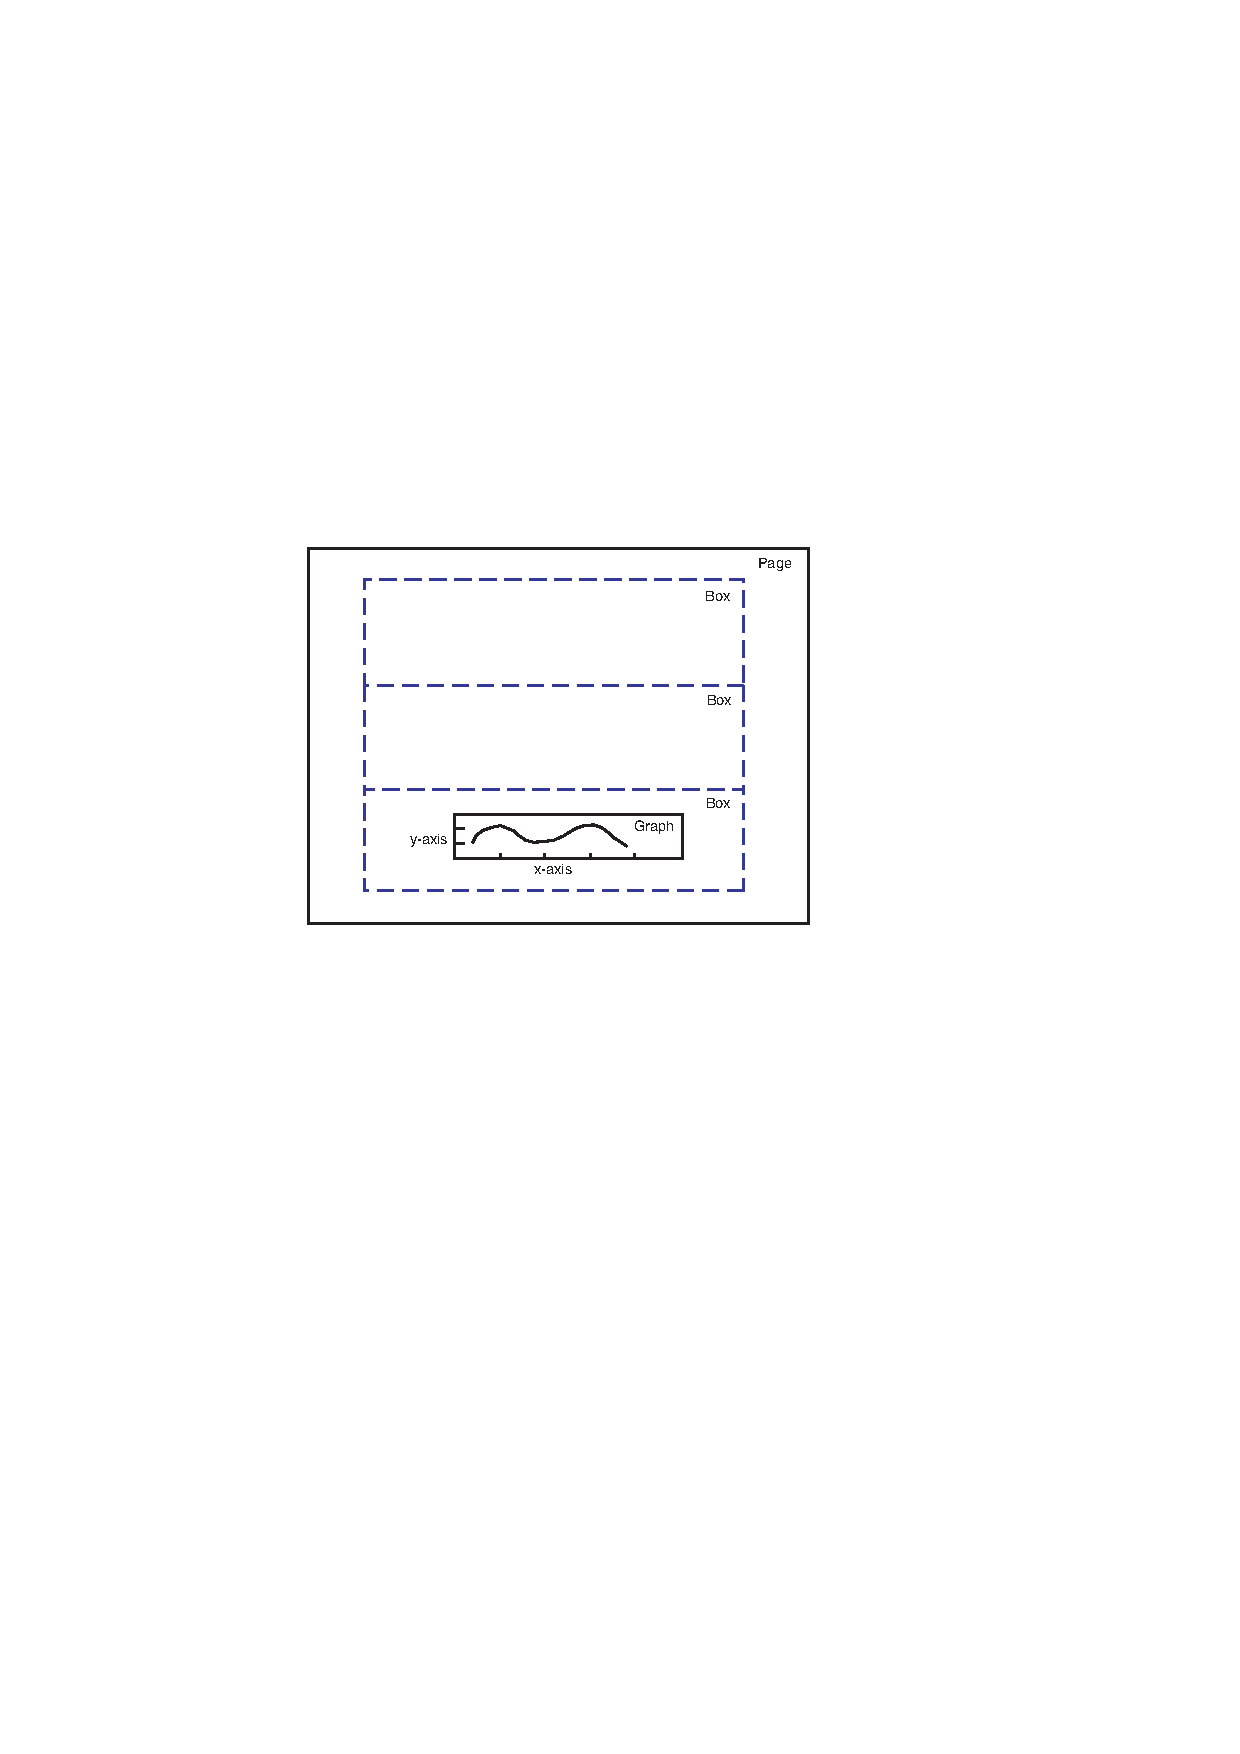
\includegraphics{plot_coords.psfig}
  \caption{A Graph within a Box within a Page.}
  \label{f:plot_coords}
\end{figure}

\quickplot uses the following concepts as shown in Figure~\ref{f:plot_coords}
\begin{example}
  PAGE  -- The entire drawing surface.
  BOX   -- The area of the page that a graph is placed into.
  GRAPH -- The actual plotting area within the bounds of the axes.
\end{example}
In case you need to refer to the PGPLOT routines the correspondence between this and PGPLOT is:
\begin{example}
  QUICK_PLOT    PGPLOT
  ----------    ------
  PAGE          VIEW SURFACE
  BOX           No corresponding entity.
  GRAPH         VIEWPORT and WINDOW
\end{example}
Essentially the VIEWPORT is the region outside of which lines and symbols
will be clipped (if clipping is turned on) and the WINDOW defines the
plot area. I'm not sure why PGPLOT makes a distinction but VIEWPORT and
WINDOW always are the same region.

\vn{qp_open_page} determines the size of the \vn{page} if it is settable (like for
X--windows). The page is divided up into a grid of boxes. For example, 
in Figure~\ref{f:plot_coords}, the grid is 1 box wide by 3 boxes tall. The border
between the grid of boxes and the edges of the page are set by \vn{qp_set_page_border}.
The box that the graph falls into is set by \vn{qp_set_box}. The default is to
have no margins with 1 box covering the entire page. The \vn{qp_set_margin} routine
sets the distance between the box edges and the axes.


%----------------------------------------------------------------------------
\section{Length and Position Units}
\label{s:plot_units}
\index{Quick_Plot!position units}

Typically there is an optional \vn{units} argument for \quickplot routines that
have length and/or position arguments. For example, using \vn{getf} one can
see that the arguments for \vn{qp_draw_rectangle} are
\begin{example}
  Subroutine qp_draw_rectangle (x1, x2, y1, y2, units, color, width, style, clip)
\end{example}
The \vn{units} argument is a character string which is divided into three
parts. The syntax of the \vn{units} argument is
\begin{example}
  unit_type/ref_object/corner
\end{example}
The first part \vn{unit_type} gives the type of units
\begin{example}
  "%"       -- Percent.
  "DATA"    -- Data units. (Draw default)
  "MM"      -- millimeters.
  "INCH"    -- Inches. (Set default)
  "POINTS"  -- Printers points (72 points = 1 inch, 1pt is about 1pixel).
\end{example}
The second and third parts give the reference point for a position.
The second part specifies the reference object
\begin{example}
    "PAGE"  -- Relative to the page (Set default).
    "BOX"   -- Relative to the box.
    "GRAPH" -- Relative to the graph (Draw default).
\end{example}
The third part gives corner of the reference object that is the reference point
\begin{example}
    "LB"    -- Left Bottom (Set and Draw default).
    "LT"    -- Left Top.
    "RB"    -- Right Bottom.
    "RT"    -- Right Top.
\end{example}

Notes:
\begin{itemize}
 \item 
The \vn{DATA} unit type, by definition, always uses the lower left
corner of the \vn{GRAPH} as a reference point.
 \item 
For the \vn{%} \vn{unit_type} the \vn{/} between \vn{unit_type} 
and \vn{ref_object} can be omitted.
 \item 
If the \vn{corner} is specified then the \vn{ref_object} must appear also.
 \item 
Everything must be in upper case.
 \item 
For some routines (\vn{qp_set_margin}, etc.) only a relative distance
is needed. In this case the \vn{ref_object/corner} part, if present,
is ignored.
 \item 
The \vn{units} argument is typically an optional argument. If not
present the default units will be used. There are actually two
defaults: The draw default is used for drawing text, symbols, or whatever.
The set default is used for setting margins, and other lengths.
Initially the draw default is \vn{DATA/GRAPH/LB} and the set
default is \vn{INCH/PAGE/LB}. use \vn{qp_set_default} to change this.
\end{itemize}
Examples:
\begin{example}
  "DATA"          -- This is the draw default. 
  "DATA/GRAPH/LB" -- Same as above.
  "DATA/BOX/RT"   -- ILLEGAL: DATA must always go with GRAPH/LB.
  "%PAGE/LT"      -- Percentage of page so (0.0, 1.0) = RT of page.
  "%BOX"          -- Percentage of box so (1.0, 1.0) = RT of box.
  "INCH/PAGE"     -- Inches from LB of page.
\end{example}

%----------------------------------------------------------------------------
\section{Y2 and X2 axes}
\label{s:axes2}
\index{Quick_Plot!axes}

The top and right axes of a graph are known as \vn{X2} and \vn{Y2}
respectively as shown in Figure~\ref{f:plot_coords}. Normally the
\vn{X2} axis mirrors the \vn{X} axis and the \vn{Y2} axis mirrors the
\vn{Y} axis in that the tick marks and axis numbering for the \vn{X2}
and \vn{Y2} axes are the same as the \vn{X} and \vn{Y} axes
respectively. \vn{qp_set_axis} can be used to disable mirroring. For example:
\begin{example}
  call qp_set_axis ("Y2", mirror = .false.)  ! y2-axis now independent of y.
\end{example}
\vn{qp_set_axis} can also be used to set \vn{Y2} axis parameters (axis
minimum, maximum, etc.). 

Note that the default is for the \vn{X2} and \vn{Y2} axis numbering
not to be shown. To enable or disable axis numbering again use
\vn{qp_set_axis}. For example:
\begin{example}
  call qp_set_axis ("Y2", draw_numbers = .true.)  ! draw y2 axis numbers
\end{example}

%----------------------------------------------------------------------------
\section{Styles}
\label{s:styles}

Symbolic constants have been defined for \quickplot subroutine
arguments that are used to choose various styles. As an example of
this is in lines 44 and 45 of Figure~\ref{f:plot_example}. The
numbers in the following are the PGPLOT equivalents.

\index{Quick_Plot!line styles}
The \quickplot line styles are:
\begin{example}
    1 -- solid\$                  Solid
    2 -- dashed\$                 Dashed
    3 -- dash_dot\$               Dash--dot 
    4 -- dotted\$                 Dotted
    5 -- dash_dot3\$              Dash--dot--dot--dot        
\end{example}

\index{Quick_Plot!color styles}
The color styles in \quickplot are:
\begin{example}
    0 -- White\$   (actually the background color)
    1 -- Black\$   (actually the foreground color)
    2 -- Red\$
    3 -- Green\$
    4 -- Blue\$
    5 -- Cyan\$
    6 -- Magenta\$
    7 -- Yellow\$ 
    8 -- Orange\$
    9 -- Yellow_Green\$
   10 -- Light_Green\$
   11 -- Navy_Blue\$
   12 -- Purple\$
   13 -- Redish_Purple\$
   14 -- Dark_Grey\$
   15 -- Light_Grey\$
\end{example}

\index{Quick_Plot!fill styles}
The fill styles are:
\begin{example}
    1 -- solid_fill\$        
    2 -- no_fill\$           
    3 -- hatched\$           
    4 -- cross_hatched\$     
\end{example}

\index{Quick_Plot!symbol table}
\begin{table}
  \centering
  \includegraphics{plot_syms.psfig}
  \caption{Plotting Symbols at Height = 40.0}
  \label{t:plot_syms}
\end{table}

\index{Quick_Plot!symbol styles}
The symbol types are:
\begin{example}
    0 -- square\$
    1 -- dot\$
    2 -- plus\$
    3 -- times\$
    4 -- circle\$
    5 -- x_symbol\$
    7 -- triangle\$
    8 -- circle_plus\$
    9 -- circle_dot\$
   10 -- square_concave\$
   11 -- diamond\$
   12 -- star5\$
   13 -- triangle_filled\$
   14 -- red_cross\$
   15 -- star_of_david\$
   16 -- square_filled\$
   17 -- circle_filled\$
   18 -- star5_filled\$
\end{example}
Beside this list, PGPLOT maps other numbers onto symbol types. 
The PGPLOT list of symbols is:
\begin{example}
  -3 ... -31 - a regular polygon with abs(type) edges.
          -2 - Same as -1.
          -1 - Dot with diameter = current line width.
   0 ...  31 - Standard marker symbols.
  32 ... 127 - ASCII characters (in the current font).
                  E.G. to use letter F as a marker, set type = ICHAR("F"). 
       > 127 - A Hershey symbol number.
\end{example}
Table~\ref{t:plot_syms} shows some of the symbols and there associated 
numbers. Note: At constant height PGPLOT gives symbols of different size.
To partially overcome this, \quickplot scales some of the symbols to
give a more uniform appearence. Table~\ref{t:plot_syms} was generated
using a height of 40 via the call
\begin{example}
  call qp_draw_symbol (0.5_rp, 0.5_rp, "%BOX", k, height = 40.0_rp)
\end{example}

PGPLOT defines certain escape sequences that can be used in text strings
to draw greek letters, etc. These escape sequences are given in 
Table~\ref{t:pgplot_escape}.
\begin{table}[h]
\begin{tabular}{|l|l|} \hline
{\B}u       & Start a superscript, or end a subscript \\ \hline
{\B}d       & \parbox{4in}{Start a subscript, or end a superscript 
               (note that {\B}u and {\B}d must always be used in pairs)} \\ \hline
{\B}b       & \parbox{4in}{Backspace (i.e., do not advance text pointer  
               after plotting the previous character)} \\ \hline
{\B}fn      & Switch to Normal font (1)       \\ \hline
{\B}fr      & Switch to Roman font (2)        \\ \hline
{\B}fi      & Switch to Italic font (3)       \\ \hline
{\B}fs      & Switch to Script font (4)       \\ \hline
{\B}{\B}    & Backslash character (\B)        \\ \hline
{\B}x       & Multiplication sign ($\times$)  \\ \hline
{\B}.       & Centered dot ($\cdot$)          \\ \hline
{\B}A       & Angstrom symbol (\AA)         \\ \hline
{\B}gx      & Greek letter corresponding to roman letter x \\ \hline
{\B}mn {\B}mnn & Graph marker number $n$ or $nn$ (1-31) \\ \hline
{\B}(nnnn)  & 
\parbox{4in}{Character number nnnn (1 to 4 decimal digits) from the
Hershey character set; the closing parenthesis may be omitted if the
next character is neither a digit nor ``)''. This makes a number of
special characters (e.g., mathematical, musical, astronomical, and
cartographical symbols) available.} \\ \hline
\end{tabular}
\caption{PGPLOT Escape Sequences.}
\label{t:pgplot_escape}
\end{table}

PGPLOT defines a text background index:
\begin{example}
         -1 - Transparent background.
          0 - Erase underlying graphics before drawing text.
   1 to 255 - Opaque with the number specifying the color index.
\end{example}

%----------------------------------------------------------------------------
\section{Structures}
\label{s:qp_structs}
\index{Quick_Plot!structures}

\quickplot uses several structures to hold data. The structure that
defines a line is called a \vn{qp_line_struct} and is shown in
Figure~\ref{f:qp_line_struct}. 
\begin{figure}[htb]
\centering
\begin{verbatim}
  type qp_line_struct
    integer width   ! Line width. Default = 1
    integer color   ! Line color. Default = black\$
    integer style   ! Line style. Default = solid\$
  end type
\end{verbatim}
\caption{Definition of the \vn{qp\_line\_struct}.}
\label{f:qp_line_struct}
\end{figure}

The \vn{qp_symbol_struct} defines how symbols are drawn and is shown
in Figure~\ref{f:qp_sym_struct}.
\begin{figure}[htb]
\centering
\begin{verbatim}
  type qp_symbol_struct
    integer  type        ! Default = circle_dot\$
    real(rp) height      ! Default = 6.0 (points)
    integer  color       ! Default = black\$
    integer  fill        ! Default = solid_fill\$
    integer  line_width  ! Default = 1
  end type
\end{verbatim}
\caption{Definition of the \vn{qp\_sym\_struct}.}
\label{f:qp_sym_struct}
\end{figure}

The \vn{qp_axis_struct} defines how axes are drawn and is shown
in Figure~\ref{f:qp_axis_struct}.
\begin{figure}[htb]
\centering
\begin{verbatim}
  type qp_axis_struct
    character(80) label       ! Axis label.
    real(rp) min              ! Axis minimum number.
    real(rp) max              ! Axis maximum number.
    real(rp) number_offset    ! Offset of numbering from the axis line.
    real(rp) label_offset     ! Offset of the label from the numbering.
    real(rp) major_tick_len   ! Length of the major ticks in inches.
    real(rp) minor_tick_len   ! Length of the minor ticks in inches.
    integer major_div         ! Number of major divisions.
    integer minor_div         ! Number of minor divisions.
    integer minor_div_max     ! Maximum number for auto choose.
    integer places            ! Places after the decimal point.
    character(16) type        ! For log scales. Not yet implemented.
    integer tick_side         ! +1 = draw to the inside, 0 = both, -1 = outside.
    integer number_side       ! +1 = draw to the inside, -1 = outside.
    logical draw_label        ! Draw the label?
    logical draw_numbers      ! Draw the numbering?
  end type
\end{verbatim}
\caption{Definition of the \vn{qp\_axis\_struct}.}
\label{f:qp_axis_struct}
\end{figure}



\chapter{Bmad Library Subroutine List}

Below are a list of \bmad\ and dcslib routines sorted by their
functionality.  Use the \vn{getf} and \vn{listf} (See section
\ref{s:getf}) scripts for more information on individual routines.
This list includes low level routines that are not generally used in
writing code for a program but may be useful in certain unique
situations.  Excluded from the list are low level routines that are
solely meant for \bmad\ internal use and specialized routines not of
general interest.


\toffset
\begin{center}
\begin{tabular}{|l|l|} \hline
{\em Routine Type} & {\em Section} \\ \hline
 	Reading/Writing Lattice Files           & \ref{r:read}       \\ \hline
 	Choosing a Lattice                      & \ref{r:lat}        \\ \hline
 	Twiss etc.                              & \ref{r:twiss}      \\ \hline
 	Matrices                                & \ref{r:mat}        \\ \hline
 	Routines called by \vn{make_mat6}       & \ref{r:mat6}       \\ \hline
 	Low level matrix routines               & \ref{r:low_mat}    \\ \hline
 	Tracking, Closed Orbit                  & \ref{r:track}      \\ \hline
 	Tracking Routines called by \vn{track1} & \ref{r:track1}     \\ \hline
 	Low Level Tracking Routines             & \ref{r:low_track}  \\ \hline
 	Particle Coordinate Stuff               & \ref{r:coord}      \\ \hline
 	Ring Geometry                           & \ref{r:geom}       \\ \hline
 	Interface to PTC                        & \ref{r:ptc}        \\ \hline
  \cpp interface                          & \ref{r:cpp}        \\ \hline
  Mad Tracking Routines                   & \ref{r:mad}        \\ \hline
 	Taylor Maps                             & \ref{r:taylor}     \\ \hline
  Macroparticle                           & \ref{r:macro}      \\ \hline
 	Long Range Beam--Beam Interaction       & \ref{r:lrbbi}      \\ \hline
 	Helper Routines: Informational          & \ref{r:info}       \\ \hline
 	Helper Routines: Elemental              & \ref{r:elem}       \\ \hline
 	Helper Routines: Transformational       & \ref{r:trans}      \\ \hline
 	Helper Routines: Multipoles             & \ref{r:multi}      \\ \hline
 	Helper Routines: Miscellaneous          & \ref{r:misc_help}  \\ \hline
 	Helper Routines: Low Level Stuff        & \ref{r:low_help}   \\ \hline
 	Overload Equal Sign Routines.           & \ref{r:equal}      \\ \hline
 	Linac Stuff (out of date)               & \ref{r:linac}      \\ \hline
 	CESR Specific                           & \ref{r:cesr}       \\ \hline
  Quick Plot                              & \ref{r:qp}         \\ \hline
  Nonlinear Optimizers                    & \ref{r:opti}       \\ \hline
  Miscellaneous DCSLIB Routines           & \ref{r:dcs_misc}   \\ \hline
 	Obsolete                                & \ref{r:obs}        \\ \hline
 	\end{tabular}
\end{center}
\toffset

%------------------------------------------------------------------------
\section{Reading/Writing Lattice Files} 
\label{r:read}

\begin{description}

\item[bmad\_parser (in\_file, ring)] \Newline
Subroutine to parse (read in) a Bmad input file. 

\item[bmad\_parser2 (in\_file, ring)] \Newline
Subroutine to parse (read in) a Bmad input file to modify an existing lattice. 

\item[bmad\_to\_mad (mad\_file, ring, ix\_start, ix\_end)] \Newline 
Subroutine to write a mad lattice file using the information in
a ring\_struct. 

\item[read\_digested\_bmad\_file (in\_file\_name, ring, version)] \Newline
Subroutine to read in a digested file. 

\item[write\_bmad\_lattice\_file (lattice\_name, ring)] \Newline 
Subroutine to write a Bmad lattice file using the information in
a ring\_struct.

\item[write\_digested\_bmad\_file (digested\_name, ring, n\_files, file\_names)] \Newline
Subroutine to write a digested file. 

\item[xsif\_parser (xsif\_file, ring, make\_mats6)] \Newline 
     Subroutine to parse an XSIF (extended standard input format) lattice file.

\end{description}

%------------------------------------------------------------------------
\section{Choosing a Lattice}
\label{r:lat}

\begin{description}

\item[choose\_cesr\_lattice (lattice, lat\_file, current\_lat, ring)] \Newline
Subroutine to let the user choose a lattice. The subroutine will present a list to choose from. 

\item[get\_lattice\_list (lat\_list, num\_lats, directory)] \Newline
Subroutine to get the names of the lattices of the form: directory/bmad\_*.lat 

\end{description}

%------------------------------------------------------------------------
\section{Twiss etc}
\label{r:twiss}

\begin{description}

\item[calc\_z\_tune (ring)] \Newline
Subroutine to calculate the synchrotron tune from the full 6X6 1 turn matrix. 

\item[chrom\_calc (ring, delta\_e, chrom\_x, chrom\_y)] \Newline
Subroutine to calculate the chromaticities by computing the tune 
change when then energy is changed. 

\item[chrom\_tune (ring, delta\_e, target\_x, target\_y, err\_flag)] \Newline
Subroutine to set the sextupole strengths so that the ring 
has the desired chromaticities. 

\item[emitt\_calc (ring, what, mode)] \Newline
Subroutine to calculate the emittance, energy spread, and synchrotron integrals. 

\item[quad\_beta\_ave (ring, ix\_ele, beta\_x\_ave, beta\_y\_ave)] \Newline
Subroutine to compute the average betas in a quad.

\item[radiation\_integrals (ring, orb\_, mode)] \Newline
Subroutine to calculate the synchrotron radiation integrals, the emittance, and energy spread. 

\item[relative\_mode\_flip (ele1, ele2)] \Newline
Function to see if the modes of ELE1 are flipped relative to ELE2. 

\item[set\_tune (phi\_x\_set, phi\_y\_set, dk1, ring, orb\_, ok)] \Newline
Subroutine to Q\_tune a ring. This routine will set the tunes to within 0.001 radian (0.06 deg). 

\item[set\_z\_tune (ring)] \Newline
Subroutine to set the longitudinal tune by setting the RF voltages in the RF cavities. 

\item[twiss\_and\_track (ring, orb)] \Newline
Subroutine to calculate the Twiss and orbit parameters. 
This is not necessarily the fastest routine. 

\item[twiss\_and\_track\_partial (ele1, ele2, param, del\_s, ele3, start, end)] \Newline
Subroutine to propagate partially through ELE2 the Twiss parameters and the orbit. 

\item[twiss\_at\_element (ring, ix\_ele, start, end, average)] \Newline
Subroutine to return the Twiss parameters at the beginning, end, or the average of an element. 

\item[twiss\_propagate\_many (ring, ix\_start, ix\_end, direction)] \Newline
Subroutine to propagate the Twiss parameters from one element in the ring to another. 

\item[twiss\_and\_track\_at\_s (ring, s, ele, orb\_, here)] \Newline
Subroutine to calculate the Twiss parameters and orbit at a particular longitudinal position. 

\item[twiss\_at\_start (ring)] \Newline
Subroutine to calculate the Twiss parameters at the start of the ring. 

\item[twiss\_from\_tracking (ring, closed\_orb\_, d\_orb, error)] \Newline
Subroutine to compute from tracking, for every element in the ring, 
the Twiss parameters and the transfer matrices. 

\item[twiss\_propagate1 (ele1, ele2)] \Newline
Subroutine to propagate the Twiss parameters from the end of ELE1 to the end of ELE2. 

\item[twiss\_propagate\_all (ring)] \Newline
Subroutine to propagate the Twiss parameters from the start to the end. 

\item[twiss\_to\_1\_turn\_mat (twiss, phi, mat2)] \Newline
Subroutine to form the 2x2 1-turn transfer matrix from the Twiss parameters. 

\end{description}

%------------------------------------------------------------------------
\section{Matrices}
\label{r:mat}

\begin{description}

\item[c\_to\_cbar (ele, cbar\_mat)] \Newline
Subroutine to compute Cbar from the C matrix and the Twiss parameters. 

\item[cbar\_to\_c (cbar\_mat, ele)] \Newline
Subroutine to compute C coupling matrix from the Cbar matrix and the Twiss parameters. 

\item[clear\_ring\_1turn\_mats (ring)] \Newline
Clear the 1-turn matrices in the ring structure. 

\item[do\_mode\_flip (ele, ele\_flip)] \Newline
Subroutine to mode flip the Twiss parameters of an element 

\item[make\_g2\_mats (twiss, g\_mat, g\_inv\_mat)] \Newline
Subroutine to make the matrices needed to go from normal mode coords to 
coordinates with the beta function removed. 

\item[make\_g\_mats (ele, g\_mat, g\_inv\_mat)] \Newline
Subroutine to make the matrices needed to go from normal mode coords to 
coordinates with the beta function removed. 

\item[make\_mat6 (ele, param, c0, c1)] \Newline
Subroutine to make the 6x6 transfer matrix for an element. 

\item[make\_v\_mats (ele, v\_mat, v\_inv\_mat)] \Newline
Subroutine to make the matrices needed to go from normal mode coords to X-Y 
coords and vice versa. 

\item[mat6\_to\_taylor (mat6, vec0, bmad\_taylor)] \Newline
Subroutine to form a first order Taylor map from the 6x6 transfer matrix 
and the 0th order transfer vector. 

\item[mat\_det (mat, det)] \Newline 
     Subroutine to take the determinant of a square matrix

\item[mat\_inverse (mat, mat\_inv)] \Newline
Suroutine to take the inverse of a square matrix. 

\item[mat\_make\_unit (mat)] \Newline 
     routine to create a unit matrix.

\item[mat\_rotation (mat, angle, bet\_1, bet\_2, alph\_1, alph\_2)] \Newline 
     Subroutine to construct a 2x2 rotation matrix for translation from
     point 1 to point 2.

\item[mat\_symplectify (mat\_in, mat\_symp)] \Newline
Subroutine to form a symplectic matrix that is approimately equal to the input matrix. 

\item[mat\_symp\_check (mat, error)] \Newline
Subroutine to check the symplecticity of a square matrix 

\item[mat\_symp\_decouple (t0, tol, stat, u, v, ubar, vbar, g, twiss1, twiss2, type\_out)] \Newline
Subroutine to find the symplectic eigen--modes of the one turn 4x4 coupled 
transfer matrix T0. 

\item[mat\_type (mat, nunit, header)] \Newline 
     Subroutine to output matrices to the terminal or to a file

\item[match\_ele\_to\_mat6 (ele, mat6, vec0)] \Newline 
Subroutine to make the 6 x 6 transfer matrix from the twiss parameters.

\item[multi\_turn\_tracking\_to\_mat (track, i\_dim, mat1, track0, chi)] \Newline
Subroutine to analyze 1-turn tracking data to find the 1-turn transfer matrix 
and the closed orbit offset.

\item[transfer\_matrix\_calc (ring, rf\_on, mat6, ix1, ix2)] \Newline
Subroutine to calculate the transfer matrix between two elements. If
ix1 and ix2 are not present the full 1--turn matrix is calculated.

\item[one\_turn\_mat\_at\_ele (ele, phi\_a, phi\_b, mat4)] \Newline
Subroutine to form the 4x4 1-turn coupled matrix with the reference point 
at the end of an element. 

\item[ring\_make\_mat6 (ring, ix\_ele, coord\_)] \Newline
Subroutine to make the 6x6 linear transfer matrix for an element 

\item[taylor\_to\_mat6 (a\_taylor, c0, mat6, c1)] \Newline
Subroutine to calculate the linear (Jacobian) matrix about some trajectory from a Taylor map. 

\item[transfer\_mat2\_from\_twiss (twiss1, twiss2, mat)] \Newline
Subroutine to make a 2 x 2 transfer matrix from the Twiss parameters at the end points. 

\item[transfer\_mat\_from\_twiss (ele1, ele2, m)] \Newline 
Subroutine to make a 6 x 6 transfer matrix from the twiss parameters
at the beginning and end of the element.

\item[twiss\_from\_mat2 (mat, det, twiss, stat, tol, type\_out)] \Newline
Subroutine to extract the Twiss parameters from the one-turn 2x2 matrix 

\item[twiss\_from\_mat6 (mat6, ele, stable, growth\_rate)] \Newline
Subroutine to extract the Twiss parameters from the one-turn 6x6 matrix 

\item[twiss\_to\_1\_turn\_mat (twiss, phi, mat2)] \Newline
Subroutine to form the 2x2 1-turn transfer matrix from the Twiss parameters. 

\end{description}

%------------------------------------------------------------------------
\section{Routines called by make\_mat6}
\label{r:mat6}

\begin{description}

\item[make\_mat6\_bmad (ele, param, c0, c1)] \Newline
Subroutine to make the 6x6 transfer matrix for an element
using closed formulas.

\item[make\_mat6\_custom (ele, param, c0, c1)] \Newline
Dummy routine for making the 6x6 transfer matrices.

\item[make\_mat6\_symp\_lie\_ptc (ele, param, c0, c1)] \Newline
Subroutine to make the 6x6 transfer matrix for an element using
the PTC symplectic integrator.

\item[make\_mat6\_taylor (ele, param, c0, c1)] \Newline
Subroutine to make the 6x6 transfer matrix for an element
from a Taylor map.

\item[make\_mat6\_tracking (ele, param, c0, c1)] \Newline
Subroutine to make the 6x6 transfer matrix for an element by 
tracking 7 particle with different starting conditions.

\end{description}

%------------------------------------------------------------------------
\section{Low Level Matrix Routines}
\label{r:low_mat}  

\begin{description}

\item[drift\_mat6\_calc (mat6, length, start, end)] \Newline
Subroutine to calculate a drift transfer matrix with a possible kick. 

\item[init\_lr\_wake (lr\_wake, n\_term)] \Newline 
Subroutine to initialize a lr\_wake array.

\item[init\_sr\_wake (sr\_wake, n\_term)] \Newline 
Subroutine to initialize a sr\_wake array.

\item[init\_wake (wake, n\_sr, n\_lr)] \Newline 
Subroutine to initialize a wake struct.

\item[lr\_wake\_array\_size (ele) result (array\_size)] \Newline 
Function to return the size of ele%wake%lr.

\item[mat6\_dispersion (mat6, e\_vec)] \Newline
Subroutine to put the dispersion into ELE%MAT6 given the dispersionvector E\_VEC 

\item[sol\_quad\_mat6\_calc (ks, k1, length, mat6, orb)] \Newline
Subroutine to calculate the transfer matrix for a combination solenoid/quadrupole element. 

\item[sr\_wake\_array\_size (ele) result (array\_size)] \Newline 
Function to return the size of ele%wake%sr.

\item[tilt\_mat6 (mat6, tilt)] \Newline
Subroutine to transform a 6x6 transfer matrix to a new reference frame that is 
tilted in (x, Px, y, Py) with respect to the old reference frame. 

\end{description}

%------------------------------------------------------------------------
\section{Tracking, Closed Orbit}
\label{r:track}    

\begin{description}

\item[check\_aperture\_limit (orb, ele, param)] \Newline
Subroutine to check if an orbit is outside the aperture. 

\item[closed\_orbit\_calc (ring, closed\_orb, i\_dim, direction)] \Newline 
Subroutine to calculate the closed orbit at the beginning of the ring.

\item[closed\_orbit\_from\_tracking (ring, closed\_orb\_, i\_dim, 
eps\_rel, eps\_abs, init\_guess)] \Newline
Subroutine to find the closed orbit via tracking. 

\item[dynamic\_aperture (ring, track\_input, aperture)] \Newline
Subroutine to determine the dynamic aperture of a lattice via tracking. 

\item[lost\_particle\_info (lattice, orbit, ix\_lost, plane\_lost)] \Newline 
Subroutine to show where in an orbit a particle hit an aperture and was lost.

\item[multi\_turn\_tracking\_analysis (track, i\_dim, track0, ele, 
stable, growth\_rate, chi)] \Newline
Subroutine to analyze multi-turn tracking data to get the Twiss
parameters etc.

\item[multi\_turn\_tracking\_to\_mat (track, i\_dim, 
mat1, track0, chi)] \Newline
Subroutine to analyze 1-turn tracking data to find the 1-turn transfer
matrix and the closed orbit offset.

\item[\protect\parbox{6in}{offset\_particle (ele, param, coord, set, 
set\_canonical, \\
\hspace*{2in} set\_tilt, set\_multipoles, set\_hvkicks, s\_pos)}] \Newline
Subroutine to effectively offset an element by instead offsetting 
the particle position to correspond to the local element coordinates. 

\item[orbit\_amplitude\_calc (ele, orb, amp\_a, amp\_b, amp\_na, amp\_nb, particle)] \Newline
Routine to calculate the "invariant" amplitude of a particle at a 
particular point in its orbit. 

\item[setup\_radiation\_tracking (ring, closed\_orb, fluctuations\_on, damping\_on)] \Newline
Subroutine to compute synchrotron radiation parameters prior to tracking. 

\item[tilt\_coords (tilt\_val coord, set)] \Newline
Subroutine to effectively tilt (rotate in the x-y plane) an element by 
instead rotating the particle position with negative the angle. 

\item[track1 (start, ele, param, end)] \Newline
Subroutine to track through a single element. 

\item[track\_all (ring, orbit\_)] \Newline
Subroutine to track through the ring. 

\item[track\_beam (ring, beam, ix1, ix2)] \Newline 
     Subroutine to track a beam of macroparticles from the end of
     ring%ele\_(ix1) Through to the end of ring%ele\_(ix2).

\item[track\_many (ring, orbit\_, ix\_start, ix\_end, direction)] \Newline
Subroutine to track from one element in the ring to another. 

\item[twiss\_and\_track (ring, orb)] \Newline
See the Twiss section for more details. 

\item[twiss\_and\_track\_at\_s (ring, s, ele, orb\_, here)] \Newline
Subroutine to calculate the Twiss parameters and orbit at a particular longitudinal position. 

\item[twiss\_and\_track\_partial (ele1, ele2, param, del\_s, ele3, start, end)] \Newline
Subroutine to calculate the Twiss parameters and orbit at a particular position inside an element. 

\item[twiss\_from\_tracking (ring, closed\_orb\_, d\_orb, error)] \Newline
Subroutine to compute from tracking the Twiss parameters and the transfer matrices 
for every element in the ring. 

\end{description}

%------------------------------------------------------------------------
\section{Tracking Routines called by TRACK1}
\label{r:track1}   

Note: Generally you don't call these routines directly.

\begin{description}

\item[symp\_lie\_bmad (ele, param, start, end, calc\_mat6)] \Newline
Symplectic integration through an element to 0th or 1st order.

\item[track1\_adaptive\_boris (start, ele, param, end, s\_start, s\_end)] \Newline
Subroutine to do Boris tracking with adaptive step size control. 

\item[track1\_boris (start, ele, param, end, s\_start, s\_end)] \Newline
Subroutine to do Boris tracking.  

\item[track1\_bmad (start, ele, param, end)] \Newline
Particle tracking through a single element BMAD\_standard style. 

\item[track1\_custom (start, ele, param, end)] \Newline
Dummy routine for custom\_tracking.

\item[track1\_linear (start, ele, param, end)] \Newline
Particle tracking through a single element using the tranfer matrix.. 

\item[track1\_radiation (start, ele, param, end, edge)] \Newline
Subroutine to put in radiation damping and/or fluctuations. 

\item[track1\_runge\_kutta (start, ele, param, end)] \Newline
Subroutine to do tracking using Runge-Kutta integration. 

\item[track1\_symp\_lie\_ptc (start, ele, param, end)] \Newline
Particle tracking through a single element using a Hamiltonian and a 
symplectic integrator. 

\item[track1\_symp\_map (start, ele, param, end)] \Newline
Particle tracking through a single element using a partially inverted 
taylor map (In PTC/FPP this is called a genfield). 

\item[track1\_taylor (start, ele, param, end)] \Newline
Subroutine to track through an element using the elements taylor series. 

\item[track1\_wiedemann\_wiggler (start, ele, param, end)] \Newline
Subroutine to track through the body of a wiggler. 

\end{description}

%------------------------------------------------------------------------
\section{Low Level Tracking Routines}
\label{r:low_track}

\begin{description}

\item[odeint\_bmad (start, ele, param, end, s1, s2, rel\_tol, abs\_tol, h1, hmin)] \Newline
Subroutine to do Runge Kutta tracking. 

\item[track\_a\_accel\_sol (start, ele, param, end)] \Newline
Subroutine to track through an accel\_sol element.

\item[track1\_boris\_partial (start, ele, param, s, ds, end)] \Newline
Subroutine to track 1 step using boris tracking. 
This subroutine is used by track1\_boris and track1\_adaptive\_boris. 

\item[track\_a\_drift (orb, length)] \Newline
Subroutine to track through a drift. 

\item[track\_a\_bend (start, ele, param, end)] \Newline
Particle tracking through a bend element. 

\end{description}

%------------------------------------------------------------------------
\section{Particle Coordinate Stuff}
\label{r:coord}    

\begin{description}

\item[convert\_coords (in\_type\_str, coord\_in, ele, out\_type\_str, coord\_out)] \Newline
Subroutine to convert between lab frame, normal mode, normalized normal mode, 
and action-angle coordinates. 

\item[type\_coord (coord)] \Newline
Subroutine to type out a coordinate. 

\end{description}

%------------------------------------------------------------------------
\section{Ring Geometry}
\label{r:geom}     

\begin{description}

\item[ring\_geometry (ring)] \Newline
Subroutine to calculate the physical placement of all the elements in a ring. 
That is, the layout on the floor. 

\item[s\_calc (ring)] \Newline
Subroutine to calculate the longitudinal distance S for the elements in a ring. 

\end{description}

%------------------------------------------------------------------------
\section{Interface to PTC}
\label{r:ptc}      

\begin{description}

\item[concat\_real\_8 (y1, y2, y3)] \Newline
Subroutine to concatenate two real\_8 taylor series. 

\item[ele\_to\_fibre (ele, fiber, param, integ\_order, steps)] \Newline
Subroutine to convert a Bmad element to a PTC fibre element. 

\item[map\_coef(y, i, j, k, l, style)] \Newline
Function to return the coefficient of the map y(:) up to 3rd order. 

\item[kill\_gen\_field (gen\_field)] \Newline
Subroutine to kill a gen\_field. 

\item[kind\_name (this\_kind)] \Newline
Function to return the name of a PTC kind. 

\item[real\_8\_equal\_taylor (y8, bmad\_taylor)] \Newline
Subroutine to overload "=" in expressions real\_8 = bmad\_taylor 

\item[real\_8\_to\_taylor (y8, bmad\_taylor, switch\_z)] \Newline
Subroutine to convert from a real\_8 taylor map in Etienne's PTC to a taylor map in Bmad. 

\item[real\_8\_init (y, set\_taylor)] \Newline
Subroutine to allocate a PTC real\_8 variable. 

\item[remove\_constant\_taylor (taylor\_in, taylor\_out, c0, remove\_higher\_order\_terms)] \Newline
Subroutine to remove the constant part of a taylor series. 

\item[ring\_to\_layout (ring, ptc\_layout)] \Newline
Subroutine to create a PTC layout from a Bmad ring. 

\item[set\_ptc (param, taylor\_order, integ\_order, num\_steps, no\_cavity, exact\_calc)] \Newline
Subroutine to initialize PTC. 

\item[set\_taylor\_order (order, override\_flag)] \Newline
Subroutine to set the taylor order. 

\item[sort\_universal\_terms (ut\_in, ut\_sorted)] \Newline
Subroutine to sort the taylor terms from "lowest" to "highest". 

\item[taylor\_equal\_real\_8 (bmad\_taylor, y8)] \Newline
Subroutine to overload "=" in expressions bmad\_taylor = y8 

\item[taylor\_to\_real\_8 (bmad\_taylor, y8, switch\_z)] \Newline
Subroutine to convert from a taylor map in Bmad to a real\_8 taylor map in Etienne's PTC. 

\item[type\_layout (lay)] \Newline
Subroutine to print the global information in a PTC layout.

\item[type\_map1 (y, type0, n\_dim, style)] \Newline
Subroutine to type the transfer map up to first order. 

\item[type\_fibre (fib)] \Newline
Subroutine to print the global information in a fibre.

\item[type\_map (y)] \Newline
Subroutine to type the transfer maps of a real\_8 array. 

\item[type\_real\_8\_taylors (y, switch\_z)] \Newline
Subroutine to type out the taylor series from a real\_8 array. 

\item[taylor\_to\_genfield (bmad\_taylor, gen\_field, c0)] \Newline
Subroutine to construct a genfield (partially inverted map) from a taylor map. 

\item[universal\_to\_bmad\_taylor (u\_taylor, bmad\_taylor, switch\_z)] \Newline
Subroutine to convert from a universal\_taylor map in Etienne's PTC to a taylor map in Bmad. 

\item[vec\_bmad\_to\_ptc (vec\_bmad, vec\_ptc)] \Newline
Subroutine to convert from Bmad to PTC coordinates. 

\item[vec\_ptc\_to\_bmad (vec\_ptc, vec\_bmad)] \Newline
Subroutine to convert from PTC to Bmad coordinates. 

\end{description}

%------------------------------------------------------------------------
\section{C++ Interface}
\label{r:cpp}      
\index{C++ interface!routines}

\begin{description}

\item[amode\_to\_c (f\_amode, c\_amode)] \Newline 
Subroutine to convert a Bmad amode\_struct to a C++ C\_amode.

\item[arr2mat (arr, n1, n2) result (mat)] \Newline 
Function to take a an array and turn it into a matrix.

\item[bmad\_com\_to\_c (c\_bmad\_com)] \Newline 
Subroutine to convert the Bmad bmad\_com\_struct common block to 
a C++ C\_bmad\_com.

\item[c\_logic (logic) result (c\_log)] \Newline 
Function to convert from a fortran logical to a C logical.

\item[c\_str (str) result (c\_string)] \Newline 
Function to append a null (0) character at the end of a string (trimmed
of trailing blanks) so it will look like a C character array. 

\item[control\_to\_c (f\_control, c\_control)] \Newline 
Subroutine to convert a Bmad control\_struct to a C++ C\_control.

\item[coord\_to\_c (f\_coord, c\_coord)] \Newline 
Subroutine to convert a Bmad coord\_struct to a C++ C\_coord.

\item[ele\_to\_c (f\_ele, c\_ele)] \Newline 
Subroutine to convert a Bmad ele\_struct to a C++ C\_ele.

\item[em\_field\_to\_c (f\_em\_field, c\_em\_field)] \Newline 
Subroutine to convert a Bmad em\_field\_struct to a C++ C\_em\_field.

\item[f\_logic (logic) result (f\_log)] \Newline 
Function to convert from a fortran logical to a C logical.

\item[floor\_position\_to\_c (f\_floor\_position, c\_floor\_position)] \Newline 
Subroutine to convert a Bmad floor\_position\_struct to a C++ C\_floor\_position.

\item[linac\_mode\_to\_c (f\_linac\_mode, c\_linac\_mode)] \Newline 
Subroutine to convert a Bmad linac\_mode\_struct to a C++ C\_linac\_mode.

\item[lr\_wake\_to\_c (f\_lr\_wake, c\_lr\_wake)] \Newline 
Subroutine to convert a Bmad lr\_wake\_struct to a C++ C\_lr\_wake.

\item[mat2arr (mat) result (arr)] \Newline 
Function to take a matrix and turn it into an array.

\item[modes\_to\_c (f\_modes, c\_modes)] \Newline 
Subroutine to convert a Bmad modes\_struct to a C++ C\_modes.

\item[mode\_info\_to\_c (f\_mode\_info, c\_mode\_info)] \Newline 
Subroutine to convert a Bmad mode\_info\_struct to a C++ C\_mode\_info.

\item[orbit\_to\_c (f\_orbit, c\_orbit)] \Newline 
Subroutine to convert an a Bmad orbit\_struct to a C++ C\_orbit.

\item[param\_to\_c (f\_param, c\_param)] \Newline 
Subroutine to convert a Bmad param\_struct to a C++ C\_param.

\item[ring\_to\_c (f\_ring, c\_ring)] \Newline 
Subroutine to convert a Bmad ring\_struct to a C++ C\_ring.

\item[sr\_wake\_to\_c (f\_sr\_wake, c\_sr\_wake)] \Newline 
Subroutine to convert a Bmad sr\_wake\_struct to a C++ C\_sr\_wake.

\item[twiss\_to\_c (f\_twiss, c\_twiss)] \Newline 
Subroutine to convert a Bmad twiss\_struct to a C++ C\_twiss.

\item[taylor\_term\_to\_c (f\_taylor\_term, c\_taylor\_term)] \Newline 
Subroutine to convert a Bmad taylor\_term\_struct to a C++ C\_taylor\_term.

\item[taylor\_to\_c (f\_taylor, c\_taylor)] \Newline 
Subroutine to convert a Bmad taylor\_struct to a C++ C\_taylor.

\item[wake\_to\_c (f\_wake, c\_wake)] \Newline 
Subroutine to convert a Bmad wake\_struct to a C++ C\_wake.

\item[wig\_term\_to\_c (f\_wig\_term, c\_wig\_term)] \Newline 
Subroutine to convert a Bmad wig\_term\_struct to a C++ C\_wig\_term.

\end{description}

%------------------------------------------------------------------------
\section{Mad Tracking Routines}
\label{r:mad}      

\begin{description}

\item[make\_mat6\_mad (ele, param, map, c0, c1)] \Newline 
     Subroutine to make the 6x6 transfer matrix for an element from the 
     2nd order MAD transport map. The map is stored in ele%taylor.

\item[make\_mad\_map (ele, particle, map)] \Newline 
     Subroutine to make a 2nd order transport map a la MAD.

\item[mad\_add\_offsets\_and\_multipoles (ele, energy, map)] \Newline 
     Subroutine to add in the effect of element offsets and/or multipoles
     on the 2nd order transport map for the element.

\item[mad\_drift (ele, energy, map)] \Newline 
     Subroutine to make a transport map for a drift space.
     The equivalent MAD-8 routine is: TMDRF

\item[mad\_elsep (ele, energy, map)] \Newline 
     Subroutine to make a transport map for an electric separator. 
     The equivalent MAD-8 routine is: TMSEP

\item[mad\_sextupole (ele, energy, map)] \Newline 
     Subroutine to make a transport map for an sextupole.
     The equivalent MAD-8 routine is: TMSEXT

\item[mad\_sbend (ele, energy, map)] \Newline 
     Subroutine to make a transport map for a sector bend element.
     The equivalent MAD-8 routine is: TMBEND

\item[mad\_sbend\_fringe (ele, energy, into, map)] \Newline 
     Subroutine to make a transport map for the fringe field of a dipole.
     The equivalent MAD-8 routine is: TMFRNG

\item[mad\_sbend\_body (ele, energy, map)] \Newline 
     Subroutine to make a transport map for the body of a sector dipole.
     The equivalent MAD-8 routine is: TMSECT

\item[mad\_tmfoc (el, sk1, c, s, d, f) ] \Newline 
     Subroutine to compute the linear focussing functions.  
     The equivalent MAD-8 routine is: TMFOC

\item[mad\_quadrupole (ele, energy, map)] \Newline 
     Subroutine to make a transport map for an quadrupole element.
     The equivalent MAD-8 routine is: TMSEXT

\item[mad\_rfcavity (ele, energy, map)] \Newline 
     Subroutine to make a transport map for an rfcavity element.
     The equivalent MAD-8 routine is: TMRF

\item[mad\_solenoid (ele, energy, map)] \Newline 
     Subroutine to make a transport map for an solenoid.
     The equivalent MAD-8 routine is: TMSEXT

\item[mad\_sol\_quad (ele, energy, map)] \Newline 
     Subroutine to make a transport map for a combination solenoid/quadrupole.
     Note: There is no equivalent MAD-8 routine.

\item[mad\_tmsymm (te)] \Newline 
     subroutine to symmertrize the 2nd order map t.
     The equivalent MAD-8 routine is: tmsymm

\item[mad\_tmtilt (map, tilt)] \Newline 
     Subroutine to apply a tilt to a transport map.
     The equivalent MAD-8 routine is: TMTILT

\item[mad\_concat\_map2 (map1, map2, map3)] \Newline 
     Subroutine to concatinate two 2nd order transport maps.
         map3 = map2(map1)

\item[mad\_track1 (c0, map, c1)] \Newline 
     Subroutine to track through a 2nd order transfer map.
     The equivalent MAD-8 routine is: TMTRAK

\item[track1\_mad (start, ele, param, end)] \Newline 
     Subroutine to track through an element using a 2nd order transfer map.
     Note: If map does not exist then one will be created. 

\item[mad\_map\_to\_taylor (map, taylor)] \Newline 
     Subroutine to convert a mad order 2 map to a taylor map.

\item[taylor\_to\_mad\_map (taylor, map)] \Newline 
     Subroutine to convert a Taylor map to a mad order 2 map.
     If any of the Taylor terms have order greater than 2 they are ignored.

\item[make\_unit\_mad\_map (map)] \Newline 
     Subroutine to initialize a 2nd order transport map to unity.


\end{description}

%------------------------------------------------------------------------
\section{Taylor Map Routines}
\label{r:taylor}   

\begin{description}

\item[concat\_taylor (taylor1, taylor2, taylor3)] \Newline
Subroutine to concatenate two taylor series: taylor3(x) = taylor1(taylor2(x)) 

\item[ele\_to\_taylor (ele, param, orb0)] \Newline
Subroutine to make a Taylor map for an element. The order of the map is set by set\_ptc.

\item[equivalent\_eles (ele1, ele2) result (equiv)] \Newline 
Subroutine to see if to elements are equivalent in terms of attributes so
that their Taylor Maps would be the same. 

\item[init\_taylor (bmad\_taylor)] \Newline
Subroutine to initialize (nullify) a Bmad Taylor map. 

\item[kill\_taylor (bmad\_taylor)] \Newline
Subroutine to deallocate a Bmad Taylor map. 

\item[mat6\_to\_taylor (mat6, vec0, bmad\_taylor)] \Newline
Subroutine to form a first order Taylor map from the 6x6 transfer matrix 
and the 0th order transfer vector. 

\item[set\_taylor\_order (order, override\_flag)] \Newline
Subroutine to set the taylor order. 

\item[sort\_taylor\_terms (taylor\_in, taylor\_sorted)] \Newline
Subroutine to sort the taylor terms from "lowest" to "highest" of a Taylor series. 

\item[taylor\_coef (bmad\_taylor, exp)] \Newline 
Function to return the coefficient for a particular taylor term from a Taylor Series.

\item[taylor\_equal\_taylor (taylor1, taylor2)] \Newline
Subroutine to transfer the values from one taylor map to another: Taylor1 $\le$ Taylor2 

\item[taylors\_equal\_taylors (taylor1, taylor2)] \Newline 
Subroutine to transfer the values from one taylor map to another.

\item[taylor\_to\_mat6 (a\_taylor, c0, mat6, c1)] \Newline
Subroutine to calculate the linear (Jacobian) matrix about some trajectory from a Taylor map. 

\item[taylor\_inverse (taylor\_in, taylor\_inv)] \Newline
Subroutine to invert a taylor map. 

\item[taylor\_propagate1 (tlr, ele, param)] \Newline
Subroutine to track a real\_8 taylor map through an element. 
The alternative routine, if ele has a taylor series, is concat\_taylor. 

\item[track\_taylor (start, bmad\_taylor, end)] \Newline
Subroutine to track using a Taylor map. 

\item[transfer\_ele\_taylor (ele\_in, ele\_out, taylor\_order)] \Newline 
Subroutine to transfer a Taylor map from one element to another.

\item[transfer\_ring\_taylors (ring\_in, ring\_out, 
                                             type\_out, transfered\_all) ] \Newline 
Subroutine to transfer the taylor maps from the elements of one ring to
the elements of another. 

\item[type\_taylors (bmad\_taylor)] \Newline
Subroutine to print in a nice format a Bmad taylor map at the terminal. 

\item[type2\_taylors (bmad\_taylor, lines, n\_lines)] \Newline
Subroutine to write a Bmad taylor map in a nice format to a character array. 

\end{description}

%------------------------------------------------------------------------
\section{Macroparticle Routines}
\label{r:macro}    

\begin{description}

\item[calc\_bunch\_centroid (bunch, params)] \Newline
Subroutine to calculate bunch centroid and total charge excluding lost
macroparticles.

\item[calc\_bunch\_dpz\_dz (bunch, params, calc\_centroid)] \Newline
Subroutine to calculate bunch energy-Z correlation.

\item[calc\_bunch\_params (bunch, ele, params)] \Newline
Subroutine to calculate various beam characteristics from a bunch.

\item[calc\_bunch\_sigma (bunch, params, calc\_centroid)] \Newline
Subrouine to calculate bunch sigmas.

\item[calc\_bunch\_twiss\_and\_emittance (bunch, ele, params, calc\_centroid)] \Newline 
Subroutine to calculate the beam twiss parameters and normalized emittances of a bunch.

\item[init\_macro\_distribution (beam, init, canonical\_out)] \Newline 
Subroutine to initialize a macroparticle distribution.
This routine uses the LIAR algorithm. See the Bmad manual for more details.

\item[mat\_to\_mp\_sigma (mat, sigma)] \Newline 
Subroutine to convert a sigma matrix. to a linear array of 
macroparticle sigmas.

\item[mp\_sigma\_to\_mat (sigma, mat)] \Newline 
Subroutine to convert a linear array of macroparticle sigmas to a 
sigma matrix. 

\item[mp\_to\_angle\_coords (mp, energy0)] \Newline 
Subroutine to convert macroparticle coords from 
(x, px, y, py, z, pz) to (x, x', y, y', z, E).

\item[mp\_to\_canonical\_coords (mp, energy0)] \Newline 
Subroutine to convert macroparticle coords from 
(x, x', y, y', z, E) to (x, px, y, py, z, pz).

\item[reallocate\_beam (beam, n\_bunch, n\_slice, n\_macro)] \Newline 
Subroutine to reallocate memory within a beam\_struct.

\item[track1\_beam (start, ele, param, end] \Newline
Subroutine to track a beam of macroparticles through an element.

\item[track\_beam (ring, beam, ix1, ix2)] \Newline 
Subroutine to track a beam of macroparticles from the end of
ring%ele\_(ix1) Through to the end of ring%ele\_(ix2).

\item[track1\_macroparticle (start, ele, param, end)] \Newline 
Subroutine to track a macroparticle through an element.


\end{description}

%------------------------------------------------------------------------
\section{Long Range Beam-Beam Interaction}
\label{r:lrbbi}    

\begin{description}

\item[init\_lrbbi(ring, oppos\_ring, lrbbi\_ele, ix\_lrbbi, ix\_oppos)] \Newline 
     Subroutine to calculate the basic parameters of a beambeam element. 
     Initializes the element and establishes the following values.

\item[insert\_lrbbi (ring, ring\_oppos, cross\_positions, ix\_lrbbi)] \Newline
Subroutine to create and insert beambeam elements at each parasitic crossing
point as specified form a list of crossing points.

\item[lrbbi\_crossings (n\_bucket, oppos\_buckets, cross\_positions)] \Newline
Subroutine to calculate the location of the parasitic crossings points 
given a bunch and an array of positions of the bunches it will cross. 

\item[make\_lrbbi(master\_ring, master\_ring\_oppos, ring, ix\_lrbbi, master\_ix\_lrbbi)] \Newline
Subroutine to turn elements marking parasitic crossings into beam-beam elements. 

\item[mark\_lrbbi(master\_ring, master\_ring\_oppos, ring, crossings)] \Newline
Subroutine to insert named markers into the ring structure at the positions of parasitic crossings. 

\end{description}

%------------------------------------------------------------------------
\section{Helper Routines: Informational}
\label{r:info}     

\begin{description}

\item[attribute\_index (key, name)] \Newline
Function to return the index of an attribute for a given element 
type and the name of the attribute 

\item[attribute\_name (key, index)] \Newline
Function to return the name of an attribute for a particular type of element. 

\item[check\_ring\_controls (ring, exit\_on\_error)] \Newline
Subroutine to check if the control links in a ring structure are valid. 

\item[check\_attrib\_free (ele, ix\_attrib, ring, err\_flag, err\_print\_flag)] \Newline
Subroutine to check if an attribute is free to vary.

\item[elements\_locator (key, ring, indx)] \Newline
Subroutine to locate all the elements of a certain kind in a ring. 

\item[element\_locator (ele\_name, ring, ix\_ele)] \Newline
Subroutine to locate an element in a ring. 

\item[equivalent\_eles (ele1, ele2) result (equiv)] \Newline 
Subroutine to see if twoo elements are equivalent in terms of their attributes so
that their Taylor Maps, if they existed, would be the same.

\item[find\_element\_ends (ring, ix\_ele, ix\_start, ix\_end)] \Newline
Subroutine to find the end points of an element. 

\item[type\_ele (ele, type\_zero\_attrib, type\_mat6, type\_twiss, 
type\_control)] \Newline
Subroutine to print the contents of an element at the terminal. 

\item[type2\_ele (ele, type\_zero\_attrib, type\_mat6, type\_twiss, 
type\_control, lines, n\_lines)] \Newline
Like \vn{type_ele} but the output is stored in a string array. 

\item[type\_twiss (ele, frequency\_units)] \Newline
Subroutine to type out the Twiss parameters from an element. 

\item[type2\_twiss (ele, frequency\_units, lines, n\_lines)] \Newline
Like \vn{type_twiss} but the output is stored in a string array. 

\end{description}

%------------------------------------------------------------------------
\section{Helper Routines: Elemental}
\label{r:elem}     

These routine are for adding elements, moving elements, etc.

\begin{description}

\item[add\_superimpose (ring, super\_ele, ix\_super)] \Newline
Subroutine to make a superimposed element. 

\item[attribute\_bookkeeper (ele, param)] \Newline
Subroutine to make sure the attributes of an element are self-consistent. 

\item[change\_basis (coord, ref\_energy, ref\_z, to\_cart, time\_disp)] \Newline
Subroutine to convert accelerator coordinates (x, x', y, y', z, z') to
Cartesian coordinates and time derivatives (x, x\_dot, y, y\_dot, z,
z\_dot) or vice-versa.

\item[create\_group (ring, ix\_ele, contrl)] \Newline
Subroutine to create a group control element. 

\item[create\_i\_beam (ring, ix\_i\_beam, ix\_slave\_)] \Newline 
     Subroutine to add the controller information to slave elements of
     an i\_beam\_lord.

\item[create\_overlay (ring, ix\_overlay, attrib\_name, , contl)] \Newline
Subroutine to add the controller information to slave elements of an 
overlay\_lord. 

\item[compress\_ring (ring, ok)] \Newline
Subroutine to compress the ele\_(*) and control\_(*) arrays to remove
elements no longer used.

\item[insert\_element (ring, insert\_ele, insert\_index)] \Newline
Subroutine to Insert a new element into the regular part of the ring structure. 

\item[make\_hybrid\_ring (ring\_in, use\_ele, remove\_markers, ring\_out, ix\_out)] \Newline
Subroutine to concatenate together elements to make a hybrid ring 

\item[new\_control (ring, ix\_ele)] \Newline
Subroutine to create a new control element. 

\item[\protect\parbox{6in}{pointer\_to\_attribute (ele, attrib\_name, do\_allocation, 
\\ \hspace*{2in} ptr\_attrib, ix\_attrib, err\_flag, err\_print\_flag)}] \Newline
Returns a pointer to an attribute of an element with name attrib\_name. 

\item[set\_ele\_attribute (ring, i\_ele, attrib\_name, attrib\_value, 
err\_flag, make\_mat6\_flag, orbit\_)] \Newline
Subroutine to set the attribute of an element and propagate the change to any slave elements. 

\item[split\_ring (ring, s\_split, ix\_split, split\_done)] \Newline
Subroutine to split a ring at a point.

\item[update\_hybrid\_list (ring, n\_in, use\_ele)] \Newline
Subroutine used to specify a list of element that should not be
hyberdized by \vn{make_hybrid_ring}.

\end{description}

%------------------------------------------------------------------------
\section{Helper Routines: Transformational}
\label{r:trans}    

\begin{description}

\item[adjust\_control\_struct (ring, ix\_ele)] \Newline
Subroutine to adjust the control structure of a ring so that 
extra control elements can be added. 

\item[allocate\_ring\_ele\_(ring, des\_size)] \Newline 
Subroutine to allocate or re-allocate the ring%ele\_(:) pointer in a ring.

\item[control\_bookkeeper (ring, ix\_ele)] \Newline
Subroutine to calculate the combined strength of the attributes for
controlled elements.

\item[deallocate\_ring\_pointers (ring)] \Newline 
Subroutine to deallocate the pointers in a ring.

\item[init\_ele (ele)] \Newline
Subroutine to initialize an element. 

\item[init\_ring (ring, n)] \Newline 
Subroutine to initialize a Bmad ring.

\item[lattice\_bookkeeper (ring)] \Newline 
Subroutine to do bookkeeping for the entire lattice.

\item[reallocate\_coord (coord\_, n\_coord)] \Newline 
Subroutine to reallocate an allocatable  coord\_struct array to at least:
coord\_(0:n\_coord).

\item[reverse\_ele (ele)] \Newline
Subroutine to "reverse" an element for backward tracking. 

\item[ring\_reverse (ring\_in, ring\_rev)] \Newline
Subroutine to construct a ring structure with the elements in reversed 
order. This may be used for backward tracking through the ring. 

\item[set\_design\_linear (ring)] \Newline
Subroutine to set only those elements on that constitute the "design" 
lattice. That is, only quadrupoles, bends and wigglers will be set on. 

\item[set\_on\_off (key, ring, switch, orb\_)] \Newline
Subroutine to turn on or off a set of elements (quadrupoles,
rfcavities, etc.) in a ring.

\item[transfer\_ele (ele1, ele2)] \Newline 
     Subroutine to set ele2 = ele1. 
     This is a plain transfer of information not using the overloaded equal.

\item[transfer\_eles (ele1, ele2)] \Newline 
     Subroutine to set ele2(:) = ele1(:). 
     This is a plain transfer of information not using the overloaded equal.

\item[transfer\_ele\_taylor (ele\_in, ele\_out, taylor\_order)] \Newline 
     Subroutine to transfer a Taylor map from one element to another.

\item[transfer\_ring (ring1, ring2)] \Newline 
     Subroutine to set ring2 = ring1. 
     This is a plain transfer of information not using the overloaded equal.

\item[transfer\_ring\_parameters (ring\_in, ring\_out)] \Newline
Subroutine to transfer the ring parameters (such as ring\%name, 
ring\%param, etc.) from one ring to another. 

\item[transfer\_ring\_taylors (ring\_in, ring\_out, 
                        type\_out, transfered\_all) ] \Newline 
Subroutine to transfer the taylor maps from the elements of one ring to
the elements of another. 

\end{description}

%------------------------------------------------------------------------
\section{Helper Routines: Multipoles}
\label{r:multi}    

\begin{description}

\item[multipole\_ab\_to\_kt (an, bn, knl, tn)] \Newline
Subroutine to convert ab type multipoles to kt (MAD standard) multipoles. 

\item[multipole\_ele\_to\_ab (ele, particle, a, b, use\_ele\_tilt)] \Newline
Subroutine to put the scaled element multipole components (normal and skew) into 2 vectors. 

\item[multipole\_ele\_to\_kt (ele, particle, knl, tilt, use\_ele\_tilt)] \Newline
Subroutine to put the scaled element multipole components (strength and tilt) into 2 vectors. 

\item[multipole\_init] \Newline
 Subroutine to initialize the multipole arrays within an element.

\item[multipole\_kick (knl, tilt, n, coord)] \Newline
Subroutine to put in the kick due to a multipole. 

\item[multipole\_kt\_to\_ab (knl, tn, an, bn)] \Newline
Subroutine to convert kt (MAD standard) multipoles to ab type multipoles. 

\end{description}

%------------------------------------------------------------------------
\section{Helper Routines: Miscellaneous}
\label{r:misc_help}

\begin{description}

\item[c\_multi (n, m)] \Newline
Subroutine to compute multipole factors: 
c\_multi(n, m) = +/- ("n choose m")/n! 

\item[compute\_element\_energy (ring)] \Newline
Subroutine to compute the reference energy for each element in a ring 
structure. 

\item[custom\_emitt\_calc (ele, param, c0, c1)] \Newline
Dummy routine for the emittance calculation for CUSTOM elements. 

\item[custom\_radiation\_integrals (ring, ir, orb\_)] \Newline
Dummy routine for the radiation\_integrals calculation for CUSTOM elements. 

\item[em\_field (ele, param, s\_pos, here, field)] \Newline
Subroutine to calculate the E and B fields for an element. 

\item[energy\_to\_kinetic (energy, particle, gamma, kinetic, beta, p0c, brho)] \Newline
Subroutine to calculate the kinetic energy, etc. from a particle's energy. 

\item[field\_interpolate\_3d (position, field\_mesh, deltas)] \Newline
Function to interpolate a 3d field. 

\item[name\_to\_list (ring, ele\_names, use\_ele)] \Newline
Subroutine to make a list of the elements in a ring 
whose name matches the names in the ele\_names list. 

\item[order\_super\_lord\_slaves (ring, ix\_lord)] \Newline
Subroutine to make the slave elements of a super\_lord in order. 

\item[release\_rad\_int\_cache (ix\_cache)] \Newline 
     Subroutine to release the memory associated with caching wiggler values.

\item[wiggler\_vec\_potential (ele, energy, here, vec\_pot)] \Newline
Subroutine to calculate the normalized vector potential at a point for a wiggler.

\end{description}

%------------------------------------------------------------------------
\section{Helper Routines: Low Level Stuff}
\label{r:low_help} 

\begin{description}

\item[adjust\_super\_lord\_s\_position (ring, ix\_lord)] \Newline
Subroutine to adjust the positions of the slaves of a 
super\_lord due to changes in the lord's s\_offset. 

\item[bracket\_index (s\_, s, ix)] \Newline
Subroutine to find the index ix so that s\_(ix) $\le$ s $<$ s\_(ix+1). 
If s $<$ s\_(1) then ix = 0 

\item[deallocate\_ele\_pointers (ele)] \Newline
Subroutine to deallocate the pointers in an element. 

\item[dispersion\_to\_orbit (ele, disp\_orb)] \Newline
Subroutine to make an orbit vector proportional to the dispersion. 

\item[em\_field\_custom] \Newline
Dummy routine that will generate an error if called. 

\item[field\_rk\_custom] \Newline
Dummy routine that will generate an error if called. 

\item[makeup\_group\_slaves (ring, ix\_slave)] \Newline
Subroutine to calculate the attributes of group slave elements.

\item[makeup\_super\_slave (ring, ix\_slave)] \Newline
Subroutine to calculate the attributes of overlay slave elements. 

\item[orbit\_to\_dispersion (orb\_diff, ele)] \Newline
Subroutine to take an orbit vector difference and calculate the dispersion. 

\item[superimpose\_key (key1, key2) result (key12)] \Newline 
Function to decide what the element key (key12) should be when
an element with key1 is superimpsed upon with an element.

\item[twiss\_decoupled\_propagate (ele1, ele2)] \Newline
Subroutine to propagate the Twiss parameters from end of ele1 to end of ele2. 

\end{description}

%------------------------------------------------------------------------
\section{Overloading the equal sign}
\label{r:equal}    

\begin{description}

\item[beam\_equal\_beam (beam1, beam2)] \Newline
Subroutine that is used to set one macroparticle beam to another. This routine
takes care of the pointers in beam1.

\item[bunch\_equal\_bunch (bunch1, bunch2)] \Newline
Subroutine that is used to set one macroparticle bunch to another. This routine
takes care of the pointers in bunch1.

\item[coord\_equal\_coord (coord1, coord2)] \Newline
Subroutine that is used to set one coord\_struct equal to another. 

\item[ele\_equal\_ele (ele1, ele2)] \Newline
Subroutine that is used to set one element equal to another. 
This routine takes care of the pointers in ele1. 

\item[ele\_vec\_equal\_ele\_vec (ele1, ele2)] \Newline
Subroutine that is used to set one element vector equal to another. 
This routine takes care of the pointers in ele1. 

\item[real\_8\_equal\_taylor (y8, bmad\_taylor)] \Newline
Subroutine to overload "=" in expressions real\_8 (PTC) = bmad\_taylor.

\item[ring\_equal\_ring (ring1, ring2)] \Newline
Subroutine that is used to set one ring equal to another. 
This routine takes care of the pointers in ring1. 

\item[ring\_vec\_equal\_ring\_vec (ring1, ring2)] \Newline
Subroutine that is used to set one ring array equal to another. 
This routine takes care of the pointers in ring1(:). 

\item[slice\_equal\_slice (slice1, slice2)] \Newline
Subroutine that is used to set one macroparticle slice to another. This routine
takes care of the pointers in slice1.

\item[taylor\_equal\_real\_8 (bmad\_taylor, y8)] \Newline
Subroutine to overload "=" in expressions bmad\_taylor = real\_8 (PTC) 

\item[universal\_equal\_universal (universal1, universal2)] \Newline
Subroutine that is used to set one PTC universal\_taylor 
structure equal to another. 

\end{description}

%------------------------------------------------------------------------
\section{Linac}
\label{r:linac}    

Note: These routines are antiquated: Do not use.

\begin{description}

\item[accel\_sol\_mat\_calc (ls, c\_m, c\_e, gamma\_old, gamma\_new, 
b\_x, b\_y, coord, mat4, vec\_st)] \Newline
Subroutine to calculate the 4x4 transfer matrix (excluding steerings) for a 
segment of an accelerating solenoid. 

\item[b\_field\_loop (coord, ele, s\_pos, b\_loop)] \Newline
Subroutine to calculate the magnetic field vector due to a 
circular current loop. 

\item[b\_field\_mult (ring, coord, first, last, s\_pos, b\_vector)] \Newline
Subroutine to calculate the magnetic field vector due to multiple 
circular current loops. 

\item[hypergeom (hgcx, arg)] \Newline
Function to calculate a particular hypergeometric function 

\end{description}

%------------------------------------------------------------------------
\section{CESR Specific}
\label{r:cesr}

These routines are specific to the Cornell CESR storage ring and
outside of Cornell are not of general interest.

\begin{description}

\item[bmad\_to\_cesr (ring, cesr)] \Newline
Subroutine to transfer information from the ring structure returned from 
\vn{Bmad_Parser} to a structure for the CESR ring.

\item[bmad\_to\_db (ring, db)] \Newline
Subroutine to return information on the database that pertains to CESR elements. 

\item[\protect\parbox{6in}{cesr\_crossings (i\_train, j\_car, species, n\_trains\_tot, 
\\ \hspace*{2in}n\_cars, cross\_positions, n\_car\_spacing, train\_spacing)}] \Newline
Subroutine to calculate all parasitic crossing points for a bunch at a given location 
with oppositely circulating bunches of known spacing. 

\item[cesr\_loc\_decode(string, array, num)] \Newline 
Subroutine to decode a list of locations in CESR.

\item[cesr\_loc\_encode(list, ew\_encode, sense, string)] \Newline 
Subroutine to encode a list of locations into an output string.

\item[cesr\_locator (str\_in, prefix, ix\_pre, loc, err\_flag)] \Newline 
Subroutine to parse a character string for a location in the CESR ring.

\item[cesr\_elements\_get (name, n\_found, ele)] \Newline 
Subroutine to find the location of elements from [CESR.SURVEY]RING\_MASTER.DAT

\item[choose\_cesr\_lattice (lattice, lat\_file, current\_lat, ring)] \Newline
Subroutine to let the user choose a lattice. The subroutine will present a list to choose from. 

\item[create\_vsp\_volt\_elements (ring, ele\_type)] \Newline
Subroutine to create elements corresponding to the 6 database elements in CSR VSP VOLT. 

\item[db\_group\_to\_bmad (ing\_name, ing\_num, biggrp\_set, 
ring, con\_, n\_con, ok, type\_err)] \Newline
Subroutine to take a database group element and find the elements 
controlled along with the coefficients. 

\item[db\_group\_to\_bmad\_group (group\_name, group\_num, i\_biggrp, 
ring, ix\_ele, ok, type\_err)] \Newline
Subroutine to set up a database group knob in a Bmad ring structure. 

\item[identify\_db\_node (db\_name, db, dp\_ptr, ok, type\_err)] \Newline
Subroutine to find which array in DB is associated with DB\_NAME. 

\item[lattice\_to\_bmad\_file\_name (lattice, bmad\_file\_name)] \Newline
Subroutine to convert a lattice name to the appropriate Bmad file name. 

\item[\protect\parbox{6in}{quad\_calib (lattice, k\_theory, k\_base, len\_quad, 
\\ \hspace*{2in} cu\_per\_k\_gev, quad\_rot, dk\_gev\_dcu, cu\_theory)}] \Newline
Subroutine to return the calibration constants for the CESR quads. 

\item[read\_butns\_file (butns\_num, butns, db, ok)] \Newline
Subroutine to read in the information in a BUTNS.nnnnn file. 

\item[\protect\parbox{6in}{ring\_to\_quad\_calib (ring, cesr, k\_theory, k\_base, 
\\ \hspace*{2in} len\_quad, cu\_per\_k\_gev, quad\_rot, dk\_gev\_dcu, cu\_theory)}] \Newline
Subroutine to return the calibration constants for the CESR quads. 

\end{description}

%------------------------------------------------------------------------
\section{Quick Plot Routines}
\label{r:qp}      


%--------------------------------------
\subsection{Page Routines}

\begin{description}

\item[qp\_open\_page (page\_type, i\_chan, x\_len, y\_len, units)] \Newline 
     Subroutine to Initialize a page (window) for plotting.

\item[qp\_select\_page (iw)] \Newline 
     Subroutine to switch to a particular page for drawing graphics.

\item[qp\_close\_page] \Newline 
     Subroutine to finish plotting on a page.

\end{description}

%--------------------------------------
\subsection{Calculational Routines}

\begin{description}

\item[qp\_calc\_and\_set\_axis (axis, data\_min, data\_max, ... ] \Newline
     Subroutine to calculate a "nice" plot scale given the minimum and maximum
     of the data. 

\item[\protect\parbox{6in}{qp\_calc\_axis\_params (data\_min, data\_max, div\_min, 
\\ \hspace*{2in} div\_max, how, places, axis\_min, axis\_max, divisions)}] \Newline 
     Subroutine to calculate a "nice" plot scale given the minimum and maximum
     of the data. This is similar to calc\_axis\_scale.

\item[qp\_calc\_axis\_places (axis\_min, axis\_max, divisions, places)] \Newline 
     Subroutine to calculate the number of decimal places needed to display the
     axis numbers.

\item[\protect\parbox{6in}{qp\_calc\_axis\_scale (data\_min, data\_max, divisions, how,
\\ \hspace*{2in} places, axis\_min, axis\_max, niceness\_score)}] \Newline 
     Subroutine to calculate a "nice" plot scale given the minimum and maximum
     of the data. 

\item[qp\_calc\_minor\_div (delta, div\_max, divisions)] \Newline 
     Subroutine to calculate the number of minor divisions an axis should have.

\item[qp\_convert\_rectangle\_rel (rect1, rect2)] \Newline 
     Subroutine to convert a "rectangle" (structure of 4 points) from
     one set of relative units to another

\end{description}

%--------------------------------------
\subsection{Drawing Routines}

\begin{description}

\item[qp\_clear\_page] \Newline 
     Subroutine to clear all drawing from the page.

\item[qp\_clear\_box] \Newline 
     Subroutine to clear all drawing from the current box.
     That is, white out the box region.

\item[qp\_draw\_arc (x0, y0, r\_x, r\_y, ang1, ang2, 
                     units, width, color, style, clip) ] \Newline 
     Subroutine to plot a section of an ellipse.

\item[qp\_draw\_axes] \Newline 
     Subroutine to plot the axes, title, etc. of a plot.

\item[qp\_draw\_data (x, y, draw\_line, symbol\_every, clip)] \Newline
     Subroutine to plot data, axes with labels, a grid, and a title.

\item[qp\_draw\_graph (x, y, x\_lab, y\_lab, title, 
                  draw\_line, draw\_symbol, clip, symbol\_every) ] \Newline 
     Subroutine to plot data, axes with labels, a grid, and a title.

\item[qp\_draw\_graph\_title (title)] \Newline 
     Subroutine to draw the title for a graph.

\item[qp\_draw\_grid] \Newline 
     Subroutine to draw a grid on the current graph.

\item[qp\_draw\_histogram (x\_dat, y\_dat, x\_lab, y\_lab, title)] \Newline 
     Subroutine to plot data, axes with labels, a grid, and a title.

\item[qp\_draw\_legend (lines, x, y, units)] \Newline 
     Subroutine to draw a legend.

\item[qp\_draw\_main\_title (lines, justify)] \Newline 
     Subroutine to plot the main title at the top of the page.

\item[qp\_draw\_polyline (x, y, units, width, color, style, clip)] \Newline 
     Subroutine to draw a polyline.

\item[qp\_draw\_polyline\_basic (x, y, units) ] \Newline 
     Subroutine to draw a polyline. See also qp\_draw\_polyline

\item[qp\_draw\_rectangle (x1, x2, y1, y2, units, color, width,
                                             style, clip) ] \Newline 
     Subroutine to draw a rectangular box.

\item[qp\_draw\_line (x1, x2, y1, y2, units, width, color, style, clip)] \Newline 
     Subroutine to draw a line.

\item[qp\_draw\_symbol (x, y, units, type, height, color, 
                                fill, line\_width, clip) ] \Newline 
     Draws a symbol at (x, y) 

\item[qp\_draw\_symbols (x, y, units, type, height, color,
            fill, line\_width, clip, symbol\_every) ] \Newline 
     Draws a symbol at the (x, y) points. 

\item[qp\_draw\_text (text, x, y, units, justify, height
        color, angle, ...) ] \Newline 
     Subroutine to draw text.

\item[qp\_draw\_text\_basic (text, x, y, units, justify, angle)] \Newline 
     Subroutine to display on a plot a character string.
     See also: qp\_draw\_text.

\item[qp\_draw\_x\_axis (who, y\_pos)] \Newline 
     Subroutine to draw a horizontal axis.

\item[qp\_draw\_y\_axis (who, x\_pos)] \Newline 
     Subroutine to draw a horizontal axis.

\item[qp\_to\_axis\_number\_text (axis, ix\_n, text)] \Newline 
     Subroutine to form the text string for an axis number.

\end{description}

%--------------------------------------
\subsection{Set Routines}

\begin{description}

\item[qp\_calc\_and\_set\_axis (axis, data\_min, data\_max, ... ] \Newline
     Subroutine to calculate a "nice" plot scale given the minimum and maximum
     of the data. 

\item[qp\_set\_axis (axis, a\_min, a\_max, ...)] \Newline
    Subroutine to set (but not plot) the min, max and divisions for the axes of the graph.

\item[qp\_set\_box (ix, iy, ix\_tot, iy\_tot) ] \Newline 
     Subroutine to set the box on the physical page.
     This routine divides the page into a grid of boxes. 

\item[qp\_set\_default (default\_draw\_units, default\_set\_units)] \Newline 
     Subroutine to set the default units for drawing and setting.

\item[qp\_set\_graph (title)] \Newline 
     Subroutine to set certain graph attributes

\item[qp\_set\_graph\_limits] \Newline 
     Subroutine to calculate the offsets for the graph.
     This subroutine also sets the PGPLOT window size equal to the graph size.

\item[qp\_set\_layout (x\_axis, y\_axis, x2\_axis, y2\_axis, ...] \Newline 
     Subroutine to set varias attributes. This routine can be used
     in place of other qp\_set\_* routines.

\item[qp\_set\_line (who, line)] \Newline 
     Subroutine to set the default line attributes.

\item[qp\_set\_margin (x1\_marg, x2\_marg, y1\_marg, y2\_marg, units)] \Newline 
     Subroutine to set up the margins from the sides of the box (see QP\_SET\_BOX)
     to the edges of the actual graph.

\item[qp\_set\_pgplot\_color (ix\_color) ] \Newline 
     Subroutine to set the color in pgplot taking into account that GIF
     inverts the black for white.

\item[qp\_set\_page\_border (x1\_b, x2\_b, y1\_b, y2\_b, units)] \Newline 
     Subroutine to set the border around the physical page.

\item[qp\_set\_clip (clip)] \Newline 
     Subroutine to set the default clipping state.

\item[qp\_subset\_box (ix, iy, ix\_tot, iy\_tot, x\_marg, y\_marg)] \Newline 
     Subroutine to set the box for a graph. This is the same as
     qp\_set\_box but the boundaries of the page are taken to be the box boundaries.

\item[qp\_set\_symbol (symbol)] \Newline 
     Subroutine to set the type and size of the symbols used in plotting data.
     See the pgplot documentation for more details.

\item[qp\_set\_symbol\_attrib (type, height, color, fill, line\_width, clip)] \Newline 
     Subroutine to set the type and size of the symbols used in plotting data.

\item[qp\_set\_line\_attrib (who, width, color, style, clip)] \Newline 
     Subroutine to set the default line attributes.

\item[qp\_set\_graph\_attrib (draw\_grid, draw\_title)] \Newline 
     Subroutine to set attributes of the current graph.

\item[qp\_set\_text\_attrib (who, height, color, background, 
                                uniform\_spacing, spacing\_factor) ] \Newline 
     Subroutine to set the default text attributes.

\end{description}

%--------------------------------------
\subsection{Informational Routines}

\begin{description}

\item[qp\_get\_axis (axis, a\_min, a\_max, div, ... ) ] \Newline
     Subroutine to get the min, max, divisions etc. for the X and Y axes.

\item[qp\_get\_layout\_attrib (who, x1, x2, y1, y2, units)] \Newline 
     Subroutine to get the attributes of the layout.

\item[qp\_text\_len (text)] \Newline 
     Function to find the length of a text string.

\end{description}

%--------------------------------------
\subsection{Conversion Routines}

\begin{description}

\item[qp\_from\_inch\_rel (x\_inch, y\_inch, x, y, units)] \Newline 
     Subroutine to convert from a relative position (an offset) in inches
     to other units.

\item[qp\_from\_inch\_abs (x\_inch, y\_inch, x, y, units)] \Newline 
     Subroutine to convert to absolute position (x, y) from inches referenced
     to the Left Bottom corner of the page

\item[qp\_to\_datum\_abs (x, y, x\_dat, y\_dat, units)] \Newline 
     Subroutine to convert an (x, y) point on the page to data units.

\item[qp\_to\_datum\_rel (x, y, x\_dat, y\_dat, units)] \Newline 
     Subroutine to convert an (x, y) delta to data units.

\item[qp\_to\_data\_abs (x, y, x\_dat, y\_dat, units)] \Newline 
     Subroutine to convert (x, y) points on the page to data units.

\item[qp\_to\_data\_rel (x, y, x\_dat, y\_dat, units)] \Newline 
     Subroutine to convert (x, y) deltas to data units.

\item[qp\_to\_inch\_rel (x, y, x\_inch, y\_inch, units)] \Newline 
     Subroutine to convert a relative (x, y) into inches.

\item[qp\_to\_inch\_abs (x, y, x\_inch, y\_inch, units)] \Newline 
     Subroutine to convert an absolute position (x, y) into inches referenced
     to the left bottom corner of the page.

\end{description}

%--------------------------------------
\subsection{Miscellaneous Routines}

\begin{description}

\item[qp\_read\_data (iu, err\_flag, x, ix\_col, y, iy\_col, z, iz\_col, 
                                                               t, it\_col) ] \Newline 
     Subroutine to read columns of data.

\end{description}

%--------------------------------------
\subsection{Low Level Routines}

\begin{description}

\item[qp\_justify (justify)] \Newline 
     Function to convert a justify character string to a real value
     representing the horizontal justification. 

\item[qp\_save\_state (buffer)] \Newline 
     Subroutine to save the current attributes. 
     Use qp\_restore\_state to restore the saved state.

\item[qp\_restore\_state] \Newline 
     Subroutine to restore saved attributes. 
     Use qp\_save\_state to restore the saved state.

\item[qp\_init\_struct (qp)] \Newline 
     Subroutine to initialize the qp\_struct.

\item[qp\_split\_units\_string (u\_type, region, corner, units)] \Newline 
     Subroutine to split a units string into its components.

\item[qp\_translate\_to\_color\_index (name, index)] \Newline 
     Subroutine to translate from a string to a color index.

\end{description}

%------------------------------------------------------------------------
\section{Nonlinear Optimizers}
\label{r:opti}      

\begin{description}

\item[opti\_lmdif (vec, n, merit, eps) result(this\_opti)] \Newline 
     Function which tries to get the merit function(s) as close to zero as possible
     by changing the values in vec. Multiple merit functions can be used.

\item[initial\_lmdif] \Newline 
     Subroutine that clears out previous saved values of the optimizer.

\item[suggest\_lmdif (xv,fv,eps,itermx,iend,reset\_flag)] \Newline 
     Reverse communication subroutine. 

\item[opti\_de (v\_best, generations, population, merit\_func, v0, v\_del)] \Newline 
     Differential Evolution for Optimal Control Problems.
     This optimizer is based upon the work of Storn and Price. 

\end{description}

%------------------------------------------------------------------------
\section{Miscellaneous DCSLIB Routines}
\label{r:dcs_misc}      

\begin{description}

\item[abs\_sort (array, index, n)] \Newline 
  Subroutine to sort by absolute value.

\item[bbi\_kick (x, y, r, kx, ky)] \Newline 
Subroutine to compute the normalized kick due to the beam-beam
interaction using the normalized position for input.

\item[ran\_gauss (harvest)] \Newline 
Subroutine to return a Gaussian distributed random number with unit sigma.

\item[ran\_seed (seed)] \Newline 
Subroutine to seed the random number generator. 

\item[ran\_seed\_get (seed)] \Newline 
Subroutine to return the seed used for the random number generator.

\item[ran\_uniform (harvest)] \Newline 
Subroutine to return a random number uniformly distributed in the 
interval [0, 1]. This routine uses the same algorithm as ran from

\item[modulo2 (x, amp)] \Newline 
Function to return y = x + 2 * n * amp, n is an integer, such that y is 
in the interval [-amp, amp].

\item[reallocate\_string (str, l\_str, n)] \Newline 
Function to reallocate a string array.

\item[reallocate\_integer (inte, n)] \Newline 
Function to reallocate a integer.

\item[reallocate\_real (re, n)] \Newline 
Function to reallocate a rea;

\item[reallocate\_logical (logic, n)] \Newline 
Function to reallocate a string array.

\item[reassociate\_string (str, l\_str, n)] \Newline 
Function to reassociate an array of strings.

\item[reassociate\_integer (inte, n)] \Newline 
Function to reassociate an array of integers.

\item[reassociate\_real (re, n)] \Newline 
Function to reassociate an array of reals.

\item[reassociate\_logical (logic, n)] \Newline 
Function to reassociate a string array.

\item[skip\_header (unit\_, error\_flag)] \Newline 
Subroutine to find the first line of data in a file. 

\item[string\_trim(in\_string, out\_string, word\_len)] \Newline 
Subroutine to trim a string of leading blanks and/or tabs and also to return the
length of the first word.

\item[spline\_akima (spline, stat)] \Newline 
Given a set of (x,y) points we want to interpolate between the points.
This subroutine computes the semi-hermite cubic spline developed by akima

\item[spline\_evaluate (spline, x, ok, y, dy)] \Newline 
Subroutine to evaluate a spline at a set of points.

\end{description}

%------------------------------------------------------------------------
\section{Obsolete}
\label{r:obs}      

\begin{description}

\item[closed\_orbit\_at\_start (ring, co, i\_dim, iterate)] \Newline
Subroutine to calculate the closed orbit at the beginning of the ring. 

\item[mat\_unit (mat, size, psize)] \Newline 
Routine to create a unit matrix.

\item[set\_on (key, ring, on\_switch, orb\_)] \Newline
Subroutine to turn on or off a set of elements (quadrupoles, rfcavities, etc.) in a ring. 

\item[twiss\_at\_s (ring, s, ele)] \Newline
Obsolete. Use twiss\_and\_track\_at\_s instead. 

\end{description}



%----------------------------------------------------------------

\begin{thebibliography}{XXXXXXX99}

\bibitem[Abell06]{b:rf.abell}
Dan Abell, ``Numerical computation of high-order transfer maps for rf cavities'',
Phys. Rev. ST Accel. Beams, vol. 9 (5) pp. 052001, (2006).

\bibitem[AML]{b:aml}
The Accelerator Markup Language / Universal Accelerator Project web page:
\hfill\break
\hspace*{0.3in}
\url{http://www.lepp.cornell.edu/~dcs/aml/}

\bibitem[Bater64]{b:batterman}
B.~Batterman, and H.~Cole,
``Dynamical Diffraction of X Rays by Perfect Crystals'',
Rev.\ Mod.\ Phys.,{\bf 36}, 3, pp.~ 681--717, (1964).

\bibitem[Berz89]{b:berz}
M. Berz, 
``Differential Algebraic Description of Beam Dynamics to Very High Orders,''
Particle Accelerators, Vol. 24, pp. 109-124, (1989).

\bibitem[Blas94]{b:blasdell}
R.~C.~Blasdell and A.~T.~Macrander, ``Modifications to the 1989 SHADOW
 ray-tracing code for general asymmetric perfect-crystal optics,''
Nuc.\ Instr.\ \& Meth. A {\bf 347}, 320 (1994).

\bibitem[Bmad]{b:bmad.web}
The Bmad web site:
\hfill\break
\hspace*{0.3in} \url{http://www.lepp.cornell.edu/~dcs/bmad}

\bibitem[Rio98]{b:del.rio}
Manuel Sanchez del Rio, ``Ray tracing simulations for crystal optics,''
Proc. SPIE 3448, Crystal and Multilayer Optics, {\bf 230} (1998). 

\bibitem[Brown77]{b:transport.appendix} 
K. L. Brown, F. Rothacker, D. C. Carey, and Ch. Iselin, ``TRANSPORT
Appendix,'' Fermilab, unpublished, (December 1977).

\bibitem[Chao93]{b:chao} 
Alexander Chao, {\em Physics of Collective Beam
Instabilities in High Energy Accelerators}, Wiley, New York (1993). 

\bibitem[Corbett99]{b:corbett}
J. Corbett and Y. Nosochkov, ``Effect of Insertion Devices in SPEAR--3,''
Proc. 1999 Part.\ Acc.\ Conf., p.~238, (1999).

\bibitem[Duff87]{b:leduff}
  J. Le Duff, \emph{Single and Multiple Touschek Effects}.
  Proc. CAS Berlin 1987,
  CERN 89-01,
  1987.

\bibitem[Forest02]{b:ptc}
E. Forest, F. Schmidt, E. McIntosh, 
{\it Introduction to the Polymorphic Tracking Code}, 
CERN–SL–2002–044 (AP), and KEK-Report 2002-3 (2002). 
Can be obtained at:
\hfill\break
\hspace*{0.3in}
\url{http://frs.web.cern.ch/frs/report/sl-2002-044.pdf}

\bibitem[Forest06]{b:geo.int}
`Etienne Forest, `Geometric integration for particle accelerators,''
J. Phys. A: Math. Gen. {\bf 39} (2006) 5321–5377.

\bibitem[Forest88]{b:quad.fringe}
E. Forest, J. Milutinovic, 
``Leading Order Hard Edge Fringe Fields Effects Exact in ($1+\delta$) and 
Consistent with Maxwell's Equations for Rectilinear Magnets,''
Nuc. Instrum. and Methods in Phys. Research A {\bf 269}, pp 474-482, (1988).

\bibitem[Forest98]{b:forest}
E. Forest, {\em Beam Dynamics: A New Attitude and Framework},
Harwood Academic Publishers, Amsterdam (1998).


\bibitem[Grote96]{b:maduser}
H. Grote, F. C. Iselin, {\it The MAD Program User's Reference Manual},
Version 8.19, CERN/SL/90-13 (AP) (REV. 5) (1996). 
Can be obtained at:
\hfill\break
\hspace*{0.3in}
\url{http://mad.home.cern.ch/mad} 

\bibitem[Healy86]{b:healy}
L. M. Healy, {\it Lie Algebraic Methods for Treating Lattice Parameter
Errors in Particle Accelerators}. Doctoral thesis, University of
Maryland, unpublished, (1986).

\bibitem[Helm73]{b:helm}
R. H. Helm, M. J. Lee, P. L. Morton, and M. Sands, ``Evaluation of Synchrotron
Radiation Integrals,'' IEEE Trans.~Nucl.~Sci. NS-20, 900 (1973).

\bibitem[Hoff06]{b:spin}
G.~Hoffstaetter, {\it Hight-Energy Polarized Proton Beams, A Modern View}, 
Springer. Springer Tracks in Modern Physics Vol~218, (2006).

\bibitem[Iselin94]{b:madphysics}
F. C. Iselin, {\it The MAD program Physical Methods Manual}, 
unpublished, (1994).  Can be obtained at: 
\hfill\break
\hspace*{0.3in}
\url{http://mad.home.cern.ch/mad}

\bibitem[Jowett87]{b:jowett} 
J. M. Jowett, ``Introductory Statistical Mechanics
for Electron Storage Rings,'' AIP Conf. Proc. 153, Physics of Part.\ Acc.,
M. Month and M. Dienes Eds., pp.~864, (1987).

\bibitem[Kohn95]{b:kohn}
V.~G.~Kohn, 
``On the Thcory of Reflectivitlby an X-Ray Multilaler Mirror''
physica status solidi (b), {\bf 187}, 61, (1995).

\bibitem[Press92]{b:nr}
W. Press, B. Flannery, S. Teukolsky, and W. Wetterling, {\em Numerical
Recipes in Fortran, the Art of Scientific Computing}, Second Edition,
Cambridge University Press, New York, (1992). \hfill \break
W. Press, B. Flannery, S. Teukolsky, and W. Wetterling, {\em Numerical
Recipes in Fortran90, the Art of Parallel Scientific Computing}, 
Cambridge University Press, New York, (1996).

\bibitem[Piwin98]{b:piwinski}
Anton Piwinski, \emph{The Touschek Effect in Strong Focusing Storage Rings}.
DESY 98-179, 1998.

\bibitem[Rosen94]{b:rosenzweig}
J. Rosenzweig and L. Serafini, ``Transverse Particle Motion in
Radio--Frequency Linear Accelerators,'' Phys Rev E, Vol. 49, p. 1599,
(1994).

\bibitem[Ruth87]{b:ruth} R. D. Ruth, ``Single-Particle Dynamics in
Circular Accelerators,'' in AIP Conference Proceedings {\bf 153}, {\em
Physics of Particle Accelerators}, pp.~152--235, M. Month and M. Dienes editors,
American Institute of Physics, New York (1987).

\bibitem[SAD]{b:sad} 
D.~Zhou and K.~Oide, ``Maps Used in SAD'' (unpublished).
Also see:
\hfill\break
\hspace*{0.3in} \url{http://acc-physics.kek.jp/SAD/}

\bibitem[Sagan03]{b:wiggler}
D. Sagan, J. Crittenden, and D. Rubin.
``A Symplectic Model for Wigglers,'' Part.\ Acc.\ Conf. (2003).

\bibitem[Sagan99]{b:coupling}
D. Sagan and D. Rubin ``Linear Analysis of Coupled Lattices,''
Phys.\ Rev.\ ST Accel.\ Beams {\bf 2}, 074001 (1999).
\hfill\break
\hspace*{20pt} 
\url{http://link.aps.org/doi/10.1103/PhysRevSTAB.2.074001}

\bibitem[Sagan06]{b:csr}
D. Sagan, ``An Efficient Formalism for Simulating the Longitudinal Kick from Coherent 
Synchrotron Radiation,'' Proc. Europ.\ Part.\ Accel.\ Conf. p. 2829 --- 31 (2006).

\bibitem[Storn96]{b:de}
R.~Storn, and K.~V.~Price, ``Minimizing the real function of the
ICEC'96 contest by differential evolution'' IEEE conf. on Evolutionary
Computation, 842-844 (1996).

\bibitem[Stoltz02]{b:boris}
P. H. Stoltz and J. R. Cary, ``Efficiency of a Boris--like Integration
Scheme with Spatial Stepping,'' Phys.\ Rev.\ Special Topics ---
Accel. \& Beams {\bf 5}, 094001 (2002).

\bibitem[Talman87]{b:talman} R. Talman, ``Multiparticle Phenomena and
Landau Damping,'' in AIP Conf.\ Proc.  {\bf 153}, {\em Physics of
Particle Accelerators}, pp.~789--834, M. Month and M. Dienes editors,
American Institute of Physics, New York (1987).

\bibitem[Tao]{b:tao}
D. Sagan, J. Smith, {\it The Tao Manual}.
Can be obtained at: \hfill\break
\hspace*{0.3in}
\url{http://www.lepp.cornell.edu/~dcs/bmad/tao_entry_point.html}

\bibitem[Rauben91]{b:tol}
T. Raubenheimer,
``Tolerances to Limit the Vertical Emittance in Future Storage Rings'', 
Particle Accelerators, 1991, {\bf 36}, pp.75-119. 
SLAC-PUB-4937 Rev., (1991).

\bibitem[Wiede99]{b:wiedemann}
H. Wiedemann, {\em Particle Accelerator Physics}, Springer, New York, 3rd Edition (2007). 

\bibitem[Wolski06]{b:wolski.coupling}
A.~Wolski,  ``Alternative approach to general coupled linear optics,''
Phys. Rev. ST Accel. Beams 9, 024001 (2006).

\bibitem[Wyckoff65]{b:wyckoff}
R. W. G. Wyckoff, {\em Crystal Structures}, Interscience Publ. (1965).

\bibitem[Schoon11]{b:xraylib} 
T. Schoonjans et al. ``The xraylib library for X-ray-matter
interactions. Recent developments,'' Spectrochimica Acta Part B: Atomic
Spectroscopy {\bf 66}, pp. 776-784 (2011).

\index{XSIF!reference}
\bibitem[Tenen01]{b:xsif}
P. Tenenbaum, ``LIBXSIF, A Stand alone Library for Parsing the Standard 
Input Format,'' Proc.\ 2001 Part.\ Acc.\ Conf.\ p. 3093 --- 95 (2001).
Documentation at
\hfill\break
\hspace*{0.3in} \url{http://www-project.slac.stanford.edu/lc/ilc/TechNotes/LCCNotes/PDF/LCC-0060%20rev.1.pdf}

\end{thebibliography}


%\begingroup\catcode`\_=11
%\texttt{
\printindex
%}
%\endgroup

\end{document}